% Options for packages loaded elsewhere
\PassOptionsToPackage{unicode}{hyperref}
\PassOptionsToPackage{hyphens}{url}
\PassOptionsToPackage{dvipsnames,svgnames,x11names}{xcolor}
%
\documentclass[
  letterpaper,
]{book}

\usepackage{amsmath,amssymb}
\usepackage{iftex}
\ifPDFTeX
  \usepackage[T1]{fontenc}
  \usepackage[utf8]{inputenc}
  \usepackage{textcomp} % provide euro and other symbols
\else % if luatex or xetex
  \usepackage{unicode-math}
  \defaultfontfeatures{Scale=MatchLowercase}
  \defaultfontfeatures[\rmfamily]{Ligatures=TeX,Scale=1}
\fi
\usepackage{lmodern}
\ifPDFTeX\else  
    % xetex/luatex font selection
\fi
% Use upquote if available, for straight quotes in verbatim environments
\IfFileExists{upquote.sty}{\usepackage{upquote}}{}
\IfFileExists{microtype.sty}{% use microtype if available
  \usepackage[]{microtype}
  \UseMicrotypeSet[protrusion]{basicmath} % disable protrusion for tt fonts
}{}
\makeatletter
\@ifundefined{KOMAClassName}{% if non-KOMA class
  \IfFileExists{parskip.sty}{%
    \usepackage{parskip}
  }{% else
    \setlength{\parindent}{0pt}
    \setlength{\parskip}{6pt plus 2pt minus 1pt}}
}{% if KOMA class
  \KOMAoptions{parskip=half}}
\makeatother
\usepackage{xcolor}
\setlength{\emergencystretch}{3em} % prevent overfull lines
\setcounter{secnumdepth}{-\maxdimen} % remove section numbering
% Make \paragraph and \subparagraph free-standing
\makeatletter
\ifx\paragraph\undefined\else
  \let\oldparagraph\paragraph
  \renewcommand{\paragraph}{
    \@ifstar
      \xxxParagraphStar
      \xxxParagraphNoStar
  }
  \newcommand{\xxxParagraphStar}[1]{\oldparagraph*{#1}\mbox{}}
  \newcommand{\xxxParagraphNoStar}[1]{\oldparagraph{#1}\mbox{}}
\fi
\ifx\subparagraph\undefined\else
  \let\oldsubparagraph\subparagraph
  \renewcommand{\subparagraph}{
    \@ifstar
      \xxxSubParagraphStar
      \xxxSubParagraphNoStar
  }
  \newcommand{\xxxSubParagraphStar}[1]{\oldsubparagraph*{#1}\mbox{}}
  \newcommand{\xxxSubParagraphNoStar}[1]{\oldsubparagraph{#1}\mbox{}}
\fi
\makeatother

\providecommand{\tightlist}{%
  \setlength{\itemsep}{0pt}\setlength{\parskip}{0pt}}\usepackage{longtable,booktabs,array}
\usepackage{calc} % for calculating minipage widths
% Correct order of tables after \paragraph or \subparagraph
\usepackage{etoolbox}
\makeatletter
\patchcmd\longtable{\par}{\if@noskipsec\mbox{}\fi\par}{}{}
\makeatother
% Allow footnotes in longtable head/foot
\IfFileExists{footnotehyper.sty}{\usepackage{footnotehyper}}{\usepackage{footnote}}
\makesavenoteenv{longtable}
\usepackage{graphicx}
\makeatletter
\newsavebox\pandoc@box
\newcommand*\pandocbounded[1]{% scales image to fit in text height/width
  \sbox\pandoc@box{#1}%
  \Gscale@div\@tempa{\textheight}{\dimexpr\ht\pandoc@box+\dp\pandoc@box\relax}%
  \Gscale@div\@tempb{\linewidth}{\wd\pandoc@box}%
  \ifdim\@tempb\p@<\@tempa\p@\let\@tempa\@tempb\fi% select the smaller of both
  \ifdim\@tempa\p@<\p@\scalebox{\@tempa}{\usebox\pandoc@box}%
  \else\usebox{\pandoc@box}%
  \fi%
}
% Set default figure placement to htbp
\def\fps@figure{htbp}
\makeatother
% definitions for citeproc citations
\NewDocumentCommand\citeproctext{}{}
\NewDocumentCommand\citeproc{mm}{%
  \begingroup\def\citeproctext{#2}\cite{#1}\endgroup}
\makeatletter
 % allow citations to break across lines
 \let\@cite@ofmt\@firstofone
 % avoid brackets around text for \cite:
 \def\@biblabel#1{}
 \def\@cite#1#2{{#1\if@tempswa , #2\fi}}
\makeatother
\newlength{\cslhangindent}
\setlength{\cslhangindent}{1.5em}
\newlength{\csllabelwidth}
\setlength{\csllabelwidth}{3em}
\newenvironment{CSLReferences}[2] % #1 hanging-indent, #2 entry-spacing
 {\begin{list}{}{%
  \setlength{\itemindent}{0pt}
  \setlength{\leftmargin}{0pt}
  \setlength{\parsep}{0pt}
  % turn on hanging indent if param 1 is 1
  \ifodd #1
   \setlength{\leftmargin}{\cslhangindent}
   \setlength{\itemindent}{-1\cslhangindent}
  \fi
  % set entry spacing
  \setlength{\itemsep}{#2\baselineskip}}}
 {\end{list}}
\usepackage{calc}
\newcommand{\CSLBlock}[1]{\hfill\break\parbox[t]{\linewidth}{\strut\ignorespaces#1\strut}}
\newcommand{\CSLLeftMargin}[1]{\parbox[t]{\csllabelwidth}{\strut#1\strut}}
\newcommand{\CSLRightInline}[1]{\parbox[t]{\linewidth - \csllabelwidth}{\strut#1\strut}}
\newcommand{\CSLIndent}[1]{\hspace{\cslhangindent}#1}

\usepackage[scale=2]{ccicons}
\usepackage[paperwidth=6in, paperheight=9in, margin=1in]{geometry}
\makeatletter
\@ifpackageloaded{bookmark}{}{\usepackage{bookmark}}
\makeatother
\makeatletter
\@ifpackageloaded{caption}{}{\usepackage{caption}}
\AtBeginDocument{%
\ifdefined\contentsname
  \renewcommand*\contentsname{Table of contents}
\else
  \newcommand\contentsname{Table of contents}
\fi
\ifdefined\listfigurename
  \renewcommand*\listfigurename{List of Figures}
\else
  \newcommand\listfigurename{List of Figures}
\fi
\ifdefined\listtablename
  \renewcommand*\listtablename{List of Tables}
\else
  \newcommand\listtablename{List of Tables}
\fi
\ifdefined\figurename
  \renewcommand*\figurename{Figure}
\else
  \newcommand\figurename{Figure}
\fi
\ifdefined\tablename
  \renewcommand*\tablename{Table}
\else
  \newcommand\tablename{Table}
\fi
}
\@ifpackageloaded{float}{}{\usepackage{float}}
\floatstyle{ruled}
\@ifundefined{c@chapter}{\newfloat{codelisting}{h}{lop}}{\newfloat{codelisting}{h}{lop}[chapter]}
\floatname{codelisting}{Listing}
\newcommand*\listoflistings{\listof{codelisting}{List of Listings}}
\makeatother
\makeatletter
\makeatother
\makeatletter
\@ifpackageloaded{caption}{}{\usepackage{caption}}
\@ifpackageloaded{subcaption}{}{\usepackage{subcaption}}
\makeatother

\usepackage{hyphenat}
\usepackage{ifthen}
\usepackage{calc}
\usepackage{calculator}


\usepackage{geometry}

\usepackage{graphicx}
\usepackage{geometry}
\usepackage{afterpage}
\usepackage{tikz}
\usetikzlibrary{calc}
\usetikzlibrary{fadings}
\usepackage[pagecolor=none]{pagecolor}


% Set the titlepage font families




\usepackage{fontspec}
\newfontfamily{\titlepagefooterfont}{QTHelvetCnd.otf}



% Set the coverpage font families


\ifLuaTeX
\usepackage[bidi=basic]{babel}
\else
\usepackage[bidi=default]{babel}
\fi
\babelprovide[main,import]{american}
% get rid of language-specific shorthands (see #6817):
\let\LanguageShortHands\languageshorthands
\def\languageshorthands#1{}
\ifLuaTeX
  \usepackage[english]{selnolig} % disable illegal ligatures
\fi
\usepackage{bookmark}

\IfFileExists{xurl.sty}{\usepackage{xurl}}{} % add URL line breaks if available
\urlstyle{same} % disable monospaced font for URLs
\hypersetup{
  pdftitle={Afterthought},
  pdfauthor={Heather Akou},
  pdflang={en-US},
  pdfsubject={fictional memoir},
  pdfkeywords={fashion, body image, historical fiction, American
history, Wisconsin, working class, generational trauma, poverty,
healthcare, parenting},
  colorlinks=true,
  linkcolor={blue},
  filecolor={Maroon},
  citecolor={Blue},
  urlcolor={Blue},
  pdfcreator={LaTeX via pandoc}}


\title{Afterthought}
\usepackage{etoolbox}
\makeatletter
\providecommand{\subtitle}[1]{% add subtitle to \maketitle
  \apptocmd{\@title}{\par {\large #1 \par}}{}{}
}
\makeatother
\subtitle{A Family Story}
\author{Heather Akou}
\date{2025}

\begin{document}
%%%%% begin titlepage extension code

  \begin{frontmatter}

\begin{titlepage}
% This is a combination of Pandoc templating and LaTeX
% Pandoc templating https://pandoc.org/MANUAL.html#templates
% See the README for help

\thispagestyle{empty}

\newgeometry{top=-100in}

% Page color

\newcommand{\coverauthorstyle}[1]{{#1}}

\begin{tikzpicture}[remember picture, overlay, inner sep=0pt, outer sep=0pt]

\tikzfading[name=fadeout, inner color=transparent!0,outer color=transparent!100]
\tikzfading[name=fadein, inner color=transparent!100,outer color=transparent!0]
\node[anchor=south west, rotate=0.0, opacity=1.0] at ($(current page.south west)+(0.0, 0.0)$) {
\includegraphics[width=\paperwidth, keepaspectratio]{images/cover\_pdf.png}};


\end{tikzpicture}
\clearpage
\restoregeometry
%%% TITLE PAGE START

% Set up alignment commands
%Page
\newcommand{\titlepagepagealign}{
\ifthenelse{\equal{left}{right}}{\raggedleft}{}
\ifthenelse{\equal{left}{center}}{\centering}{}
\ifthenelse{\equal{left}{left}}{\raggedright}{}
}


\newcommand{\titleandsubtitle}{
% Title and subtitle
{\fontsize{24}{28.799999999999997}\selectfont
{\textbf{\nohyphens{Afterthought}}}\par
}%

\vspace{\betweentitlesubtitle}
{
\fontsize{16}{19.2}\selectfont
{\textit{\nohyphens{A Family Story}}}\par
}}
\newcommand{\titlepagetitleblock}{
\titleandsubtitle
}

\newcommand{\authorstyle}[1]{{\fontsize{16}{19.2}\selectfont
#1}}

\newcommand{\affiliationstyle}[1]{{#1}}

\newcommand{\titlepageauthorblock}{
{\authorstyle{\nohyphens{Heather Akou}\\}}
}

\newcommand{\titlepageaffiliationblock}{}
\newcommand{\headerstyled}{%
{}
}
\newcommand{\footerstyled}{%
{\fontsize{12}{14.399999999999999}\selectfont
Indiana University Bloomington Libraries Publishing\\
Bloomington, Indiana}
}
\newcommand{\datestyled}{%
{2025}
}


\newcommand{\titlepageheaderblock}{\headerstyled}

\newcommand{\titlepagefooterblock}{
\footerstyled
}

\newcommand{\titlepagedateblock}{
\datestyled
}

%set up blocks so user can specify order
\newcommand{\titleblock}{\newlength{\betweentitlesubtitle}
\setlength{\betweentitlesubtitle}{1pt}
{

{\titlepagetitleblock}
}

\vspace{1cm}
}

\newcommand{\authorblock}{{\titlepageauthorblock}

\vspace{2\baselineskip}
}

\newcommand{\affiliationblock}{{\titlepageaffiliationblock}

\vspace{2\baselineskip}
}

\newcommand{\logoblock}{{\includegraphics[width=0.5\paperwidth]{images/iublpub\_logo.png}}

\vspace{1\baselineskip}
}

\newcommand{\footerblock}{{\titlepagefooterfont
\titlepagefooterblock}

\vspace{1pt}
}

\newcommand{\dateblock}{{\titlepagedateblock}

\vspace{0pt}
}

\newcommand{\headerblock}{}
\newgeometry{top=2in,bottom=1in,right=1in,left=1in}

\thispagestyle{empty} % no page numbers on titlepages


\newlength{\minipagewidth}
\setlength{\minipagewidth}{\textwidth}
\raggedright % single minipage
% [position of box][box height][inner position]{width}
% [s] means stretch out vertically; assuming there is a vfill
\begin{minipage}[b][\textheight][s]{\minipagewidth}
\titlepagepagealign
\titleblock

\authorblock

\vfill

\logoblock

\footerblock
\par

\end{minipage}\ifthenelse{\equal{}{right} \OR \equal{}{leftright} }{
\hspace{\B}
\vrulecode}{}
\clearpage
\restoregeometry
%%% TITLE PAGE END

\begin{flushleft}
\thispagestyle{empty}
\begin{small}
Indiana University Bloomington Libraries Publishing\\
1320 E. Tenth Street\\
Bloomington, IN 47405
\vspace{5mm}

© 2025 Heather Akou

\vspace{4mm}
\ccbyncnd

\textit{Afterthought: A Family Story} © 2025 by Heather Akou is licensed under \href{https://creativecommons.org/licenses/by-nc-nd/4.0/?ref=chooser-v1}{Creative Commons Attribution-NonCommercial-NoDerivatives 4.0 International} \textbf{unless otherwise indicated}.  

\vspace{3mm}

\textbf{You are free to:}
\begin{itemize}
\tightlist
\item \textbf{Share}---copy and redistribute the material in any medium or format
  \begin{itemize}
    \item The licensor cannot revoke these freedoms as long as you follow the license terms.
  \end{itemize}
\end{itemize}

\vspace{3mm}

\textbf{Under the following terms:}
\begin{itemize}
\tightlist
\item \textbf{Attribution}---You must give \href{https://creativecommons.org/licenses/by-nc-nd/4.0/?ref=chooser-v1#ref-appropriate-credit}{appropriate credit}, provide a link to the license, and \href{https://creativecommons.org/licenses/by-nc-nd/4.0/?ref=chooser-v1#ref-indicate-changes}{indicate if changes were made}. You may do so in any reasonable manner but not in any way that suggests the licensor endorses you or your use.\\
\item \textbf{NonCommercial}---You may not use the material for \href{https://creativecommons.org/licenses/by-nc-nd/4.0/?ref=chooser-v1#ref-commercial-purposes}{commercial purposes}.
\item \textbf{NoDerivatives}---If you \href{https://creativecommons.org/licenses/by-nc-nd/4.0/?ref=chooser-v1#ref-some-kinds-of-mods}{remix, transform, or build upon} the material, you may not distribute the modified material.
\item \textbf{No additional restrictions}---You may not apply legal terms or \href{https://creativecommons.org/licenses/by-nc-nd/4.0/?ref=chooser-v1#ref-technological-measures}{technological measures} that legally restrict others from doing anything the license permits.
\end{itemize}

\textbf{Notices:}

\begin{itemize}
\tightlist
\item You do not have to comply with the license for elements of the material in the public domain or where your use is permitted by an applicable \href{https://creativecommons.org/licenses/by-nc-nd/4.0/?ref=chooser-v1#ref-exception-or-limitation}{exception or limitation}.\\
\item No warranties are given. The license may not give you all of the permissions necessary for your intended use. For example, other rights such as \href{https://creativecommons.org/licenses/by-nc-nd/4.0/?ref=chooser-v1#ref-publicity-privacy-or-moral-rights}{publicity, privacy, or moral rights} may limit how you use the material.
\end{itemize}

\vspace{5mm}
DOI: 10.5967/rc90-k143
\end{small}
\end{flushleft}

\clearpage
\end{titlepage}
\setcounter{page}{1}
\end{frontmatter}

%%%%% end titlepage extension code

\renewcommand*\contentsname{Table of Contents}
{
\hypersetup{linkcolor=blue}
\setcounter{tocdepth}{2}
\tableofcontents
}
\listoffigures

\mainmatter
\bookmarksetup{startatroot}

\chapter{Front Matter}\label{front-matter}

\textbf{How to Report a Problem (Technological, Accessibility, Textual,
Etc.) with this Book}

Click ``Report an issue'' in the right-hand sidebar of the
\href{https://iulibscholcomm.github.io/afterthought/}{HTML version};
then complete and submit the bug report.

\bookmarksetup{startatroot}

\chapter{Dedication}\label{dedication}

\emph{To my mother, Alice, who was Lila's daughter}

\bookmarksetup{startatroot}

\chapter{Prologue}\label{prologue}

I never met Lila, but her life cast a long shadow on mine.

Both of my parents came from large families. My father's parents were
Catholic and had eight children. My grandfather graduated from high
school when he was fifteen and wanted to be a lawyer, but his mother
needed him on the farm. He farmed until he developed a severe allergy to
the mold in hay. When my father was a small child, they moved into town
and my grandfather started a business with two of his brothers, selling
farm equipment and building pole barns. My grandparents expected their
children to be well-educated; some of them grew up to be teachers.
Holidays at their house in Bloomer, Wisconsin (population: 3,000) were
filled with good food, debates about politics, ``catching up,'' and
turkey-induced naps on the living room floor. In the summer, my
grandparents had a big garden that filled their backyard. Most of their
grandchildren (including me) also grew up in Wisconsin. There were
tragedies from time to time, like my aunt Phyllis dying from breast
cancer when she was only 28, but for the most part, it was a loving and
stable group of people. When I became the first person in my extended
family to earn a PhD, I dedicated my dissertation to my paternal
grandparents. They would have been proud.

My mother's family was also large, but very different. Since her parents
had both passed away, family visits involved different stops. Aunt
Bonnie lived in Sparta with her husband and children. Uncle Larry had
been adopted by a family near Holmen. His adoptive father, Grandpa
Peterson, let us feed carrots to his Shetland ponies. Grandma Peterson
made the most delicious \emph{sandbakkels} (Norwegian sugar cookies) and
always gave us a paper plate full of treats for the drive home. I loved
visiting them. Aunt June lived in Indiana, so we didn't see her very
often. Uncle Randy had been adopted by Grandma and Grandpa Schneider
(Myrtle and Carl), who lived on the edge of West Salem. They had a big
family, which made the holidays crowded. I didn't realize until I was a
teenager that Randy was my mother's half-brother. My aunts, Laurie, Pam,
Charlou, and Uncle Steve were actually my cousins. John Schneider was
Myrtle's second husband---not Randy's adoptive father---but he was also
my great-uncle. We were all related in multiple and confusing ways.

Aunt Myrt (Myrtle Joyce) lived in La Crosse. By the time I was born, she
was a single mother with four children, living in public housing.
Although I didn't know it at the time, her life was the most similar to
Lila's. Compared to my father's family, her house was chaos. There were
lots of strangers and drinking and nobody ever talked about politics.
One of my early memories is sitting around with some adults watching
\emph{Halloween}, which is about a costume-wearing serial killer who
stabs children. It must have been my first R-rated film. We had cable at
home, but my parents never watched adult movies; even MTV was forbidden.
I wasn't sure what my aunt (or really most of my mother's family) did
for a living. When Myrt's son started going to prison, my parents warned
me to stay away from him.

Some of my mother's family members showed up for my high school
graduation party, but we didn't have much to talk about. I was leaving
for college in the fall. None of them had been to college; some had not
even graduated from high school. The most highly educated one in the
family was my mother's younger sister, Bonnie, who worked as a nurse.
When I got married just before my twenty-first birthday, there was a
noticeable sense of happiness and relief in my mother's family. I had
done something they could relate to! Now my parents would be able to
have grandchildren! I imagine they were somewhat disappointed when I
stayed in college and continued into a graduate program instead of
having babies right away. My first child was born when I was 29. My
choices made us mutual strangers.

From time to time while I was growing up, I asked questions about my
mother's parents. Where did they live? What were they like? How did they
die? My father had an opportunity to meet my grandfather, Herman
Schneider, who died from a heart attack a few months after my parents'
wedding. I met his second wife, Emma, who lived in a tiny house on
French Island and was a very sweet and quirky woman. She only had one
tooth and refused to wear dentures. One winter she grew a beard! (She
said it was cold and she didn't feel like shaving.) My grandfather was a
farmer, but I eventually learned that he never had his own farm. He
dropped out of school after fourth grade and worked for other farmers in
La Crosse County for the rest of his life.

My grandmother, Lila, remained a mystery. My mother, Alice, was only
eleven years old when she died. In many ways, Lila was a big question
mark to both of us. In my late twenties, I was diagnosed with an
autoimmune thyroid disorder. Realizing that it was a genetic condition,
I told my parents they should get tested. My mother said, ``Oh, your
grandmother had a goiter.'' That was the kind of information I always
got about Lila---random facts. Never enough to get a real sense of what
she was like. I knew some (not all) of her siblings' names. I knew she
was in her thirties when she died. I knew she had given birth to at
least seven children, but most of them were not my mother's full
siblings. My grandfather was not the only father. How many others were
there? I had many questions, but the answers I received were always
brief and confusing. The subject made my mother uncomfortable. At family
gatherings there were whispers. Once I heard my mother describe my
grandmother as a ``hussy.''

I went to graduate school to study textiles and clothing. I wasn't all
that interested in American history; I spent a semester in Africa when I
was in college, and I wanted to go back. Instead, I ended up studying
the history and politics of dress among Somali refugees. When I moved to
Indiana in 2004 to work as a professor at Indiana University, my
research shifted to contemporary Islamic fashion.

Along the way, I started having children of my own. My son was born when
my daughter was two years old, and I was overwhelmed. I thought of both
my grandmothers; one had seven children and the other had eight. How did
they cope? I couldn't imagine having even a third child. As my children
grew self-sufficient enough that I could do things at home besides
making meals, changing diapers, and giving baths, I started working on
my genealogy. It was amazing what resources had become available. I
discovered that only half of my mother's family (her father's family)
was German, not 100\% as she had always told me. Lila's ancestors had
come to North America from various parts of northwest Europe, including
the British Isles, France, and the Netherlands. Two of them were on the
Mayflower. One was an accuser at the Salem Witch Trials. Most were
farmers, but not the prosperous kind.

During the process of getting divorced, I started thinking about my
family history again. Being a single mother was better than being
married, but it was never something I had planned for. Why did I assume
that the only way to have children was to get married? I wasn't ashamed
to be a single mother. I had a good job. I could take care of myself.
Unfortunately, I realized that I was also vulnerable. I thought the
children were getting old enough to stay at home while I ran errands,
but what if something happened while I was gone? What if they turned on
the stove and started a fire? What if a maintenance person showed up at
the apartment and thought that I had ``abandoned'' my children? Is that
how my mother and her siblings ended up in foster care? I wondered how
Lila had coped with being a single mother. Was there anyone who
supported her? My mother (Lila's daughter) had stopped working when I
was born; my parents always claimed that it was a choice they made
together, but it severely limited my mother's independence. For better
or worse, Lila had forged a very different path. I started to feel like
maybe Lila had been judged unfairly by her family and by society at
large.

In 2017, I became director of the Elizabeth Sage Historic Costume
Collection at Indiana University, a position I held for four years until
the staff was restructured. This led me to new interests in American
history, especially working-class men and women and minorities (groups
that are not very well represented in ``fashion'' collections). In the
summer of 2019, I decided to write a novel about Lila. If I couldn't get
answers to my questions, I would take my best guess by writing
historical fiction. I wanted to explore generational trauma, how women
make choices about their lives, and of course---given my background as a
historian of fashion, dress, and the body---the landscape of dress and
what it was like to be a working-class woman in Wisconsin in the first
half of the twentieth century.

\begin{center}\rule{0.5\linewidth}{0.5pt}\end{center}

Through a combination of intelligence, white privilege, financial aid,
and determination to be independent (and avoid turning into my mother),
I slowly made my way into a middle-class lifestyle as a professor. My
story could have turned out very differently. My father worked in a
factory for most of my childhood. While my classmates were out drinking
and having sex and starting to have babies, I taught myself how to get
into an elite, private college by reading books from the public library.
I was in love with learning. It was my ticket out. In ten years, I
earned a bachelor's degree, a master's degree, and a PhD. I knew I
wanted to have children someday, but birth control gave me choices that
Lila did not have.

Lila had a very different sort of life. In a little over ten years
(1944--1955), she had seven children. It was a particularly bad time to
be a single mother. Between the end of World War II and the Roe v. Wade
decision that legalized abortion, hundreds of thousands of pregnant
teens and young adults were sent away and forced to give their babies up
for adoption.\footnote{\citeproc{ref-fessler2006a}{Ann Fessler,
  \emph{The Girls Who Went Away: The Hidden History of Women Who
  Surrendered Children for Adoption in the Decades Before Roe v. Wade}
  (New York: Penguin Group, 2006),
  \url{https://www.thegirlswhowentaway.com/}}.} There was enormous
pressure from parents, the communities they lived in, the government,
and a rapidly growing ``adoption industry'' to hide those pregnancies
and to stigmatize mothers who thought they could raise a child without a
husband. As far as I know, Lila was twenty-two years old the first time
she gave birth. She managed to keep that child and got married before
having two more, but she had little support to manage her growing
family. She died in 1958 when she was only thirty-six years old. The
official cause of death was malignant hypertension, but the truth was
more complicated. Unrelenting work and stress, repeated pregnancies, and
abuse of amphetamines had destroyed her mental and physical health.

The Slaback family was not proud of Lila, the afterthought who could
never just accept her place in life. Absorbed in their own problems,
they expected her to be self-sufficient, but when that turned into real,
adult independence they punished her for it. Lila wanted more. Her
choices were not always good ones, but I admire her strength and her
desire to have more---to love and laugh freely and to be her own person.
It was not the kind of life a good woman in the early twentieth century
was supposed to want.

\section{Notes}\label{notes}

I have done extensive historical research to recover this story, but I
have compressed some events and guessed at many details. Any errors are
my fault alone.

\bookmarksetup{startatroot}

\chapter{Part I: The Slaback Family}\label{part-i-the-slaback-family}

\begin{figure}[H]

{\centering 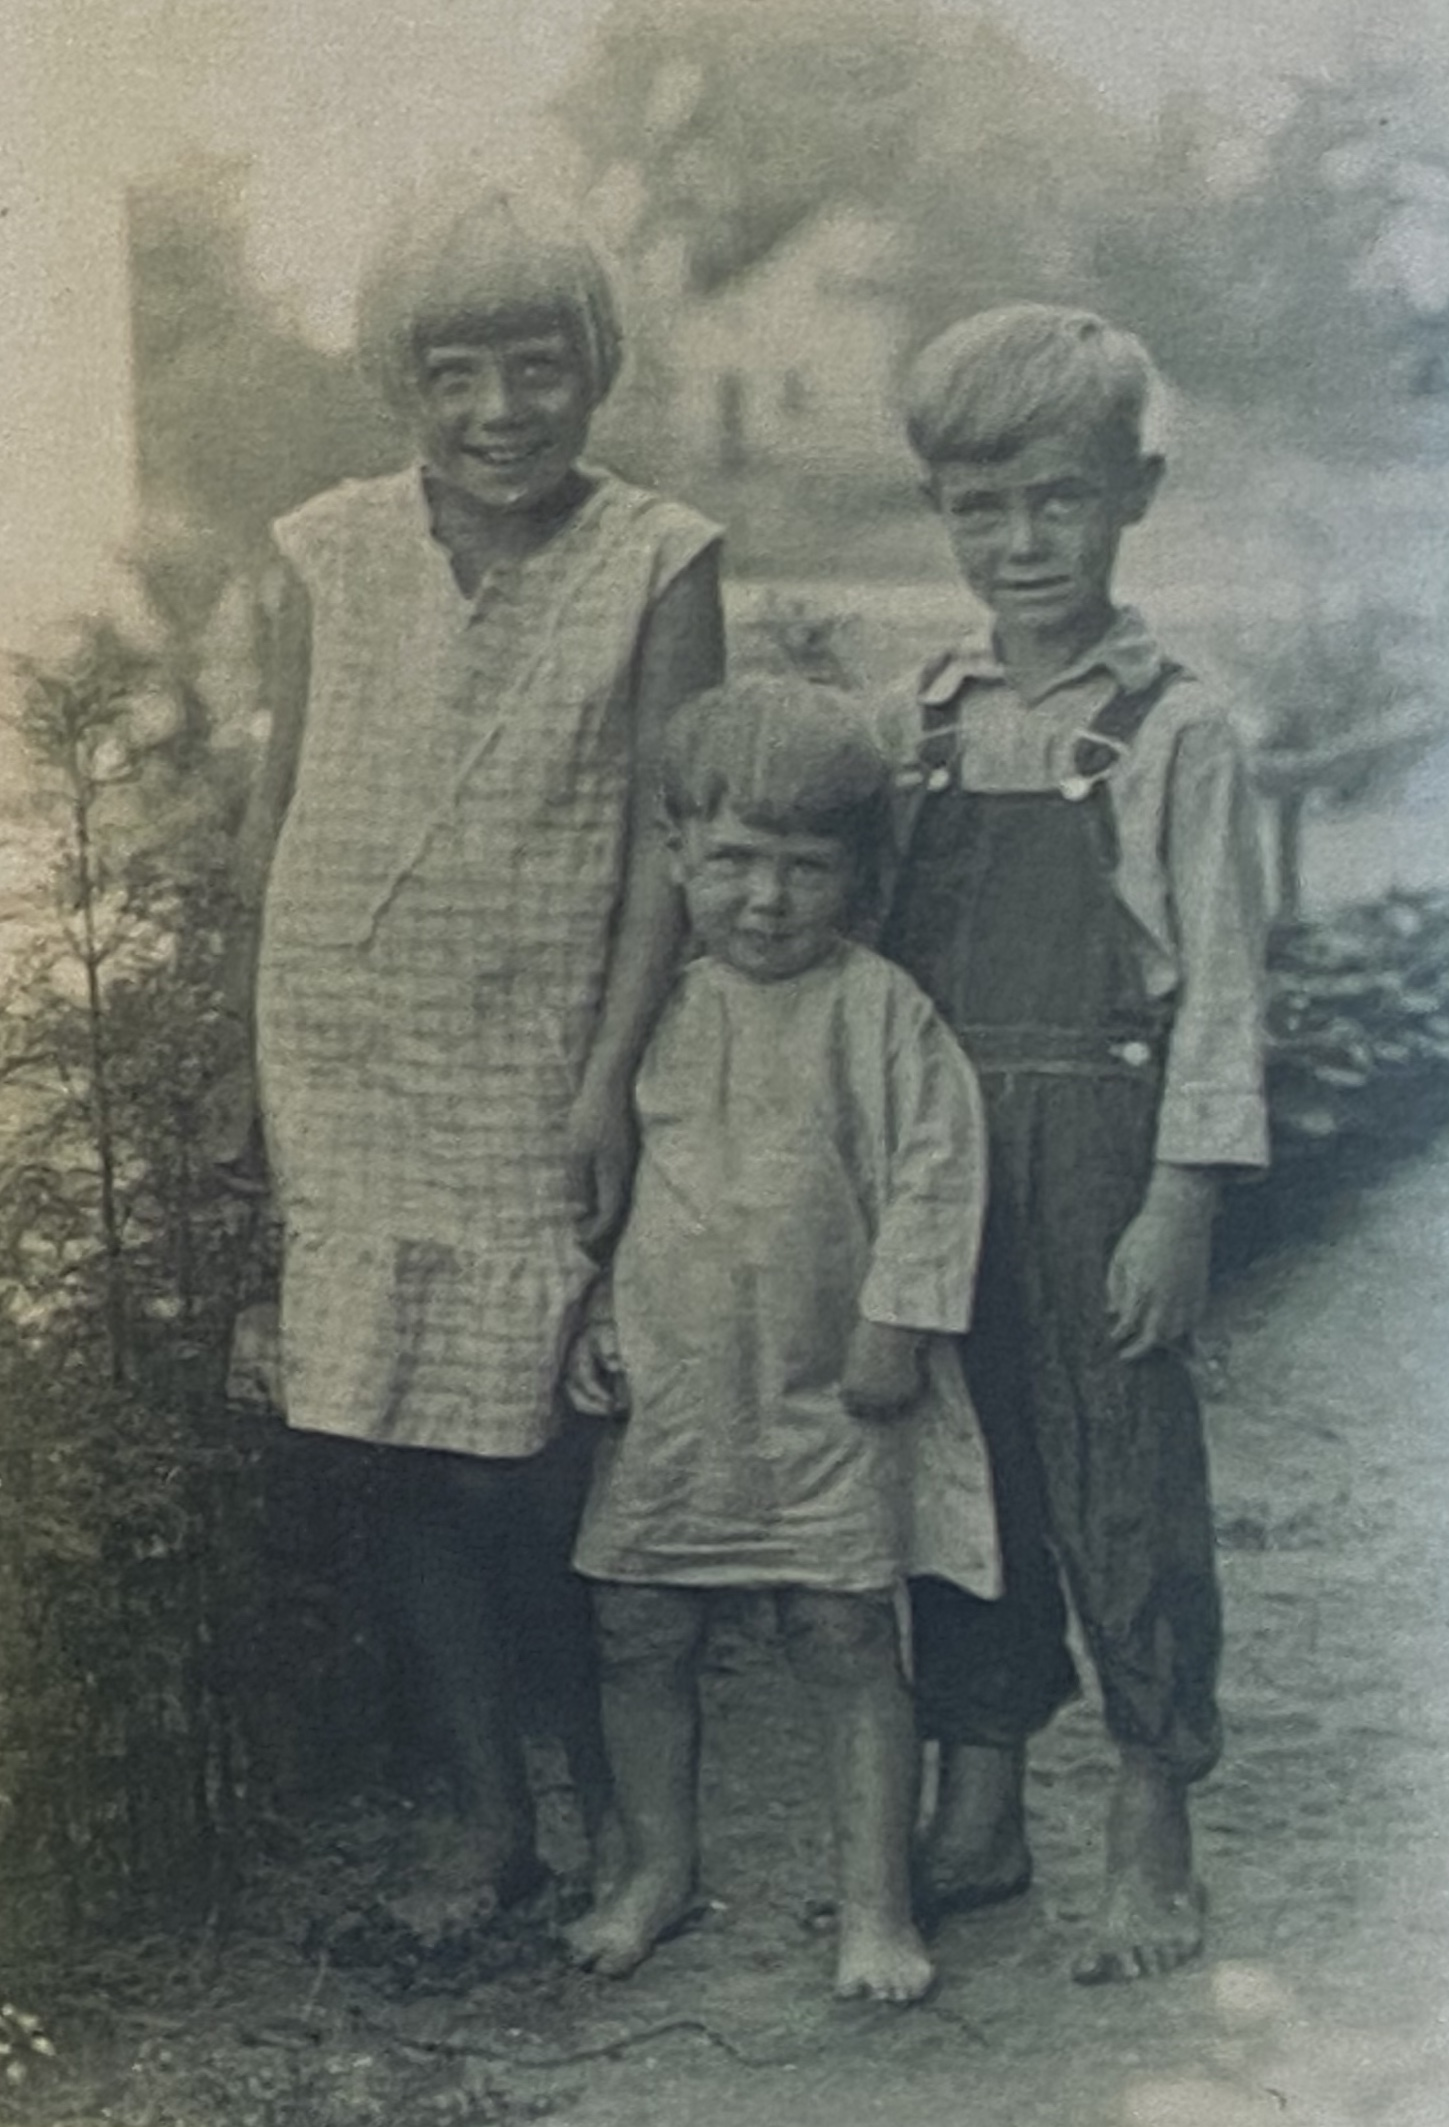
\includegraphics[width=0.7\linewidth,height=\textheight,keepaspectratio]{images/Akou02.JPG}

}

\caption{Lila with her younger brothers, Earl and Looy, c.~1931}

\end{figure}%%
\begin{figure}[H]

{\centering 
\includegraphics[width=0.8\linewidth,height=\textheight,keepaspectratio]{images/Akou03.jpg}

}

\caption[Members of the Slaback Family 1922--1958]{I developed this
chart using \href{https://www.ancestry.com/}{Ancestry.com} and census
records. Only people who were alive during Lila's lifetime are listed;
younger children and later generations are not. The fathers of Lila's
last four children are speculative but are included as a reference for
readers.}

\end{figure}%

\section{Notes}\label{notes-1}

I have no idea who originally took these family photographs. Some of
them came from my mother's sister, June. Others I inherited when my
mother passed away.

The first section of this book, ``The Slaback Family,'' is told from
Lila's perspective using words and observations that a child (and later,
a teenager) would make. As one of the younger children in a large
family, she would not have received much attention from her parents. I
imagine that her oldest sister, Izro, was more like a mother to her.

\bookmarksetup{startatroot}

\chapter{Chapter One}\label{chapter-one}

Lila was five years old when her family moved to La Crosse. She told her
doll, Elizabeth, ``Don't be scared. I won't let anything happen to
you.'' There was barely enough room in the wagon for everyone to sit.
Izro made her sit in her lap. She didn't want to---she wasn't a baby!
Earl, who was only three years old and the real baby of the family, sat
in their mother's lap. Izro whispered into her ear, ``Are you excited
about getting on the train?'' She nodded her head. Her parents had been
planning this trip for a long time. They were moving to a new house in
the big city. Lila could tell that everyone was excited.

In truth, Lila was also sad. She was thinking about her cat, Annabelle,
and how she would never see her again. One of the cats that lived in
their barn had a litter of kittens the year before. Annabelle was the
only one that survived. She was a tiny ball of gray fluff when Lila
picked her up and carried her into the house. Her mother ordered her to
take it back outside, but Lila was in love. The kitten was so soft and
had beautiful green eyes. She kept sneaking the kitten back into the
house until finally, her mother gave up and said the cat could stay.
Lila fed Annabelle scraps from her plate until she was old enough to
hunt for mice. She didn't stay in the house very long. Lila looked for
her whenever she went outside. There were plenty of other animals around
the farm, but Annabelle was the only one that was truly hers. That
morning with all the commotion, Lila had not been able to find her. She
looked in the barn, behind the house, under the chicken coop, down by
the creek---everywhere she could think of---but Annabelle was not there.
(She didn't know it, but Annabelle was hiding with her first litter of
newborn kittens.) She was too old to cry about it. Her brothers would
have teased her for caring so much about a stupid cat. Izro was busy
helping with the cleaning and her mother never wanted the cat in the
first place. There was nothing that could be done, so Lila tried not to
think about it.

Lila had never been on a train before. On quiet nights she could hear
their whistles off in the distance, but she had never seen one up close.
Her father purchased tickets from the man who ran the grain elevator and
they sat on their trunks to wait, which were packed with everything they
owned. The first train, which took them from Soldiers Grove to Prairie
du Chien, had only one car for passengers. The rest of the train was for
hauling freight. Aside from the conductor and the brakemen, the Slabacks
were the only people riding the train that day. Lila's mother insisted
that she sit next to her on the hard wooden bench. Earl was getting
fussy, but he stopped as soon as the train started moving. Veda, who was
two years older than Lila, sat next to her. She was smiling, but Lila
noticed that she was gripping the bench like it was the only thing
saving her from certain death. It seemed like everyone was holding their
breath as their seats rumbled and the train picked up speed, taking them
away from Crawford County.

Hazel and John had both grown up in Crawford County. John had inherited
the family farm from his parents, Levi and Amy Slaback. Although he was
the youngest of nine children (since his younger brother, Warren, had
been killed as a young child when he was kicked in the head by a cow),
most of them were girls who had gone to live with their husbands as soon
as they got married. Elmer, John's older brother, was good at math in
school and decided that he didn't want to be a farmer. He had started
his own business as a builder and was living with his wife and five
children in a different town. Frank, his much older brother, had waited
so long to get married that everyone thought he would be a bachelor
forever. His wife, Hattie, was a widow with two children when they met.
They had moved to the big city of La Crosse, where Frank found a good
job as a cutter at the rubber mill. Lila didn't know it at the time, but
Hattie was also working outside of the home at a restaurant for tourists
known as The Pearl.

Lila wished that she had been allowed to sit by the window, but at least
she could see the tops of the trees as they flew past. It took less than
an hour to reach Prairie du Chien, which had a special building just for
train passengers. While her father went over to a man standing behind a
window to purchase more tickets, the rest of the family sat down by the
big clock in the middle of the room and started eating their lunch,
which they had carried with them in a basket. Soon it was time to get on
the train again. This one was just for passengers. The cars were shiny,
and the benches had cushions with soft fabric. It was so comfortable and
very fast---much faster than the first train. Lila's mother relaxed a
bit and allowed her to stand by the window so Lila could see what was
happening. Not long after they left the station the trees cleared, and
she could see an enormous stretch of water. It was dark blue and there
was a long, flat boat being pulled by a smaller boat. Her brother,
Theron, told her it was the Mississippi River. Lila didn't know there
was that much water in the world. Already, the landscape was very
different from the farm.

Although she didn't mean to, Lila fell asleep on the train. One minute
she was watching the river and the next minute Izro was telling her,
``Wake up, Lila. We need to get off the train and you're too big to
carry.'' They had arrived at another train station, but this time they
were not going inside. Uncle Frank was waiting for them with a truck.
``Welcome to La Crosse!'' he said and gave Lila's mother and father a
warm hug. When John was thinking about getting out of farming, he and
Theron traveled to La Crosse and stayed with Frank and Hattie for a few
days. During the last long winter on the farm, they had shared their
stories about the city so many times---about the tall buildings, the
cars, the places to shop, and the crowds of people dressed in fancy
clothes---that to Lila, the city already seemed like a familiar friend.

As they stood in the train station, Lila counted her brothers and
sisters and parents and Uncle Frank. Ten people. She wasn't in school
yet, but she was proud that she could count. Izro had taught her how.
Her father left to find the trunks and her uncle said, ``Who wants to go
first?'' Her mother decided that she would go, taking Izro and the
younger children. Their new house was on the northern edge of the city.
John had built it with help from Elmer, who knew the best places to buy
lumber and fixtures. Hazel wanted to open the windows and let in some
fresh air before they moved everything inside.

There was just enough room in the front of the truck for Uncle Frank,
Hazel, Izro, Veda, Lila, and Earl. Lila sat in Izro's lap again and for
once she was glad. A truck was much faster than a wagon. What if they
crashed? What if Uncle Frank drove into the river? They closed the doors
and started driving down the street. Lila was relieved that he wasn't
driving too fast. By the time they reached their new house, she thought
maybe driving wasn't so bad.

\section{Notes}\label{notes-2}

This chapter establishes some important facts about the Slaback family.
John and Hazel grew up in Crawford County, Wisconsin on farms that were
less than one mile apart. When they were first married, they moved to La
Farge, Wisconsin (near John's brother, Elmer), but they moved back to
Crawford County in the early 1920s to take over the farm owned by John's
parents, Levi and Amy Slaback. John was the only living son who
attempted to make a living as a farmer.

There had been a rapid expansion of the railroad system in rural
Wisconsin, which led farmers to make a choice: buy a tractor, acquire
more land, and start farming cash crops (a choice made by my paternal
grandfather's parents), or sell the land and move to the city. John and
Hazel Slaback made the latter choice. When they left the farm, they
already had seven children. John's oldest brother, Frank, was the first
member of the Slaback family to move to the big city of La Crosse. At
the time, it was one of the largest cities in Wisconsin outside of the
Milwaukee area.

Many farms in Wisconsin have ``barn cats'' that are largely feral and
help to catch mice. I have no idea if Lila really owned a cat, but this
chapter establishes Lila's caring nature and how barn cats are typically
treated (tolerated, but not loved). It would have been heartbreaking to
leave a cherished pet behind, especially knowing that nobody else cared.

I have no idea how John's brother Warren died, but he was young. Getting
kicked in the head by a cow is a very Wisconsin way to die. Cows are
usually gentle, but they're also very strong and can be deadly when
provoked.

The train was a plausible way for a large family to travel from Crawford
County to La Crosse. It is highly unlikely that John and Hazel Slaback
would have owned a truck before moving to the city. In the 1920s,
farmers commonly used horse-drawn wagons for transportation.

For more information, see Wisconsin Legislative Reference
Library\footnote{\citeproc{ref-wisc1952a}{{``The Development of
  Wisconsin Population, 1840--1950''} (Wisconsin Legislative Reference
  Bureau Digital Collections, 1952),
  \url{https://cdm16831.contentdm.oclc.org/digital/collection/p16831coll2/id/482/}}.},
Richard Nelson Current\footnote{\citeproc{ref-current1977a}{\emph{Wisconsin:
  A History} (1977; repr., {Urbana and Chicago}: University of Illinois
  Press, 2001)}.}, Elizabeth Sanders\footnote{\citeproc{ref-sanders1999a}{\emph{Roots
  of Reform: Farmers, Workers, and the American State, 1877--1917}
  (University of Chicago Press, 1999)}.}, and William John White
III\footnote{\citeproc{ref-white2000a}{{``An Unsung Hero: The Farm
  Tractor's Contribution to Twentieth-Century United States Economic
  Growth''} (PhD Dissertation, The Ohio State University, 2000)}.}.

\bookmarksetup{startatroot}

\chapter{Chapter Two}\label{chapter-two}

Early the next morning, Lila woke up and realized that it had really
happened---they were in the new house. She was in her new bedroom,
sharing a bed with her two older sisters, Izro and Veda. It was cozy and
warm under the quilt. Last night they had taken their clothes out of the
trunks, hanging them on nails around the bedroom. Lila's doll,
Elizabeth, was waiting patiently on a bench next to the bed, along with
Veda's doll, Francine. It was still quite cold at night, so Izro had
closed the window before they went to bed. The house smelled like fresh
wood, but there was another good smell; her mother was cooking eggs and
bacon. Her older brothers were laughing. Lila slipped out of bed and
walked to the bathroom next door. She could hardly believe that they
lived in a place where it was no longer necessary to use the
outhouse---they didn't even have an outhouse! In the back there was just
a garden, waiting for them to plant new seeds. The night before, Izro
told her that she should wash her hands every time she went to the
bathroom. There was a bar of soap sitting in a bowl next to the sink and
a piece of cloth hanging on the wall. It was a thrill to turn the taps
and watch the water rushing into the basin. Lila had played in the creek
behind their old house, diverting the water with sticks and mud and
watching it rush back out when the ``dam'' broke. It was fun, but most
of the year it was too cold to play in the creek. The sink had one tap
for cold water and one for hot water. How did the water get hot?

When she went back to the bedroom, Izro and Veda were starting to wake
up. Izro said, ``Let's get both of you dressed.'' Lila and Veda
dutifully took off their nightclothes and put on their dresses. Izro
combed Lila's hair and tied it back with a strip of cloth. Lila and Veda
were wearing nearly identical dresses; their mother had made them from
the same pattern, using blue fabric for Lila's dress and green fabric
for Veda's. They fit loosely and had strings at the top to adjust the
neckline. At the bottom, they had neat lines made by hemming extra
lengths of fabric. The hems could be removed as necessary to make the
dress longer. Izro had recently removed two of the lines from Veda's
dress because she was having a growth spurt. It wouldn't be ladylike to
wear a dress that was too short. Since it was not very warm yet, they
would have to put on their stockings, shoes, and sweaters before going
outside. Lila hated all the layers because the wool was so itchy.
Inside, their dresses were enough.

Veda had beautiful hair that was nearly golden and liked to have it
braided, so Izro did that, and then the two younger girls skipped off
for breakfast. Izro stayed behind to change her clothes and comb her own
hair. She would join them soon. Lila sometimes let Izro braid her hair,
but it was a challenge to sit still. She preferred to leave it loose,
even though Izro teased her that she looked like a ``wild animal'' with
her hair down.

Later that morning, while Izro was helping her mother clean up from
breakfast and start preparations for lunch, Lila and Veda went outside
to explore the neighborhood. Earl was too young to go with them and
Cecil was too old---he was eleven and wanted to see what his older
brothers were doing; he didn't want to spend the day with two girls.
That first day, they were only brave enough to walk around the block. By
the end of the week, they were crossing the street and exploring the
neighboring blocks. There were so many houses! Some were tiny and some
were large; they had many different colors and shapes. A few had fences,
but mostly Lila and Veda could see into their yards. Many of the houses
had gardens and lines for hanging wet laundry; a few had an extra
building for a car. One of their neighbors even had a little house just
for his dog. It was a big black dog with curly hair, and he was not very
friendly. When he started barking, they would walk as quickly as they
could until that house was behind them. One day the dog's owner came out
and yelled, ``Stop bothering the dog!'' Lila thought it wasn't
fair---she wasn't doing anything to make the dog act that way---but good
girls didn't talk back. She and Veda put their heads down and walked a
little faster. They said nothing to their parents. Veda was always
ashamed to be scolded and did her best to avoid it.

As the weeks passed, they started discovering other children. Edith and
Margot's parents were very strict and spoke German. Lila and Veda could
visit, but Edith and Margot were never allowed to go beyond the family's
yard without their parents unless they were walking to school. Their
father was a beer maker who lost his job because of Prohibition. Ruth,
Anna, and Magnus had recently come from Norway. Their mother didn't
speak any English, but she made delicious cookies. Margaret didn't have
any brothers or sisters. What a surprise! She lived in a tiny blue house
and had several pets: a cat, a dog, and a pair of yellow birds that
lived in a beautiful cage. Lila was jealous. She missed her cat,
Annabelle, and wondered how she was doing. Margaret's mother was a sweet
woman who always invited the girls in for sandwiches. Some days, Lila
and Veda forgot to go home for lunch. The first few times their mother
scolded them, but eventually she decided that it was fine as long as
they were back in time for dinner.

Izro had warned them to stay away from the river. It wasn't like the
creek behind their house on the farm. The section closest to their
neighborhood was the Black River and not the Mississippi (it joined the
Mississippi at French Island), but the current was still very strong,
and it was not safe to play around. One hot day that summer, Lila and
Veda decided to go down to the water and dip their toes in. What could
it hurt? The cool water felt delicious on their feet. Veda stayed at the
edge, but Lila started splashing and wading in a bit deeper. Veda said,
``Lila, what are you doing? We're not even supposed to be here!'' but it
was like her voice was muffled. It was so pleasant to feel the water
swirling around her legs and wetting the hem of her dress. All of a
sudden, she was completely under the surface. The water instantly filled
her mouth and nose, but her eyes were still open. Not that it mattered,
because the river was so murky that Lila could barely see anything.
Before she could panic, Lila felt a tug on the back of her dress. A man
living on a houseboat had noticed the girls playing by the river and
sprinted over as soon as Lila disappeared. ``What are you doing here?''
he yelled. ``Go home and don't come back! It's not safe!'' The girls
both started running.

As soon as they were out of the man's sight, Veda burst into tears. She
kneeled on the ground and covered her face with her hands. The water
from Lila's dress and hair was pooling at her feet, turning the dust
into mud. What were they going to tell their parents? Once Veda had
calmed down, she decided they should stand there until Lila was dry.
``If the neighbors see you like that, someone will tell Mom and Dad for
sure.''

\begin{figure}[H]

{\centering \pandocbounded{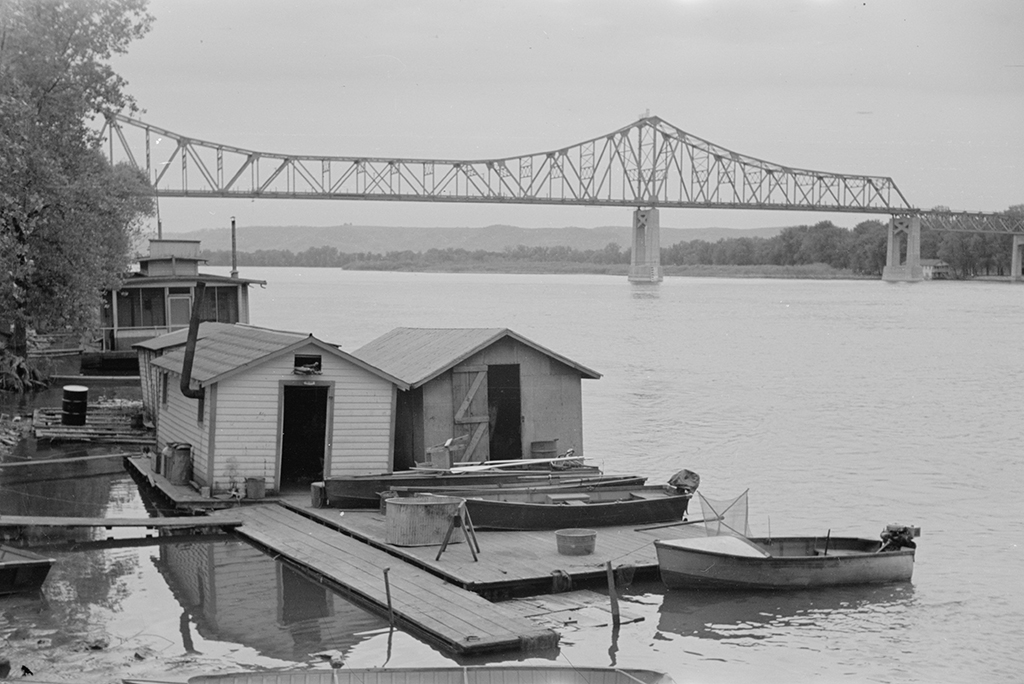
\includegraphics[keepaspectratio]{images/Akou04-enlarged.jpg}}

}

\caption[Houseboats along the river in La Crosse]{Houseboats along the
river in La Crosse. Library of Congress Prints and Photographs Division,
\#LC-USF33-003063-M4. Photograph by Arthur Rothstein (1915--1985) in
1939.}

\end{figure}%

\section{Notes}\label{notes-3}

From Zillow, I learned that the house Lila grew up in (which is still
standing) was built in 1928. That's where the family was living in 1930;
I assume my great-grandfather built it. His brother, Elmer, was a
builder and could have easily given him advice. I used Zillow to look at
nearby houses to imagine a floor plan. At the time, the neighborhood was
on the very northern edge of the city. I used historic plat maps to get
a sense of how the city was growing in the early 1900s. The blocks were
only partially filled with houses; many were inhabited by migrants from
rural areas and other countries (mostly Germany, Ireland, and
Scandinavia).

A lot of this chapter draws from things I know as a fashion historian or
experienced as a small child growing up in Wisconsin. In the early
1900s, working-class families owned very little clothing---often just
one or two outfits to wear on a daily basis and one nice outfit for
church. Most houses did not have closets. Adjustability was essential
for children's clothing. I'm sure my mother had dresses with extra tucks
as a child. When I was growing up, she pointed them out to me repeatedly
with a nostalgic tone of voice. Layering is essential in Wisconsin,
where the winter (snow on the ground) essentially lasts from November to
April. As a child, I hated itchy wool sweaters, scarves, and mittens.

Until I was in fourth grade, I always had long hair. My mother spent a
lot of time making it look just right. If I resisted, she told me that I
looked ``wild'' or ``like a banshee.''

When I was two years old, I nearly drowned in the Eau Claire River. It
was springtime and my father was an avid fisherman. The current was very
fast. The riverbank where I was standing collapsed, and I fell in. I
don't remember falling in, but I remember my father pulling me out and
how cold it was! He wrapped me in a blanket and turned up the heat in
the car. I remember the look on my mother's face when my father
explained why I was drenched. To this day, I have a healthy fear of
fast-moving water.

When I was in elementary school, my family went camping sometimes. A lot
of campgrounds and cabins in northern Wisconsin still had outhouses.
Like Veda and Lila, my sister and I were close in age and spent a lot of
time together exploring the neighborhood. The story of the black dog who
wouldn't stop barking is based on one of my childhood experiences.

For more information, see Susan Porter Benson\footnote{\citeproc{ref-benson2007a}{\emph{Household
  Accounts: Working-Class Family Economies in the Interwar United
  States} (Ithaca: Cornell University Press, 2007)}.}, Andrew J.
Cherlin\footnote{\citeproc{ref-cherlin2014a}{\emph{Labor's Love Lost:
  The Rise and Fall of the Working-Class Family in America} (New York:
  Russell Sage Foundation, 2014)}.}, and Jane Farrell-Beck and Jean
Parsons\footnote{\citeproc{ref-farrell-beck2007a}{\emph{{20\(^{th}\)-Century}
  Dress in the United States} (New York: Fairchild, 2007)}.}.

\bookmarksetup{startatroot}

\chapter{Chapter Three}\label{chapter-three}

Shortly after they arrived in La Crosse, Uncle Frank and Aunt Hattie
took the family to Grandad Bluff for a picnic. There was a park at the
top with a magnificent view of the city. Lila had met Uncle Frank the
day he picked them up from the train station, but it was her first time
meeting Aunt Hattie and her cousins, Kenneth and Lloyd. Hattie was
taller than her mother and older too---more like a grandmother than an
aunt. She was wearing a light blue dress with short sleeves, a long
string of beads, and a matching hat with a darker ribbon. Lila didn't
mind when Aunt Hattie leaned down to give her a little hug; her dress
was soft, and she smelled like flowers. (That night, her mother made a
comment about the short length of Hattie's dress and how scandalous it
was for a woman her age to dress that way.)

Her cousin Lloyd was seventeen---almost the same age as her brother,
Lyle, except that he was the youngest in the family. He had wild black
hair and dark eyes with a look of mischief. Lila heard her uncle say
that Lloyd had left school and was training to be a cabinet maker; maybe
he could work for John. Lila felt a mixture of excitement and
nervousness around Lloyd. Her own brothers ignored her most of the time,
but Lloyd did not. They played a thrilling game where Lloyd held her by
the feet and spun her around in a tight circle with her arms and hair
flying out. Veda didn't want to give it a try; she said just watching
made her feel dizzy. Lila and Earl took turns until Aunt Hattie said
sternly, ``That's enough now.''

Lila, Izro, and Aunt Hattie went into the kitchen to finish preparing
the lunch. The night before, Izro had baked several loaves of bread and
pound cake. They put some in a basket along with a container of butter,
some jars of pickles (which Hazel had made from the tiny beets and
cucumbers that were just starting to appear in their garden), a big
block of cheese, a sack of fresh peas, and two jars of strawberry jam.
They also added a knife to cut the bread and cheese, a cutting board,
cups for water, and some plates and silverware. Lila's mother commented
that the younger children would not need plates; they could hold their
sandwiches and wander off to play. Lila thought that was a good plan;
maybe she wouldn't have to eat the peas. She didn't really like them,
but children had to eat whatever food they were given. It was a rule.

When the picnic basket was ready, the group filed out the front door.
They would walk together to the nearest streetcar line and then ride the
rest of the way. Lila's father carried Earl on his shoulders. Although
she knew it was wrong, Lila felt a bit jealous. She consoled herself by
thinking, ``At least I'm old enough to walk on my own. I don't need to
be carried.'' Before she knew it, they had reached the first stop on the
streetcar. It was five cents to ride. Uncle Frank paid for the tickets.
The first streetcar took them past Frank and Hattie's house (Lloyd
pointed it out to his cousins). When they reached downtown, they
switched to another streetcar that would take them down Main Street and
up the hill, close to the top of the bluff. Built on a plain next to the
Mississippi River, most of the city was flat. Although the bluffs on the
other side of the river went all the way to the shore (which made it
impossible to farm and difficult to build houses), Grandad Bluff was two
miles east of the river. In the summer, it was popular for families to
go hiking and take picnics. Aunt Hattie had been there many times with
her friends. When the line ended, it was just a short walk into the
park.

At the edge of the park, there was a wooden deck where you could go to
get the best view. Lila went up to the railing, but Veda shook her head
and refused, saying that it was ``too scary.'' They were high above the
city. Lila wondered if she could spot their house. She found the bridge
that went over the river and was looking around trying to find their
neighborhood when suddenly she heard, ``Lloyd Spencer Slaback, you get
away from there this instant!'' Aunt Hattie was furious. Instead of
staying on the deck, Lloyd was going around the railing to the very edge
of the cliff. Lloyd laughed and said, ``I was just trying to have fun.''
Lila felt sick to her stomach. It made her nervous for Lloyd: nervous
that he could fall, but also worried about what Uncle Frank would do to
him once they got home. If her brothers behaved that way, her father
would have hit them with a belt. Aunt Hattie went back to talking with
Lila's parents like nothing was wrong, but Lila wasn't able to eat much
when it was time for lunch.

\section{Notes}\label{notes-4}

Before I started this project, I had never heard of Uncle Frank and Aunt
Hattie. From census records, I learned that Hattie was originally from
Michigan. Her father served in the Civil War; after the war, he moved
the family from Michigan to Wisconsin. Hattie married when she was only
fifteen years old and had two children with her first husband, Frank
Udell, before he died in 1899. In 1902, she married Frank Slaback, who
was 35 years old. It was his first marriage; I imagine the Slaback
family had given up hope that he would ever get married.

For three years, Hattie lived as a single mother. In the 1900 census she
was listed as ``head of household.'' She and Frank Slaback had three
more children and moved to La Crosse shortly before World War I when
Hattie was approximately 40 years old. She was working outside of the
home and had her own listing in the phone directory. For the time, this
was an astonishing amount of independence. Frank was also working at the
La Crosse Rubber Mills; having two incomes would have lifted the family
into the middle class, but I imagine that Aunt Hattie was regarded with
intense suspicion by more conservative members of the Slaback family.

Until the 1940s, Hattie Slaback was the only member of the family listed
in the society pages of the newspaper. Fortunately for me, Slaback is an
uncommon name, so it was not too difficult to sort through historic
newspapers and find mentions of the family.

This chapter helps readers understand the visual landscape of La Crosse.
As a child, I visited all the places in this book, including Grandad
Bluff. My cousin, Paul, was a teenager at the time; he did exactly what
Aunt Hattie scolded Lloyd for doing. The foods that they took on the
picnic are the kinds of things that would have been available in late
spring for a working-class family with a backyard garden.

My parents were both middle children in large families, so I grew up
with many cousins. It was a thrill when the older cousins would play
with me or let me tag along on their adventures. The activity of
spinning in a circle (or being spun)---often to the point of
dizziness---was something I did many times as a child. I spent a lot of
time outdoors, regardless of the weather.

For more information, see Eric J. Morser\footnote{\citeproc{ref-morser2003a}{{``Manufacturing
  Pioneers: Commerce, Government, and Manhood in La Crosse, Wisconsin,
  1840-1900''} (PhD Dissertation, University of Wisconsin, 2003)}.},
William Barillas\footnote{\citeproc{ref-Barillas2006a}{\emph{The
  Midwestern Pastoral: Place and Landscape in the Literature of the
  American Heartland} (Athens: Ohio University Press, 2006)}.}, John
Nolen\footnote{\citeproc{ref-nolen1911a}{\emph{The Making of a Park
  System in La Crosse} (La Crosse: The Inland Printing Company, 1911)}.},
and Guide to the Mississippi Valley Public Service Company
Records.\footnote{\citeproc{ref-mississippi1914a}{{``Guide to the
  Mississippi Valley Public Service Company Records, MSS 028''} (La
  Crosse Public Library Archives, 1914-\/-1942),
  \url{https://archives.lacrosselibrary.org/collections/businesses/mss028/}}.}

\bookmarksetup{startatroot}

\chapter{Chapter Four}\label{chapter-four}

That fall, there were two big changes. At the beginning of September, a
new baby came to live in the Slaback house. Lila had noticed that her
mother was getting bigger, but she didn't really understand why. She was
only two years old when Earl was born. (She didn't know it, but her
older siblings had learned about pregnancy by watching the cows on the
farm. Lila and Earl were the only members of the family surprised to get
a new brother.) Looy hardly slept. For the first few months, it seemed
like he would never stop crying. He was healthy, but his little face
would get dark red and he would cry for hours. The only way to soothe
him was to bounce him or take him outside for a walk in the fresh air.
All he did was cry and throw up and make stinky diapers. Looy's arrival
made Hazel even more impatient and angry than usual.

The second big change impacted Lila more directly. A few weeks after
Looy's birth, John took Lila, Veda, and Cecil to register for school.
Lila had not been old enough to attend when they lived in Crawford
County, so it was a new experience. She had a lunch pail that Izro had
filled with an apple and some sandwiches wrapped in a piece of cloth.
The school was so big that there were many different classrooms. Lila
was shocked when her brother and sister were led away to other parts of
the building. She would be in first grade and was assigned to Miss
Miller as a teacher. One of the women from the office took her hand and
said, ``Come with me, young lady.'' They walked down a long hallway past
several other doors and the woman said, ``This is the one!'' There were
many other children already inside the classroom. Miss Miller was
standing at the front of the room and asked her to sit at one of the
desks. Lila chose a seat next to a girl with freckles and curly red
hair. She smiled and the other girl smiled back. The desk was smooth,
with curlicues of metal on the sides. Most of the room was filled with
desks lined up in neat rows. Lila would spend many hours running her
fingers around the curlicues to pass the time. The boys liked to sit in
the back so they could make jokes and cause trouble, but Lila was
determined to be a good girl and sit quietly in her seat.

Miss Miller had all the letters of the alphabet written on the
blackboard and asked the students to copy her writing on their slates.
Lila was astonished to realize that her desk had a slate and two pieces
of chalk inside\ldots every student had one. Even more astonishing was
the next week when Miss Miller handed out books: they were blue, and she
gave a copy to every student. Lila had never held a book. She knew about
reading---her parents and older brothers sometimes read aloud from the
newspaper while the rest of them listened. Miss Miller said, ``Please
keep these inside\ldots{}'' but Lila barely heard her instructions. The
book was filled with colorful pictures of animals and children. The
first story was about two children and a mother cat. She thought they
must be on their way to church; the girl had a big white bow in her
hair, a frilly white dress, and blue socks. Lila didn't have such fancy
clothing, but she was satisfied with her appearance. She was more
interested in the pictures of the animals.

During lunch, Lila was relieved to see her sister and brother and many
of the children from her neighborhood. Some of the boys were playing a
rough and silly game of Red Rover. She quietly ate her sandwiches, not
talking or being asked to talk---nothing out of the ordinary. At home,
her parents and older brothers did most of the talking. They talked
about the new truck (which was for work, not for the family to ride in),
what lumber mills had the best prices, where they could sell the extra
vegetables from the garden, who was building a new house two blocks
away, and when they might have guests over to play cards. Even if Lila
had a chance to speak (which was rare), the adults were not interested
in that scary dog on the next block, what kind of cookie was Lila's
favorite (chocolate chip), or what happened at school that day. The
world was a place for adults and Lila would just have to wait her turn.

\section{Notes}\label{notes-5}

Loyal (Looy) was the first member of the Slaback family to be born in La
Crosse. My younger child had colic due to a severe dairy intolerance, so
that experience informed my description of Looy's behavior and how it
impacted the rest of the family. I was losing my mind from lack of
sleep. I don't know what I would have done if I had seven other
children!

Roosevelt Elementary, named after Theodore Roosevelt, was the
neighborhood school for young children on the north side of La Crosse.
In Crawford County, the local school stopped at eighth grade; there was
no high school in the 1920s. The 1940 census notes that John Slaback
dropped out of school after fifth grade; Hazel dropped out after seventh
grade. The two oldest children, Theron and Izro, finished school in
eighth grade; they were too old to enroll in high school when the family
moved to La Crosse.

I used \href{https://archive.org/}{archive.org} to look at historical
examples of elementary school textbooks from the early 1900s. It is
impossible to know exactly what textbook(s) Lila learned to read from,
but two possibilities are \emph{McGuffey's First Eclectic Reader} and
the \emph{Elson-Gray Basic Reader} (better known as the precursor to the
``Dick and Jane'' books).

As a small child, a family member gave my parents a set of old-fashioned
school desks. The first part was just a seat, and the last part was just
a desk---they were secured to metal tracks and were clearly designed to
be placed in longer columns. They were painted red with black
wrought-iron curlicues on the sides. It was easy for me to imagine what
a 1930s classroom might have looked and felt like. Red Rover was a game
I played as a child. My children played it too.

At the dinner table in my household, I was expected to be ``seen and not
heard.'' Conversation revolved around adult topics. Card-playing was a
common entertainment for the adults when I was a small child. My parents
taught me to play games like cribbage, rummy, spades, King's Corners,
and solitaire. We had a television, but there were only a handful of
channels.

I spent a lot of time reading as a child; my dad often took me to the
public library to feed my appetite for new books. My older child is
dyslexic; I've often thought about how boring and frustrating my
childhood would have been if I did not have books for entertainment. I
don't know if Lila was dyslexic, but learning disabilities were barely
recognized back then.

For more information, see La Crosse Public Library Archives \& Local
History Department\footnote{\citeproc{ref-lacrosselibrary2022a}{{``The
  Way It Was: Roosevelt School, Circa 1931,''} May 22, 2022,
  \url{https://lacrossetribune.com/the-way-it-was-roosevelt-school-circa-1931/article_66e6c3d6-d9fa-11ec-b99f-83bfbe095d45.html}}.},
James Hinshelwood\footnote{\citeproc{ref-hinshelwood1917a}{\emph{Congenital
  Word-Blindness} (London: H. K. Lewis \& Co. Ltd., 1917)}.}, Kate
Kelly\footnote{\citeproc{ref-kelly2017a}{{``Dick and Jane: Story of
  These Early Readers,''} June 2, 2017,
  \url{https://americacomesalive.com/dick-and-jane-story-of-these-early-readers/}}.},
and Nikki Katz\footnote{\citeproc{ref-katz2012a}{\emph{The Book of Card
  Games: The Complete Rules to the Classics, Family Favorites, and
  Forgotten Games} (New York: Simon; Schuster, 2012)}.}.

\bookmarksetup{startatroot}

\chapter{Chapter Five}\label{chapter-five}

One night that fall while the family was eating dinner, Theron said that
he needed to make an announcement: he was planning to get married.
Lila's mother stood up, handed the baby to Izro, and went over to Theron
to give him a big hug. Although she had tears in her eyes, she was
clearly not sad. She said, ``Oh Theron, I'm so happy for you!''

Lila turned to Veda and said, ``What does that mean?''

Veda said, ``Theron wants to have a wife so they can become a mommy and
daddy.''

It wasn't long before she heard the word ``marriage'' at school. Some of
the girls were playing a clapping game: ``First comes love, then comes
marriage, then comes the baby in the baby carriage!'' Is that what her
parents had done? Lila had learned where babies came from thanks to her
new little brother but thought she knew nothing about love and marriage.

A few weeks later, a stranger named Myron arrived at their house for
dinner. It wasn't that unusual to have a guest over. Maybe he was one of
her brother's friends. Lila's father shook his hand, and the men went
out to the backyard to look at the garage and the truck while Izro and
her mother finished cooking. Izro handed a stack of plates to Veda and
the silverware to Lila and told them to go set the table. She wasn't
exactly rude about it, but she seemed nervous---not her usual self. Lila
noticed that her cheeks were pink.

At dinner, they talked about Myron's family. His parents had lived in La
Crosse and his mother was best friends with Aunt Hattie before they
moved to Onalaska. His parents were from Norway and changed their names
from Lars and Anna to Louis and Antoinette. (Lila thought that was
fascinating; she had no idea that it was possible to change your name.)
There were seven children in Myron's family, three girls and four boys.
He was the youngest son, the sixth out of seven kids, the same as Lila.
It was nice to hear about something besides lumber prices and
vegetables. Then Myron said, ``Mr.~Slaback, what I came to ask you
is\ldots would you allow me to marry your daughter, Izro?'' Lila's
mother had been so happy when Theron said he was getting married, but
that night she was very quiet. Lila was confused about the difference in
her reaction. Was she angry at Myron for some reason? Did she not want
Izro to get married? Her father said ``Yes,'' and her older brothers
gathered around to laugh, slap Myron on the back, and say, ``Welcome to
the family!'' Lila looked across the table at Izro and thought she must
be running a fever because her cheeks had turned from pink to red.

The family decided to have a double wedding in January, and it was very
cold---the kind of cold where the snow is crunchy and screams when you
step on it. Lila was still on vacation from school, and she was wearing
a new dress that her mother had made on the sewing machine. It was the
same shape as the other two dresses she wore to school, but this one was
thicker (and warmer) with a pattern of red roses on a blueish-green
background. Lila felt beautiful in the new dress, especially with a
matching red ribbon in her braids. She had received the dress and ribbon
for Christmas, along with an orange, a new pair of mittens (made by
Izro), a scarf for her doll (knitted by Veda, who was just learning),
and a rope for playing games outside. Her mother told her to start
putting on her coat and hat because Uncle Frank would be there soon with
the car to pick them up and take them to church. Lila vaguely remembered
going to church back when they lived on the farm---it already seemed
like they had been in La Crosse forever. Where was Izro? ``She's at the
church waiting for us,'' said her mother. Without Izro there to give her
a reminder, Lila forgot to put on her mittens. Her mother scolded her
when she noticed.

Theron and Izro were getting married in the Norwegian church. It was
just far enough from their house that Lila had never noticed it before.
When the car pulled up to the curb, she could hardly believe how tall it
was. The main part was brick and shaped like her school, but in the
front, the church had an enormous tower with a tall gray roof. Lila had
heard about castles and wondered if this was one of them. The size of
the building was breathtaking; the front door was big enough for a
giant. Lila got out of the car with her mother and the younger children
and together they stepped into the building. The entrance was dark, even
though it was daytime. As they went up the stairs, however, and the
bright interior came into view, it was like climbing into heaven. They
entered from the back of the main room, which was filled with rows and
rows of wooden benches. (Lila wondered how many\ldots she wished that
she could walk from one end to the other and count them all.) The walls
were painted white, but they were streaked with colors from the light
streaming in through the windows, which were filled with pieces of
colored glass. The effect was incredible. At the front of the room,
there was a very large wooden cross hanging on the wall, a table with a
white cloth, racks of large white candles, and a wooden railing with a
long bench in front of it. There was soft music playing. Where was it
coming from?

There were already people sitting in the first few rows. Lila recognized
Uncle Frank and Aunt Hattie, her cousin Lloyd, and her older brothers,
but most of them were strangers. Myron and Theron were standing in the
front of the room by the railing. Where was her father? Where was Izro?
Her mother handed Looy to Aunt Hattie; as she took off her coat and hat
and placed them next to Lila, she ordered Veda to look after Earl
(``Make sure he doesn't leave this bench''). Then she turned and left.

``Where are you going?'' Lila asked, but her mother didn't answer her.

Aunt Hattie said, ``Your mother will be back soon, Lila. Please be a
good girl and stay quiet.''

Shortly after her mother returned, the music changed, and everyone
turned to look at the back of the room. There was a beautiful woman with
blonde hair standing next to a man who she didn't recognize. As they
started walking slowly towards the front of the church, Lila saw that
there was another woman behind her---it was Izro! She was standing with
their father, who was wearing his best shirt and pants. Izro looked shy
and nervous, but her father was calm. As they arrived at the front of
the room, Lila noticed a man wearing a dress and she giggled---why was
he wearing a dress? Her mother nudged her, which was a clear sign to be
quiet. She saw that Izro and the blonde woman (whom she would quickly
learn was named ``Borg-knee'') were both wearing long white dresses and
veils made of beautiful white lace. How could they see with the veils
over their faces? As they reached the front, Izro stood next to Myron
and Borgny took her place next to Theron; Lila was relieved when the men
lifted the lace and pulled it back so the women could see. Maybe she
really was in a castle because they both looked like princesses.

Lila thought most of the service was boring. The man in the dress read
from a book and told everyone what to say. Each groom gave his new wife
a ring and the man said, ``You may now kiss the bride.'' Ew! Lila had
never seen a man and a woman kiss before. Sometimes Izro kissed her on
the cheek or the top of the head, but this was different. They were
kissing on the lips and some of the young men watching from the pews
cheered and clapped. Izro blushed, but she was smiling as the couples
walked past. Her mother told Lila they were heading downstairs for lunch
and to please bring her coat and hat. As they ate ham sandwiches and
pickles and drank coffee (which Lila was usually not allowed to drink;
her father warned that it would ``stunt your growth'' if you drank it as
a child), Lila looked around the room. Everyone was smiling, even her
mother. She thought a wedding must be a very good thing.

\section{Notes}\label{notes-6}

Theron and Izro were the first- and second-born siblings. They were
married in a double ring ceremony in January 1929. Theron's bride,
Borgny, grew up in a tiny village in the fjords of western Norway; as a
young woman, she traveled alone (through Ellis Island) to the United
States, probably to work as a domestic servant. Izro's groom, Myron, was
born in Wisconsin, but his mother and grandparents were Norwegian. Based
on census data, I speculate that Aunt Hattie served as a matchmaker for
some of John and Hazel's children. There was a Methodist church next to
the farm where Lila's mother grew up, but I did not find any evidence
that the Slabacks joined a church when they moved to La Crosse.

Since Borgny and Myron's family were Lutheran, I assume their wedding
was in a Lutheran church. I was Lutheran growing up, so my descriptions
of the church and the pastor's clothing are based on memories from my
childhood. Bethel Lutheran was an enormous church on the north side of
La Crosse. In northern Wisconsin, ham sandwiches are one of the most
common foods for church weddings and funerals.

My father grew up in a household with six girls and only two boys. The
household chores were highly gendered; the girls did all the cooking and
cleaning. My father's main responsibility was to shovel coal into the
furnace. To this day, he barely knows how to cook. Lila's family had a
very different configuration with more boys than girls. When Izro got
married and moved to Onalaska, it would have been a huge loss to the
family.

Christmas presents were very meager in the 1920s and 30s, especially for
working-class families. My grandparents all described how exciting it
was to receive a single orange. Receiving a pair of mittens was more
common since they were necessary in the winter and could easily be made
at home. As a small child in the early 1980s, I received a lot of
clothing as Christmas gifts (even socks and underwear). I did some
research on common toys in the 1930s; jump ropes and yo-yos were two of
the most popular.

For more information, see Betty A. Bergland and Lori Ann Lahlum,
eds.\footnote{\citeproc{ref-bergland2011a}{\emph{Norwegian American
  Women: Migration, Communities, and Identities} (St. Paul: Minnesota
  Historical Society, 2011)}.}, Kathleen York\footnote{\citeproc{ref-york2012a}{\emph{Bridal
  Fashion 1900--1950: The American Wedding Dress} (London: Bloomsbury,
  2012)}.}, Inc The Statue of Liberty---Ellis Island
Foundation\footnote{\citeproc{ref-ellis2020a}{{``Passenger Search,''}
  2020, \url{https://heritage.statueofliberty.org/}}.}, and Frank
Hoffmann, Frederick J. Augustyn Jr., and Martin J. Manning\footnote{\citeproc{ref-hoffmann2004a}{\emph{Dictionary
  of Toys and Games in American Popular Culture} (Philadelphia: Haworth
  Press, 2004)}.}.

\bookmarksetup{startatroot}

\chapter{Chapter Six}\label{chapter-six}

That night, Lila slept upstairs in the attic for the first time. There
was plenty of space, but she didn't understand why it was necessary for
Izro and Myron to have the room downstairs to themselves. Myron's
parents (who were old, even older than her own parents) were sleeping
there too, ``Just for the night.'' It took her a little while to fall
asleep in the unfamiliar space, which is how she noticed that Myron's
father was snoring. Lila giggled. It was a deep rattle like the sound of
a bullfrog, but there were no frogs in the winter. Although it was cold
in the attic, she was warm enough sharing a bed with Veda. They had the
quilt that they usually shared with Izro. She hoped that Izro was warm
enough downstairs without it.

The next morning, everyone ate breakfast together. There wasn't quite
enough room at the table for everyone to sit at the same time, but the
older boys said they could wait. Izro and her mother cooked an endless
number of pancakes, which they ate slathered with butter, maple syrup,
and raspberry jam. When they were finished, Myron's father said, ``I
guess it's time that we should leave.'' Izro, Myron, and his parents put
on their coats, and everyone started hugging. What was happening? Where
was Izro going? When she gave Lila a hug, Lila started crying. She knew
she was being a baby, but she couldn't help it. Izro told her, ``Don't
cry\ldots I'll start crying too.'' Lila did her best to dry her tears.
She didn't want to cause Izro any trouble. Lila wanted to go outside and
watch them leave, but her mother told her to watch from the window. That
night she and Veda went back to their old bedroom, but it was lonely
without Izro. Who would give her a kiss goodnight and comb her hair in
the morning? Her mother was busy with Earl and Looy. Lila, Veda, and her
mother were the only girls left in the house. Lila was grateful that she
was sharing a room with Veda.

A few days later was the start of the new term at school. Everyone was
excited, talking about the fun things they had done over the break and
showing off their presents. The principal came into the classroom and
said that they would have a new teacher starting tomorrow. Miss Miller
(who was now Mrs.~Johnson) had left her position to get married. One of
the boys asked why and the principal explained: married women could not
be teachers because they would be too busy having babies and taking care
of their houses. Lila had not been very attached to Miss Miller but
losing her compounded her sense of loss from Izro moving out.

During lunch, she told her friend, Kathleen (the girl with the red hair
and freckles who occupied the desk next to hers) about the wedding.
``How lovely! I can't wait until I get married. I want to have a big
white dress\ldots even fancier than the dress I'm wearing for First
Communion next year\ldots and my whole family will be there, and it will
be so happy and beautiful. I wonder what my new last name will be? I
wonder how many children I'll have? Tell me about your sister's dress!''
Lila wished that she could be so excited. The church and the wedding
dresses were beautiful, but she had mixed feelings about what happened
after the wedding. It might be exciting to live in a new place, but
would you miss your family? Would they miss you? Izro was living in
Onalaska now and Lila had no idea when she would see her again.

For a few weeks, their mother braided Veda's hair in the morning. She
was not very gentle or patient. Lila thought it must hurt when she
combed out the snarls in Veda's hair, but Veda never complained. Then
Veda would attempt to braid Lila's hair. She was also not very good at
it---not like Izro. By lunchtime her braids would be loose; by the time
the girls walked home from school, at least one braid (sometimes both)
would be completely undone. One of her ribbons got lost and her mother
scolded her for being careless. By spring, their hair was starting to
get a bit wild. One day, her mother announced that she was tired of
dealing with it---she was giving Lila and Veda a haircut. Veda's eyes
opened wide, and she looked like she was going to cry, but they both
knew that it was no use complaining. Lila's first haircut was so short
that she looked like her brothers. When they visited Aunt Hattie that
weekend, she said, ``Your hair is so stylish now, Lila! You look like a
flapper.'' Lila thought it was just plain ugly. She didn't know what a
``flapper'' was or why any girl would want to look like a boy.

\section{Notes}\label{notes-7}

The opening scene in this chapter---where Lila is listening to Izro's
new father-in-law snore and compares it to a bullfrog---gives us more
insight into her personality. I never met Lila, so I don't know what she
was like in real life. Her children only knew her as someone who was
struggling, but what was she like as a child? What were my parents like
as children? I thought some humor was necessary to remind the reader
that she was a whole and complex person.

In the early 1900s, it was very common for teachers (mostly women) to be
forced to resign if they married or became pregnant. This was framed as
being ``best for the children,'' but it was also a political (and
patriarchal) move to prevent women from working outside of the home,
especially in the more prestigious, middle-class jobs in schools,
hospitals, and courtrooms. The message to girls was clear: plan to have
a husband and babies, don't plan for a career.

I was that ``wild child'' who could never keep my braids looking nice,
no matter how tightly my mother braided them. I had my first haircut
when I was around seven years old; my hair was so long that it went past
my hips. My mother decided it was necessary because there had been a lot
of chlorine in the pool where I took swimming lessons; it wasn't really
a choice for me. Flappers in the 1920s ``bobbed'' their hair, a
masculine, hyper-modern look. While it was popular among fashionable
young women, the style was not well-received among older and more
conservative segments of US society. I hated having my hair washed,
combed, and braided, but I would have been horrified to ``look like a
boy.''

For more information, see Michael W. Apple\footnote{\citeproc{ref-apple1986a}{\emph{Teachers
  and Texts: A Political Economy of Class and Gender Relations in
  Education} (New York: Routledge, 1986)}.}, Diane Simon\footnote{\citeproc{ref-simon2000a}{\emph{Hair:
  Public, Political, Extremely Personal} (New York: St. Martin's,
  2000)}.}, and F. Scott Fitzgerald\footnote{\citeproc{ref-fitzgerald1920a}{{``Bernice
  Bobs Her Hair''} (\emph{The Saturday Evening Post}, 1920),
  \url{https://public.wsu.edu/~campbelld/engl494/bernicebobs.pdf}}.}.

\bookmarksetup{startatroot}

\chapter{Chapter Seven}\label{chapter-seven}

While the adults in Lila's neighborhood were going to work and
entertaining themselves with picnics and card games, the children
occupied themselves with school, climbing trees, ice skating, and
endless games of tag, duck-duck-goose, and kick-the-can. Birthday
parties were a special treat, with cake and ice cream, games that were
only played at parties, and small presents for the birthday boy or girl.
Lila's classmates often anticipated their birthday parties for months,
especially who would be invited to attend. Telling a friend, ``You're
not invited to my party!'' was an insult. Although a few mothers invited
the whole class, most could not afford to have so many guests, which
made invitations a kind of currency; giving and withholding invitations
was important for establishing one's social status. Having parents who
could afford a big party was an easy way to become popular.

Lila was not one of the popular girls, but she was invited to parties
from time to time. At the start of second grade, Viola Johnson invited
Lila to attend her party. She was the oldest child in her family; her
sister Myrtle had just started first grade. They lived in the same
neighborhood as Lila, but on the opposite side of the school---close to
the church where Theron and Izro were married. Their father spoke
English with a thick Norwegian accent. To decorate the house for the
party, the girls had made strings of paper flowers and their mother had
baked a fancy cake with white and pink frosting. They had also made a
large drawing that they would use to play ``pin the tail on the
donkey.'' Lila had only played once before, but she thought it was fun.
Starting with the birthday girl, each child would be handed a ``tail''
(a strip of paper with a pin in the end), blindfolded, spun around, and
then released in the direction of the donkey. The winner would be the
person who came closest to putting the tail in the right place. Some
people would miss the drawing entirely or pin the tail in a funny place
like the donkey's ear. There was no way to tell what you were doing with
the blindfold on.

To Lila's surprise and delight, they also played ``musical chairs.''
There were eleven children at the party (including Viola and Myrtle) so
they set ten chairs in a circle in the middle of the sitting room. Viola
explained the rules: her father was going to play music on his fiddle as
everyone walked around the circle. As soon as he stopped, everyone
should sit down as quickly as possible. The last person (who would not
have a place to sit) would be declared ``out'' for the rest of the game.
They would then remove a chair and do the same thing again until there
was only one chair left. The last person with a place to sit would be
the winner. Lila recognized the song that Viola's father played: Pop
Goes the Weasel. She was the third person to go ``out,'' but she didn't
mind---it was just as fun watching everyone. Viola and her sister lasted
longer; when Myrtle went out, she burst into tears. An older boy named
Peter was the winner.

All of the children ate cake and watched as Viola opened her presents.
Lila's mother had given her a present to take to the party; it turned
out to be a little sack filled with candies. Viola said, ``Oh thank you,
Lila!'' But as she unwrapped the other presents, Lila felt a bit
embarrassed. It seemed like the rest of the presents were much nicer---a
teddy bear, some clothes for her doll, a jump rope, and even a yo-yo (a
new toy that was becoming popular at school). Viola thanked every
person. As they were leaving, Mrs.~Johnson thanked all of the children
for coming. Lila said politely, ``Thank you for inviting me.'' She was
used to roaming around the neighborhood with Veda and increasingly with
Earl, but her brother Cecil was waiting at the door to walk Lila home.
That was a nice surprise. She had expected to walk home alone.

As soon as they could no longer see Viola's house, Cecil ran off. He was
laughing and said, ``Catch you later!'' Lila sighed. He was probably
heading to the playground for a game of baseball. It was a popular thing
for boys to do when they were not in school. Cecil even had a small
collection of baseball cards, which came in packs of cigarettes
purchased by their father and brothers (who would have thrown the cards
away if they were not so fun for the children to collect and trade with
their friends). Cecil's prize possession was a card for Pat Malone, the
star pitcher for the Chicago Cubs. He liked to pretend that he was Pat
Malone, staring down famous batters like Babe Ruth and Mel Ott (who were
played by his friends, James and Frank). All of them pored over the
newspapers for the latest stats, arguing about which team was the best
and who would make it to the World Series that year. As Lila walked by
the playground, she saw them already absorbed in a game. The boys didn't
notice her.

When she got home, her mother was outside in the garden. ``You're just
in time. Go change your dress and help me pick these vegetables. I want
to sell some of them tomorrow.'' Now that Izro was married and Veda and
Lila were growing up, her mother was demanding more and more that they
help with the chores---weeding and watering the garden, washing the
dishes and putting them away, making the beds, sweeping the floors, and
peeling the fruits and vegetables as she prepared the rest of the
dinner. Veda was nine years old and able to do almost all of the chores.
Lila was seven and still learning, but she preferred taking care of the
younger boys instead of cleaning. It was more fun to make up games and
take them for walks around the neighborhood than to be stuck in the
house or the yard doing chores.

The worst chore of all was the laundry. In the summer, it could be done
outside. After they filled the wash tub with dirty clothes, pails of
boiling water and a bit of soap, it was Lila's job to stir the clothes
for a while with a wooden paddle---like making soup, except there was
nothing delicious at the end of the process. Then the clothes would have
to be scrubbed on the washboard, rinsed in a tub of clean water, put
through the wringer, and hung on the line to dry. It was hot, exhausting
work. Although nobody in the house had much clothing, every week the
family had at least two tubs of dirty clothing plus two tubs of sheets
and towels. The diapers had to be washed even more frequently (but
thankfully, not ironed). In the winter they did laundry in the basement,
which was cold and dark. One side of the basement was filled with ropes
to hang wet clothing, which turned the dirt floor into mud. In the
summer, the dried clothes smelled like sunshine and flowers; in the
winter, they smelled like a graveyard.

Lila's mother was always in a hurry. It was not enough just to do the
chores; she expected them to be done efficiently and well. Nothing Lila
did was ever quite good enough for her. There was always a better and
faster way. Lila didn't understand why it was fine for the older boys to
play endless games of baseball while she and Veda were stuck doing
chores. Shouldn't the boys help with the cooking and cleaning? Wouldn't
it be reasonable for them to help take care of Earl and Looy? For a
while, Lila said these things out loud, but her mother's response was
always so angry that she stopped saying anything. It didn't take long to
realize that it was easier just to do what she was told and keep her
head down. When the family ate dinner that night---two whole chickens
plus a big tray of roasted squash, dripping with butter and brown sugar
(one of Lila's favorites)---there was no discussion about the work it
took to get the meal on the table. Chores would be one of her lifelong
frustrations.

\section{Notes}\label{notes-8}

My description of Viola's birthday party is based on parties I attended
as a small child, just with live music played by a parent instead of a
record player. (I found evidence on
\href{https://www.ancestry.com/}{Ancestry.com} that Viola's father
played the violin.) ``Musical chairs'' is an ancient game from Europe.
``Pin the tail on the donkey'' was invented in Wisconsin in the late
1800s, but it was still popular at children's birthday parties in the
1980s.

This chapter is the first time the reader meets Viola and Myrtle. I grew
up knowing Myrtle as ``Grandma Schneider.'' Until I worked on this
project, I had no idea that Myrtle and Lila were classmates at Logan
High School in the 1930s. Since their class had fewer than 100 students,
I'm certain they knew one another as children.

This chapter reinforces how household activities were gendered in the
United States in the early 1900s (and are still largely gendered today).
Gas- and electric-powered washing machines did not become widespread
until the 1940s, so doing the laundry was a particularly labor-intensive
chore. I have a heavily used washboard that belonged to my father's
mother. The basement of my father's childhood home had a dirt floor; I
can only imagine how awful it was doing laundry in the basement during
the winter. I started doing cleaning chores at a very early age (washing
and drying the dishes, folding laundry, vacuuming, etc.). I always felt
intense pressure from my mother to do the chores well and efficiently.
Roasted squash with butter and brown sugar was one of my mother's
favorite dishes in the fall. I learned to enjoy it as an adult.

For more information, see Ronda L. Bowen\footnote{\citeproc{ref-bowen2014a}{{``Birthday
  Parties,''} in \emph{The Social History of the American Family: An
  Encyclopedia}, ed. Marilyn J. Coleman and Lawrence H. Ganong (New
  York: SAGE Publications, 2014)}.}, Josh Wilker\footnote{\citeproc{ref-wilker2010a}{\emph{Cardboard
  Gods: An All-American Tale Told Through Baseball Cards} (New York:
  Seven Footer Press, 2010)}.}, and Julia Sophie Woersdorfer\footnote{\citeproc{ref-woersdorfer2017a}{\emph{The
  Evolution of Household Technology and Consumer Behavior, 1800--2000}
  (New York: Routledge, 2017)}.}.

\bookmarksetup{startatroot}

\chapter{Chapter Eight}\label{chapter-eight}

\begin{figure}[H]

{\centering 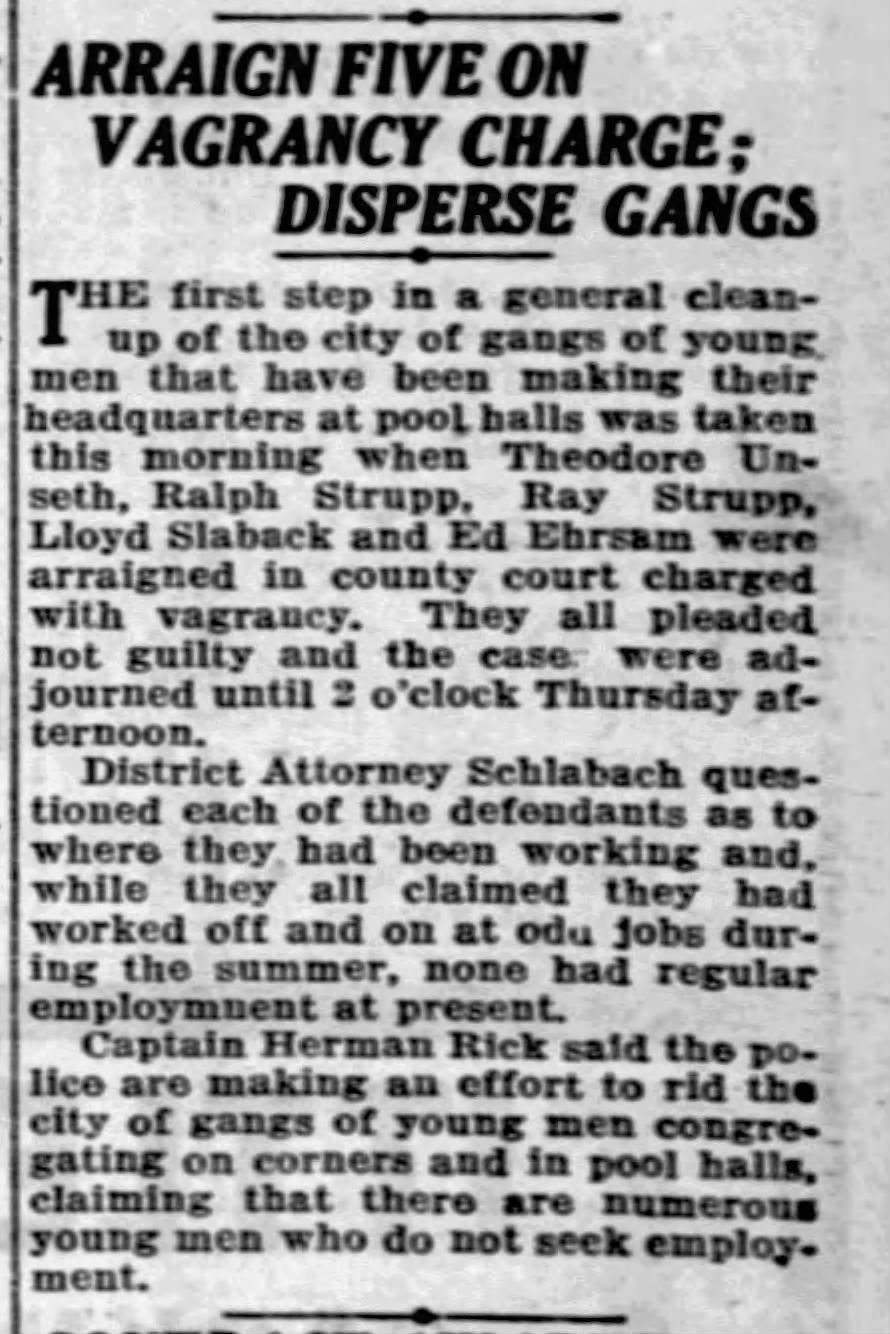
\includegraphics[width=0.6\linewidth,height=\textheight,keepaspectratio]{images/Akou05.jpg}

}

\caption{Article on the front page of the \emph{La Crosse Tribune},
November 5, 1929}

\end{figure}%

One day that fall, Lila arrived home from school and found her mother
and Aunt Hattie sitting at the table. They were drinking tea and it
looked like Hattie had been crying. Lila was surprised that they were
together because her mother didn't like Hattie very much. She didn't
think it was appropriate for a married woman to work outside the home.
(Hattie was not fond of Hazel either, but the Slabacks were the only
family she had in La Crosse.) ``Please go into the kitchen and peel the
potatoes,'' said her mother. Lila wanted to ask what was wrong, but she
knew it would only make her mother angry. Uncle Frank joined them for
dinner, but it was unusually quiet at the table. They talked about work
and Izro and Myron---they were expecting their first child. Aunt Hattie
had recently paid a visit to Myron's mother.

The next day when Veda was gathering rubbish from the house, she found a
newspaper folded to an article with Lloyd's name. She read it out loud
to Lila. Lila was confused. Lloyd was working for her father\ldots she
had seen him at their house. She asked Veda, ``What is vagrancy?'' Veda
said she didn't know, but it must be something bad if the police had
arrested him. No wonder Aunt Hattie had been crying.

Lila was still wondering about Lloyd when a stranger knocked on the door
one night during dinner.

``Can I help you?'' said her mother.

``Yes, I'm here to collect information for the census.''

She let the woman into the house and told Cecil to give up his seat.

The census taker said, ``This won't take long, but if you don't mind,
I'll sit with you and fill out the forms while you eat.'' She sat down
next to Lila and opened her book to a page that was nearly full of the
most beautiful handwriting, even nicer than Veda's. ``Mr.~Slaback, is
it? Could you kindly tell me your full name and your relationships to
these lovely young men and women?'' She had so many questions about
their names and ages, the value of their house, where their parents had
been born, and who was attending school. She asked the children to raise
their hands if they could read. Lila raised her hand with pride. This
was fun!

At the end, she asked Lila's father if he was employed and to describe
his line of work.

He said, ``Yes, I'm working. I do odd jobs around the neighborhood.''

What? Suddenly, Lila felt sick to her stomach. She remembered the
article about Lloyd; in the courtroom, he had claimed to be doing ``odd
jobs.'' Was her father going to be arrested too? Lyle was working for
her father's plastering business, but she noticed that the census taker
had recorded him as being ``in school.'' Lila said nothing and looked
around the table. Her mother and father did not seem concerned and did
not correct the census taker's mistake. Lila was relieved when the woman
thanked them and stood up to leave. Her mother followed her to the door
and said, ``Have a nice evening.''

There were plenty of good jobs available in La Crosse---at the rubber
mill, the iron foundry, the tobacco works, the MotoMeter factory, the
railroad---but John Slaback chafed at working for other people. He
didn't want to farm, but he didn't want other people telling him what to
do. His views on work boiled down to one statement: ``My ancestors
didn't come to this country to be slaves to the rich.'' His brother
Elmer had taught him how to plaster houses. It was satisfying work but
unpredictable. Sometimes, he would be so busy that Lila would barely see
him for weeks. At other times, there was barely any work, and their
budget would be stretched razor-thin. It was dangerous to ask for
anything during the lean times.

That night in bed, Lila asked Veda if their father was going to be
arrested for doing odd jobs.

``No, silly! Why would you ask that?''

Lila recounted how Lloyd had been doing ``odd jobs'' when he was
arrested by the police, but the newspaper said he was unemployed.

``Lloyd should be getting married instead of drinking and playing pool;
Daddy has been married for a long time.''

Lila was not entirely convinced. After a few minutes of letting the
matter swirl in her mind (what was ``pool,'' and why did it matter if he
was married?), she decided to trust her older sister's wisdom and
quickly fell asleep.

\section{Notes}\label{notes-9}

Slaback is not a very common name, so it was not too difficult for me to
find family members in databases of historic newspapers. This project
helped me learn how I'm related to every Slaback in La Crosse,
Wisconsin. The two family members mentioned in the newspaper most often
were Aunt Hattie (aspiring socialite) and her youngest son, Lloyd, who
spent most of his adult life in and out of prison; I imagine the
negative press was devastating to Aunt Hattie.

A distant relative that I connected with through
\href{https://www.ancestry.com/}{Ancestry.com} shared Lloyd's prison
record and letters that he exchanged with the Slaback family while
incarcerated. He had committed some petty crimes as a child, but those
records were expunged. The newspaper clipping describes what may or may
not have been his first crime as an adult. It appears to have been the
first time he was sentenced to prison.

There were two major factors in the 1920s and 1930s that led to moral
panic over ``gangs'' and criminal activity:

\begin{itemize}
\tightlist
\item
  the Great Migration (1915--1940) of Blacks into northern cities, and
\item
  the subversion of Prohibition laws, most infamously by Al Capone.
\end{itemize}

In ``sundown towns'' like La Crosse, the police focused their efforts on
lower- and working-class Whites. There was little tolerance for young
people who were unwilling (or unable) to work. Lloyd died long before I
was born, so I have no idea what he was like in real life. In this book,
I painted him as funny, handsome, and artistic, but also reckless. He
might have struggled in any period, but I wonder what he might have
accomplished with more tolerance and support. In letters from prison
near the end of his life, he expressed regret over his poor choices.

The 1930 Census is the first one where Lila Slaback appears in the
record. She was eight years old, and her family was living in the house
on Kane Street in La Crosse. Like the 1920 Census, enumerators were
asked to record information about literacy, education, and employment.
The question of whether the family owned a radio was new; the Slaback
family did own one. Lila's father, John, was recorded as working ``odd
jobs'' for hourly wages (not a salary).

For more information, see Deidre Bair\footnote{\citeproc{ref-bair2016a}{\emph{Al
  Capone: His Life, Legacy, and Legend} (New York: Doubleday, 2016)}.},
James Noble Gregory\footnote{\citeproc{ref-gregory2005a}{\emph{The
  Southern Diaspora: How the Great Migrations of Black and White
  Southerners Transformed America} (Chapel Hill: University of North
  Carolina Press, 2005)}.}, James C. Howell\footnote{\citeproc{ref-howell2015a}{\emph{The
  History of Street Gangs in the United States: Their Origins and
  Transformations} (Lanham, Maryland: Lexington Books, 2015)}.}, and
James W. Loewen\footnote{\citeproc{ref-loewen2018a}{\emph{Sundown Town:
  A Hidden Dimension of American Racism} (New York: New Press, 2018)}.}.

\bookmarksetup{startatroot}

\chapter{Chapter Nine}\label{chapter-nine}

In 1930 there were still eight people living in the house that Lila's
father had built on Kane Street, but it seemed unbearably quiet without
Theron and Izro. To cheer the family up, her father decided to buy a
radio. They made a place for it near the table so there would be plenty
of room to sit and listen. Lila's mother insisted that dinner time
should be for conversation, but otherwise their evenings were suddenly
filled with music, news reports, and serial programs. A quick favorite
for the whole family was ``Amos `n' Andy,'' which was about two friends
trying to make it in the big city. The show was funny, but it also made
them feel better about their problems---at least the Slabacks weren't
that stupid. While most of the programs on the radio were entertaining,
the news reporters were always very serious talking about the stock
market, unemployment, and President Hoover. Her father was not working
as much as he did the year before, but Lila thought her family was doing
fine. They had a house to live in and clothes to wear, and the shelves
in their basement were loaded with jars of food.

Theron built two wooden benches in the back of the truck so the whole
family could ride. During the summer, they started taking trips out into
the country. Although it was nice to spend time with their uncles,
aunts, and cousins (so many cousins that Lila could not keep track of
all their names), they could also do some work in exchange for food. A
few hours of weeding and picking might lead to crates of string beans,
baskets full of zucchini and tomatoes, or bushels of apples. Some of it
they ate right away, but Lila and Veda would help their mother preserve
the rest so they would have plenty of food for the winter. It was hot
work since the jars had to be sterilized and the vegetables needed to be
blanched in boiling water. Lila did not enjoy eating spinach, but she
loved watching it shrink in the heat---a whole basket of spinach could
fit into a single jar after the blanching process. When meat was
available, they turned it into sausages. The basement was cold, but salt
and spices would keep the meat from going bad regardless of the
temperature. One year---inspired by a neighbor from Germany---Lila's
mother decided to try making sauerkraut. Good lord! Lila thought the
smell was awful, like rotting eggs and sweaty socks. No matter how hard
she tried, Lila could not force herself to eat it, although her father
claimed that it was delicious with the sausage. They never made it
again.

One day, Uncle Frank and Aunt Hattie came to visit, and they decided to
take a walk out by the river. Veda and Lila were nervous and held hands
the entire time, but it was beautiful that day. The sky was stunningly
blue, and the banks were lush with milkweed, black-eyed Susans, and
Queen Anne's lace. As they walked along the coarse sand and rocks that
had been worn smooth by the river, Uncle Frank told a story about Lloyd.
Lila never forgot it because it was quite revealing about their family.

One day, when Lloyd was eleven years old, he went to a birthday party.
(``What was the name of that friend?'' he asked Aunt Hattie, who
shrugged and said she couldn't remember.) The party was held on a
steamboat, which was docked just two blocks away from their house on
State Street. Since it was hot in August, the party was held in the
evening---they were planning to take a ``moonlight cruise'' on the
river. One of his friends knocked on the door and they walked down to
the river together. Uncle Frank and Aunt Hattie had to go to work the
next day, so they were going to bed at their usual time. They told Lloyd
that they would leave the door unlocked: ``Have a good time, be careful,
and please be quiet when you get home.'' Lloyd promised that he would,
so everything seemed fine. When Aunt Hattie checked his bed in the
morning, however, Lloyd was not there. She woke up everyone in the
house. ``Frank\ldots Lloyd is missing! Kenneth\ldots have you seen your
brother?!'' She made everyone go outside to start knocking on doors.
After what seemed like forever (but was probably just a few minutes),
one of the neighbors told Aunt Hattie that her son had been at the same
party and invited Hattie to take a seat and wait for him. When William
(``Oh right, that was his name'') arrived in the sitting room, he said,
``The last time I saw Lloyd, he had fallen asleep on one of the
benches.''

Although Aunt Hattie had been running through all the worst-case
scenarios in her mind (maybe he drowned, maybe he was hit by a car!),
she realized now what had happened: Lloyd was a sound sleeper, and he
didn't wake up when the party was over. She thanked William and rushed
back home to call the steamboat company. They told her that the name of
the ship was The Capitol, currently on its way to Winona (on the
Minnesota side of the river). She thanked them and rushed out to send a
telegram to the Winona police: ``Lloyd Slaback, age 11, fell asleep on
The Capitol. Please send him back to La Crosse.'' Knowing that it would
take hours---maybe even a day---for Lloyd to return, Aunt Hattie and
Uncle Frank went off to work. He was home by the time they returned,
eating a sandwich and playing card games with Opal and Kenneth like
nothing had happened. The next day the story was in the newspaper: ``La
Crosse Boy Sleeps on Boat, Lands at Winona.'' Lila's mother said, ``My
goodness, that must have scared you half to death!''

Uncle Frank said, ``Not really\ldots all's well that ends well.''

Aunt Hattie blushed. ``I was horrified. Why did the reporters have to
write that story? The neighbors could not stop talking about it; they
said I was a bad mother for not waiting up. That incident was the reason
we left State Street and moved to the house on Copeland Avenue.''

For a few moments they walked in silence, and then Hazel changed the
topic to preparations for dinner.

Was Aunt Hattie really a bad mother? Lila and Veda exchanged nervous
glances and Veda gave Lila's hand a little squeeze. Her family wouldn't
forget about her and let her fall asleep on a steamboat\ldots would
they?

Lloyd was in the newspaper again that year. ``Well, I never\ldots{}''
said Lila's mother. They were all sitting at the table and Lila's father
had just finished reading the article out loud. Lloyd had threatened
someone with a loaded gun. He told the judge that he was too drunk to
remember what happened.

\$1,000 was an unimaginable amount of money. Lloyd was going to prison
for sure. Her father said, ``Lloyd is no longer welcome in this house. I
want all of you to stay away from him. Do you understand? Please tell me
that you do.''

Around the table there was a chorus of ``Yes, Father.''

Lyle's head was hanging down; he considered Lloyd a friend. When Lloyd
worked for their father, his jokes made the time go faster. Lloyd was as
funny as anyone on the radio.

John put his hand on Lyle's shoulder. ``Lyle, I also want you to
promise; Lloyd is drinking in public and spending time with the wrong
kind of people. He is nothing but a hoodlum.''

Lyle said, ``I understand\ldots I promise.''

Lila knew that going to prison was bad, but she was confused about why
the family was pushing him away. Did they have to punish him too?

\begin{figure}[H]

{\centering 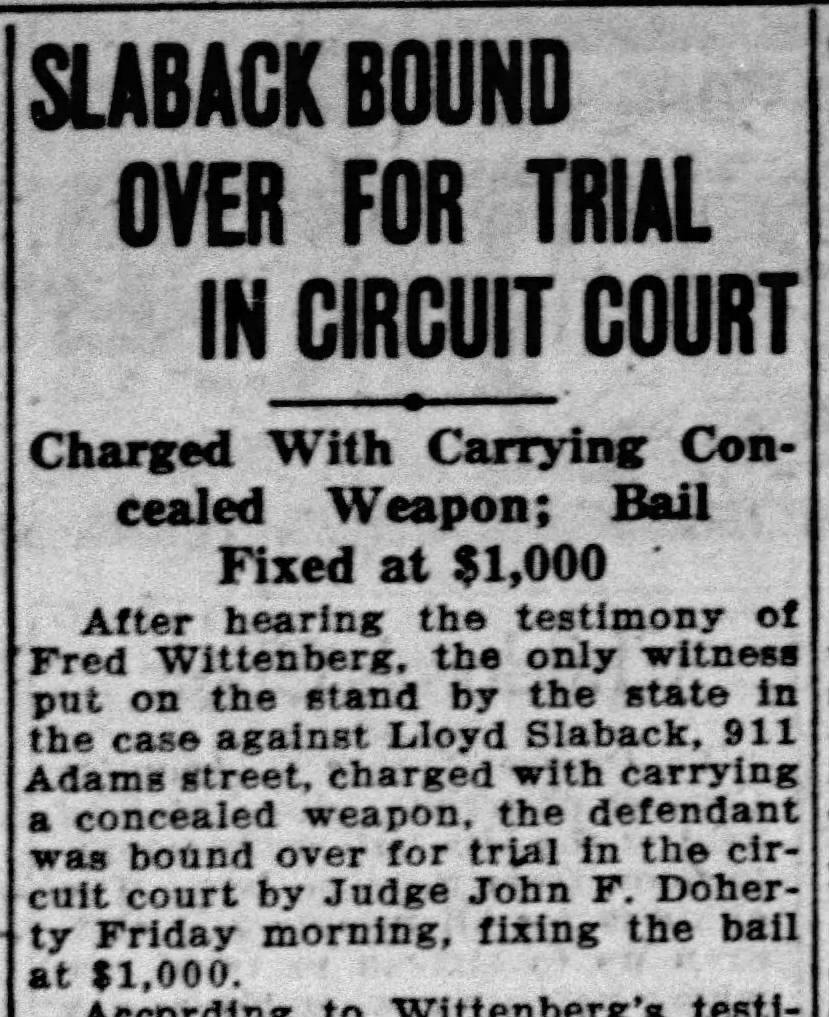
\includegraphics[width=0.7\linewidth,height=\textheight,keepaspectratio]{images/Akou06.jpg}

}

\caption{Page six of the \emph{La Crosse Tribune}, August 15, 1930}

\end{figure}%

\section{Notes}\label{notes-10}

Radio became a form of entertainment in the 1920s with the start of
broadcasting. Compared to films and theater productions, listening to
the radio was free (after the radio had been acquired) and did not
require travel or time outside the home. Radio programs could also be
enjoyed by the entire family simultaneously. Ownership expanded rapidly
in the 1920s and 1930s, even in working-class households. ``Amos `n'
Andy'' was an audio version of a minstrel show, featuring two White
voice actors who wildly exaggerated Black lifestyles and speech
patterns. The radio also delivered the news to listeners who could not
access newspapers.

Unlike many families in the Great Depression, the Slabacks were not
forced to move or split up. Their connections with family members who
were still farming (and their ability to preserve food by canning) may
have saved them. Both of my grandmothers knew how to can food as a life
skill and not as a hobby. My mother loved canned sauerkraut, but I
always hated the smell. When I was small, she canned peaches and
strawberry preserves for us to enjoy during the winter.

The winters are very long in Wisconsin. It can start snowing as early as
September and end as late as May. The long, cold, dark months are
depressing if you don't find new entertainment. Some people enjoy winter
sports like skiing, sledding, ice skating, and ice fishing. My father's
family was more interested in storytelling. The story of how Lloyd fell
asleep on a steamboat is exactly the kind of story they would have told
over and over---for fun, but also as a cautionary tale. Be careful.
Don't lose track of your friends. Don't scare your parents half to
death.

For more information, see Ethan Blue\footnote{\citeproc{ref-blue2012a}{\emph{Doing
  Time in the Depression: Everyday Life in Texas and California Prisons}
  (New York University Press, 2012)}.}, Tim Brooks\footnote{\citeproc{ref-brooks2019a}{\emph{The
  Blackface Minstrel Show in Mass Media: 20th Century Performances on
  Radio, Records, Film and Television} (Jefferson, North Carolina:
  McFarland, 2019)}.}, Russell Freedman\footnote{\citeproc{ref-freedman2005a}{\emph{Children
  of the Great Depression} (New York: Clarion Books, 2005)}.}, and
Michele Hilmes\footnote{\citeproc{ref-hilmes1997a}{\emph{Radio Voices:
  American Broadcasting, 1922--1952} (Minneapolis: University of
  Minnesota Press, 1997)}.}.

\bookmarksetup{startatroot}

\chapter{Chapter Ten}\label{chapter-ten}

In 1931, Cecil was in eighth grade, Veda was in fifth grade, and Lila
was in third grade at Roosevelt Elementary (named after Teddy Roosevelt,
not that communist). The Depression was taking a real toll on their
classmates. Some of the older students were dropping out of school to
work. Some had to leave La Crosse because their fathers were looking for
jobs in other cities. Veda's best friend, Minnie, was sent away to live
with her relatives, who still owned a farm in Vernon County. Although
Lila's parents did not seem too concerned about the whole situation,
worry began to follow her around like a hungry wolf. Lila was not the
worst student in her class, but she was also not one of the best. The
worry made it difficult to concentrate.

Aunt Hattie had stopped working as a waitress. She was in her fifties
and said that it was important for older people to let young people have
the jobs, but in truth it also gave her time to do charity work, throw
parties, and work on improving her reputation (which had been damaged by
the repeated stories in the newspaper about Lloyd). Theron's wife,
Borgny, was content to be a housewife and volunteered with the ``Bethel
Busy Bees,'' which made quilts, visited sick people in the hospital, and
organized fundraisers. Like Borgny, everyone in the group was a member
of Bethel Lutheran, the neighborhood church where she and Theron had
been married. Aunt Hattie was not a regular member of any church, but
she made that work to her advantage; it allowed her to host events in
her house for a variety of groups---one week it might be the LDS Ladies
Relief Society, the next week it could be Saint Wenceslaus or the
American Legion Auxiliary. She had a beautiful silver tea service and a
large set of matching china; as a hostess, she was always very gracious
and elegant. The constant rotation of groups kept ``Hattie Slaback'' on
everyone's mind as a model of generosity, but it also kept them from
getting too close and asking questions.

The house on Kane Street was full for Easter. Izro and Myron were
visiting for a few days so everyone could meet their son, LeRoy. Theron
and Borgny's daughter, Hilda Hazel, had the honor of being the very
first grandchild (and being named after her grandmother), but LeRoy had
been born during the same month. With blonde hair and blue eyes, the two
of them looked practically like twins. Lila was dismayed to realize that
she was no longer one of the ``children.'' She was allowed to do the
children's egg hunt in the park, but otherwise, it was like every other
day: beds to make, food to prepare, dishes to wash, and younger brothers
to keep out of trouble. Izro was a guest now and could not be expected
to help with the chores. Lila burst into silent tears when her mother
told her to sweep the floors. Hazel's patience had been wearing down all
day and Lila's tears were the last straw. ``You need to grow up,
Lila\ldots if you can't stop crying, you should go join the babies in
the other room.'' Izro found Lila in the kitchen washing dishes (still
crying) and hugged her. Lila had missed her so much.

Some people forget to eat when they're having a difficult time. Lila was
the opposite; the worry and sadness made her eat more. Being in the
kitchen all the time, it was easy to get extra food: a taste of the soup
to make sure it was done, a dinner roll that accidentally dropped on the
floor (hide the evidence!), or a few bites of dessert that one of the
younger children had failed to finish. It would have been a shame to
waste anything when so many people were going without. Like her teacher
said, it was her civic responsibility to do what she could. As a result,
Lila was getting a bit ``stout.'' When she looked in the mirror in the
bathroom, the only thing she admired was her eyes. They were like the
color of a quiet lake---dark green, with a hint of blue from the sky's
reflection. Her hair was light brown (so boring), her nose was a little
big, and her cheeks were way too big. Nobody else in her family had a
head shaped like a pumpkin.

\section{Notes}\label{notes-11}

My oldest child is dyslexic, a learning disability that clusters in
families. I have no idea if Lila was dyslexic, but she could have been.
Although she went to high school, she had fallen behind her peers that
were the same age. It appears that she did not graduate.

Hattie Slaback and Borgny Slaback were mentioned often in the \emph{La
Crosse Tribune}. Borgny was involved in the Bethel Busy Bees (associated
with Bethel Lutheran Church), but Hattie's pattern of involvement in
church and philanthropic groups was more scattered. She may have had a
difficult personality; she may have found it hard to explain her
independence or her son's prison record. I can only speculate.

This chapter reminds us of how much the Slaback family has changed. Lila
is no longer a little girl; she and her sister Veda are the only girls
in a house full of boys. The oldest grandchildren are close in age to
Lila's youngest brother. As an older mother who had raised many
children, I imagine that Lila's mother, Hazel, was quite exhausted.
Family stories have indicated to me that she did not have much patience
and was not a pleasant person to be around. As a child growing up in the
Great Depression, I imagine that Lila was dealing with a lot of fear and
grief without much support. Eating is one way to stuff emotions instead
of feeling them. Photographs show that Lila was overweight as a child,
but the rest of her family members were not.

For more information, see Joan Jacobs Brumberg\footnote{\citeproc{ref-brumberg2010a}{\emph{The
  Body Project: An Intimate History of American Girls} (New York: Knopf
  Doubleday, 2010)}.}, Julian G. Elliott and Elena L.
Grigorenko\footnote{\citeproc{ref-elliott2014a}{\emph{The Dyslexia
  Debate} (Cambridge University Press, 2014)}.}, and Lawrence Jacob
Friedman and Mark Douglas McGarvie, eds.\footnote{\citeproc{ref-mcgarvie2003a}{\emph{Charity,
  Philanthropy, and Civility in American History} (Cambridge University
  Press, 2003)}.}

\bookmarksetup{startatroot}

\chapter{Chapter Eleven}\label{chapter-eleven}

Inevitably, the ladies that Aunt Hattie was hosting began to make
inquiries---not so much about Lloyd, but about her membership (or lack
thereof) in a church. Where was she baptized? Where did she get married?
It was a real problem because Aunt Hattie and Uncle Frank only went to
church for weddings, funerals, and the occasional Christmas or Easter
service. One time, Hattie claimed that she was a Presbyterian---it was
the least controversial church she could think of. The Lutheran Church
was for the Norwegians and Germans, and the Catholic Church was for the
Irish. She had nothing against the Mormons, but she wasn't about to
claim that she was one of them; it would have been social suicide.

There was a Presbyterian church close to Lila's house. As a
demonstration of her faith, Aunt Hattie decided that Veda and Lila
should get baptized. Lila's mother pointed out that they had been
baptized in the local church when they were babies, but Hattie said it
was fine---it was common for people to get baptized again once they
joined a church in the city. She would buy new dresses for the girls;
afterward, they would have a lovely party at her house. Lila's parents
were not immediately convinced, but Veda desperately wanted to go
shopping with Aunt Hattie. She quietly asked their mother about it every
few days until finally, she threw up her hands and said, ``Fine, I guess
if you really want to get baptized again you can.''

On the day of the shopping trip, Uncle Frank arrived in his car to pick
up the girls. Aunt Hattie had invited their mother, but she decided that
she couldn't leave the younger boys without supervision. Veda and Lila
were secretly thrilled\ldots what an adventure! Uncle Frank drove them
downtown and dropped them off in front of Doerflingers, which was
Hattie's favorite department store. The savings from her years of work
allowed her to shop in ways that Hazel could not have imagined. Lila's
astonishment began when they went through the revolving door. Aunt
Hattie said, ``Come along dear.'' In her breathless state, Lila had
stopped walking and was blocking the door for other customers. The
building was five stories tall with an atrium in the middle; the roof
was supported by enormous columns that were clad with dark granite. It
was so highly polished that as they walked by, Lila could see a bit of
her reflection in the stone. Their footsteps echoed on the tile floor,
which had an elegant pattern of black and white squares.

The grand staircase at the far end was covered with emerald-green
carpet, but instead of heading for the stairs Aunt Hattie turned to the
left. There was a man patiently standing there, wearing a gray suit with
two rows of shiny gold buttons and gold trim around the collar, a flat
gray cap, and white gloves. He said, ``Which floor would you ladies like
to visit today?''

Without hesitation, Aunt Hattie said, ``Third floor please.''

He pushed a screen into a space behind the wall and said, ``Ladies
first.''

It was Lila's first ride in an elevator. There were mirrors all around
the walls, which made it appear as if they were standing in a crowd of
people who looked exactly like them. When Lila lifted the corner of her
dress, so did the rest of the girls. When she waved her hand, they all
waved back. She could have stayed in the elevator all day, but suddenly
there was a ``ding!'' and the man in the suit said, ``Third floor,
ladies; please watch your step.''

When the door opened, it appeared that they had just entered the sitting
room for a very fancy house. It had a matching set of sofas and chairs
covered in velvet, a large oriental rug, an enormous radio, a crystal
chandelier, and a low table set up for tea with a silver tea service and
various colors of china. The back wall was filled with bookcases. Lila
could not imagine that anyone would be able to fill so many shelves, but
the room was impressive. It was a teaser for the floor above, which was
filled with furniture, linens, cookware, and china. Veda and Lila
followed Aunt Hattie past the men's clothing, shoes, and hats, around
the back to the children's section which contained a mixture of clothing
for boys and girls. There were also toys---china dolls with curly hair
and frilly dresses, miniature tea sets, a rocking horse with a mane and
a tail made of real horsehair---but Lila knew better than to touch
anything. They were here to shop for dresses for the baptism, not for
toys.

A woman approached them and said, ``May I help you with anything today,
ladies?'' Similar to the man who helped with the elevator, she was also
wearing gray, but instead of gold buttons, her dress was accented with a
crisp white collar and cuffs.

Aunt Hattie told her, ``Yes dear, we're here to find dresses.'' To
clarify ``for the girls,'' she put her arm behind Veda and gently nudged
her forward.

The woman reached out for Veda's hand and said, ``Oh, aren't you a
beauty! I know just the dress for you.'' After pulling out some dresses
that Veda and Lila could try on, the woman indicated that they should
follow her to the back. The fitting room was large enough to hold all
four of them. It was painted dark green and there were two large mirrors
hanging together in one corner.

Aunt Hattie sat down on the elegant sofa and said, ``You can take off
your shoes and dresses but leave on your panties and undershirt.''
Although Aunt Hattie behaved like they were doing the most natural thing
in the world, Lila found it unsettling to take off her clothes in front
of a stranger.

The saleswoman held out a beautiful light blue dress and said to Veda,
``I think you should try this one on first; the color will be lovely
with your eyes.''

Veda blushed and said, ``I like that one too.''

Aunt Hattie insisted that she try on several dresses (just to be sure),
but everyone agreed that the blue one was the best. Veda looked
stunning---like a young woman instead of a child. The fluttery sleeves
and full skirt accented her tiny waist. Aunt Hattie said, ``We'll need
to get you some nice shoes to go with that.''

While she was still trying on dresses, the saleswoman held one out for
Lila. It was white with red polka dots and a red sash. ``I think this
one will look gorgeous on you.'' Much to Lila's dismay, however, the
dress would not fit over her hips.

Aunt Hattie said, ``Don't pull on it, Lila, it's alright if the dress
doesn't fit.''

The saleswoman added, ``Don't worry, dear. I'll find you a larger
size.'' The woman left the room and came back with five more.
``Unfortunately, I don't have a larger size for the red-and-white dress,
but here are some others that I think you will like.'' None of those
dresses fit either. Lila was starting to feel very embarrassed. Why did
trying on dresses have to be so easy for Veda and so difficult for her?
When one of the dresses finally fit (it was yellow and made Lila feel
like a giant goldfinch), she put on a big smile and said, ``Oh, I love
this one.''

The saleswoman could not disguise her sigh of relief. ``You look
beautiful, dear. I'm so happy that one works for you.'' She turned to
Aunt Hattie and said, ``Is there anything else you need today, or shall
I take your packages downstairs?''

Before heading to another shop to look for shoes, Aunt Hattie took them
to the tearoom on the second floor so they could have lunch. A waitress
(who, Lila observed, was wearing the same gray dress with a white apron)
brought them a tray with tea, milk, sugar, little sandwiches cut into
triangles, a bowl of fruit, and a plate of cookies. Some of the
sandwiches were filled with egg salad (delicious); others were filled
with cream cheese and had a slice of cucumber on top. The cookies were
dark pink and filled with cream. The first one was so good, but when
Lila reached for one more Aunt Hattie said, ``Do you really think you
should be eating that?'' Lila pulled her hand back and was silent for
the rest of the meal.

A few weeks later, Aunt Hattie invited them back to her house for tea.
Veda was thrilled. Aunt Hattie was so glamorous. Veda wanted to live in
a house like hers someday, with a modern stove and washing machine and
big beautiful sitting room to entertain guests. After they had their
first cup of tea Aunt Hattie said, ``Veda\ldots on top of the dresser in
my bedroom is a big jewelry box. Why don't you go pick something out to
keep as a present? A young lady like you should have an elegant piece of
jewelry to wear to parties.''

Veda's eyes lit up with excitement and she said, ``Really?''

Aunt Hattie smiled and nodded her head. She said, ``Go on, dear.'' Once
she was out of earshot, Aunt Hattie turned to Lila and said, ``Your
sister is such a beautiful girl. In just a few years she's going to be
very attractive as a bride.''

Why was Aunt Hattie telling her this? Lila knew that Veda was beautiful,
but it was hard to imagine her as a grown-up.

``As for you\ldots{}'' Aunt Hattie continued, ``You need to pay more
attention to your diet. Stout girls do not get invited to parties.''

Lila was so embarrassed. She had no idea what to say. She looked down
into her empty teacup and resolved to stay away from Aunt Hattie.

\section{Notes}\label{notes-12}

The Slabacks were not very religious. It took me months to figure out
the denomination of the church that was next to her father's farm in
Crawford County (Methodist). The only evidence that Lila Slaback went to
church in La Crosse is her baptismal record. This is a mystery to me
since the church for her baptism was Presbyterian. It is not uncommon
for Christians in the US to attend church only for Easter and Christmas.

Doerflingers was a real department store in La Crosse in the early
1900s. Although I could only find images of the exterior, I used images
of other department stores from the same time to imagine what the inside
would have looked like. In the 1930s, only the most luxurious stores in
the Midwest had elevators. They were more dangerous and difficult to
operate than elevators today, so buildings hired operators to open and
close the doors and direct customers. The staff in grand department
stores wore uniforms similar to the attendants in theaters and hotels. I
have no idea when Lila rode an elevator for the first time, but I
remember being fascinated by them as a child. I also loved three-way
mirrors due to the way they created ``many girls'' when I looked in
them. In the early 1900s, buying ready-to-wear was still a novelty,
especially for working-class girls and women in the Midwest. (It was
more common for men.)

One of the problems with mass-manufactured clothing is that it doesn't
fit everyone. Shopping can be a fun adventure when the clothes fit. If
they don't fit, shopping can foster (and reinforce) feelings of
body-consciousness and embarrassment. Before ``plus-size'' became a
dominant term in the fashion industry, young women who were too large
for standard sizes were referred to as ``stout.'' By rewarding Veda and
shaming Lila, Aunt Hattie (whether intentionally or not) was driving a
wedge between them. This is foreshadowing for future chapters.

For more information, see the author\footnote{\citeproc{ref-akou2024a}{\emph{On
  the Job: A History of American Work Uniforms} (Oxford: Bloomsbury
  Academic, 2024)}.}, Lauren Downing Peters\footnote{\citeproc{ref-peters2023a}{\emph{Fashion
  Before Plus-Size: Bodies, Bias, and the Birth of an Industry} (Oxford:
  Bloomsbury Academic, 2023)}.}, and Jan Whitaker\footnote{\citeproc{ref-whitaker2006a}{\emph{Service
  and Style} (New York: St. Martin's Press, 2006)}.}.

\bookmarksetup{startatroot}

\chapter{Chapter Twelve}\label{chapter-twelve}

A few months after he started driving the truck for a living, Theron
joined the Teamsters. He didn't really understand the purpose of a
union, but it gave him access to steady and better-paying delivery jobs.
The dues were a small price to pay. During a strike in 1932, he felt
lucky to find a different job right away. With a wife, a daughter and
Borgny pregnant again, he couldn't afford to be out of work. La Crosse
County was building a new highway and needed drivers to haul gravel. He
was also perpetually grateful to have the use of his father's truck. He
didn't have much of a talent for building and hated the idea of working
in a factory, but driving was actually fun. It barely felt like work at
all.

Sometimes, when he picked up the truck in the morning, he liked to spend
some time at his parents' house, chatting and having breakfast. Lila
noticed that her parents were different when he came to visit---softer,
more patient and more likely to smile. Their affection for their
first-born son was obvious. Lila was sure that her parents loved all
their children, but they had their favorites. Hazel expected Lila to be
quiet and helpful at all times (and frequently criticized her for
failing to meet her impossibly high standards), but her younger
brothers, Earl and Looy, were quite spoiled. They never had to mind the
children since they were the youngest. Her older brothers had some
responsibilities, but they were much smaller than Veda and Lila's. Cecil
was responsible for mowing the lawn and shoveling coal into the furnace.
Lyle took the rubbish to the curb for collection days and helped his
father with repairs around the house. When there was snow, Theron did
the shoveling around the sidewalk and driveway so he could get the truck
out of the garage. Veda and Lila did everything else. Earl was already
nine years old, but he didn't have any regular chores. It must be nice
being a boy, thought Lila.

One Friday morning in November, Theron (as usual) was over for
breakfast. Since it was a school day, everyone except Looy was awake. As
soon as Earl finished eating, he went outside to play. Veda was reading
a book. Lila preferred to eat slowly and enjoy her food, knowing that
less-pleasant activities were waiting\ldots clearing the dishes and
walking to school. When Theron finished eating, he said, ``I guess I
better be going now.'' He gave their mother a kiss on the cheek and
headed through the kitchen to the back door.

They heard the truck starting, and Lila's mother sighed. ``This weekend
I want to give the house a thorough cleaning. When you get home from
school, please gather the towels and dirty laundry and then we'll strip
the beds in the morning.''

Lila started clearing the dishes and said, ``Yes, ma'am.'' Her friend
Nora was having a birthday party on Saturday, but she knew it was no use
asking to go. Her mother would never change her plans once her mind was
made up.

A few moments later there was a loud knock at the front door. ``Who
could be calling at this hour?'' said her mother. She went to the front
door and Lila followed; anything was better than cleaning.

Their neighbor, Mrs.~Bay, was standing there in her robe and said,
``There was an accident! You need to come with me right away!''

Veda set her book down and they all went outside. At the end of the
block, there was a small cluster of people. Theron was kneeling in the
street, rocking back and forth. Lyle was standing next to him looking
white as a ghost. Their mother was running now, saying,
``Theron\ldots what happened\ldots are you alright??''

One of the neighbors stopped her and said, ``Mrs.~Slaback, your son Earl
has been hurt. My husband took him to St.~Francis Hospital.''

Mr.~Bay pulled up in his car and said, ``Let me give you a ride,
Mrs.~Slaback.''

Their mother turned and told Lila, ``Go back to the house and wait for
me there. I'll be back as soon as I can.''

Lila wanted to stay and figure out what was going on, but like a good
girl, she said, ``Yes, mother'' and turned back around.

It was so quiet inside the house. For a few minutes, Veda and Lila just
stood there, not making a sound. Although it was a school day, their
mother's instructions had been clear: wait inside the house. Finally,
Veda said, ``I guess I better check on Looy. Why don't you clear and
wash the dishes?'' Lila had never been so grateful for chores. Her mind
was racing, but it was good having something familiar and productive to
do. As the hours passed with no word from their mother (or even their
brothers\ldots where was everyone?), Veda and Lila did all the chores
they could think of. They made the beds and swept the floors. They
played games with Looy and made two batches of snickerdoodles. There was
a roast thawing for dinner, so after lunch, they cut up some carrots and
potatoes and put everything to bake in the big roasting pan. They even
cleaned the bathtub and toilet and took all of the dirty laundry to the
basement. The roast smelled delicious. Lila was getting hungry, but Veda
said they should wait until everyone was home before eating dinner. Lila
reluctantly agreed and set the table.

The sun was setting by the time they heard the truck pulling into the
garage. Cecil was the first one into the house. He said nothing and went
straight to the bathroom. Lyle also went upstairs without a word. What
was going on? Their mother walked in the door. Her eyes were red; it was
clear that she had been crying. Their father was right behind her and
said, ``Girls\ldots please go to the living room; I'll be with you in a
minute.'' Veda sat down on one of the chairs and picked up the book that
she had been reading that morning. Lila also sat down and was idly
swinging her legs. She wasn't sure what else to do.

When their father entered the room, Lila thought he looked older,
somehow, like ten years had gone by in one day. He said, ``Girls, I need
to tell you something. Your brother Earl is dead.''

What? Veda's jaw dropped open; Lila felt like she had been punched in
the stomach. They all sat there for a few moments in silence. What do
you say to that kind of news? Finally, Veda asked, ``How did it
happen?''

Their father responded that he wasn't sure; Lyle had seen the accident
but was still in shock. Theron was last seen giving a statement to a
police officer; he didn't go to the hospital. Cecil wasn't sure what had
happened either. Looy spoke up and said, ``Where is Earl? What is
`dead'?'' Their father put his hands over his face to hide his tears,
but his shoulders and back were shaking from the sobs.

\begin{figure}[H]

{\centering 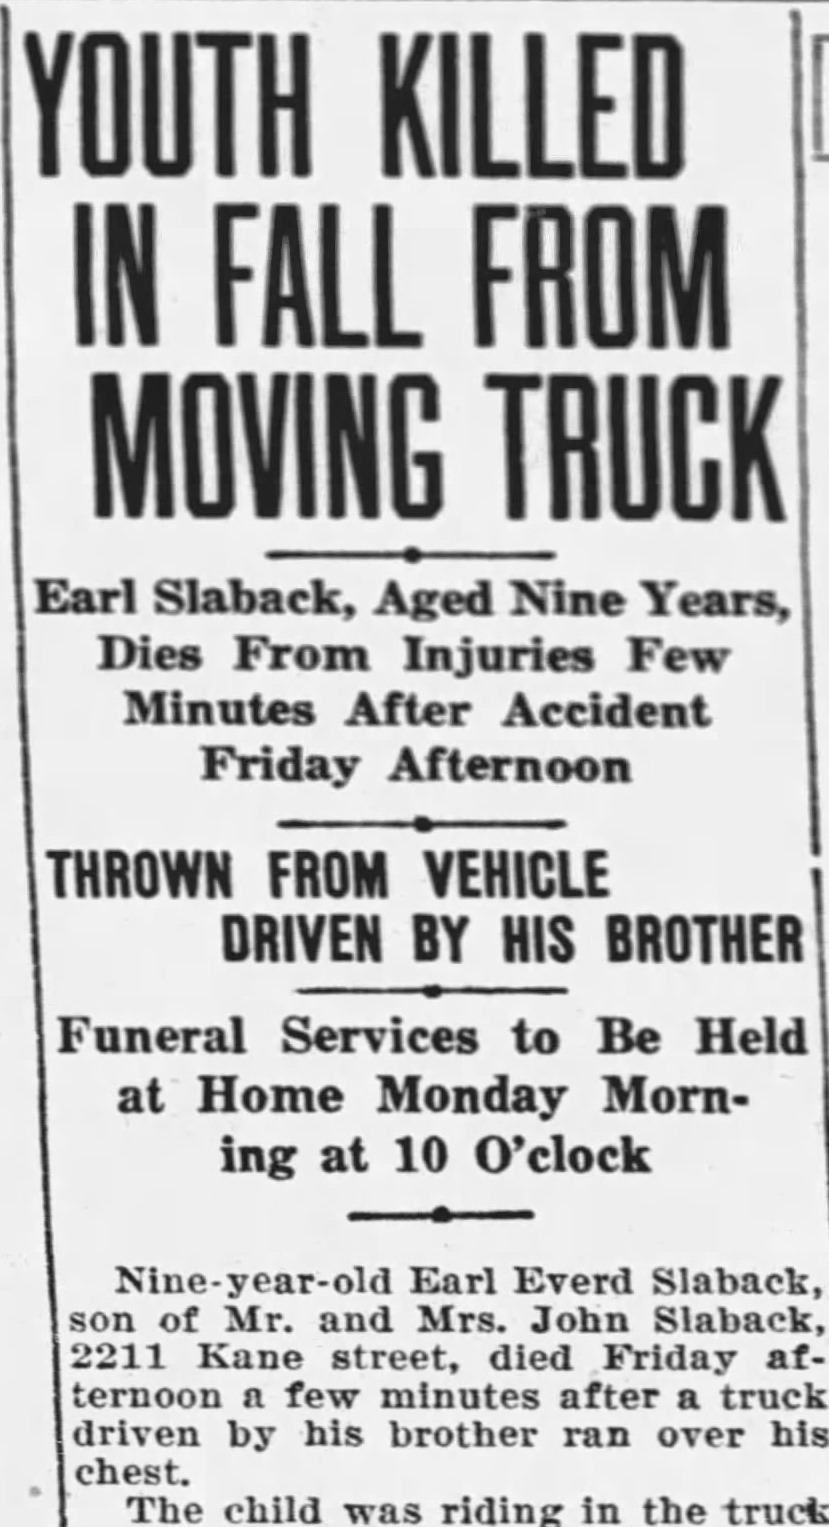
\includegraphics[width=0.6\linewidth,height=\textheight,keepaspectratio]{images/Akou07cropped.jpg}

}

\caption{Front page of the \emph{La Crosse Tribune}, November 4, 1933}

\end{figure}%

Lila knew what death was. Earl was an annoying little brother, but Lila
didn't want him to die. Who was with him when it happened? Would there
be a coffin? One of her classmates had died the previous year from
scarlet fever. His family was too poor to have a coffin, so they buried
him in a canvas bag. Although some people had stayed away (out of fear
that the body might still be contagious), Lila had gone to the funeral.
Everyone who attended went through a line so they could see Edward one
last time and talk to his family. His mother had given her a hug and a
kiss on the head. Lila knew that everyone died eventually, but losing a
child was the worst. Just like Earl, Edward had been perfectly healthy
and normal. He was eating, going to school, playing games with his
friends, and then boom. Gone forever.

The next day, the story made the front page of the newspaper. It said
that Earl had fallen out of the truck, which ran over his chest. He was
able to get up and had started walking back to the house, but he was
dead from internal injuries by the time Mr.~Bay arrived at the hospital.

\section{Notes}\label{notes-13}

Census records show that in 1930, Theron Slaback was
twenty-one-years-old and working as a ``boiler washer'' on the steam
railroad. His wife, Borgny, had just given birth to their first child
and they were living in a house a few blocks away from the Slaback house
on Kane Street. By 1940, he had shifted to working as a truck driver,
which paid better and was more independent.

My father grew up in a house with six sisters and two boys and has often
described how much housework the girls were expected to do. His main
chore was shoveling coal into the furnace.

I used census records to find the names of people who lived in the same
neighborhood as the Slaback family. As I combed through articles from
the \emph{La Crosse Tribune} in the 1930s, I was shocked at how common
it was to be injured or killed in an automobile accident. I had no idea
that Theron had accidentally killed his younger brother, Earl. What a
devasting event that must have been for the family. The family did not
have a telephone, so I imagine it would have been both boring and
terrifying for Lila and Veda to wait for news about Earl. Their efforts
to do the chores remind us what they are capable of, which foreshadows
the next few chapters.

For more information, see Peter D. Norton\footnote{\citeproc{ref-norton2011a}{\emph{Fighting
  Traffic: The Dawn of the Motor Age in the American City} (Boston: MIT
  Press, 2011)}.} and Susan Strasser\footnote{\citeproc{ref-strasser1982a}{\emph{Never
  Done: A History of American Housework} (New York: Pantheon Books,
  1982)}.}.

\bookmarksetup{startatroot}

\chapter{Chapter Thirteen}\label{chapter-thirteen}

Outside of the house on Kane Street, life continued as normal. Lila
heard later that Nora had her birthday party. Of course she did. Her
little brother was still perfectly alive. Veda and Lila had already
cleaned most of the house, so to pass the time they listened to the
radio and played with Looy. Their mother disappeared into her bedroom on
Friday evening and didn't reappear until Monday morning---not even for
meals. Lila thought she must be starving but knew better than to
comment. Even in good times, her questions were usually ignored or met
with anger. Everyone was so quiet. Lyle and her father left for a while
to do some work since they would not be able to work on Monday. Cecil
stayed upstairs for most of the weekend.

On Monday morning, Lila woke up to find that several of the neighbors
were getting the house ready for the funeral. They brought extra chairs
and platters of food; Lila had never seen the table so loaded. She was
combing her hair and putting on her clothes (regretfully, she noted that
the yellow dress barely fit) when the undertaker arrived. He set up a
small platform near the front door and then a few of the men helped
carry in the coffin. Lila was relieved to see that her brother would
have a proper burial, but she was also curious. What did he look like in
there? Shortly before the service, the reverend arrived and opened the
top half of the coffin. As soon as he left the room to speak with her
parents, Lila went up to the coffin to take a peek. Earl was wearing the
clothes he usually wore to school. She noticed that two of the buttons
on his shirt were broken, but otherwise there was nothing out of the
ordinary; Earl looked like he was sleeping. Veda was standing beside
her, quietly crying, Lila was usually the more emotional one, but on
this particular morning, she was surprised to feel nothing. She wasn't
angry or frightened or even sad. Maybe, she thought, this is what it
meant to be ``in shock.'' Lila touched Earl's hand like she had done
many times before, but it was so cold and stiff---so lifeless---that she
quickly pulled her hand back.

By ten o'clock the house was filled. Many people were standing. Some had
to stand in the kitchen or outside; there wasn't enough room for
everyone. Lila recognized many of Earl's classmates. Aunt Hattie and
Uncle Frank were sitting in front with her parents. Theron and Izro were
also in front. Lila had not noticed when Izro arrived. Since there would
be another service before the burial in Crawford County, the reverend
did not speak for long. When the line formed so everyone could see Earl
and talk with her parents, Lila joined the line for food. The neighbors
had put together an impressive spread. In addition to a huge plate of
ham sandwiches, there were bowls of vegetables, bowls of pickles, trays
of cookies, a basket of apples, and numerous pots of coffee and tea.
When Lila bit into one of the sandwiches, she was surprised to find that
it had a generous slab of butter; it was not what she had expected, but
it was good. She went back for a second helping (and then a third
helping) and nobody said a word.

By noon, most of the visitors were gone. The adults were standing near
the front door, having a discussion. Aunt Hattie said, ``Well it's
settled then; Hazel and John will ride with us and Lyle will drive the
children.'' It was time for the men to carry Earl to the truck. One of
the neighbors, Mrs.~Christiansen, was still standing over the coffin.
Her husband and son had been killed in an automobile accident just a few
weeks earlier. Lila was surprised that she was there. The reverend put
his hand on her shoulder and said, ``Mrs.~Christiansen, can I walk you
back to your house?'' She nodded and started moving towards the front
door. Theron softly closed the lid as the men lifted the coffin off the
pedestal. They carried it to the truck and placed it in the middle of
the flatbed. As Lila climbed in and sat down, she thought about their
most recent trip to Crawford County. Just two weeks ago, the truck had
been filled with bushels of apples from Aunt Stella's farm. Today,
instead of weeding and picking vegetables, they were on their way to put
Earl in the ground. It was so desperately strange and wrong.

Earl was the first member of the family to die in La Crosse. To Lila's
parents, it seemed natural that he should be buried with the rest of the
family in Crawford County. To Lila, it was yet another insult. They were
going to leave Earl out there, all alone, and go back to La Crosse like
nothing ever happened. There had been frost on the ground that morning,
but by the time they arrived at the church next to her grandparent's
farm, it was becoming a beautiful day. The sun was warm, and the air was
rich with the smell of fallen leaves. The snow could start falling any
day now; every last bit of sunshine was a gift. Only five years had
passed since the family moved to La Crosse, however, Lila barely
remembered the church. The building was already packed when they
arrived. As they filed into the first pew, Theron, Lyle, Cecil, and her
father carried Earl's coffin to the front.

``Today, we are here to bid farewell to our beloved brother, son,
nephew, and grandson, who was called to Heaven at such a tender
age\ldots.'' Lila barely heard the rest of the service. She could feel
the weight of her body sitting on the bench, her lungs filling and
releasing the air, her heart pounding in her chest, and her toes
pressing into her shoes (which were far too small, but it would be
months before her family could afford another pair). Physically, she was
very much alive, but it seemed like her feelings had died the same day
as her brother. Veda's handkerchief was already damp with her tears.
Lila's handkerchief was sitting in her pocket, unused. All around the
church, she could hear people sniffling and quietly crying---their grief
was like a weight pressing on her shoulders and chest. She did not feel
like she could join them; in her mind was a phrase that she had heard
many times: ``Big girls don't cry.'' Earl was her brother, but she felt
like a stranger looking at the scene through a glass window.

After the burial, there was another dinner. The food was delicious and
there was so much of it: roasted chicken, smoked ham, baked potatoes
with butter and sour cream, pumpkin pies, apple pies, bowls of pickles,
and a giant block of cheddar cheese. For a little while she played with
her younger cousins, but the pinched look of disapproval on Aunt
Hattie's face ended the fun. She was supposed to be in mourning like a
proper young lady. It felt like another injustice. She tried so hard to
be good, but Aunt Hattie never seemed to notice her good behavior. By
the time they drove home, it was already getting dark.

\section{Notes}\label{notes-14}

I was younger than Lila the first time I went to a funeral, but I
distinctly remember when my great-grandfather died. I was nine years
old. During the viewing of his casket (where family and guests view the
body one last time), one of my younger cousins asked if he could touch
my great-grandfather's hand. I was surprised by that request but also
curious, so when I thought nobody was looking, I touched my
great-grandfather's hand. His skin was soft and very cold. Like Lila, I
quickly pulled my hand back.

``Funeral sandwiches'' are common in the United States. My experience,
growing up in northern Wisconsin, is that they consist of white bread
with ham and a lot of butter. In the South, funeral sandwiches are also
known as ``party sandwiches'' and can be served for any occasion (happy
or sad) where a large group of people is expected. For working-class
families, the closer you go to the source of the food (i.e., the farm),
the more plentiful it becomes.

What place did John and Hazel Slaback think of as home? Since they
decided to bury their son in Crawford County (where they had both grown
up), I suspect they were not feeling completely settled in La Crosse.
I'm not sure they ever planned to move back or could have afforded to,
but feeling like a place is ``home'' is more connected to the heart than
reality. For Lila---who moved to La Crosse as a small child---I imagine
the city always felt like home. This created a distance between her and
her parents, but I'm not sure they would have recognized it. If they
ever did, it was probably too late to benefit Lila. Despite being part
of a large family, Lila was generally on her own to find her way as a
city girl.

For more information, see Candi K. Cann\footnote{\citeproc{ref-cann2018a}{\emph{Dying
  to Eat: Cross-Cultural Perspectives on Food, Death, and the Afterlife}
  (Lexington: University Press of Kentucky, 2018)}.}, Kenneth J. Doka,
ed.\footnote{\citeproc{ref-doka2014a}{\emph{Children Mourning, Mourning
  Children} (Abingdon, United Kingdom: Taylor \& Francis, 2014)}.}, and
Kate Sweeney\footnote{\citeproc{ref-sweeney2014a}{\emph{American
  Afterlife: Encounters in the Customs of Mourning} (Athens: University
  of Georgia Press, 2014)}.}.

\bookmarksetup{startatroot}

\chapter{Chapter Fourteen}\label{chapter-fourteen}

The day of Earl's funeral was the day everyone's childhood came to an
end. Hazel and John were both crushed by the loss of their son. For
John, it called his choices into question, especially the decision he
had made to stop farming and move the family into the city. Would Earl
still be alive if they had stayed in Crawford County? There were dangers
everywhere, but the city was filled with vehicles and that was the cause
of Earl's death. Although everyone knew that the accident was not
Theron's fault, Hazel quietly blamed him. He should have looked for Earl
before driving off. What had possessed him to be so careless? Theron
blamed himself too, but Lila would not know that until years later. He
stopped coming by for breakfast and started parking the truck on the
street in front of his own house instead of pulling it into the garage.
It seemed like their father barely noticed; a few weeks after the
funeral, he stopped working. He didn't have the energy. Lyle took over
the business, and Cecil dropped out of school to help.

For a few weeks after the funeral, the family had a steady stream of
visitors; friends and neighbors stopping by to check on them, often with
a casserole. (Many of the dishes were good, but Lila would never think
about casserole the same way again). Viola and Myrtle came to visit with
their mother, who made a beautiful sour cream and raisin pie. Although
her parents didn't know them very well---Myrtle was in the grade between
Lila and Earl---it was a good day in the Slaback house when they
visited. Everyone was dressed; nobody was crying or yelling. When
Mrs.~Johnson said that she was ``so sorry about what happened'' and to
let her know if there was anything she could do to help, her mother
said, ``Thank you so much for your kindness. We're managing.'' Lila knew
that was not the truth, but her mother was too proud to ask for help. If
someone offered something specific, (``Let me bring some extra jars of
pickles for your pantry''), she wouldn't say no. Everything else, they
would take care of themselves. It was an unspoken rule. Eventually the
visits stopped, and the offers of help faded away. Everyone assumed that
the Slabacks must be ``doing fine'' if they were not asking for
anything.

Truthfully, they were not doing so fine. When their mother started
drinking (which was easy now that Prohibition was over), Veda became the
de facto head of the household. If Looy had been younger, she might have
dropped out of school to take care of him. Thankfully, Looy was just old
enough to start attending school in January. Veda was nearly fourteen
and could do everything necessary to keep the household running,
including the laundry, taking care of the garden, preserving food for
the winter, and making sure that Lila and Looy were going to school.
Lila took charge of making the beds, cleaning the bathroom, and cooking
breakfast for everyone. Their mother usually made oatmeal, but Lila
decided that toast would be easier. She could make bread for the whole
week and toast a whole tray of slices under the broiler. With some jam,
tea, and hard-boiled eggs, it would be a complete and nearly instant
breakfast for the whole family. Nobody said a word about the change. A
lot of things were changing.

Underlying the emotional depression going on in their house was the
Great Depression. Lila could barely stand listening to the news on the
radio---strikes, soup lines, banks going out of business, organized
crime, unemployment, terrible dust storms in Kansas---there seemed to be
no end in sight to the difficulties the whole country was having.
Although Aunt Hattie had worked as a waitress and her daughter worked at
the Electric Auto-Lite factory, Lila realized that married women were
not ``supposed'' to work outside of the home. Her teachers said that if
every family had just one job per household, the problem of unemployment
would be solved. Married women should stay home to take care of the
cleaning and children and leave jobs to the men. Lila spent many hours
thinking about it while she did chores. Her parents were married, but at
the moment neither one was working. Did ``odd jobs'' count as jobs? If
so, there were two people working in her house (Lyle and Cecil), but
they were supporting seven people. Shouldn't there be some kind of
allowance for the size of the family? Did farming count? Lila wished
that chores counted as jobs. She would be rich if she could get paid for
doing housework.

Sometimes she fantasized about what it would be like to be rich. She
would have a big fancy house---like the gray-and-white one next to the
streetcar line heading downtown, which had a big tower over the porch
(just like a castle!)---and it would have stained glass windows and
beautiful rugs and feather pillows. She would have three cats
(Annabelle, Izro, and Nora), and she would hire boys and girls from poor
families to do all the chores---that way they could afford to stay in
the city and not leave for somewhere else. It was hard saying goodbye to
friends. As a rich person, she would never have to do laundry again and
could eat cake and ice cream every day for dinner. She would buy all of
her clothes at Doerflingers and tell the elevator man, ``Third floor,
please,'' like it was the most natural thing in the world. She would
have a car and Veda could be her ``show-fur.'' Lila giggled thinking
about that one. What a silly word for someone who drives a car for other
people. One day she was so busy fantasizing about being rich that she
burned the toast. Nobody said anything at breakfast, but internally she
kicked herself for the rest of the week. She would have to be more
careful about getting lost in her thoughts.

\section{Notes}\label{notes-15}

In northern Wisconsin, casserole---also known as ``hot dish''---is a
classic food to give a family that is grieving, recovering, or
overwhelmed with life. While it's possible to make it and eat it at
home, it's more common to give it away. Casseroles are designed to be
inoffensive and easy for the recipient to reheat. Sour cream and raisin
pie is a classic dairy-based dessert from Wisconsin that my father's
mother used to make for Easter. This scene is the second time Viola and
Myrtle appear in the book. It gives us insight into the mindset of the
Johnson family and how they were willing to offer support to
less-fortunate neighbors.

I can only imagine how the Slaback family's process of grieving must
have been compounded by the struggles of the Great Depression. One of my
father's aunts (who was born in 1921, the year before Lila) talked about
the Depression from time to time when she visited our home on Friday
evenings to play cards and chat with my mother. One night she voiced the
idea (expressed in this chapter by Lila's teacher) that there should be
``only one job per household.'' As a young woman she had worked as a
teacher but had quit when she got married. That was the social
expectation at the time, for women to be homemakers and not work outside
of the home.

In the 1930 US Census, enumerators were instructed to use one of the
columns to identify the ``head of family'' and ``homemaker'' for all
single-family dwellings:

\begin{quote}
\begin{enumerate}
\def\labelenumi{\arabic{enumi}.}
\setcounter{enumi}{131}
\tightlist
\item
  Home-maker.---Column 6 is to be used also to indicate which member of
  the family is the ``home-maker,'' that is, which one is responsible
  for the care of the home and family. After the word ``wife,''
  ``mother,'' or other term showing the relationship of the person to
  the head of the family, add the letter ``H,'' thus: ``Wife---H.'' Only
  one person in each family should receive this designation.
\end{enumerate}
\end{quote}

Lila might have coped by daydreaming. In this chapter, she dreams what
it would be like to be rich and to take care of the people who are
important to her (like her classmates, friends, and her sister, Veda).
It gives her relief from reality, but it also causes some trouble and
disconnection in her real life. This foreshadows events to come.

For more information, see U. S. Department of Commerce: Bureau of the
Census\footnote{\citeproc{ref-census1930a}{(United States Government
  Printing Office, 1930; IPUMS USA, 2024),
  \url{https://doi.org/10.18128/D010.V15.0}}.}, Dorothy Sue
Cobble\footnote{\citeproc{ref-cobble2004a}{\emph{The Other Women's
  Movement: Workplace Justice and Social Rights in Modern America}
  (Princeton University Press, 2004)}.}, Ward Wilbur
Keesecker\footnote{\citeproc{ref-keesecker1934a}{\emph{The Legal Status
  of Married Women Teachers} (Washington, DC: US Department of the
  Interior Office of Education, 1934)}.}, and Robert S. McElvaine,
ed.\footnote{\citeproc{ref-mcelvaine2009a}{\emph{Down and Out in the
  Great Depression: Letters from the Forgotten Man} (Chapel Hill:
  University of North Carolina Press, 2009)}.}

\bookmarksetup{startatroot}

\chapter{Chapter Fifteen}\label{chapter-fifteen}

It wasn't just Lila's immediate family that was having difficult times.
Lloyd had gone completely wild, and it seemed like nothing could tame
him. Aunt Hattie was torn between worrying about him and washing her
hands; his behavior was damaging the entire family's reputation.
``Slaback'' was not a common name; when people saw his name in the
newspaper, it reflected badly on all of them. Soon after Lloyd was
released from prison for threatening that woman with a gun, he was
sentenced to another year for committing a burglary. After that, nobody
wanted to hire him. Why hire a twice-convicted criminal when there are
so many decent, law-abiding people desperate for a job?

Lloyd showed up on Kane Street one day in 1934 looking for work. Lila
was the one who answered the door. Lloyd smiled and said, ``Hey there,
good lookin'. When did you get so grown up?'' Lila blushed. Lloyd was
her cousin, but it was the first time a man had complimented her looks.
She wanted to invite him inside for coffee; it was the least the family
could do. Lyle came to the door and said, ``Sorry, but you need to leave
now.'' Lyle told her that they couldn't afford to get involved in
Lloyd's problems when they could barely take care of their own.

From what they heard from Aunt Hattie, the only thing Lloyd did
consistently was drink. He had tried to get a license to work as a
bartender, but every time Lloyd applied, he was turned down. Even his
brother, Kenneth, had a difficult time getting a license. He had to go
before the city council to explain that although his last name was
Slaback, he and his brother were very different people. For a little
while, Lloyd worked at the rubber mill making shoes, but he was fired
when he went on a drinking binge and didn't go to work for five days. It
was especially embarrassing to his father, Uncle Frank, who had worked
his way up at the rubber mill from cutter to supervisor. Aunt Hattie had
kicked Lloyd out of the house, saying that he was a ``no-good drunk''
and a bad influence on his niece (Aunt Hattie's granddaughter).

\begin{figure}[H]

{\centering \pandocbounded{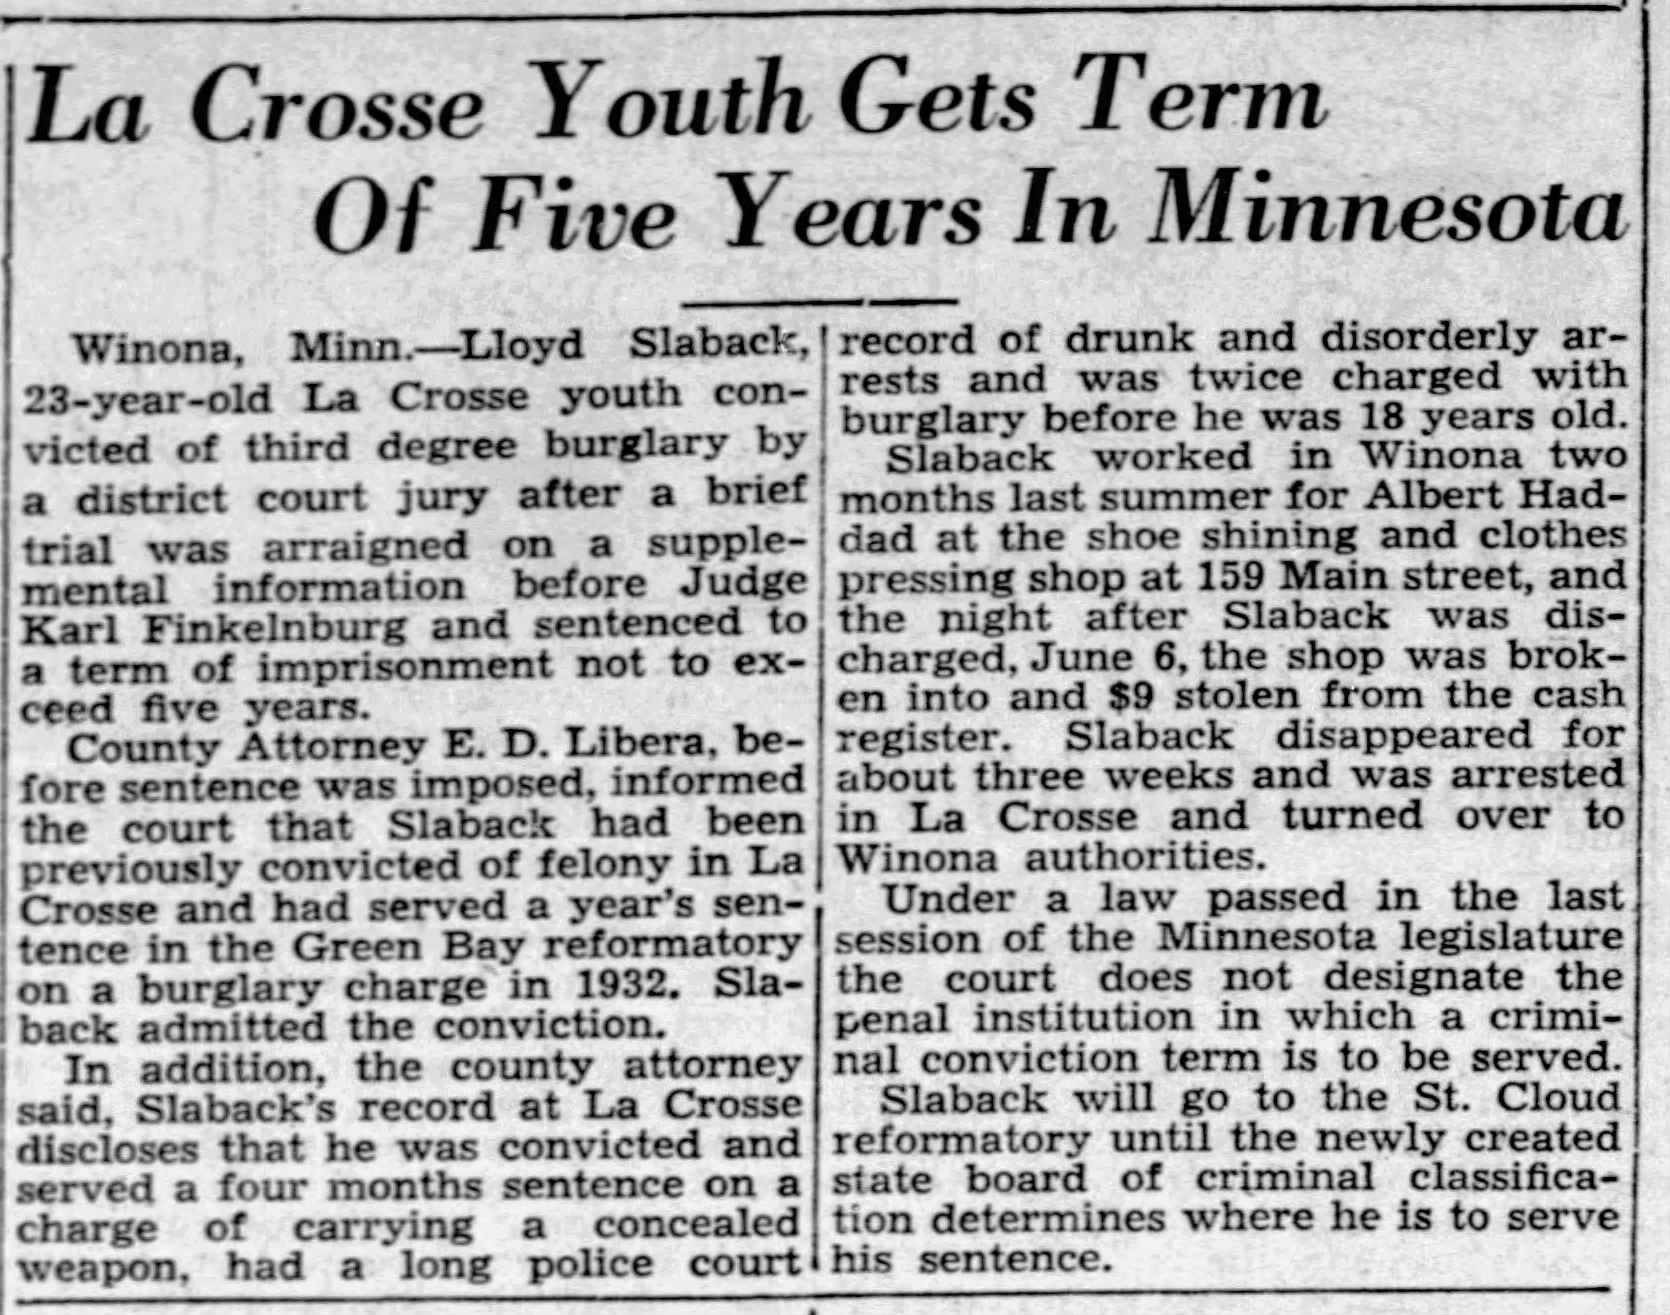
\includegraphics[keepaspectratio]{images/Akou08.jpg}}

}

\caption{Page eight of the \emph{La Crosse Tribune}, October 4, 1935}

\end{figure}%

For a few months, Lloyd had drifted around to various relatives
including his much older sister Ruby, who was living in Winona. Although
her husband, Ben, was reluctant to let him stay with them, Ruby
convinced him that it was their duty as good Christians. Lloyd was
grateful and even found a job. It looked like he might turn his life
around, but then he was arrested again. By the time of the trial, the La
Crosse newspapers had picked up the news of his latest crime.

Lila knew that Lloyd was a terrible influence, but he was also funny and
smart. Five years was an awfully long sentence for stealing nine
dollars. Aunt Hattie spent more than that just buying dresses and shoes
for the baptism.

\section{Notes}\label{notes-16}

In this chapter, Lila is getting conflicting messages. She understands
the value of giving and receiving charity, but her family is punishing
Lloyd and turning him away. Although his older sister took him in (as a
good Christian), it wasn't enough; he committed another crime and was
sent away to prison for five years.

Through \href{https://www.ancestry.com/}{Ancestry.com}, I connected with
the granddaughter of Lloyd's niece---the one who Aunt Hattie was so keen
to protect. Lloyd and his niece secretly developed a friendship and
wrote to one another for years while he was in prison. Like Lila, she
may have felt that Lloyd had been judged unfairly. In his letters, he
expressed regret for his crimes and wasted life.

This chapter raises questions about Lila's future. She is funny and
caring, but is that enough? What will be her path in society?

For more information, see Mary Bosworth, ed.\footnote{\citeproc{ref-bosworth2005a}{\emph{Encyclopedia
  of Prisons \& Correctional Facilities} (Thousand Oaks, California:
  SAGE Publications, 2005)}.}, Lawrence J. Friedman and Mark D.
McGarvie, eds.\footnote{\citeproc{ref-friedman2003a}{\emph{Charity,
  Philanthropy, and Civility in American History} (Cambridge University
  Press, 2003)}.}, and Ted Gup\footnote{\citeproc{ref-gup2010a}{\emph{A
  Secret Gift: How One Man's Kindness---and a Trove of
  Letters---Revealed the Hidden History of the Great Depression} (New
  York: Penguin Publishing, 2010)}.}.

\bookmarksetup{startatroot}

\chapter{Chapter Sixteen}\label{chapter-sixteen}

That year Theron's twin daughters, Arlene and Evelyn, were born. It was
a shock adding two babies to the family at the same time, especially
with the ongoing Depression. Theron was lucky to be employed, but money
was tight. To stretch their budget, he started doing some
semi-professional wrestling. Matches were held at the Avalon Ballroom,
close to where Uncle Frank and Aunt Hattie lived on Copeland Avenue.
Lila was never allowed to go (it wasn't a place for young ladies), but
she heard about it from Lyle and Cecil. The large ballroom had tiny
lights in the ceiling, making it look like a sky filled with twinkling
stars. Although Theron rarely won---Lyle complained that the matches
were ``fixed''---he was strong and fast enough to be a solid competitor.
He wrestled until 1937 when the Avalon closed due to a fire.

Those years were mostly a blur to Lila: endless days of cooking and
dishes and laundry and going to school. But they were also marked by a
string of tragedies. In 1936, Theron and Borgny had another daughter,
Norma Jean. It should have been a happy event, but their father was
still barely working, and their mother had become a recluse. Veda was
constantly worried about the family's finances. To earn cash, she
started taking small jobs outside of the house, such as helping an
elderly neighbor with the laundry or watching the neighbor's children
after school. Lila had to pick up the slack on the household chores, but
she didn't mind. Someone had to pay the taxes and utilities. When she
was sixteen, Theron taught Veda how to drive. They didn't have another
car, but sometimes the neighbors would hire her to run errands with
theirs---for example, to drop them off downtown and pick them up after a
day of shopping. It was easy work, but the good fortune didn't last very
long.

One day, Veda was driving Mr.~McCune and four of his grandchildren
downtown for a performance at the Rivoli Theater, when another car sped
through the intersection and crashed into them. The oldest grandchild,
Lois, was thrown out of the car, fracturing her arm and skull. They were
all badly bruised and shaken. Veda refused to go to the hospital and
started walking home; by the time she walked through the door, she was
sobbing. Although the accident was not her fault, it brought back
terrible memories of the day Earl was killed. Veda stopped driving; in
fact, she never drove again. Later in life, she would claim that she
never knew how.

Lyle also had an accident. One Saturday he borrowed the truck from
Theron and was on his way to pick up a date so they could go to the
movie theater. Just two blocks from home, an elderly man stumbled into
the road and Lyle was unable to avoid hitting him. The newspaper noted
that the man had died as police were lifting him into the ambulance.

\begin{figure}[H]

{\centering 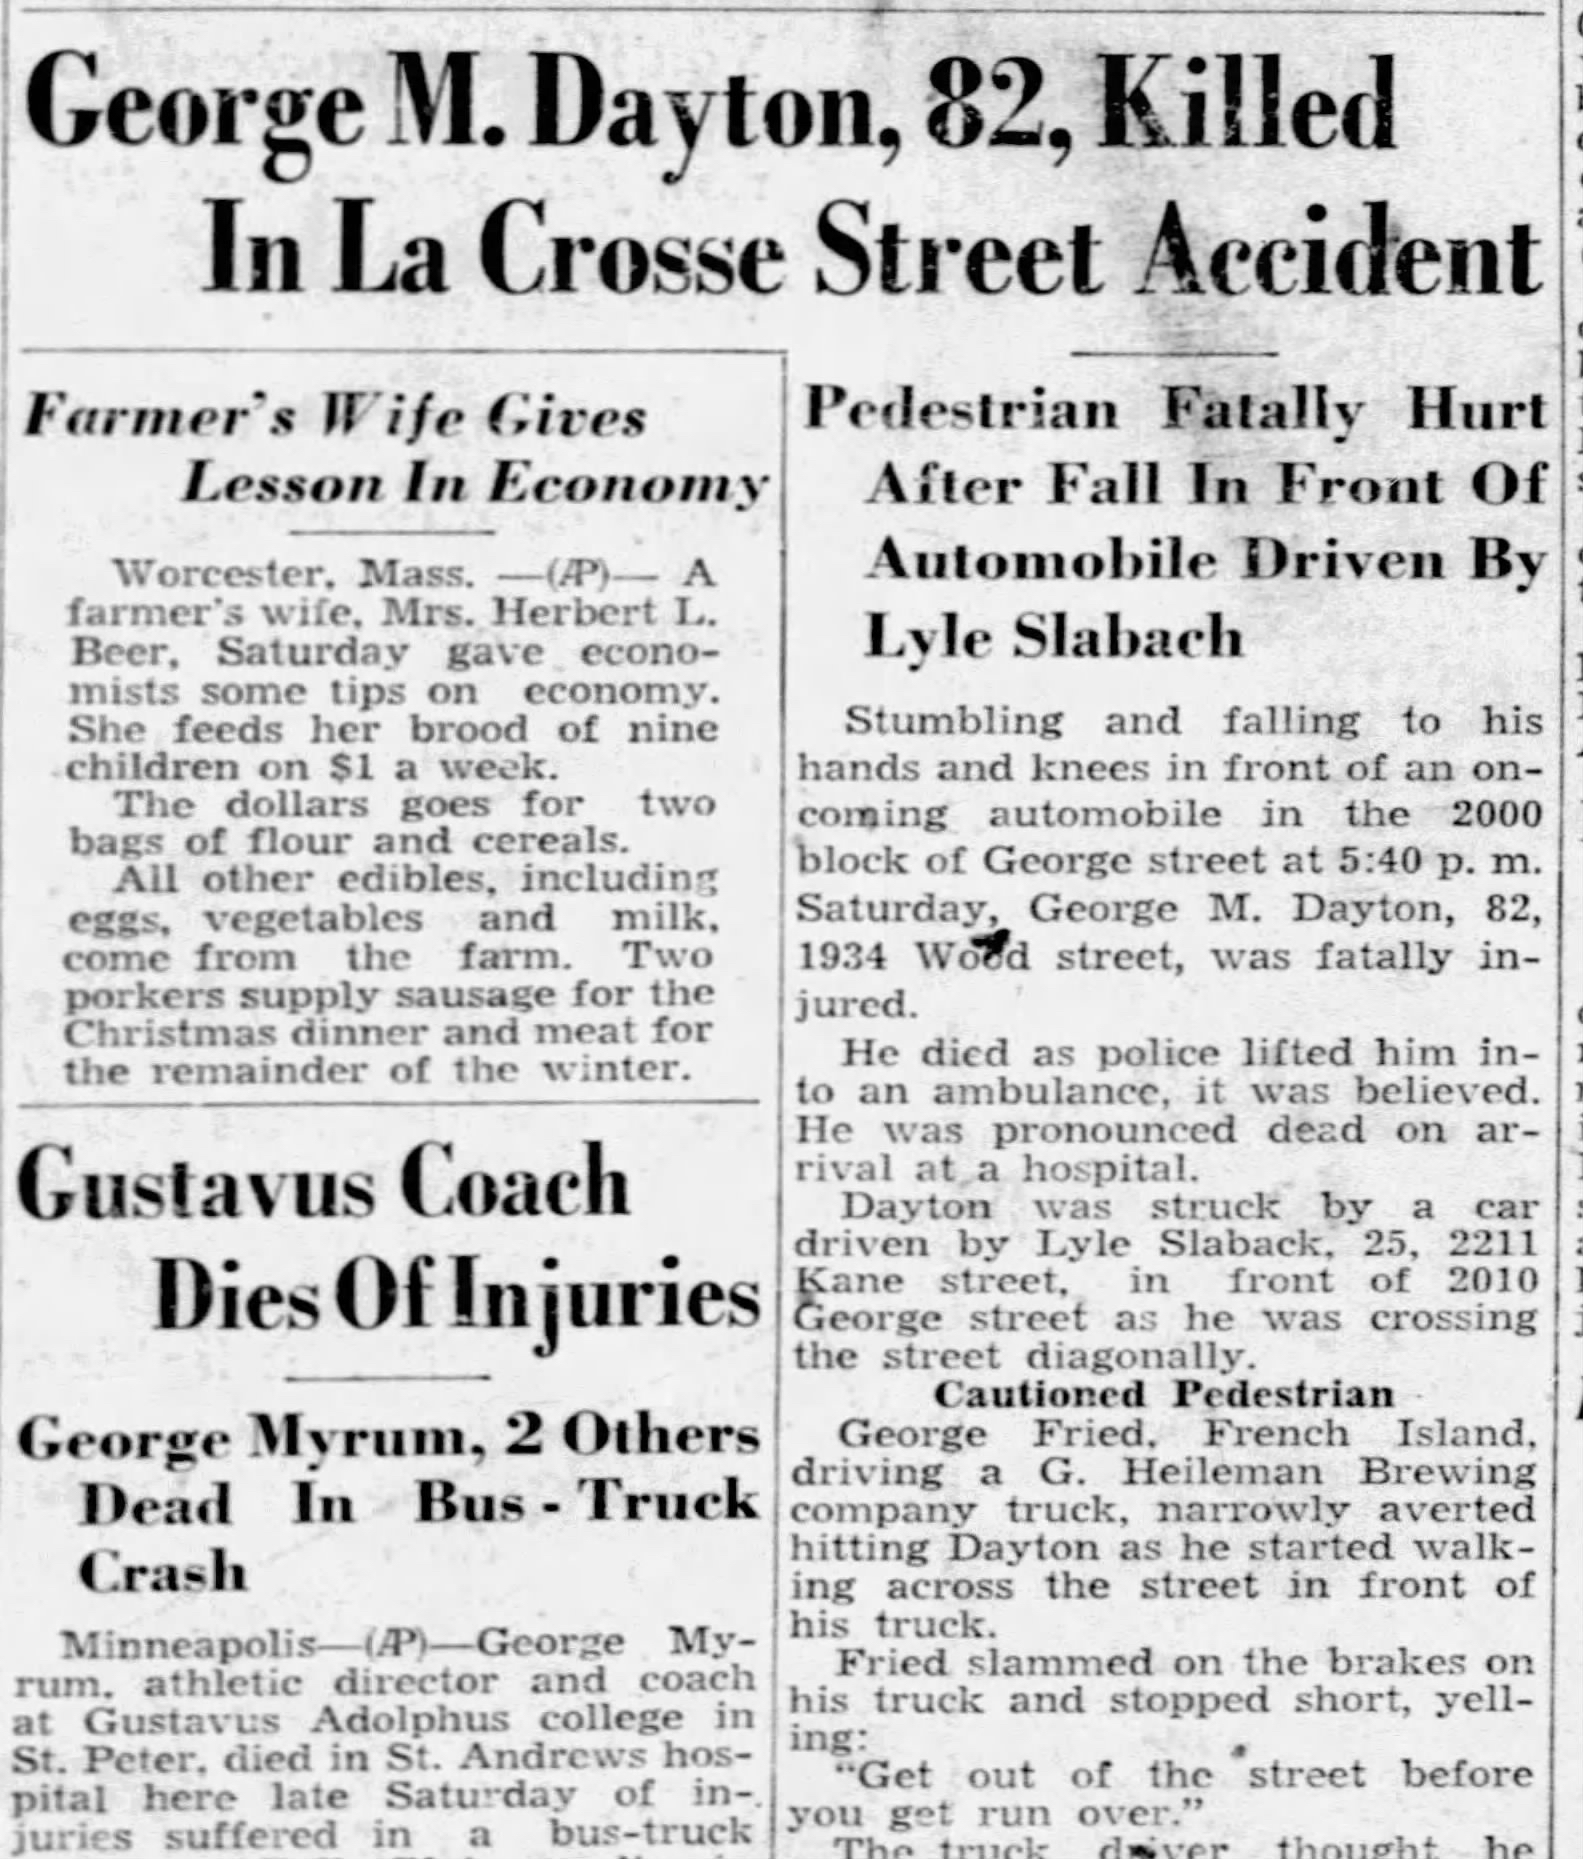
\includegraphics[width=0.8\linewidth,height=\textheight,keepaspectratio]{images/Akou09.jpg}

}

\caption{Front page of the \emph{La Crosse Tribune}, November 13, 1938}

\end{figure}%

To her parents, the accidents were further proof that moving to La
Crosse had been the wrong decision. Lila did not agree, but she was
starting to wonder if the Slaback family was cursed. One day while she
and Veda were in the basement doing laundry, she mentioned her theory.
Veda's eyes opened wide, and she said, ``Do you really think so?'' Veda
shuddered and added, ``Let's try not to think about it. There's nothing
we can do whether it's true or not.''

That was also the year that Cecil became a father. The girl's father was
furious that his sixteen-year-old daughter was pregnant. They had a
``shotgun wedding,'' and Gladys had to drop out of school to have the
baby. It was an event that filled Lila with both horror and interest;
she was struggling in school and often wished that she could drop out.

\section{Notes}\label{notes-17}

Since Theron was so much older than Lila, I didn't know anything about
him when I started writing this book. I learned about his brief career
as a semi-professional wrestler by reading archival newspapers. Boxing
and wrestling were popular entertainments in the 1920s and 1930s.

I learned about the car accidents from newspapers and did the math on
Cecil and Gladys. These were not fun, family stories the Slabacks wanted
to hand down to the next generation (like me); they were shameful
secrets that nobody wanted to talk about. In this chapter, Lila is in
her early teens. In her family's silence, she is forming her own ideas
about how the world works.

For more information, see Scott Beekman\footnote{\citeproc{ref-beekman2006a}{\emph{Ringside:
  A History of Professional Wrestling in America} (London: Bloomsbury,
  2006)}.}, Jeffrey Sussman\footnote{\citeproc{ref-sussman2019a}{\emph{Boxing
  and the Mob: The Notorious History of the Sweet Science} (Lanham,
  Maryland: Rowman, 2019)}.}, and Nicholas L. Syrett\footnote{\citeproc{ref-syrett2016a}{\emph{American
  Child Bride: A History of Minors and Marriage in the United States}
  (Chapel Hill: University of North Carolina Press, 2016)}.}.

\bookmarksetup{startatroot}

\chapter{Chapter Seventeen}\label{chapter-seventeen}

Hazel seemed to have given up on life. During the day, she stayed in her
bedroom and slept. At night, she listened to the radio and drank
whiskey. Lyle was the one who bought it for her. Nobody talked about
Hazel's drinking problem, but Lila knew; she had never been a good
sleeper and often saw her sitting alone late at night. On the rare
occasions when Hazel ventured outside, the neighbors would always say,
``Why hello, Mrs.~Slaback, I haven't seen you in ages! Good to see you
up and about,'' but Lila was sure they could see that something was very
wrong. Hazel was gaunt and her hair had turned completely gray.

Aunt Hattie was the one who decided that something must be done. Lila
was wary about her schemes, but on this she had to agree: her mother's
behavior was not normal. The cure, Aunt Hattie said, was to get Hazel
back into the community; being of service to others would help her stop
focusing so much on her own situation. When presented with the idea,
Hazel said, ``Fine, but no churches; I will never stop being angry at
God for taking my son away.'' Lila's heart skipped a beat; it was the
first time her mother had said anything about the cause of her turmoil.
Without batting an eye, Aunt Hattie said that would be no problem; the
American Legion Auxiliary and Wilson Colwell Relief Corps were always
looking for new members.

Much to Lila's surprise, within a few months her mother was an officer
for three different organizations. Hazel's specialty was running
``bunco'' games for charity. Everyone knew that bunco was a dice game of
pure luck---associated with speakeasies and criminals---but it gave
Hazel a dark sense of glamour. It also raised a lot of money. Hazel
started joining the family for meals and regained the weight she had
lost, but she never stopped drinking entirely. Later in life, she took
up rug braiding as a hobby, keeping a stash of whiskey in her box of
fabric strips.

\begin{figure}[H]

{\centering 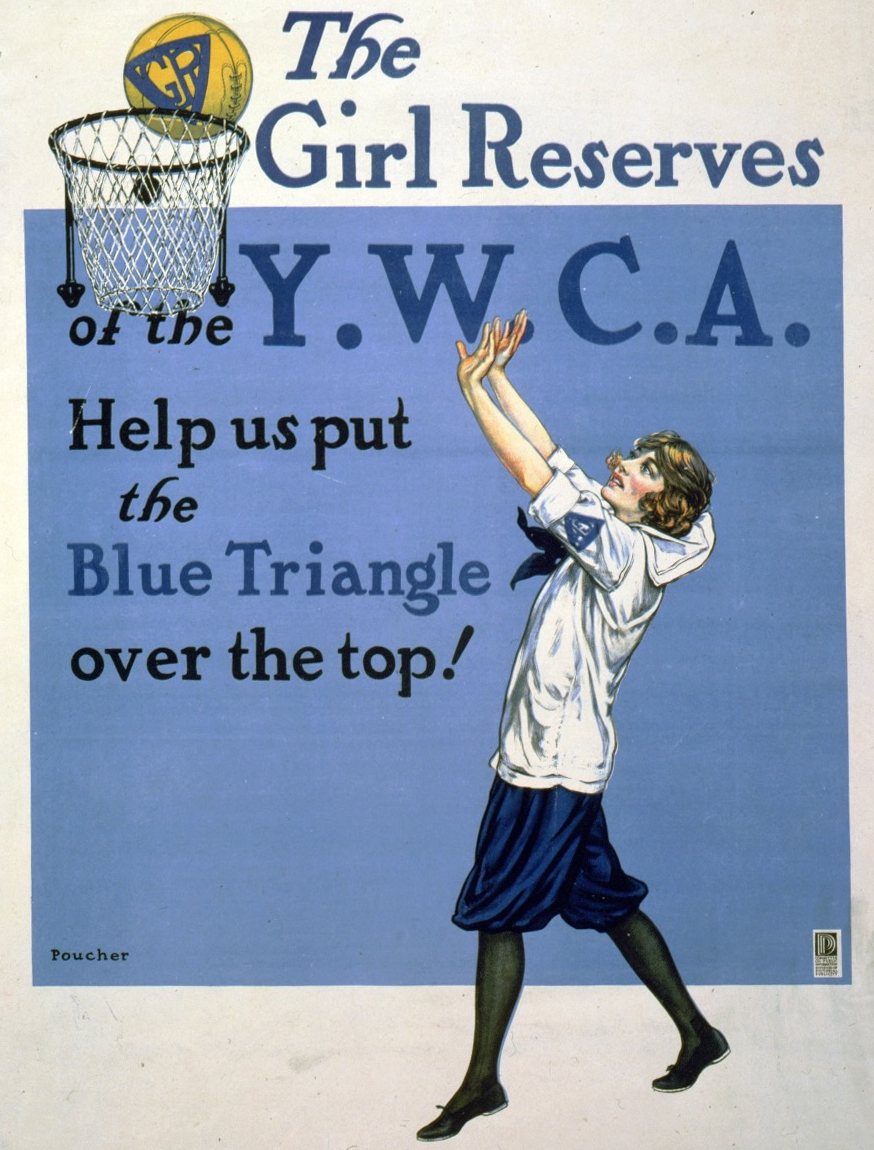
\includegraphics[width=0.75\linewidth,height=\textheight,keepaspectratio]{images/Akou10recropped.jpg}

}

\caption[Poster advertising the YWCA and Girl Reserves]{Poster
advertising the YWCA and Girl Reserves; Library of Congress Prints and
Photographs Division, \# LC-USZC4-5551}

\end{figure}%

Lila joined the Girl Reserves. Ironically, Aunt Hattie had switched from
being concerned that Lila would never get invited to parties to being
worried that she was a ``fast'' girl who would bring shame to the
family. Her daughter, Opal, had been in the Girl Reserves, and she
thought it was outstanding for building good character.

Lila knew the group required uniforms and was worried about the cost,
but Aunt Hattie assured her that she would pay for it. Lila was excited
for an opportunity to get out of the house and to do something on her
own. Aunt Hattie still had her daughter's old uniform; unfortunately, it
was too small for Lila to wear. Lila was relieved when she hired a
dressmaker to make a new one instead of taking her shopping. The outfit
had a white shirt, blue culottes (which felt odd, since Lila had never
worn pants for anything besides chores), and a blue kerchief. It made
Lila feel like she was posing for a box of Cracker Jacks. During the
fitting, the dressmaker asked her why she kept giggling. Lila stopped
and made up a lie to avoid seeming rude, ``Oh\ldots I was just thinking
about something I heard at school today.'' The dressmaker's daughter had
also been in the Girl Reserves; she told Lila how proud she was of her
daughter, who was all grown up and married with children of her own.

At the first meeting, Lila received a small poster with the group's
pledge that she could hang in her bedroom. She had to admire how the
first letter of each line spelled out the name of the organization. It
would make the pledge easier to memorize.

\begin{quote}
``\textbf{As a Girl Reserve, I will try to be}''

\textbf{G}racious in manner\\
\textbf{I}mpartial in judgment\\
\textbf{R}eady for service\\
\textbf{L}oyal to friends

\textbf{R}eaching toward the best\\
\textbf{E}arnest in purpose\\
\textbf{S}eeing the beautiful\\
\textbf{E}ager for knowledge\\
\textbf{R}everent to God\\
\textbf{V}ictorious over self\\
\textbf{E}ver dependable\\
\textbf{S}incere at all times
\end{quote}

She was skeptical about her ability to live up to it. ``Maybe Veda could
do it,'' she thought to herself. Veda never complained about the chores.
She was beautiful, hard-working, loyal to her friends, practically
perfect in every way. Lila admired and loved her, but at times she
wanted to hammer a nail into her perfect forehead.

Nothing she did would ever be as good as Veda. Veda was a ``good girl.''
Earl had also been a ``good boy.'' He could never be bad, since being
dead prevented him from doing anything wrong. Lila reflected that the
rest of them took turns being the ``bad one.'' Theron had killed Earl.
Lyle killed that pedestrian. Cecil had a shotgun wedding. All of those
things were pretty bad. Lila had never done anything like that, but she
was not a young lady like Veda. She ate too much, laughed too much, and
asked too many questions. She hated doing the chores and had to be
reminded sometimes to do them. She wasn't a good student or as popular
as Veda. She wasn't sure it was possible (or even desirable) to be one
of the good ones.

\section{Notes}\label{notes-18}

Life has taught me that when times are tough, people notice. They might
not say anything, but they see what is happening. Our bodies reflect our
inner turmoil.

My mother told me that her grandmother (Hazel) always kept a bottle of
whiskey in her box of supplies for making braided rugs. Multiple people
have told me that she was not an easy person to get along with. In an
earlier version of this book, I described Hazel's life as a child and
young woman, trying to make sense of how she turned into a bitter adult
with a drinking habit.

In the late 1930s, Hazel Slaback suddenly began to appear in the
newspapers; this was normal for Aunt Hattie and Borgny (Theron's wife),
but not for her. I suspect that Aunt Hattie nudged her to get involved
in charity work, but it was always for secular organizations. Lila was
listed in the newspaper as a member (and once as an officer) for the
Girl Reserves, an organization for white, adolescent girls to develop
``good character,'' similar to the YWCA or Camp Fire Girls. In this
chapter, we get insight that Lila knows what her family and society
expect her to do, but she is not sure that she is capable of doing it
(or even wants to). This is a hint that her life might take a more
scandalous turn.

In the 1930s and 1940s, ready-to-wear was not as common for women as it
was for men. It would not have been unusual to hire a dressmaker or to
make an outfit at home.

For more information, see Jennifer Helgren\footnote{\citeproc{ref-helgren2022a}{\emph{The
  Camp Fire Girls: Gender, Race, and American Girlhood, 1910--1980}
  (Lincoln: University of Nebraska Press, 2022)}.}, Jenna Weissman
Joselit\footnote{\citeproc{ref-joselit2014a}{\emph{A Perfect Fit:
  Clothes, Character, and the Promise of America} (New York: Henry Holt;
  Company, 2014)}.}, and Nina Mjagkij and Margaret Spratt,
eds.\footnote{\citeproc{ref-mjagkij1997a}{\emph{Men and Women Adrift:
  The YMCA and the YWCA in the City} (New York University Press, 1997)}.}

\bookmarksetup{startatroot}

\chapter{Chapter Eighteen}\label{chapter-eighteen}

Life was a bit easier when their father started working again. With
Cecil out of the house, there was also one less mouth to feed. Veda
continued doing odd jobs, but now she was allowed to keep and use some
of the money. One weekend she suggested to Lila that they should take a
walk. Lila protested, ``Really? I'm so tired\ldots I don't want to go
anywhere,'' but Veda insisted. It was a hot, muggy evening. As they
walked along the river, Lila complained about the swarms of gnats and
mosquitoes; she was going to be covered with bites. Veda said, ``Better
keep walking then\ldots it won't be much farther.'' Lila was just about
to insist that it was time to turn back when they suddenly reached their
destination: the Riviera Theater, which was showing \emph{The Wizard of
Oz}. ``Surprise!'' said Veda. Lila could not believe it. Were they
really going in? She had heard about the movies, but she had never seen
one. She must have had a real look of surprise on her face because Veda
squealed and gave her a big hug.

It was forty cents for two tickets plus popcorn. There were four ushers
wearing uniforms; red suits trimmed with gold braid and shiny black
shoes. One of them took their tickets and led them to seats in the
middle of the theater. There was a stage in front with a large velvet
curtain. Lila started to eat her popcorn while they were waiting; it was
so salty and delicious. It was not Veda's first movie---earlier in the
year, she and her friend Rebecca had seen \emph{It's a Wonderful
World}---but they were both very excited. As the lights dimmed and the
curtain lifted, Lila felt like she was being transported to another
world. It was an incredible sensation, soon enhanced by Dorothy's own
journey to the land of Oz. The colors were like jewels. Who wouldn't
want a pair of ruby slippers or a magic wand or to have such wonderful
friends? By the time Judy Garland sang, ``Somewhere Over the Rainbow,''
Lila was completely transfixed.

They talked about the film all the way home and for days afterward. Lila
said that her favorite part was when the Tinman, the lion, and the
scarecrow snuck into the castle and melted the witch with a bucket of
water. To Veda's horror and secret delight, Lila imitated the speech for
days, especially when they were washing the dishes. ``I'm
melting\ldots melting! Ohhhhh what a world, what a world.'' Veda said
her favorite was when they arrived at Oz, and they all went to the
beauty parlor for some washing and polishing. Wasn't Dorothy just
breathtaking? Lila had to admit that she was, but it made her feel a bit
sad. She would never be as beautiful as Dorothy or have such a grand
adventure. There was no yellow brick road in La Crosse.

\begin{figure}[H]

{\centering 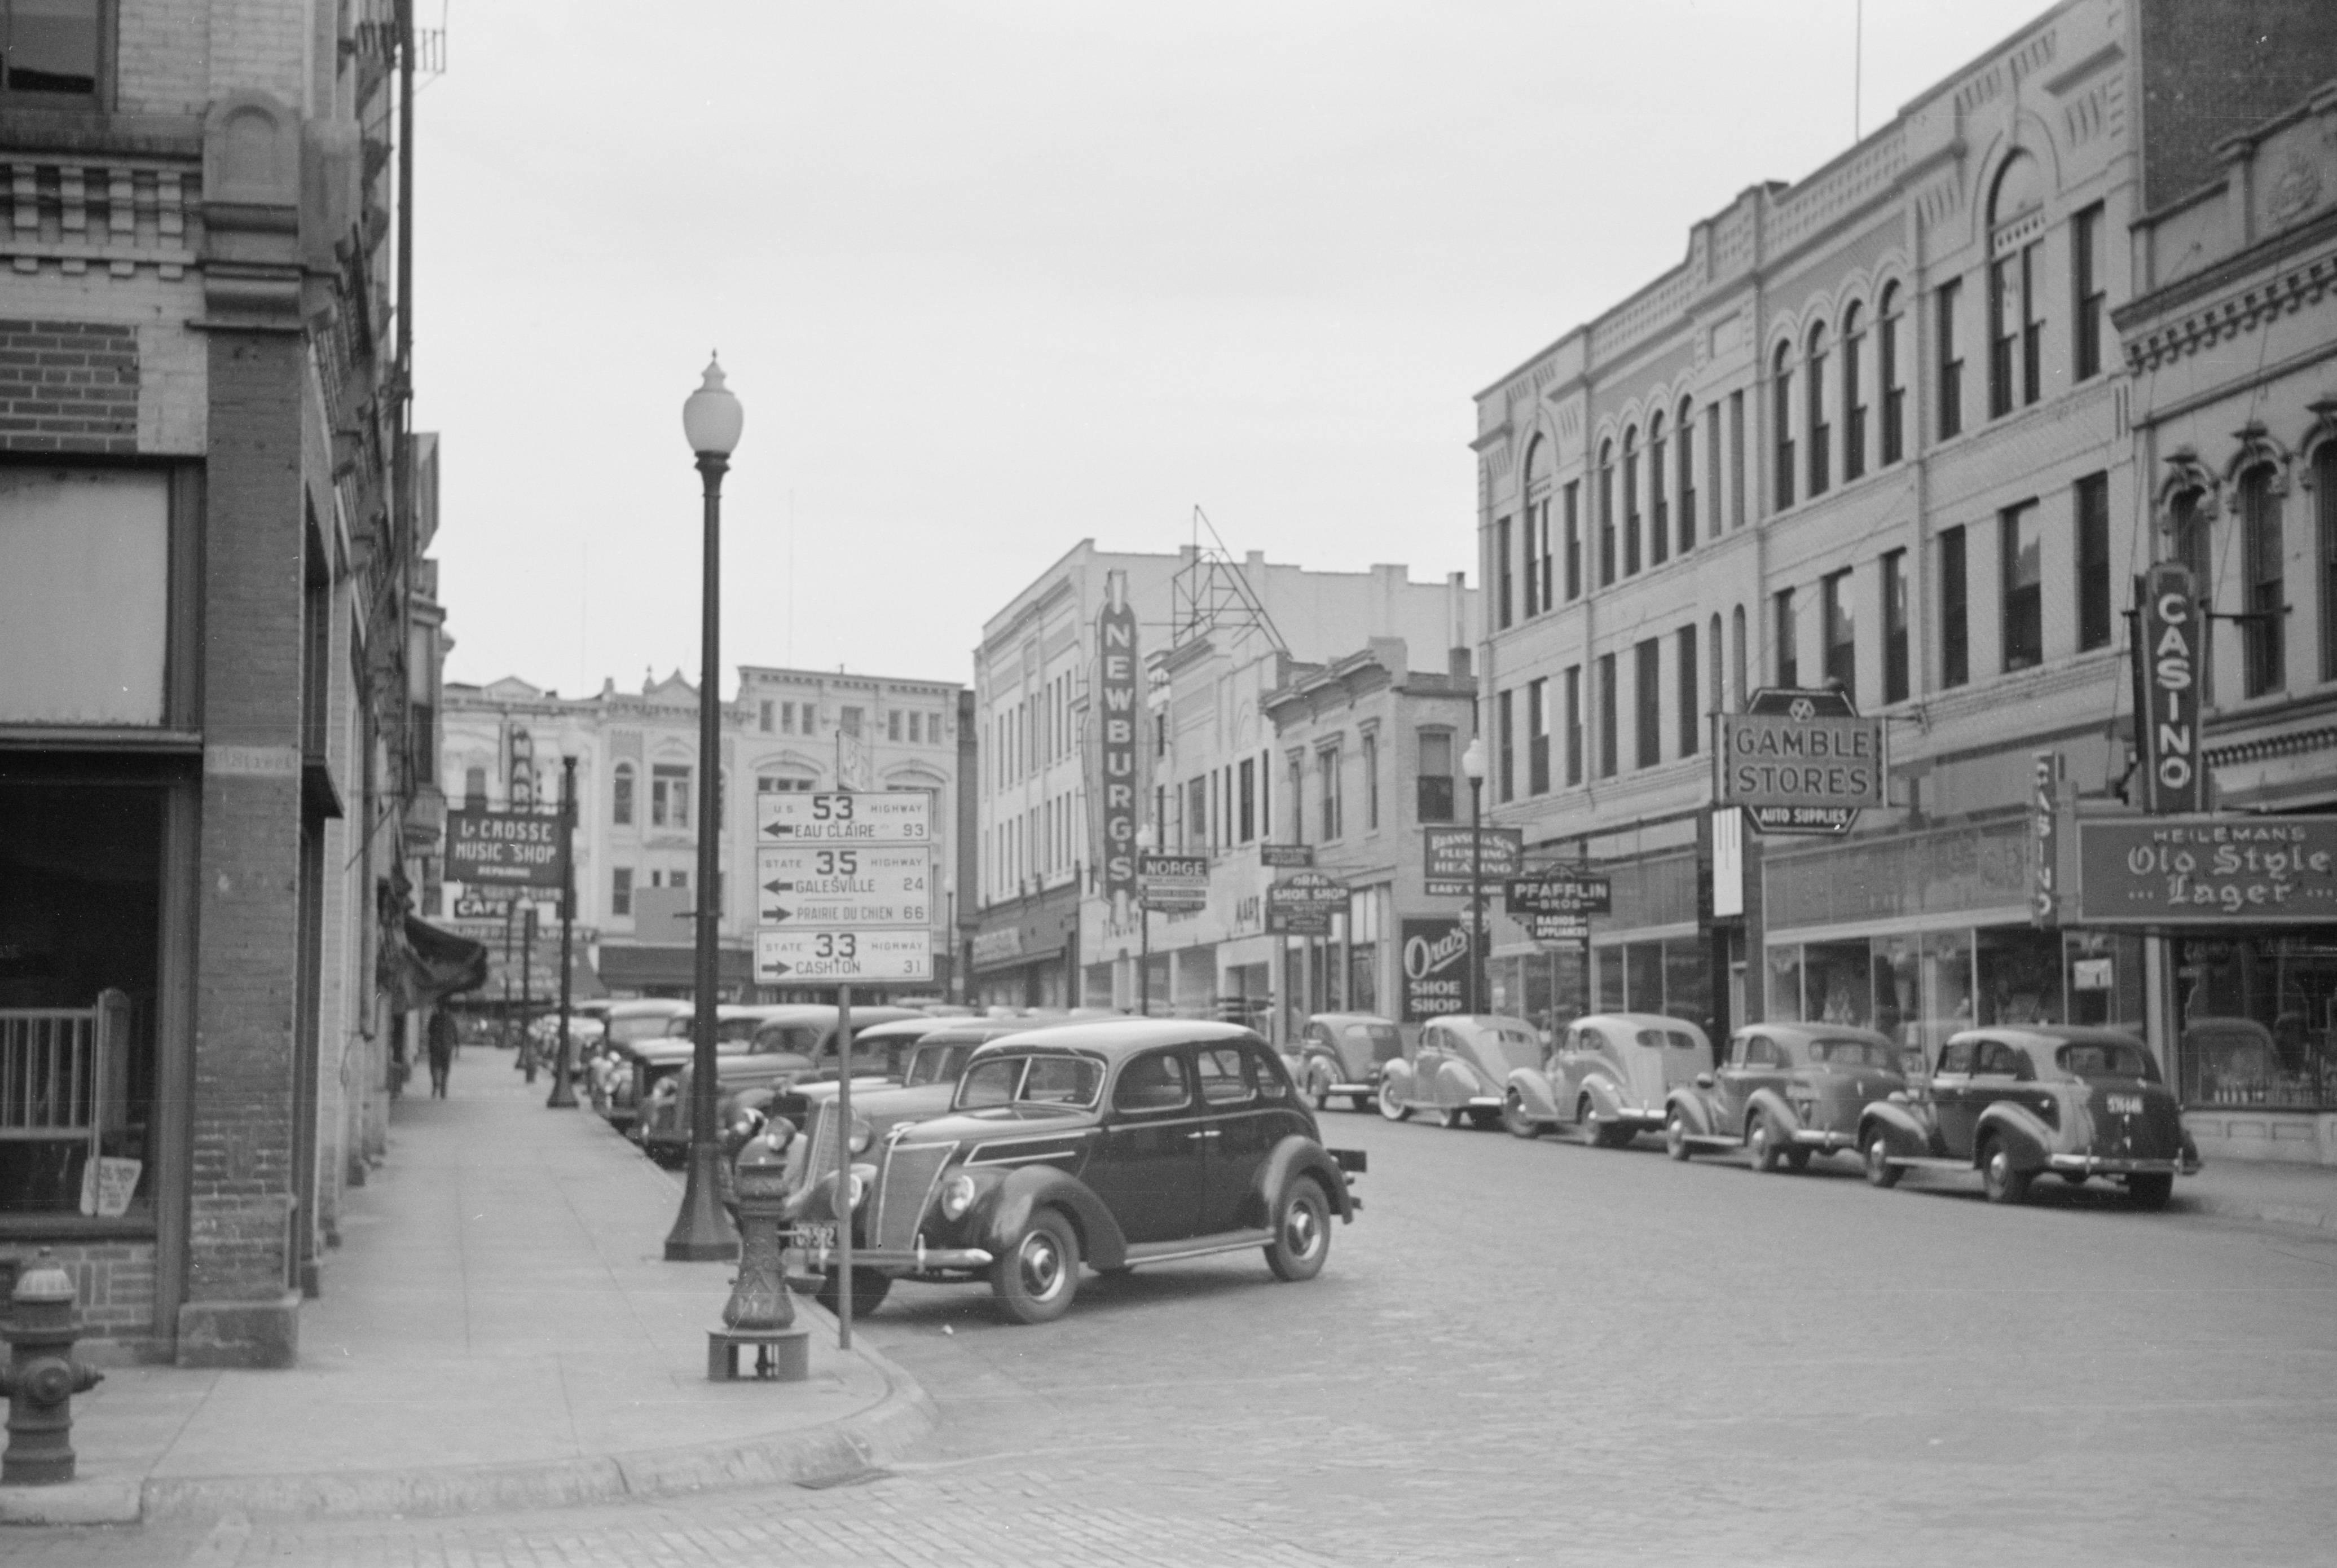
\includegraphics[width=1\linewidth,height=\textheight,keepaspectratio]{images/Akou11.jpeg}

}

\caption[A busy street in downtown La Crosse, 1939]{A busy street in
downtown La Crosse, 1939; Library of Congress Prints and Photographs
Division, \#LC-USF33-003068-M2}

\end{figure}%

Lyle often took his dates to the movies. Since Veda and Lila were not
dating yet, they decided it was best to go with one another; it was not
too difficult to earn forty cents, especially now that Lila was also
taking odd jobs. Her specialty was childminding. Some mothers in their
neighborhood (like Borgny, for example) stayed at home---especially if
they had many children or their children were not yet old enough for
school---but there were plenty who worked outside of the home, mostly in
factories. Hiring a young woman to mind the children between the end of
the school day and the end of the workday was an affordable way to make
sure they were fed and kept out of trouble. Hazel gave them a stern
warning that their ``adventures'' better not interfere with the cooking
and cleaning, but in the end, it made no real difference. Veda and Lila
just did the chores more efficiently.

A few months later they saw \emph{Gone with the Wind}. For different
reasons, they were both captivated by Scarlett O'Hara. Veda wanted her
clothing; she was obsessed with the bounce of her hoopskirts, the
elegant fabrics, and her coquettish way of wearing hats. Veda said it
was an ``inspiration.'' Lila wanted to \emph{be} Scarlett. She was
beautiful, but she was also a firecracker. She wasn't afraid to break
the rules; she knew what she wanted, and nobody was going to stop her.
For two young women quickly approaching the age of marriage, the movie
made a serious and lasting impression. It was not just entertainment.
Veda wanted to be like Scarlett's friend and sister-in-law, Melanie
Hamilton Wilkes; she proclaimed how romantic it would be to marry a
soldier going off to war. Lila thought Scarlett's relationship with
Rhett Butler was much more passionate and exciting. It was the first
movie they went to see twice.

\section{Notes}\label{notes-19}

1939 was a landmark year in Hollywood. \emph{Gone With the Wind} and
\emph{The Wizard of Oz} were two of the year's blockbuster films. Based
on popular books and produced in full color, they captivated audiences
and are still popular in the United States today. Both featured young
heroines close in age to Lila (who turned seventeen that year); if she
had seen one or both films, I imagine they would have made quite an
impression. Archival newspapers helped me determine which theaters in La
Crosse were showing those films. My father (born in 1945 in a smaller
town in Wisconsin) told me often as a child how it only cost him
twenty-two cents to see a movie and buy popcorn.

This chapter reminds us of Lila's sense of humor. It also explores the
differences between Lila and her sister Veda. They are living in the
same family and seeing the same films but getting wildly different
insights from them. The movies were teaching them about friendships and
romantic relationships in a way that was very different from previous
generations. To their parents, the movies probably seemed like ``just an
entertainment'' or even a waste of time and money. My description of the
theater attendants draws from my own research on historic work uniforms
using photographs and trade catalogs from uniform manufacturers.

Childminding seems to have been a common occupation for older girls and
young women in La Crosse in the 1930s and 1940s. The newspaper was full
of short advertisements for ``girl wanted'' as a childminder or
part-time housekeeper. The 1940 Census and telephone records reinforce
just how many adult women in La Crosse were working outside of the home.

For more information, see Akou\footnote{\citeproc{ref-akou2024a}{\emph{On
  the Job}}.}, Ina Rae Hark, ed.\footnote{\citeproc{ref-hark2007a}{\emph{American
  Cinema of the 1930s: Themes and Variations} (New Brunswick, New
  Jersey: Rutgers University Press, 2007)}.}, and Robert B.
Ray\footnote{\citeproc{ref-ray2020a}{\emph{A Certain Tendency of the
  Hollywood Cinema, 1930--1980} (Princeton University Press, 2020)}.}.

\bookmarksetup{startatroot}

\chapter{Chapter Nineteen}\label{chapter-nineteen}

When Veda and Lila went back to school in January, Viola Johnson
announced that she was dropping out of school to get married. It was not
the first time this had happened; the first was Lila's friend, Kathleen,
who got pregnant when she was fifteen. Her boyfriend, Michael, was only
sixteen, but their parents---who were all Catholic---insisted that they
fix the problem immediately by getting married. Lila had attended her
wedding. As she had always dreamed, the wedding was big and so was her
dress. Despite being ``knocked up,'' it was a beautiful day. The church
was packed, and Kathleen was radiant. Two years later, with two children
and a third on the way, she still claimed that she was thrilled with her
new life. Lila wondered if that was really true; her own mother was
never thrilled by anything. Kathleen and Michael were living with his
parents until they could save enough money for a house of their own.

Unlike Kathleen, who was nearly the same age as her husband, Viola's
husband-to-be, John Schneider, was several years older. How did they
meet? Viola wouldn't say. Everyone knew that her first love was Samuel
Collins, but her father wouldn't give Viola permission to marry (or even
date) one of those dirty Irish Catholics. Later, Lila heard that Viola's
father had discovered that Viola and Samuel were holding hands and
passing love notes in school. His solution was to find her a good
Lutheran man and get her married as quickly as possible. The fact that
she was months away from getting her high school diploma made no
difference. Even Viola's mother agreed that it was a waste of time for a
woman to plan a career; Viola should be planning to have children and
then stay home to raise them. Viola was a good student, but she was also
a good girl. She knew it was no use arguing with her parents. A few
months later, her sister Myrtle also decided to drop out of school and
marry John's younger brother, Carl. Myrtle had never dated and was giddy
to be a ``real woman.''

Like Viola, Veda was also a good student. She had her eyes set on
finishing her degree and becoming a nurse, not on dating. As a result,
she was the first member of the Slaback family to graduate from high
school. Lila thought her parents should have been proud; curiously, they
were indifferent. As long as Veda continued to do her chores, it didn't
seem to matter what she did with the rest of her time. They never said
that school was a waste of time for a woman, but they also never
encouraged her to pursue anything besides getting married. (To be fair,
they also never encouraged the boys to finish school or to get a job
outside of the family business.) Veda reasoned that she would need to
work for at least one year to earn enough money for nursing school, so
she applied to work as an usher at the Riviera. Lila thought it was a
brilliant move. She could earn money and watch the movies for free.

That job was where Veda met Red. He was two years older than Veda and
was living at his uncle's house until he could afford to move out. At
the end of her first shift, Red offered to walk her home. ``You never
know what kind of hooligans might be roaming at night, waiting to take
advantage of a beautiful young woman like yourself.'' Veda blushed and
accepted his offer. Although his real name was Francis, everyone called
him ``Red'' because of his hair. His parents were Catholic and had ten
children. Red was the oldest one; he had moved to La Crosse to find
work. Veda couldn't stop talking about him. Red is so handsome! Red has
such a funny laugh! Did I tell you what he said about that new Disney
film, Pinocchio?

One day Lila stopped her in midsentence and said, ``Veda, I'm tired of
hearing about Red all the time. Are you in love with him or something?''

Veda's mouth dropped open, and she said, ``Yes, I suppose I am.''

They decided to invite him for dinner. Veda said she was nervous, but
they agreed that there was no point in trying to keep a relationship
secret; someone in the family was bound to find out eventually. Why not
just get it out in the open? It was January, so they decided to have him
over on Sunday and make a big, hearty pot of beef stew. Veda said she
heard that ``the way to a man's heart is through his stomach.'' It might
not be true, but why take chances? Although they didn't tell anyone that
Red was coming over for dinner, the whole family was there, even Cecil
and Gladys and their daughter, Deanna (who Lila's mother said was
``totally spoiled''). He rang the doorbell promptly at 6:00 and Lila
answered the door. She had imagined that he would be tall and handsome,
but aside from having red hair and freckles, he was actually pretty
average. Lila wondered what Veda saw in him. Red politely asked, ``Is
Veda home?'' and Lila stood aside with a sweep of her arm, indicating
that he should enter.

Dinner was oddly quiet. Lila wondered if Red was going to ask for Veda's
hand, but it seemed that he was truly just there for dinner. As usual,
her father and brothers talked business. One of their neighbors was
moving to Iowa to be with her daughter (who had five children and
another one on the way); she had hired them to fix all the woodwork and
refresh the plaster. It was an old house, so there was plenty of work to
do. Finally, her father said, ``So\ldots Red, is it? Tell us a little
about yourself.''

He went back to eating his stew, and Red stammered, ``Well, I guess
there isn't too much to say. My parents are farmers; they live in
Marquette County, about halfway between La Crosse and Sheboygan. I came
to La Crosse to look for a different line of work\ldots I supposed I'm
not too interested in being a farmer.'' John's father nodded his head;
it was the same choice he had made years earlier.

Lila's mother spoke up and said, ``Do you have any brothers or
sisters?''

``Yes ma'am, four brothers and five sisters. I'm the oldest.''

Veda (who was usually silent at dinner) spoke up and said, ``We work
together at the Riviera Theater.''

And surprisingly, that was it. As soon as Veda spoke, the conversation
moved on. They had chocolate cake and coffee for dessert. Red said that
he ``better get going'' and Veda walked him to the front door. Did
anyone notice that Veda was in love?

When they cleared and washed the dishes, Lila noticed that Veda had
regained some of the color in her face. Veda said, ``Well that went
alright.''

Lila said, ``Yeah, I guess. What are you going to do now?''

Veda said, ``I don't know. Keep working together, keep walking home
together\ldots watch movies.'' Lila thought it sounded pretty boring.
Why settle for the first man who showed an interest when you were as
beautiful as Veda? Scarlett O'Hara didn't settle for Rhett Butler just
because he wanted her to.

\section{Notes}\label{notes-20}

In the 1930s and 1940s, it was not unusual for teenagers in the Midwest
to drop out of high school, especially if they were getting married or
if the family needed them to work. Girls in particular were not strongly
encouraged to finish school. Census records tell me that Viola married
as a teenager. Her husband, John Schneider, was several years older and
had been out of school for years; it seems unlikely that they would have
met without family intervention. I have no idea if Viola had a crush on
an Irish Catholic classmate, but many Protestants in the US viewed them
with deep suspicion and would have considered such a match to be highly
inappropriate.

I learned about Francis ``Red'' Metcalf and his family mostly from the
1940 US Census. Veda and Lyle were the first members of the Slaback
family to pursue recreational dating; Veda just settled on a partner
more quickly than her older brother. Unlike John and Hazel Slaback, Red
migrated to the big city on his own before getting married.

American author and journalist Franny Fern (1811--1872) is credited with
coining the now-common advice, ``The way to a man's heart is through his
stomach.''

For more information, see Jay P. Dolan\footnote{\citeproc{ref-dolan2010a}{\emph{The
  Irish Americans: A History} (New York: Bloomsbury USA, 2010)}.},
Thomas D. Snyder\footnote{\citeproc{ref-snyder1993a}{\emph{120 Years of
  American Education: A Statistical Portrait} (Washington, DC: U.S.
  Department of Education, 1993)}.}, Syrett\footnote{\citeproc{ref-syrett2016a}{\emph{American
  Child Bride}}.}, and Joyce W. Warren\footnote{\citeproc{ref-warren1992a}{\emph{Franny
  Fern: An Independent Woman} (New Brunswick, New Jersey: Rutgers
  University Press, 1992)}.}.

\bookmarksetup{startatroot}

\chapter{Chapter Twenty}\label{chapter-twenty}

Not long after the dinner with Red, Lyle announced that he was getting
married. Lyle and Allene met through Aunt Hattie; her daughter, Ruby,
knew the bride's family from church. Since Allene's family lived in
Minnesota, the wedding would be held across the river in Winona. With
hardly a pause in the dinner conversation, their father said,
``Congratulations, Son, it's about time.'' Lyle was twenty-six and had
dated so many women; the whole family had started to wonder if he would
ever settle down. Veda said she would ask for the day off from work.

On the day of the wedding, the weather was gorgeous. It had been a cool
spring, but it was warm and sunny on that particular day in June. The
apple and plum trees were in full bloom and the farmers were busy
planting their fields. Everything smelled so fresh and green. Lila,
Veda, and Looy rode to the wedding with Cecil and Gladys; their parents
were riding with Uncle Frank and Aunt Hattie. Lila smiled all the way to
Winona, basking in the sun; it was a relief to be away from the adults.
With a little of the money she had earned by childminding, Lila had
hired one of the neighbors to make her a dress. She had slimmed down as
a teenager and loved how the light green dress fit closely around her
waist and hips. When she tried it on, the neighbor told her, ``You look
so glamorous!'' A few days before the wedding, Lila had set her hair
into a finger wave and shined her shoes. That morning, she picked a
peony bud and pinned it near her left shoulder. For the first time she
could remember, she felt truly beautiful. She wished she could wear
lipstick but knew her parents wouldn't approve. Lipstick was for whores.

Allene was six years younger than Lyle, but hardly a child bride. She
wore a dress that had been passed down through her family. It was white
with beautiful panels of handmade lace and embroidery around the bodice
and hem. She also wore a crown of flowers instead of a veil. The effect
was glorious; Lyle looked like he was ready to burst with joy and
desire. The church was full, mostly with members of the bride's family.
Lloyd was still in prison, but Lila thought of him. What was it like in
Stillwater? Lila wondered if he would return to La Crosse and if the
family would ever forgive him. She felt sorry for Lloyd. He had made
some mistakes, but the punishment had been very harsh.

When Lyle and Allene said their vows, Veda cried silently into her
handkerchief. Lila gave her a nudge to say, ``This isn't a
funeral\ldots{}'' and Veda whispered, ``I'm just so happy for them.''
When the ceremony was finished, everyone walked across the street to
another building. It was filled with tables and chairs and there was a
long table piled with food: big platters of ham and beef roast, spring
vegetables, loaves of bread, big pitchers of beer, and the largest cake
that Lila had ever seen. Lyle had just married into a family of
German-Hungarian farmers. As Lila would soon learn, there was nothing
they loved more than a beautiful wedding celebration with good food,
good beer, and good music.

The bride's father thanked everyone for coming to the wedding and wished
the couple many years of health and happiness. By the time everyone had
a plate of food, the musicians were warming up for a lively night of
dancing. Lila had a glass of beer with her lunch and was already feeling
very relaxed. One of Allene's cousins asked her to dance, and she
eagerly agreed. She had no idea what she was doing but quickly realized
that it didn't matter. The group was moving in a circle and would just
pull her back and forth; it was exhilarating. All the younger people
were dancing---even some of the older people---and the time flew by.

It was very late when they left the wedding. Cecil and Gladys were also
having a good time. It was like the wedding they wanted but didn't get
to have. When Lila's parents left that afternoon with Uncle Frank and
Aunt Hattie, they took Deanna with them so they wouldn't have to worry
about the baby. Aunt Hattie said she was ``too old for this
foolishness,'' but the young people should enjoy themselves. Lila had
not expected to have such a taste of freedom. It made her feel
temporarily sorry for disliking Aunt Hattie so much. Cecil had to stop
drinking early so he would be sober enough to drive home, but they had a
fantastic time celebrating. Lila could not remember a time when she had
felt so happy. Between school and chores and childminding, it felt like
all she ever did was work.

When it was time for Lyle and Allene to leave and the bride tossed her
bouquet into the crowd, Veda was the one who caught it. Lila squealed
and said, ``Your wedding must be next!''

\section{Notes}\label{notes-21}

I found a record of Lyle Slaback's marriage license in a State of
Minnesota database that is open to the public. My impression of Aunt
Hattie is that she was the Slaback family matchmaker and ``busybody,''
sometimes for good and sometimes not. Her daughter, Ruby, lived across
the river in Winona, Minnesota, and was an active churchgoer; it seems
likely to me that her connections led to this match between Lyle and
Allene, who grew up in Minnesota.

I remember going to weddings as a child and what a rush of freedom it
was to be in a roomful of joyful, drunken, distracted adults who would
let you get away with almost anything (like eating all the sugar cubes
or getting drunk for the first time). A good wedding reminds adults of
their commitments to one another, but also happier, innocent times---for
a little while, everything is right in the world. This feeling of
euphoria is enhanced by vigorous dancing. (In Wisconsin, polka is a
long-standing favorite.)

In this chapter, Lila is on the precipice of adulthood, getting a
glimpse into her possible futures. So is Veda, who catches the bride's
bouquet. Lila wonders about Lloyd who has been in prison for a while,
missing out on happy times like family weddings. Her body is changing
into a more adult (and slender) form; she feels beautiful in a new
dress, paid for by her own hard work.

For more information, see Beth L. Bailey\footnote{\citeproc{ref-bailey1989a}{\emph{From
  Front Porch to Back Seat: Courtship in Twentieth-Century America}
  (Baltimore: Johns Hopkins University Press, 1989)}.}, Rick March and
Dick Blau\footnote{\citeproc{ref-march2015a}{\emph{Polka Heartland: Why
  the Midwest Loves to Polka} (Madison: Wisconsin Historical Society
  Press, 2015)}.}, Randy D. McBee\footnote{\citeproc{ref-mcbee2000a}{\emph{Dance
  Hall Days: Intimacy and Leisure Among Working-Class Immigrants in the
  United States} (New York: New York University Press, 2000)}.}, and
Carol Wallace\footnote{\citeproc{ref-wallace2004a}{\emph{All Dressed in
  White: The Irresistible Rise of the American Wedding} (New York:
  Penguin Books, 2004)}.}.

\bookmarksetup{startatroot}

\chapter{Chapter Twenty-One}\label{chapter-twenty-one}

A few weeks later, Veda confessed that she wanted to marry Red. ``But
there's one problem\ldots he wants to get married in a Catholic church
and promise to raise our children as Catholics.''

Lila raised her eyebrows. ``Is that what you want?''

Veda said, ``Well\ldots sure\ldots I would do anything to marry Red, but
he said that we need to find a church here in La Crosse. I need to start
taking some classes and then we can ask for a dispensation.''

Lila said, ``You need to take classes to get married? You must really
love him.''

Veda blushed. Lila was happy for her, but she couldn't imagine going to
such lengths just to get married. She had begun thinking about dropping
out of school when she turned eighteen in July.

Veda's happiness was soon overshadowed by another family tragedy. Theron
and Borgny had missed Lyle's wedding. With five children it was getting
hard for them to travel, but they were also very devoted parents and
reluctant to disrupt the family's routine. Hazel still blamed Theron for
the accident with Earl, but John was proud of his oldest son and
delighted with his grandchildren. He often dropped by Theron's house to
see them. One day that summer, their youngest child, Norma Jean, came
down with a cold. It seemed like nothing out of the ordinary. John
thought an orange would help---it had helped when his children were
sick---so that day he stopped at the grocer's and bought one. By the
time he arrived that evening, Norma Jean was having difficulty
breathing. They decided that John and Theron would take her to the
hospital and Borgny would stay home with the other children. They had no
idea that she would never return home. By the end of the week, Norma
Jean had been diagnosed with polio and placed in an iron lung to help
her breathe.

The news spread quickly around the neighborhood. Polio had not been a
major problem in La Crosse (not like in New York), but everyone knew
that it was highly contagious. It was terrifying. A representative from
the city health department appeared at their house and said that she
would have to place them all under quarantine.

``For how long?'' said Borgny.

``Until the city has determined that the threat has passed.''

The quarantine lasted for six weeks, but there was lingering suspicion
for the rest of the year. None of the neighbors wanted to take a chance
on exposing their children to polio. Even the rest of the family stayed
away. Norma Jean lived for seven heartbreaking months, unable to leave
the hospital. Theron and Borgny did the best they could, but it was an
impossible situation.

Norma Jean was the first member of the family to be buried in La Crosse.
It would have been difficult to bury her in Crawford County in the
middle of winter, but Theron and Borgny also demanded that they not be
separated from their child, even in death. At the funeral, it was
obvious that Borgny had lost weight from the months of worry. Her skin
had turned ashy, and her blue eyes had lost their sparkle. Lila felt
terrible for her. Oak Grove was nice though. It was more like a park
than a cemetery, with a beautiful arch at the entrance, statues of
angels, and curving paths lined with trees. It must be gorgeous in the
summer. Lila wished that she could walk around, but the burial service
was over quickly. It was too cold to linger.

Within a few months, Borgny was pregnant again, but she would never be
the same after the loss of Norma Jean. It weighed on the entire family.
That year, when Lila's history teacher held lessons on ancient Greece
and Greek mythology, Lila was struck with the realization that Borgny
was like Persephone---trapped between the land of the living and the
land of the dead. She would live only ten more years. Her doctors ruled
that pneumonia was the cause of death, but Lila thought anyone with half
a brain could see that the real cause was a broken heart. She was buried
in Oak Grove cemetery, right next to her beloved daughter.

Lila should have graduated from high school in 1940, but she had fallen
behind. There had been so many struggles; it made it difficult to learn
and get her work done. She was not a naturally gifted student like Veda.
While her classmates were busy planning their careers and weddings, Lila
wondered what her future would be like. She felt little ambition. She
wasn't interested in being a nurse or a teacher or working in a factory.
Maybe she would make a good mother, but who would she have children
with? Nobody had asked her for a date. She felt like she was on a train
just watching the world go by. When she tried to talk about it with
Veda, the conversation always ended with, ``Oh silly, you'll figure
something out.'' She assumed that she would get married and have
children eventually, but was that enough for her?

\begin{figure}[H]

{\centering 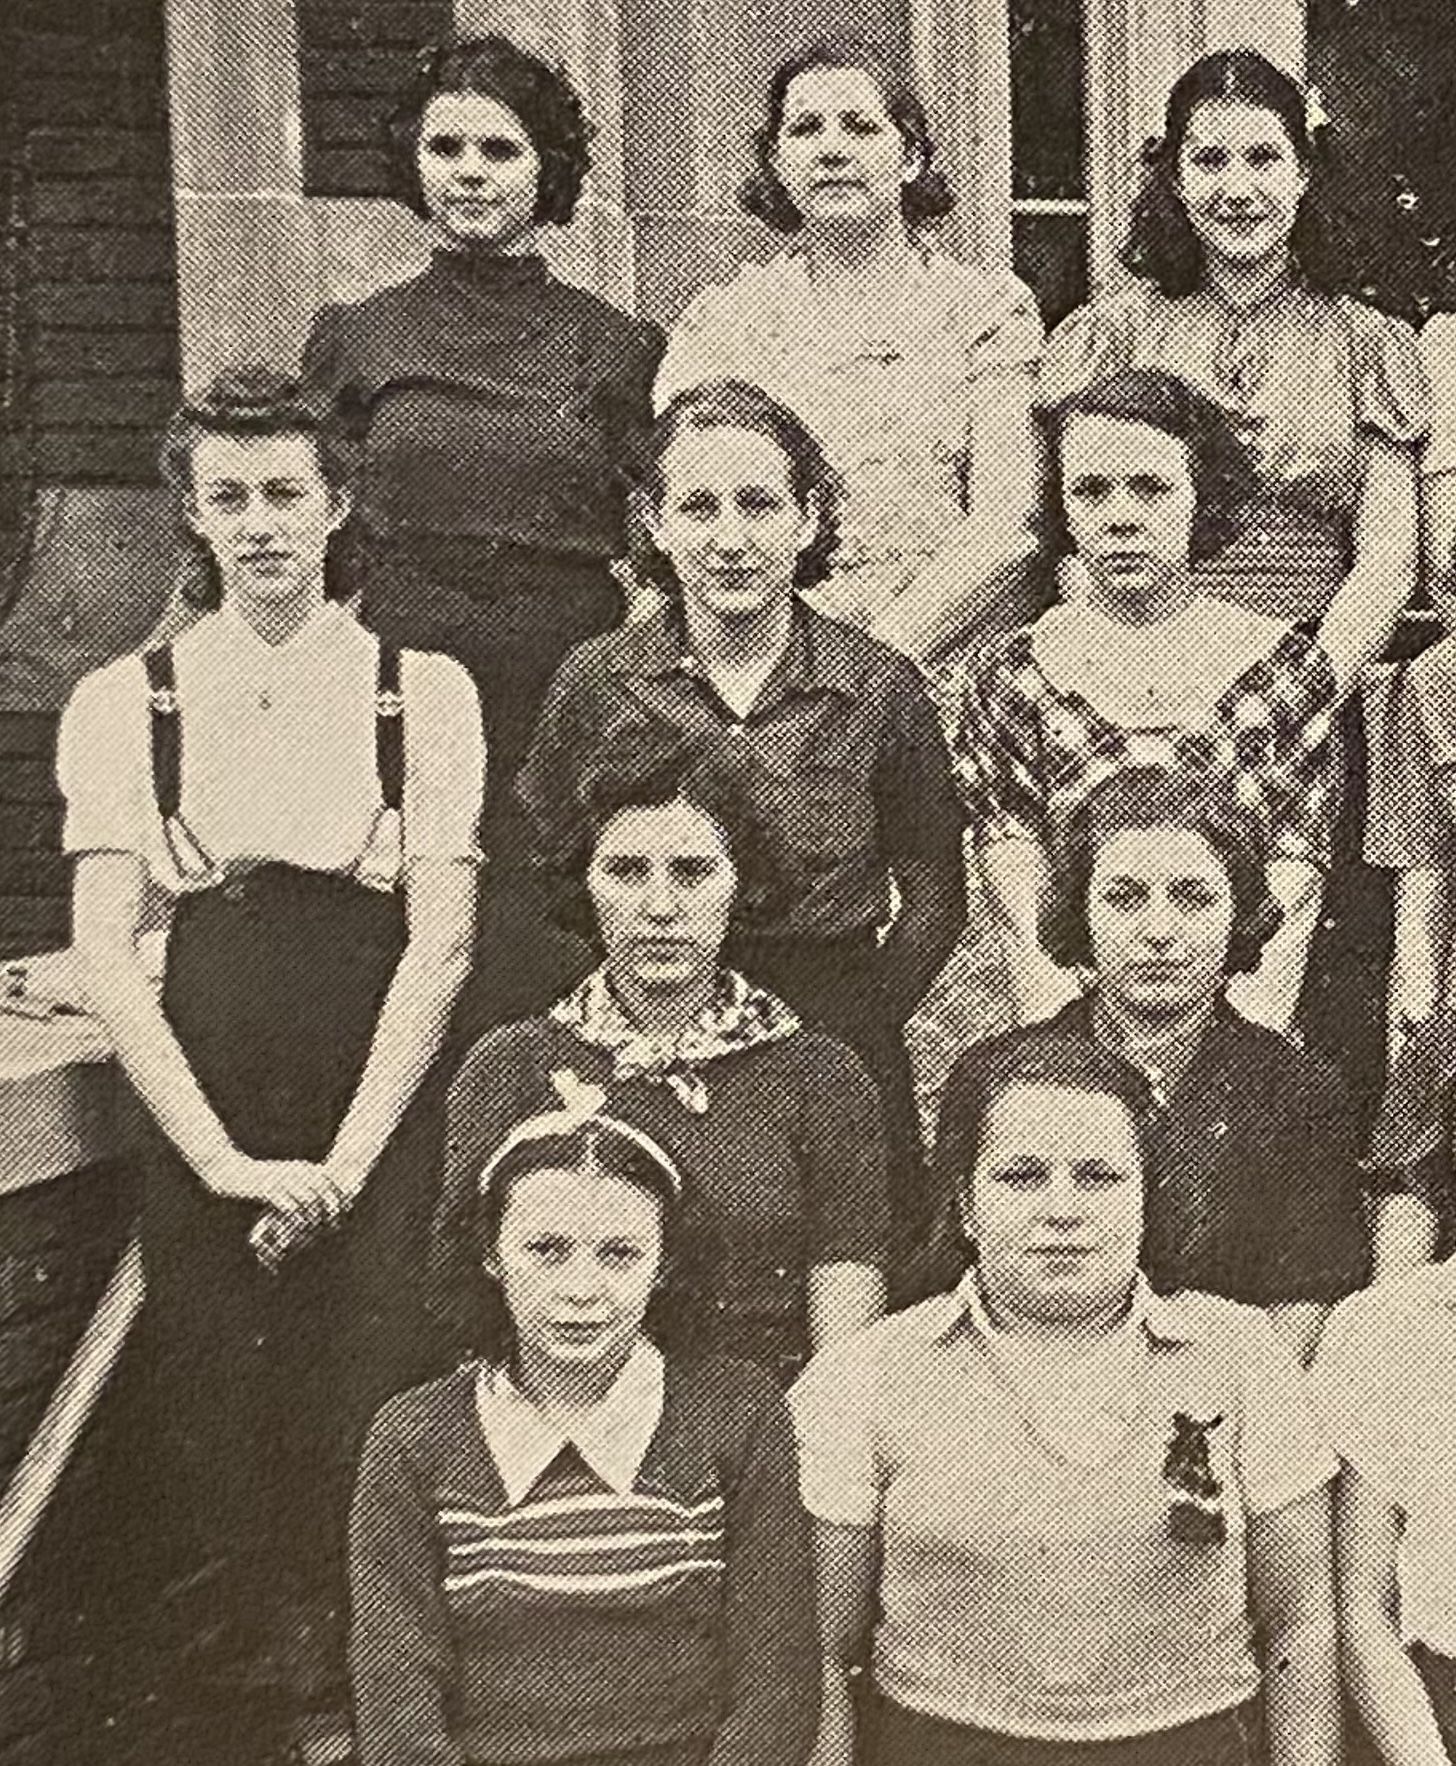
\includegraphics[width=0.7\linewidth,height=\textheight,keepaspectratio]{images/Akou12.jpg}

}

\caption[Lila as a sophomore in 1939 with some of her classmates at
Logan High School]{Lila (middle of the back row) as a sophomore in 1939
with some of her classmates at Logan High School}

\end{figure}%

Looking around at her family, Lila was not sure what kind of life she
wanted to have. Veda had decided to get married instead of becoming a
nurse---was that a good decision? She seemed happy. Her mother had never
worked outside of the home, but she had become a very harsh and bitter
woman. Borgny was happy until Norma Jean got sick and died. Lila
reflected that she wasn't sure if Aunt Hattie was happy or not. She had
been married twice and worked outside of the home, even while married to
Uncle Frank. Lila was intrigued, but the thought of asking Aunt Hattie
for advice gave her a headache.

\section{Notes}\label{notes-22}

Like Veda, my other grandmother (born as Beatrice Englesby) converted to
Catholicism so she could marry my grandfather. Both remained Catholics
and raised their children in the Church. While conversion (and
Protestant-Catholic intermarriage) was a serious concern or even taboo
for many Americans in the early- to mid-20th century, Veda and Lila's
parents were not very religious and did not object to the match or to
Veda's conversion.

I remember hearing my mother and her sisters playfully tease one another
with the name ``Norma Jean.'' I had no idea that she was a real person
who died as a child. Although it must have been painful for Theron to be
partially cut off from the Slaback family (after his role in the death
of his younger brother, Earl), it may have made him a better parent; he
knew the value of life and wanted to do things better than his own
parents had. When Theron died in 1994, he was buried next to Borgny at
Oak Lawn Cemetery.

Although Lila had white privilege, her gender and working-class
background severely limited her career options. Some jobs in La Crosse
were open to women (for example, in the Electric Auto Lite factory);
however, as far as I can tell, Lila's mother and sisters (Izro and Veda)
never worked for pay outside of the home once they were married.

For more information, see Ann K. Finkbeiner\footnote{\citeproc{ref-finkbeiner2012a}{\emph{After
  the Death of a Child: Living with Loss Through the Years} (New York:
  Free Press, 2012)}.}, Claudia Goldin\footnote{\citeproc{ref-goldin2021a}{\emph{Career
  and Family: Women's Century-Long Journey Toward Equity} (Princeton
  University Press, 2021)}.}, David M. Oshinsky\footnote{\citeproc{ref-oshinsky2005a}{\emph{Polio:
  An American Story} (Oxford University Press, 2005)}.}, and Naomi
Schaefer Riley\footnote{\citeproc{ref-riley2013a}{\emph{'Til Faith Do Us
  Part: How Interfaith Marriage Is Transforming America} (Oxford
  University Press, 2013)}.}.

\bookmarksetup{startatroot}

\chapter{Chapter Twenty-Two}\label{chapter-twenty-two}

Veda's wedding was held at Saint James Catholic Church, which was only
one block away from the Riviera Theater; she had been taking classes
there to get the dispensation. Aunt Hattie---who never missed an
opportunity for a good spectacle---offered to take Veda shopping for a
wedding dress. When Veda announced her offer, however, their mother's
face darkened. ``How dare that woman intrude\ldots everyone knows that
the mother of the bride is the one who should handle the dress and
flowers.''

Veda said, ``I'm so sorry! I'll tell her right away that you want to
take care of it.''

The conflict added a sour note to the planning. Even on the day of the
wedding, Hazel was unusually cold to Aunt Hattie. Veda was mortified.
She wanted everyone to be happy. Although they could not afford much,
Veda looked radiant. Thin, with gorgeous hair and a pale complexion, she
would have looked just as beautiful in a flour sack.

Lloyd had been released from prison, but he had not returned to La
Crosse right away. To everyone's surprise (and Aunt Hattie's dismay), he
turned up at Veda's wedding reception. Lila was eating when Lloyd crept
up behind her and whispered, ``Hey beautiful, where have you been all my
life?'' Lila blushed and turned to look at him. He was thinner than the
last time she saw him (before he went to live in Winona) but still
handsome. No other man had ever talked to her like Lloyd. She felt a
rush of excitement. Lloyd asked if they could go somewhere to talk and
she agreed. She pretended like she was getting up for a second helping
and then snuck out the kitchen door. Lloyd suggested that they walk down
to the river so he could have a cigarette. He offered one to Lila, who
politely declined.

As Lila had imagined, the last few years had been difficult for Lloyd.
He talked about what it was like in prison: the mice, the terrible food,
being cold all the time, the concrete walls and scratchy clothes
infested with lice, and worst of all, never knowing what the guards or
other prisoners might do. During his second year in prison his cellmate,
Robert, was stabbed to death during an argument. Lloyd said he had
forgiven the shop owner and the police and attorneys, but nobody would
give him a fair shake at another job. What was he supposed to do with
the rest of his life? Lila listened carefully. She couldn't do much to
help Lloyd, but she could listen. She found it flattering that he
trusted her. Lloyd's life was even worse than her own.

Then he paused and said, ``Enough about me\ldots how has life been
treating you, gorgeous? The boys must be flocking to your door by now.''
Lila blushed. She didn't realize that Lloyd was gauging her experience
(or lack of experience) with men. It was so rare that anyone asked her,
``How are you doing?'' How was she supposed to respond? They had walked
all the way to the river and were sitting on a large limestone rock near
the Clinton Street bridge. They could hear the constant stream of cars
and trucks driving past.

Lila was still thinking of what to say when Lloyd leaned over and kissed
her. It was her first time being kissed and she really didn't know what
to think. Lloyd pulled back to see her expression and must have liked it
because he leaned towards her again and gave her a longer kiss. His
hands were warm on her cheeks. To her astonishment, she felt him
reaching his tongue into her mouth. What in the world was going on? He
pulled back again and smiled. ``Now what was it you were saying?'' Lila
blushed. She truly had no idea what to say. Should she tell him about
her mother's drinking problem or the endless years of chores\ldots or
how she had decided that it was time to drop out of school? Would he
advise her to get married and stop being silly? She didn't think so, but
she was feeling apprehensive about getting advice from the family, even
from Lloyd. She held out her hand and said, ``I guess we should walk
back now.''

Two blocks from the church, Lloyd said he had to go. He was meeting up
with some friends. ``I'll look for you another day; don't worry,'' and
with a smile, he turned. Lila waved. Aunt Hattie had noticed her absence
and asked where she had been.

``I just needed some fresh air, so I took a little walk.'' It was not
entirely a lie.

Aunt Hattie gave her a skeptical look and said, ``You missed the serving
of the cake.''

Thankfully, Allene came to her rescue and said, ``There you are! Come
dance with me. Lyle says that he's tired, but I'm just getting
started.'' One of Red and Veda's co-workers was a fiddler, and he had
agreed to gather a small band to play at the reception. It was turning
into a lively evening.

\section{Notes}\label{notes-23}

I'm not sure what church Veda and Red attended, but Saint James was a
real church located just one block away from the Riviera Theater. In my
experience, weddings tend to draw out the best behavior from people, but
also the worst behavior. It is not hard for me to imagine tension over
who would pay for the critical pieces of a wedding, like the bride's
dress.

Like Lila, I received some inappropriate attention from male relatives
when I was a teenager. Weddings are chaotic (especially receptions) so
that gives predators unusual opportunities. I have no idea if Lloyd was
a predator or not, but some family members were. My first ``French
kiss'' was foisted on me by a relative who is no longer alive. He would
have done more if I had not carefully avoided him for the rest of the
event.

During the Great Depression, many families in rural areas saved money by
making clothing out of feed sacks and flour sacks, which were often
printed with paper labels or ink that could easily be washed out. Lila
might have seen flour sack dresses when visiting extended family.

For more information, see Vicki Howard\footnote{\citeproc{ref-howard2008a}{\emph{Brides,
  Inc.: American Weddings and the Business of Tradition} (Philadelphia:
  University of Pennsylvania Press, 2008)}.}, Samanta
Leonard\footnote{\citeproc{ref-leonard2019a}{\emph{Groomed: Shining a
  Light on the Unheard Narrative of Childhood Sexual Assault}
  (Washington, DC: New Degree Press, 2019)}.}, and Susan
Miller\footnote{\citeproc{ref-miller2007a}{\emph{Vintage Feed Sacks:
  Fabric from the Farm} (Lancaster, Pennsylvania: Schiffer Publishing,
  2007)}.}.

\bookmarksetup{startatroot}

\chapter{Chapter Twenty-Three}\label{chapter-twenty-three}

True to his word, it was not long before Lloyd returned. One day Lila
was walking to her new job (she had answered an ad looking for a ``girl
for general housework''), and there he was, perched on the edge of a
stone wall, smoking a cigarette. It was October and the trees were flush
with orange and yellow leaves. One leaf had fallen on Lloyd's head, and
Lila playfully brushed it off.

``Hey, that was my hat,'' said Lloyd. They both laughed. ``What do you
say we go to my place?''

Lila was curious to see where Lloyd was living but said, ``Mrs.~Davis
will fire me for sure if I'm late for work again.''

With a grin, he replied, ``I'll be waiting when you finish.''

For several days, Lloyd waited for Lila until she finished work. All she
wanted to do was walk home, eat dinner, and get some sleep, but Lila
appreciated having someone to walk with. Lloyd treated her like a real
adult and told the funniest jokes, although his language would have made
most women blush (even most men). Lila had never done anything so
exciting and dangerous. Spending time with Lloyd was her first major act
of rebellion against her parents and Aunt Hattie. She decided that on
Saturday she would go with Lloyd to see his place; she could tell her
parents that she had been at the movies. Lloyd gave a cowboy ``Yahoo!''
when she told him, and he practically skipped all the way to Rose
Street.

As they approached the boarding house, Lloyd said, ``When we go in, just
follow me and don't talk to anyone.'' It was dim and chilly inside.
There were mailboxes and a small desk near the front door. ``Good, the
desk is empty tonight. I swear that woman thinks we're just a bunch of
good-for-nothing children\ldots{}'' Lloyd took Lila's hand and led her
towards a flight of stairs. As they went upstairs and approached a door
in the middle of the hallway, he pulled a key out of his coat pocket.
``This is the one!'' Lila was not expecting much, but Lloyd's room was
worse than she had imagined. The floor and walls were bare, and the room
was just barely large enough for Lloyd's bed; in the corner, there was a
pile of laundry and some empty bottles. His bed was not made, and it was
loosely covered with a ragged gray blanket. Lila could hear someone
moaning in the next room. He shut the door and hung his coat on a big
nail. ``I know it's not much, but the view sure improved when you walked
in.'' The condition of the building and its occupants made Lila feel
sick to her stomach, but she tried not to show it. She was an adult now.

Lloyd slipped off her coat and laid it over the edge of the bed. It was
navy blue wool, but in the dim light it looked black; without her coat,
it was quite chilly in Lloyd's room.

``Where do you go to the bathroom?''

``Oh\ldots just down the hall. Sometimes when I'm too lazy, I piss in
one of those bottles.''

Lila was imagining what it would be like to piss in a bottle (being a
woman, it was something she had never considered) when Lloyd put his arm
around her waist. Although he smelled like cigarettes, his body was warm
and reassuring. She had never been so close to a man who was not her
father or brother. Lloyd said, ``I'll try not to hurt you.'' For the
first time, Lila wondered what Lloyd had in mind---it was clearly not
just a tour of his place. He put his hand on her breast and gently
pushed her backward on the bed. Lila immediately realized that this
would be her first sexual experience. She had heard her brothers
whispering about it with their friends, but she felt very unprepared.
Also, Lloyd was her cousin. Everyone knew that cousins were not supposed
to do this kind of thing. She uttered, ``Lloyd, I don't\ldots{}'' but
Lloyd whispered, ``Don't worry beautiful, I'll take good care of you.''
As his breathing grew louder and faster, she was surprised to find that
hers was too. It was so painful that first time but thrilling in a way
that she had never experienced before. Lloyd was clearly enjoying it.

When Lloyd finished, there was a pool of blood on the sheets. Lila was
horrified. ``I'm so sorry, it must be that time of the month!''

Lloyd chuckled and said, ``That's normal for your first time\ldots don't
worry about it.''

Although she knew the room was nearly bare, she couldn't help looking
around for something to use as a washtub. She knew that if the blood was
allowed to dry it would be nearly impossible to get the blanket clean
again, even with bleach. It was the kind of thing that would make her
mother furious. Lloyd must have noticed her look of rising panic. As she
buttoned the front of her dress, Lloyd put his hands on her waist and
said, ``It's OK\ldots Lila\ldots don't worry about it.'' A tear spilled
and rolled down her cheek. She felt like a child for crying, but she
couldn't help it. Lloyd gave her a hug and said, ``I'll walk you home.''

For several weeks, Lloyd was waiting for her nearly every day. One day
he surprised her with a beautiful scarf. It was so soft---pink, with red
roses in the center. Lila had never owned anything so gorgeous, but she
didn't ask where it had come from. Lloyd had secrets. To keep her mother
from noticing, she hid the scarf under her mattress. Another time, he
gave her a bouquet of real roses. The smell was divine, and the petals
felt like heavy silk, but Lila giggled, ``What am I supposed to do with
these?'' On the way back to her neighborhood, they took a stroll through
Oak Lawn cemetery and laid the roses on Norma Jean's grave.

One night Lloyd said, ``You're the best thing that ever happened to me,
Lila. I wish we could be together like a real married couple.'' Lila was
ambivalent. She had grown very attached to Lloyd, but did she really
want to get married? She had stumbled into a relationship that was
starting to seem like an ideal: affectionate and fun, but with no
strings attached. One of the best things about being with Lloyd was that
they could never get married. As much as she wanted to be an adult (and
she was), the thought of starting a family and becoming a housewife
filled her with dread. She never dared to ask him if he wanted to get
married or what he thought marriage would be like. It was not a
relationship that involved deep discussion.

\section{Notes}\label{notes-24}

For this chapter, I scoured classified ads in the \emph{La Crosse
Tribune} to see what kinds of jobs were available to young women in
1941. Lila was getting too old to work as a child minder, but she did
not have any special qualifications or training. The most common
advertisements were for housekeepers (domestic servants), both part-time
and full-time. Although many households in major cities like Boston,
Philadelphia, and Chicago were hiring Black women by the 1930s and
1940s, La Crosse was a sundown town. Regardless of race, the pay was
extremely low because domestic servants were excluded from the Fair
Labor Standards Act of 1938.

As an alcoholic and recently released prisoner, Lloyd's options for
housing would have been extremely limited. I have no idea where he lived
when he was not in prison, but he might have lived in a boarding house
or a halfway house. Although marriages between cousins are allowed or
even encouraged in some countries, they are generally illegal in the
United States.

For more information, see Ellen C. Kearns and Monica Gallagher,
eds.\footnote{\citeproc{ref-kearns1999a}{\emph{The Fair Labor Standards
  Act} (Washington, DC: Bureau of National Affairs, 1999)}.},
Loewen\footnote{\citeproc{ref-loewen2018a}{\emph{Sundown Town}}.},
Martin Ottenheimer\footnote{\citeproc{ref-ottenheimer1996a}{\emph{Forbidden
  Relatives: The American Myth of Cousin Marriage} (Champaign:
  University of Illinois Press, 1996)}.}, and Phyllis Palmer\footnote{\citeproc{ref-palmer2010a}{\emph{Domesticity
  and Dirt: Housewives and Domestic Servants in the United States,
  1920--1945} (Philadelphia: Temple University Press, 2010)}.}.

\bookmarksetup{startatroot}

\chapter{Chapter Twenty-Four}\label{chapter-twenty-four}

On the first Saturday in December, Hazel went to a holiday banquet held
by the Royal Neighbors of America; it was one of the organizations she
had joined after Aunt Hattie insisted that she needed to stop drinking.
Lila didn't know much about it, but she was grateful to make dinner in
peace and quiet. Lila and Looy were the last two siblings living at
home, and Lila was taking the brunt of her mother's never-ending
criticism. ``Look at this spot you missed when you were mopping. Why is
the meat raw in the center? Why are you cleaning the windows with that
filthy rag\ldots didn't I teach you better?'' Between her paying job and
doing the chores at home, Lila was exhausted. Her knees and shoulders
ached like the joints of an old woman. Her hips were so sore at night
that the constant pain often woke her up.

When Hazel entered the front door, John and Looy were sitting in the
living room, and Lila was setting the table. ``You won't believe the
gossip I heard tonight: Lloyd was arrested again for burglary.'' Lila
dropped the pitcher of milk she was carrying. Hazel barked, ``What is
wrong with you, Lila? You're so careless these days.'' Lila said
nothing. She looked down at the broken pottery and the pool of milk
spreading over the floor. ``Get a rag and clean that up.'' As Lila got
to work, her mother told the rest of the story. Lloyd's picture had been
all over the newspapers; he was running with a gang of three men, and
they had stolen some liquor and cash from the labor temple. ``When is
that fool going to learn his lesson about prison?'' Lila felt like she
had been kicked in the stomach, but there was nothing she could say or
do.

The next day as they were doing laundry, her mother said, ``You know,
Lila\ldots when I was nineteen, I was already married with a child on
the way. Men can wait to get married, but women don't stay young
forever.'' Lila sighed. It was not the first time this topic had come
up. Now that Veda was married, her mother was on a mission to get Lila
married. But as much as she looked forward to getting out of the house,
Lila had no real interest in marriage. Where was she supposed to find a
potential husband? The usual way to meet someone was at school or at a
party, but Lila was out of school, and she was rarely invited to
parties. She didn't have much time for anything besides work, chores,
and spending time with Lloyd.

Aunt Hattie was trying to play matchmaker. It had worked for Theron,
Izro, and Lyle. She had invited Lila to her house several times for tea,
but Lila knew what that meant and kept refusing to accept. It was a
quiet thrill to frustrate Aunt Hattie. Couldn't the family just wait for
a few years and let her figure things out on her own? Veda had found her
own match.

A few days later, Hazel announced that she wanted to host a gathering
for the Service Star Legion. After the shocking attack on Pearl Harbor,
families with sons in the military could use their support. When Lila
said that she would be willing to help cook and serve the food, her
mother said, ``Wonderful, we can plan the menu together.'' Lila and
Hazel cleaned the house from top to bottom, and Aunt Hattie allowed them
to borrow her good dishes and tea service. Lila expected that they would
prepare a full dinner (and was already fantasizing about the different
types of pies she could make), but her mother said that finger foods
would be easier to make and serve. They settled on tiny sandwiches
filled with cream cheese and ham, deviled eggs, Swedish meatballs, cubes
of Jell-O, sugar cookies, and mulled cider. When it was too dark to play
outside with his friends, Looy helped the effort by setting up a small
Christmas tree and making strings of popcorn and paper chains to
decorate the walls. When the table was full and they were waiting for
the guests to arrive, Lila had to admit that the house smelled and
looked wonderful. She felt proud to serve her patriotic duty.

Much to Lila's surprise, her mother had given her a tube of lipstick
that morning. She had often wished that she could have ruby lips like
Scarlett O'Hara, but Hazel didn't wear lipstick or any cosmetics at all;
receiving such a gift was like suddenly discovering that your pet dog
could dance the polka. Her mother had pressed the tube into Lila's hand
and walked away, giving her no opportunity to ask questions. The night
before the party, Lila had carefully set her hair into a wave; wearing
the lipstick and her best dress, she felt quite glamorous. Looy was
going to help serve their guests; he had been ordered to take a bath and
put on some clean clothes and to carry around trays of hors d'oeuvres.
It was funny to see him dressed up like he was going to church; it was
not Looy's usual state of being.

Many of the guests lived in their neighborhood. Lila recognized some of
the families of her classmates. Marius and Snorre Gronbeck had dropped
out of school the year before to join the military; Marius was in Lila's
class. Their parents were Norwegian and spoke English with heavy
accents. Lila wondered if they felt like they had to ``prove''
themselves as Americans. It was not something she had considered when
Marius announced that he was leaving. Most of the people who attended
the party were parents, sisters, and younger siblings. There were also a
few young men who were home on leave or getting ready to enlist. When
Lila saw Earl Bright (who was a few years older; he had been one of
Cecil's classmates), she assumed that he fell into one of those
categories; he said he was visiting from Illinois.

As they were talking, Aunt Hattie passed by with a smirk on her face.
Earl asked if they could go for a walk, and Lila went to get her coat
and mittens. It was a clear and very cold night. As they walked, Earl
pointed to Orion, the north star, and the big and little dipper. Lila
was not impressed; everyone knew those constellations. Earl said he was
going to enlist in the Navy as soon as the holidays were over. His nose
was turning progressively red from the cold. Lila was on the verge of
laughing when he said, ``I guess we better turn back. I didn't realize
it would be so cold tonight!'' He was so boring. That night, Lila fell
asleep thinking of Lloyd. The last time he had walked her home from
work, he told her a joke about a married couple:

\begin{quote}
A man tells his wife that he needs to go buy a pack of cigarettes. He
goes to the bar at the end of the block, sees a beautiful woman, one
thing leads to another, and they end up going to her place. As soon as
the fun is over, he falls asleep. He wakes up and realizes, ``Shit, I
don't even have cigarettes! What am I going to tell my wife?'' He leaps
out of bed and runs outside to rub his shoes in the grass and mud. He
goes home, and his wife is still awake.

``Where have you been?'' she says furiously.

The man says, ``You won't believe it, honey\ldots I went to the bar to
buy some cigarettes, but I saw a beautiful woman and we ended up going
back to her place and having sex.''

The wife looks down at his shoes and says, ``You lying bastard! You went
fishing again!''
\end{quote}

It made her smile just thinking about Lloyd and his scandalous jokes.
She wondered how long it would be until they could see one another
again. Maybe he wouldn't be sentenced to prison after all. Maybe the
police had made a mistake. She pulled the scarf out from under her
mattress and fell asleep with it pressed against her cheek.

The next day there was a knock on the door: it was Earl and his parents.
Lila was in the kitchen washing the enormous stack of dishes from the
party when she heard, ``Lila dear, please come out here.'' Her mother
never said ``dear.'' She reluctantly dried her hands and walked to the
living room, still carrying the dish towel. When Earl saw Lila, he
dropped to one knee and said, ``Lila, I've come to ask for your hand in
marriage.'' He opened a tiny box with a ring inside---it had a thin band
of gold with a square ruby and two tiny diamonds.

\begin{figure}[H]

{\centering 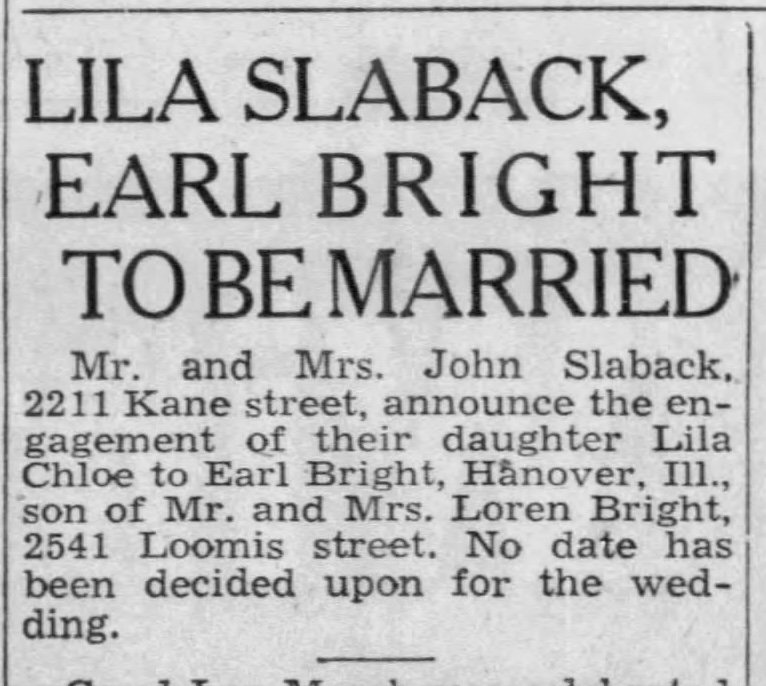
\includegraphics[width=0.55\linewidth,height=\textheight,keepaspectratio]{images/Akou13.jpg}

}

\caption{Page 4 of the \emph{La Crosse Tribune}, December 30, 1941}

\end{figure}%

Lila's heart dropped. She hardly knew Earl. What was the rush? As if
reading her mind, her mother said, ``Earl wanted to propose before he
leaves for the war.'' Earl took the ring out of the box and slipped it
onto her left hand. The band was a little too big, and the ruby drooped
to the side; for months, the prongs would dig into her pinky finger,
reminding her of that painful and awkward moment. As Lila stood there
silently, the room erupted in happy chatter.

``Earl is leaving for Illinois\ldots{}''

``Lila can live with us\ldots{}''

``I'll send an announcement to the newspaper first thing in the
morning.''

Wasn't she supposed to say yes, or no? Earl gave her a peck on the cheek
and his parents began putting their coats back on. Lila was stunned.
Aunt Hattie was the one who put the announcement in the newspaper.

Lila knew it was cruel, but she hoped that Earl would be killed in the
war. Veda told her it was so exciting to marry a soldier going off to
war! Just like a movie. But Lila didn't want to plan a date for the
wedding. A few weeks later, Lloyd was sentenced to serve up to five
years in the state prison. Lila wondered what her life would be like in
five years. Would she be married to Earl? Would she have children? It
was gut-wrenching to think how quickly her life had turned for the
worse. She had been happy with her life the way it was.

\section{Notes}\label{notes-25}

Following the attack on Pearl Harbor, the rate of engagements and
marriages in the United States tripled as young couples rushed to
formalize their relationships. Lila was approaching the average age for
a first-time marriage in the 1940s (twenty-one for women, twenty-four
for men), but I imagine that her parents also wanted to be done with the
hard work of raising children.

Although I grew up in a later time (the 1980s and 1990s), I remember the
confusing push-pull of becoming an adult. Don't get pregnant! But
also\ldots get married and have children! I used yearbooks to find names
of Lila's actual classmates, then searched for them in the
\href{https://aad.archives.gov/aad/index.jsp}{National Archives
database} to see who had served in the war.

I found Lila's engagement announcement in the \emph{La Crosse Tribune}.
I was stunned because I had never heard of Earl Bright. He might have
been a ``good catch'' in the eyes of Lila's family, but was he
compatible? I have no idea what Earl was like; the contrast with Lloyd
is striking.

The Internet is full of historical examples of jokes; I just adapted one
that I thought was especially appropriate for Lloyd and Wisconsin.

For more information, see Bailey\footnote{\citeproc{ref-bailey1989a}{\emph{From
  Front Porch to Back Seat}}.}, Kenneth Rose\footnote{\citeproc{ref-rose2012a}{\emph{Myth
  and the Greatest Generation: A Social History of Americans in World
  War II} (New York: Routledge, 2012)}.}, and Carol Wyman\footnote{\citeproc{ref-wyman2001a}{\emph{Jell-o:
  A Biography} (San Diego, California: Harcourt, 2001)}.}.

\bookmarksetup{startatroot}

\chapter{Chapter Twenty-Five}\label{chapter-twenty-five}

Veda and Red were living with his uncle until they could afford a house
of their own. Since they were both working, it was just a matter of time
until they could save enough money for a down payment. They had come
over for dinner and made their announcement as Lila was bringing out the
dessert (a beautiful yellow cake with white icing). Veda blushed and
said, ``I guess I won't be able to work for much longer.'' Lila looked
at her belly but couldn't see any difference. How did Veda know she was
pregnant?

John cleared his throat and said, ``We have some news too.'' He turned
to Veda and said, ``Since Lila is getting married, your mother and I
have decided to move. You and your husband can move in here. Lila should
stay until the wedding and then the house will belong to you.''

Red said, ``That's very generous, but I can take care of my wife. We're
looking at houses in the neighborhood and nearly have enough money
saved.''

Hazel snapped, ``Don't be stupid. This will give you a proper home for
my grandchild and you can use the money for something else.''

They all ate their cake in silence. Their parents never explained why
they had decided to move, but Lila suspected that her mother was the
driving force: she hated living in the city. They also never explained
their decision to give the house to Veda and Red. Cecil and Gladys were
living upstairs at Lyle's house and were expecting a baby too\ldots why
not them? Why not herself? She had no idea where Earl might want them to
live, but his parents lived in La Crosse, and it was reasonable to think
he would return after his service. Maybe her parents were worried that
he wouldn't survive or would not want to inherit their house.

Lila wrote a letter to Earl and told him about the plan. Lyle and Cecil
were going to help her father build a new house out in the country. He
had purchased a small plot of land between La Crosse and
Onalaska---enough to have a big garden and some distance from neighbors,
but not enough to farm for a living. It was a short letter; she didn't
love Earl and had no idea what to say. Hope you survive the war? She
hadn't received any letters from him---she assumed life in the Navy was
keeping him busy. Spontaneously, she decided that she would also write a
letter to Lloyd. Could prisoners receive letters? She wasn't sure but
imagined how much it would cheer Lloyd up to receive a letter from her.

\begin{figure}[H]

{\centering \pandocbounded{\includegraphics[keepaspectratio]{images/Akou14rt.jpg}}

}

\caption[Postcard of Wisconsin State Prison in Waupun]{Postcard of
Wisconsin State Prison in Waupun, where Lloyd was sent in the 1940s}

\end{figure}%

\begin{quote}
February 3, 1942

Dear Lloyd,

I was so sorry to hear about your arrest. I don't know if you will get
this letter, but I miss you and think about you every day. Veda is
having a baby. My parents are moving out into the country. Life is
boring without you. I go to work, and I come home and do more work. I
miss our walks together and your funny jokes. Maybe you will learn some
new jokes while you're away.

Love, Lila
\end{quote}

She put on some lipstick and kissed the bottom of the letter by her
name. Later that week she went to the post office to buy stamps. She
addressed the envelope to ``Lloyd Slaback, Waupun Prison'' and slipped
it into one of the mailboxes. Would that be enough? She had no idea but
resolved that she would write to him every week.

One day while she was at the post office she bumped into her former
classmate, Myrtle Johnson (now Mrs.~Carl Schneider). Myrtle noticed the
engagement ring on Lila's left hand and squealed, ``Ooh, Lila, I'm so
happy for you! Who is the lucky man?'' Lila was still holding a letter
addressed to Lloyd and hoped that Myrtle hadn't seen the name. Lila
blushed, and Myrtle squealed again and gave her a hug.

``His name is Earl and he's in the Navy.''

Myrtle said, ``Well that's a coincidence, Carl just left a few weeks ago
to join the Navy. That makes us practically sisters! You should come
over for tea\ldots we have so much to catch up on.''

Unable to think of a good excuse, Lila said, ``Sure, that sounds
lovely.''

Myrtle wrote her address and phone number on the back of a stray
envelope and handed it to Lila. ``Don't be a stranger. I'm bored to
tears keeping house while Carl is away.''

Lila promised that she would drop by on her next day off. They had never
been close friends, but it would become one of the most important
friendships of Lila's life, giving her options when she thought there
were none left.

As soon as the snow melted, Lila's father and brothers began building
her parents' new house. Lila moved her things upstairs so Red and Veda
could have the small bedroom. As soon as her parents moved, they would
shift to the larger bedroom and Lila could have the small one again. It
was embarrassing to be almost twenty years old and sharing a room with
your brother, even if it was just temporary. Lila nailed three sheets to
the rafters to make a little bed chamber and told Looy that she better
not catch him snooping.

``Oh yeah, so what if I do?''

Lila snarled, ``Do you really want to find out?''

Looy ran off saying, ``Oooh\ldots I'm really scared,'' but he was
thirteen and just as embarrassed to be sharing the room.

Veda was now visibly pregnant. Although she insisted that she was ``just
pregnant, not sick,'' Hazel demanded that she take it easy. The two of
them started going through the house, making decisions about what to
move and what to leave. Veda and Red had clothes (of course) and had
received some household necessities as a wedding gift---towels, sheets,
pots and pans, etc.\ldots Aunt Hattie had given them a small, but very
beautiful set of china. Red's father had given them a little money. He
also made a cutting board that so was smooth and lovely; Lila didn't see
how Veda would ever stand to use it for its intended purpose. Hazel said
that they would leave most of the furniture. In the attic, they still
had Looy's cradle. ``Oh, that will be perfect when the baby arrives,''
said Veda. As Lila continued doing most of the cooking and cleaning,
Veda made diapers and clothes for the baby using Hazel's treadle sewing
machine.

The house was getting busy again. Veda's friends organized a baby shower
and asked Lila to make the desserts. A steady stream of acquaintances
dropped in to tell Hazel how sorry they were to see her go. She loved
the attention and treated Lila like a maid, ``Go fetch us some
sandwiches. Take these plates to the kitchen. Go get Mrs.~Taylor's
jacket from the bedroom.'' It was so much work that she started to think
about quitting her job with Mrs.~Davis. Cleaning and cooking around the
clock was taking a toll on her knees and back.

\section{Notes}\label{notes-26}

Although my sister is a little younger than I am, she was the first one
to get pregnant. Like Lila, I wondered how she knew. She didn't look any
different.

In 1949, Lloyd married a woman named Lilah who had been married at least
twice before. It took months for me to realize that Lilah Slaback in the
phonebook was not ``my'' Lila.

In this chapter, we are reintroduced to Myrtle Johnson (now Myrtle
Schneider), who is thrilled to be married and wants the same joy for her
friend, Lila Slaback. Family members have described Myrtle to me as
``Lila's best friend,'' but I wonder if they felt equally committed.
Before I wrote this book, I had no idea that they were classmates in
high school. When did they first become friends? As an adult, I have
realized that friendships can easily grow and shrink in importance. As a
child, I knew Myrtle as ``Grandma Schneider.'' I knew what she was like
as a person and can still imagine her voice in my head.

Like Lila, my parents moved out of my childhood home when I was twenty,
just after I got married. I had lived there since I was a toddler and I
found it really unsettling to lose my ``home'' (even though I had moved
out and did not intend to live there again). The moving process brought
up all kinds of difficult feelings surrounding what to keep or get rid
of and who should have it (me, my sister, or my parents).

For more information, see Jennifer L. Adams\footnote{\citeproc{ref-adams2023a}{\emph{An
  Autoethnography of Letter Writing and Relationships Through Time:
  Finding Our Perfect Moon} (New York: Routledge, 2023)}.}, David
Celani\footnote{\citeproc{ref-celani2011a}{\emph{Leaving Home: The Art
  of Separating from Your Difficult Family} (New York: Columbia
  University Press, 2011)}.}, and Sheila Isenberg\footnote{\citeproc{ref-isenberg2021a}{\emph{Women
  Who Love Men Who Kill: 35 True Stories of Prison Passion} (New York:
  Diversion Books, 2021)}.}.

\bookmarksetup{startatroot}

\chapter{Chapter Twenty-Six}\label{chapter-twenty-six}

Veda's baby, whom they named David, was born just a few days after the
new house was finished. Lila thought her parents might wait a few weeks
before moving so Hazel could help Veda and they could spend a little
time with their new grandchild, but Hazel was clearly anxious to get
going. Since there was no high school near their new house, and it was
too far to drive to La Crosse or Onalaska on a daily basis, the family
had decided that Looy would stay behind and live with Veda and Red. As
they all said their goodbyes at the curb, Veda promised that they would
be up for a visit soon. And that was that. Lila had helped pack their
belongings in the back of Theron's truck; on the first day of summer,
they drove off.

Although Lila had been in the house on Kane Street plenty of times
without her parents, it was strange knowing that they would no longer be
living there. They had all known that this day was coming, but Red and
Veda seemed to be in shock. Were they really the owners of this house
now? Veda went back to taking care of the baby, and Red went back to
work. Veda was not as demanding as Hazel. Lila was glad that she had not
quit her job after all.

One night at dinner a few weeks after their parents had moved, Veda
announced that it was time for all of them to start going to church on a
regular basis. David should be baptized as soon as possible; it would be
a blessing for them to go to confession on Saturdays and mass on
Sundays. Lila inwardly groaned---the Slabacks were not churchgoers. Why
did Veda have to be in charge?

Looy said, ``Do I really have to go?''

Without hesitation, Red calmly answered, ``As long as you're living in
my house, yes you do.''

That summer Lila finally received a letter from Earl, but it was not the
kind of news she had been expecting.

\begin{quote}
August 2, 1942

Dear Lila,

I should have written to you earlier, but I wasn't sure what to say.
When I tried to join the Navy, they told me I had a heart murmur, so I'm
``not eligible'' to join the service. Can you believe that? I thought
they would take anyone right now.

I've been living in Illinois and working as a truck driver. There's no
easy way to say this, but I've met someone else. Her name is Aline. We
got married, and we're planning to move to La Crosse in a few months. I
didn't want you to find out from someone else.

I'm sorry that things didn't work out between us. You seem like a nice
girl. Please keep the ring. You can sell it if you need to.

Sincerely, Earl
\end{quote}

Lila knew the family would be upset, but she was relieved. She had never
agreed to get married and now she didn't have to say yes or no. The
wedding was off. She tucked the letter under her mattress and decided to
think about how she was going to tell everyone. Would her mother and
Aunt Hattie start pressuring her again? She was grateful that she had
been the one who checked the mail that day. Nobody else knew of the
letter's existence.

After a few weeks, she decided to break the news to Veda. It was Lila's
day off and Red was at work. They were sitting in the front room
watching the baby as Veda worked on knitting him a sweater. ``Veda, I
have something to tell you\ldots I'll be right back.'' She retrieved the
letter from Earl, which was looking rather crumpled after all of the
times Lila had read it, and stuffed it back under her mattress. ``I need
your advice about something. I want you to listen and then take a moment
to think before you say anything.'' Veda stopped knitting as Lila read
the letter out loud.

She stared at Lila and opened her mouth, but for a few moments, nothing
came out. ``What are you going to tell mom and dad?'' Veda asked.

Lila said, ``I have no idea! It's not my fault that Earl married someone
else. It wasn't even my idea to get engaged in the first place.''

Veda said, ``Calm down, Lila, of course you wanted to marry Earl. Don't
exaggerate. I just don't know how you're going to tell Mom or find
another man to marry. You should tell Aunt Hattie.''

Lila was shocked. She didn't think Veda was trying to be mean, but was
that really her best advice? Lila said, ``I need to wash the dishes
now,'' and walked away.

Telling Myrtle was not much better. She burst into tears like Earl had
died. Lila didn't tell her that she had never wanted to marry Earl.
After Veda's reaction, she had decided that it was probably best to keep
that information to herself. Through her tears, Myrtle said, ``I don't
know why I'm the one who's crying\ldots I should be comforting you.''
Lila gave her a little hug. Why did this have to be so hard? She wasn't
even sure she wanted to get married, but everyone was acting like her
life was over unless she could get engaged again. It seemed to be the
only thing anyone cared about. After a few minutes, Myrtle went into the
kitchen for another plate of cookies. ``We just need to find you another
man. That will make everything better. In a few months, we'll say, `Earl
who?' and laugh about the whole thing!'' Lila doubted that was true.

With the wedding off and Lloyd in prison, Lila decided to become a
regular at the movie theater. The price of tickets had increased by
three cents, but it was bliss. No chores, no talk of ``finding a man,''
just a box of popcorn and two hours of escape. She skipped \emph{I
Married a Witch} based on the title but watched everything else---war
movies, cartoons (\emph{Bambi} was popular that fall), science fiction,
mysteries, dramas---she enjoyed them all. The comedies were her
favorite. The first time she saw Claudette Colbert was that year in
\emph{The Palm Beach Story}. What a smart and funny woman! When her
husband couldn't provide for her, she didn't sit around moping about it.
She took matters into her own hands and left to find an exciting new
life. Lila was still wearing the ring from Earl, but she took it off
that night.

\section{Notes}\label{notes-27}

When my friends started having babies, I was fascinated (and frankly, a
bit jealous) at how some grandmothers joyfully spent weeks or even
months helping their daughters and grandchildren. I did not have that
kind of support. My mother and her mother did not either. Lila probably
came from a long line of mothers who were neglected and marginalized by
society.

The 1943 phonebook lists John and Hazel Slaback as living on S. Salem
Rd. Cecil and Gladys were living at the original Slaback house on 2211
Kane Street. I don't know who inherited the house directly, but it
stayed in the Slaback family for some time. I have proof (such as
marriage records from the state of Wisconsin) that Earl married a
different woman, but I'm not sure how his engagement with Lila fell
apart.

In this chapter, Veda is establishing a life for herself as a Catholic
and stay-at-home mother. It is not the kind of life Lila wants for
herself. This is how siblings start to drift apart as adults---not
because they don't care about one another, but because they simply have
different interests and different visions for living a good life. I
don't know if Lila was the avid moviegoer I make her out to be in this
book, but I imagine how films would have presented options (like
divorce) that older members of the Slaback family were unaware of. The
usefulness of their advice was probably very limited at times.

For more information, see Geoffrey L. Greif and Michael E.
Woolley\footnote{\citeproc{ref-greif2015a}{\emph{Adult Sibling
  Relationships} (New York: Columbia University Press, 2015)}.}, Eva
Illouz\footnote{\citeproc{ref-illouz2023a}{\emph{Consuming the Romantic
  Utopia: Love and Cultural Contradictions of Capitalism} (Berkeley:
  University of California Press, 2023)}.}, and Susan K. Pfeifer and
Marvin B. Sussman\footnote{\citeproc{ref-pfeifer2014a}{\emph{Families:
  Intergenerational and Generational Connections} (New York: Routledge,
  2014)}.}.

\bookmarksetup{startatroot}

\chapter{Chapter Twenty-Seven}\label{chapter-twenty-seven}

One day Lila went to work and was shocked when a man answered the door.
``Can I help you?'' he said.

``Yes, I'm here to clean for Mrs.~Davis\ldots is she in?''

The man looked her up and down and said brusquely, ``My mother has
become very ill.~The doctors are not expecting her to survive much
longer\ldots your services are no longer needed here.'' He shut the door
in her face before she could respond. It was the end of the week, and
Mrs.~Davis was supposed to pay her the next day. She knocked on the door
again, but the man didn't answer.

Veda had relented on telling Lila to go to church but did ask her to
``set a good example for Looy.'' On the occasions when she went to mass,
Lila would inevitably look around at the other parishioners and think,
``Is this really my life?'' It was so boring. Lila could have found
another cleaning job but decided that she needed something more
exciting. With the last bit of money she had earned by working for
Mrs.~Davis, she took a streetcar downtown to purchase a dress and a new
pair of shoes. Her usual ``housedress and apron'' was good enough for
cleaning, but it was not going to help her land a job as a waitress.
With the war going on, many young women were working as waitresses;
there weren't enough men to fill all of the jobs and it was becoming
much more socially acceptable. Lila had already stopped at five places
to inquire if they were hiring, but they all said something like,
``Sure, leave your phone number and we'll give you a call.'' Lila didn't
have a phone or a phone number.

The first place she went to look for a dress was Doerflingers, but she
felt so conspicuous. She walked up the stairs to avoid the elevator man.
When the sales staff asked if she would like any help, she politely
said, ``No thank you, I'm just looking.'' She noticed that two of the
clerks were engaged in a quiet conversation. Were they talking about
her? After a few minutes, she left and walked down Main Street. It was
her first time wandering alone downtown and there were so many shops.
Shops for shoes. Shops for jewelry. Shops just for flowers.

At the end of the block was ``the five-and-dime,'' F.W. Woolworth. Lila
pushed open the door and immediately felt better. The lights were bright
and cheerful, and the store was full of people of all ages---regular
people like her, not rich people. Lila walked past the lunch counter
near the front. Signs informed her that ``Ladies Clothing'' was on the
second floor. As she began trying on the dresses, Lila was relieved to
find that she had no trouble fitting into them. It was very different
from her first experience shopping with Aunt Hattie. After some
consideration, she decided to buy a knee-length, navy blue dress with
white trim around the collar and a new pair of pumps. Food was being
rationed, but clothes and shoes were not. The total cost was eight
dollars and forty-five cents. Lila was not used to spending that kind of
money, but the next day when she put on the outfit, Veda said, ``Wow,
Lila! You look stunning!'' It was a good feeling. At the first
restaurant she walked into with her new outfit, the manager offered her
a job on the spot.

Lila could hardly believe it, but the pay at Carroll's was more than
double what she had been earning from Mrs.~Davis. Sometimes she helped
with a little cleaning (sweeping floors or washing the dishes) but
overall, it was much easier and more fun being a waitress. Lila enjoyed
talking with the customers and making suggestions. Often it was just
about the weather (``Boy it sure is a nippy one today!''), but sometimes
they asked, ``What is your favorite?'' or ``What do you think about the
soup of the day?'' It was a joy for someone who loved to eat. Lila often
tried the specials since the meals were free for employees. Although she
had to wear a uniform---a light blue, button-down dress with a white
apron and a little white cap---the owner gave everyone on staff extra
money to purchase their uniforms from a particular shop downtown. It
saved money and made it easy to get dressed for work. Lila felt proud to
be part of the Carroll's team. She even won the award for ``Employee of
the Month'' in October.

After 6 p.m., the restaurant turned into a bar. In the back of the
building there was a dance hall and a small bowling alley. It was always
packed, especially on the weekends. Not far from La Crosse there was a
large army base---Camp McCoy. Lila had heard that recruits were being
sent there for training before heading off to war. La Crosse was the
place where they went to get drunk. As she walked to and from work, Lila
noticed that the number of bars in La Crosse was increasing rapidly:
Killian's, Fish's, the Cavalier Lounge\ldots even Cecil was talking
about opening a bar. One day the manager at Carroll's asked if she could
stay for a few minutes after work. She worried all day that she had done
something wrong and was about to be fired, so she was relieved when the
manager said, ``Could you start working in the evening? You would make a
great cocktail waitress, Lila.'' It was flattering to think that she
might be ``great'' at something. Without thinking she replied, ``Yes,
I'm willing to work in the evening.'' She didn't know how she was going
to justify the late hours (or working in a bar) to Veda and Red, but why
not?

The uniform for evening was different---a short, red dress with a
matching shrug tied in a bow to give a glimpse of cleavage, and strappy,
black high heels. No apron, no pockets, no pads of paper for writing
down orders. It was very glamorous, but in the beginning, Lila was
nervous. There were so many things to learn, like the names of all the
cocktails. What on earth was a pink squirrel? She laughed the first time
someone ordered one.

The first weekend she worked at the bar, Lila told Veda that she was
going to the movies for a double feature.

Veda replied, ``Oh that sounds like fun! Have a good time.''

Lila carried her uniform in a grocery sack and put it on right before
her shift. One of the other waitresses noticed her changing in the tiny
women's bathroom. While touching up her make-up, she said, ``You look
great\ldots just try to have a good time. Act like you're at a party and
not at work.'' Lila smiled but didn't respond. She was too nervous. She
hoped that nobody would notice when she returned home at 3 a.m. For a
few months, it seemed like nobody did.

\section{Notes}\label{notes-28}

One of the difficulties of working-class life is lack of awareness about
laws and the legal system. Refusing to pay for labor that has already
been performed is illegal, but what was Lila going to do about it?
Probably nothing.

I remember going to the ``five and dime'' when I was a child. It was
unpretentious and a place where my mother felt comfortable. She bought
my first purse at F.W. Woolworth's, although I rarely carried it and
wasn't sure I needed one. I wasn't very ladylike. During the war,
uniforms were considered ``utility'' clothing and would have been more
affordable than regular clothing.

Carroll's was a real restaurant in La Crosse in the 1940s. I used
historic newspapers to gather the names of bars and restaurants that
were popular in La Crosse during Lila's adulthood. Towards the end of
the writing process, I had a great conversation with a distant cousin
(Linda Wood) about her mother's experience as a young woman in West
Salem. She often went to parties at Fort McCoy and married a veteran.

For more information, see Dorothy Cobble\footnote{\citeproc{ref-cobble1992a}{\emph{Dishing
  It Out: Waitresses and Their Unions in the Twentieth Century}
  (Champaign: University of Illinois Press, 1992)}.}, Linda M.
Fournier\footnote{\citeproc{ref-fournier2008a}{\emph{Fort McCoy} (Mount
  Pleasant: Arcadia Publishing, 2008)}.}, Karen
Plunkett-Powell\footnote{\citeproc{ref-plunkett-powell2014a}{\emph{Remembering
  Woolworth's: A Nostalgic History of the World's Most Famous
  Five-and-Dime} (New York: St. Martin's Publishing Group, 2014)}.}, and
Joselit\footnote{\citeproc{ref-joselit2014a}{\emph{A Perfect Fit}}.}.

\bookmarksetup{startatroot}

\chapter{Chapter Twenty-Eight}\label{chapter-twenty-eight}

As Lila settled into her new job, she found that there were many
advantages to working as a cocktail waitress. The pay was better and so
were the tips. The money was piling up in a cookie tin under her
mattress; she had never imagined that she would be able to save so much.
What if she saved enough to buy a car or even a house? The possibilities
were exhilarating. It was also fun to flirt with the young soldiers. She
felt good about serving them and bringing a little joy into their lives.
It was a thrill to be called ``beautiful'' every day by so many handsome
young men. Lila had never felt so desirable. Her mother always said that
it was lazy to sleep past six o'clock in the morning, but working at
night and sleeping late was such a pleasure! Lila had never felt so
alive. How could something so enjoyable be wrong?

One day she was washing laundry when Veda said, ``Lila, we need to
talk.''

She asked if it could wait---the laundry wasn't going to wash
itself---but Veda insisted. Lila sighed and said, ``All right, Veda,
what do we need to talk about?''

Veda looked nervous. She said, ``Lila\ldots I've noticed that you're
sleeping later than usual. I thought you were just going to the movies
in the evening, but Mrs.~Christiansen has insomnia\ldots she told me
yesterday that sometimes you come home as late as four o'clock in the
morning.''

Lila stopped cranking the wringer and said, ``That old busybody\ldots I
don't know why anybody listens to her.''

She started cranking again, but Veda put her hand on Lila's arm. ``Lila,
I'm worried about you. I know Earl is the one who called off the
wedding, not you, but you're twenty years old and you're not married.
What are you doing so late at night? The neighbors think you're selling
yourself to men.''

It was like a verbal slap in the face. Lila narrowed her eyes and said
sharply, ``Is that what you think of me?''

Veda blushed and said, ``Well not really, but I don't know what to
think. You come with us to church and then you disappear at night. It
can't be good! David is too young to notice, but what kind of example do
you think you're setting for Looy?''

Lila was angry. Was it so terrible wanting to work and not get married
right away? Had Veda already forgotten that she once planned to be a
nurse? Lila said, ``I am not `selling myself,' Veda. I'm offended that
you would think that.''

Veda quietly said, ``I think I hear David crying,'' and that was the end
of the conversation. Veda bounded up the stairs like she had seen a
snake in the basement.

Lila wanted to tell Veda everything---about working at Carroll's and the
tin of money, about the joys of flirting with men and sleeping late,
even about Lloyd and how much she was missing him---but how? While Veda
was living the ``perfect'' life with a house and a family and going to
church every Sunday, Lila's pile of secrets was growing. It was easier
to avoid talking with Veda than to bridge the gap that was growing
between them.

Surprisingly, Looy didn't seem to mind going to church. He had become
active in the youth group and was talking about getting baptized. One of
the deacons announced that area farmers would need help picking berries
starting in June. With so many young men involved in the war, the jobs
would have to be filled by young women and children. He emphasized that
as good citizens and Christians, it would be a shame for them to let the
crops go to waste.

Lila thought nothing of the announcement, but a few nights later at
dinner, Veda asked Looy if he would be interested. He would be fifteen
in September.

Red turned to Looy with a serious face and said, ``Harvesting is hard
work, but are you ready to be a man?''

Veda said, ``Red, he's still just a boy\ldots I was thinking that Lila
should go with him.''

Lila's mouth dropped open. She was stunned that Veda would make such a
suggestion, especially without asking her first. The only way to do it
would be to sacrifice her job at Carroll's. Maybe that was what Veda had
in mind---to get her away from the city. She wanted to say no, but the
look on Looy's face changed her mind. He was so eager for an adventure.

Three weeks later, Lila found herself on a truck with Looy and two
sisters from his youth group, Jean and Patty Shuda. Their parents were
from Poland and had twelve children---a large family even for Catholics.
By the time they were halfway to Richmond, Lila was already tired of
their incessant chatter. The girls---who were so close in age and
appearance (with blue eyes and white-blonde hair) that they were often
asked if they were twins---were very excited and seemed to have an
endless amount of energy. They were all sitting in a tight cluster,
trading gossip about their teachers and friends. Jean was going to
Aquinas (the Catholic high school) and they debated whether Logan High
School was better. When they arrived at the farm of William Stanton,
their home and workplace for the next four weeks, Lila was relieved to
be offered a private room; it was small, but at least she would have a
little time and space to herself. In her suitcase, she had packed some
work clothes (which were clean, but heavily worn), an apron, an extra
pair of shoes to wear to church on Sundays, and materials for writing
letters.

Lloyd had begun writing back to Lila a few months earlier. The rough,
brown envelopes were addressed to ``Lila Slaback, 2211 Kane Street,''
but never had a return address. Every time she received one, she worried
that Veda would want to have a talk about where the letters were coming
from. Thankfully, Veda never opened them.

\begin{quote}
February 6, 1943

Dear Lila,

I miss you like crazy. Thinking about you makes me forget about being in
prison for a while. The warden says I might get a reduced sentence if
I'm ``helpful.'' I'll try to help if I can. Here's a new joke for you:

Teacher: Why are you late again for school?

Kid: I had to take one of our heifers to the neighbor's farm for
breeding.

Teacher: Couldn't your father take care of that?

Kid: I guess, but the bull does a better job.

Love you, Lloyd
\end{quote}

Under the writing there was a drawing of a man standing behind a cow
with his pants around his ankles. Lila laughed. Lloyd had such a dirty
mind, but he was also very talented at drawing. It wasn't until she saw
the image that she understood the joke.

\begin{figure}[H]

{\centering 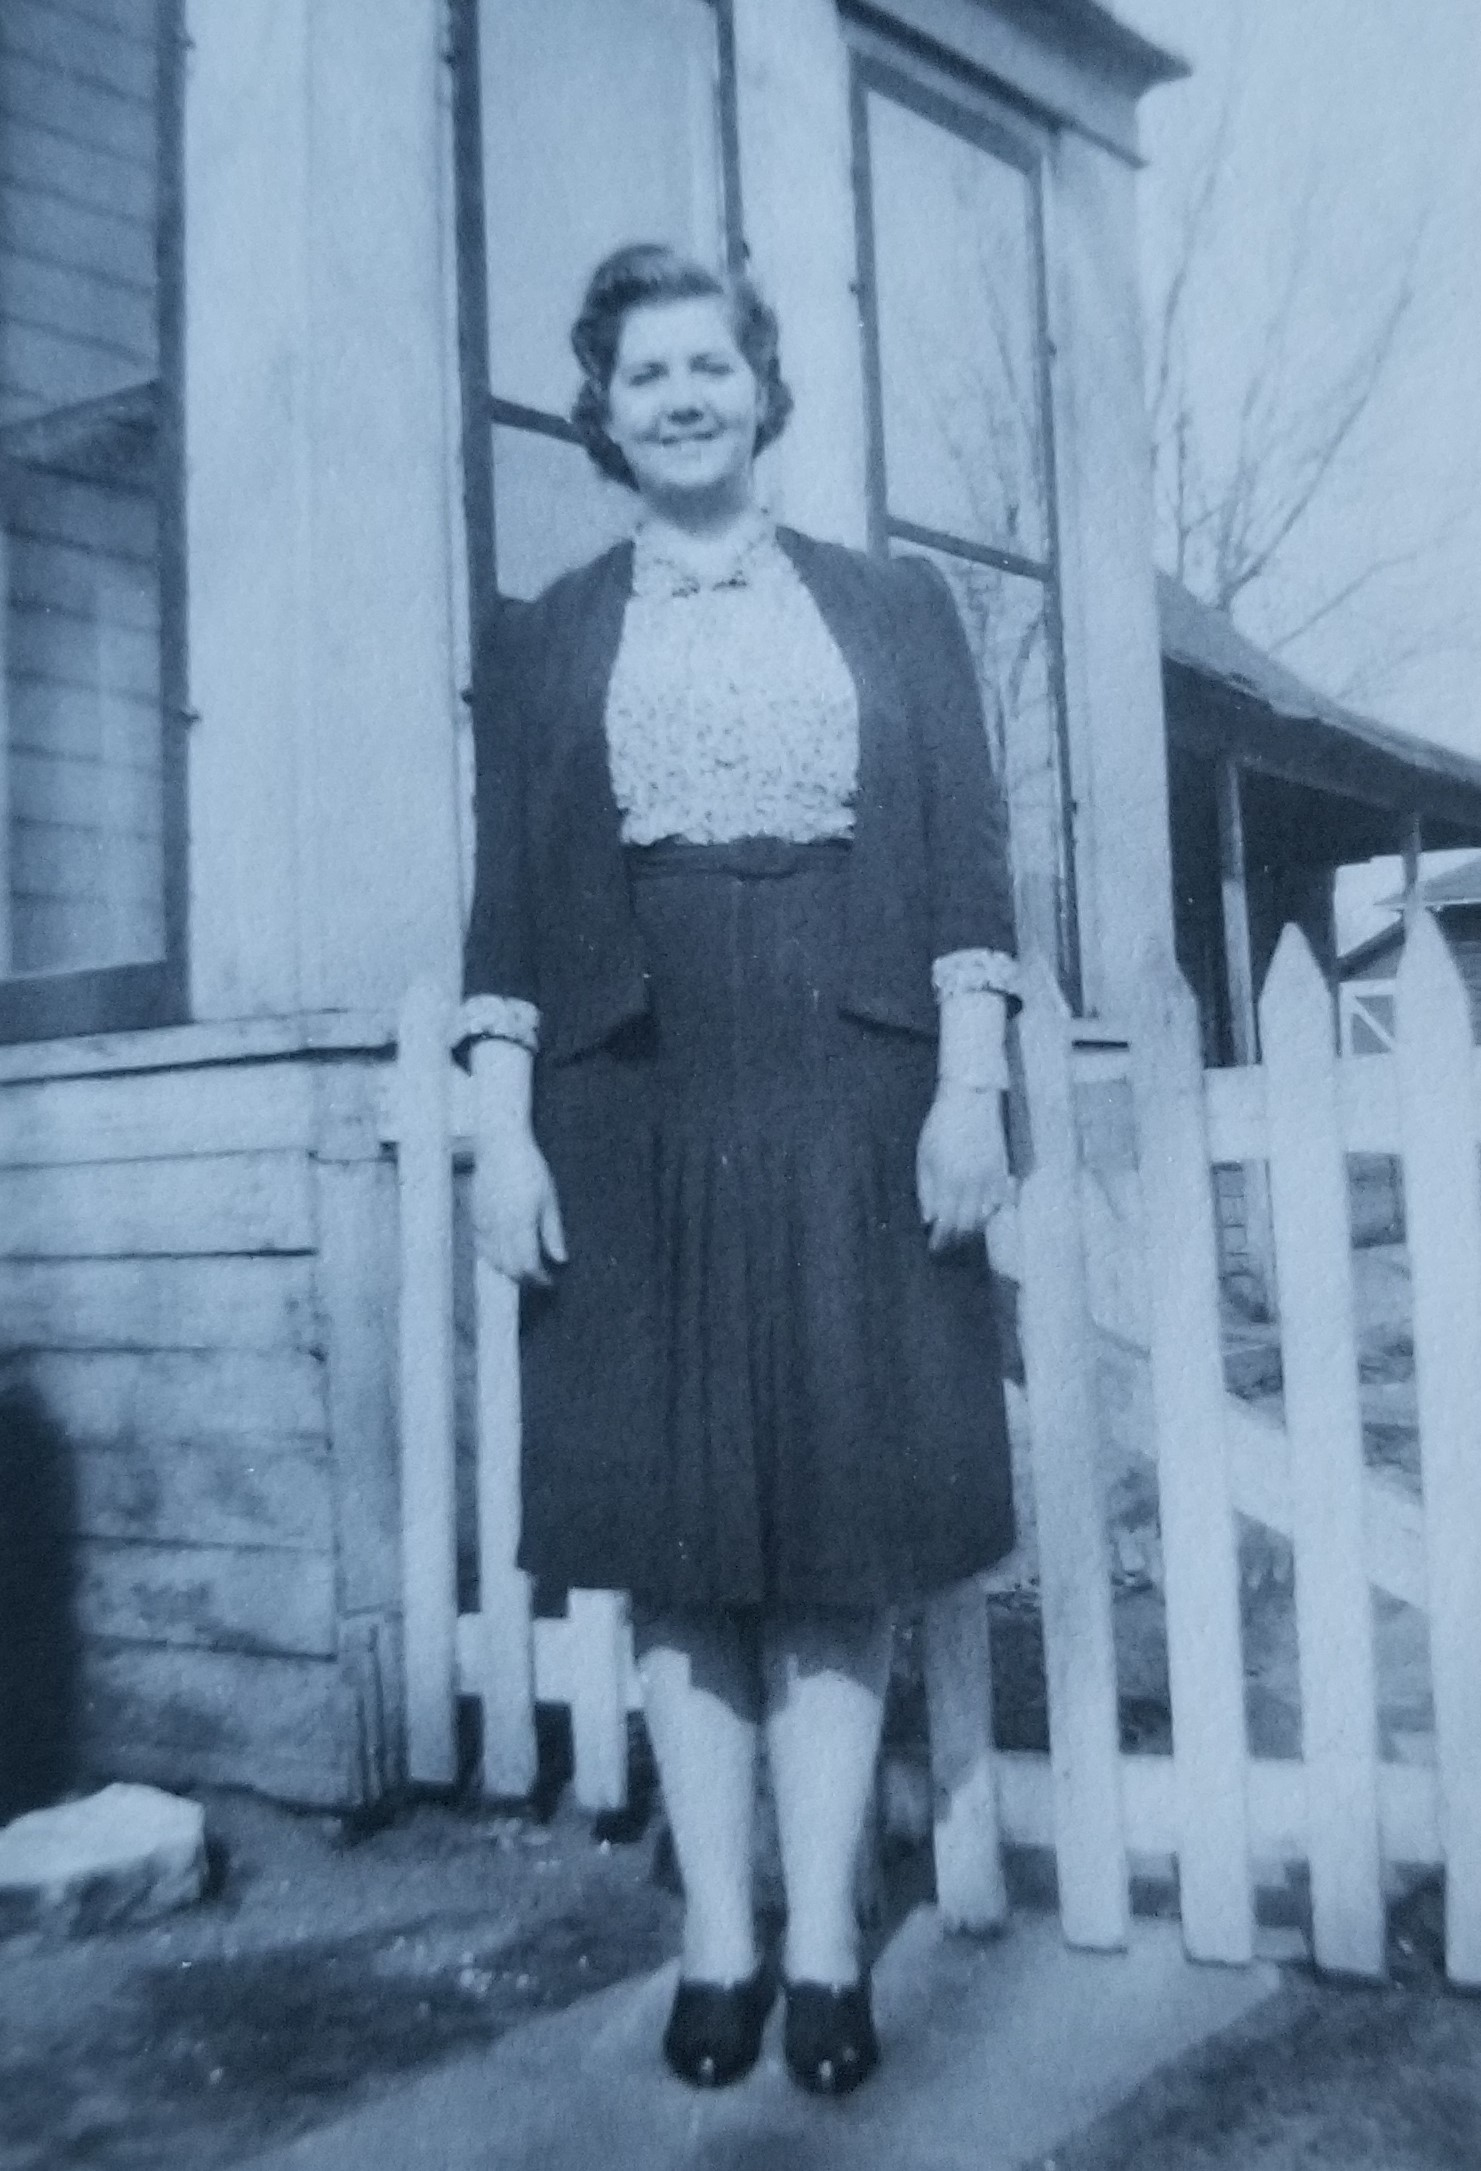
\includegraphics[width=0.65\linewidth,height=\textheight,keepaspectratio]{images/Akou15.jpg}

}

\caption{Lila as a young working woman, circa 1943}

\end{figure}%

By the end of the first week, Lila regretted that she had not said no to
Veda. Although summer was just getting underway, it was hot, and the
mosquitoes were thick. It was fun to pick berries on a Saturday---the
Slabacks had done that many times to get berries for jam---but doing it
every day was backbreaking work. The strawberries were low to the
ground. It was killing her knees. The blueberries grew on higher bushes,
but they were so small. It took a lot of picking to fill a single
bucket. The berries ripened in stages; by the time they reached the end
of the field, it would be time to go back and pick the berries that had
just ripened. She was grateful when Mrs.~Stanton asked if she would help
with cleaning and food preparation in the afternoon. Anything to get out
of the fields a little early.

Looy, Jean, and Patty were sleeping in the barn. Lila knew that Veda
would not approve of the ``mixed company,'' but her only choice was to
keep her private room or sleep in the barn with them. Lila decided to
keep the room. What Veda didn't know wouldn't hurt her. Besides---after
spending all day in the fields, what trouble could Looy and the girls
possibly get into? Lila was worn out from the work and assumed they were
too.

Four weeks later, the berry season was over. Mr.~Stanton thanked them
for their hard work and paid them each fifty dollars. Looy and the girls
were thrilled. All the way home, they talked about how they would spend
the money. Jean and Patty were giving part of their wages to their
parents, but Veda had already promised Looy that he could keep whatever
he earned. Lila was disappointed. She could have made more money in one
week by working at Carroll's.

A few months later, they heard that Jean was pregnant. Her parents had
decided that Looy and Jean were ``too young'' to get married, so they
sent her to live in a house for unwed mothers. It was supposed to be a
secret, but of course, everyone in the church knew. It was a major
scandal. A few days after they heard the news, Veda cornered Lila in the
kitchen and demanded to know why Lila had ``allowed'' this to happen
while they were on the farm. ``You were the adult! You were supposed to
make sure that nothing happened!''

Lila flushed with anger and frustration that Veda was blaming her. She
yelled, ``You and I were both there when Red asked Looy if he wanted to
be a man. What did you think was going to happen, Veda? Was I supposed
to treat him like a child?'' Sometimes while walking to and from work,
Lila wondered if Jean's baby would be a boy or a girl. Would he or she
be funny or serious? Would the baby grow up to be a factory worker or
maybe something more exciting like a famous wrestler? How could Jean's
parents force her to give the child up for adoption? How could Jean just
allow it to happen? Maybe Looy and Jean were too young to get married,
but it was a tragedy for everyone. The baby would never know that he or
she was a Slaback.

\section{Notes}\label{notes-29}

The work of cocktail waitressing combines food and beverage service with
adult entertainment. I know for a fact that Lila worked in bars as an
adult. She might have found the work exciting, but it was not very
socially acceptable. It's a very different lifestyle from being a
Catholic stay-at-home mother. Lila and Veda were naturally growing
apart. I imagine how difficult it would have been for Lila to be
confronted and judged by her not-much-older sister.

I stumbled across a tiny snippet of news that Lila and ``Loy'' were
picking berries in Minnesota in 1942. I questioned whether that was
Lloyd or Loyal, but I eventually realized that Lloyd was in prison
during that time. In this chapter, the job becomes a pretext for Veda to
get Lila out of her job and into something more wholesome. However, it
backfires on both of them when Lila fails to supervise Looy and one of
the girls (Looy's eventually wife in real life) gets pregnant. I have no
idea if they really had an unplanned pregnancy, but this story gives us
insight into two things:

\begin{itemize}
\tightlist
\item
  the pressure on girls and young women to avoid having a child out of
  wedlock, and
\item
  Lila's perspective on pregnancy and motherhood.
\end{itemize}

She is not eager to become a mother, but she is also sad (maybe even a
bit angry) that Jean has been forced to give away her child.

For more information, see Ylva Baeckström\footnote{\citeproc{ref-baeckstruxf6m2022a}{\emph{Gender
  and Finance: Addressing Inequality in the Financial Services Industry}
  (London: Taylor \& Francis, 2022)}.}, Stephanie Lynn Budin\footnote{\citeproc{ref-budin2021a}{\emph{Freewomen,
  Patriarchal Authority, and the Accusation of Prostitution} (London:
  Taylor \& Francis, 2021)}.}, and John C. Spurlock\footnote{\citeproc{ref-spurlock2015a}{\emph{Youth
  and Sexuality in the Twentieth-Century United States} (London: Taylor
  \& Francis, 2015)}.}.

\bookmarksetup{startatroot}

\chapter{Chapter Twenty-Nine}\label{chapter-twenty-nine}

The manager at Carroll's was thrilled when Lila returned and announced
that she was available to work again. Two of the waitresses had decided
to join the WAVES\footnote{The WAVES (Women Accepted for Volunteer
  Emergency Service) was a program established in 1942 that allowed
  women with a high school diploma to enlist in the US Navy. Since Lila
  had not graduated from high school, she was not eligible to join.},
and they had been short-staffed. In very little time, Lila was back to
her usual routine. There was no end in sight to the stream of soldiers
moving through La Crosse. Lila had stopped trying to remember the names
of her customers; even the ``regulars'' would be gone after a few weeks.

The price for a movie was reduced on Tuesday evenings; one week Lila
asked Myrtle if she would like to go. (``My treat,'' she said when
Myrtle objected to the cost). They decided to watch the latest movie
with Claudette Colbert, \emph{So Proudly We Hail!} Lila assumed that it
would be another comedy, but it was not. It was about women serving in
the army as nurses and falling in love with the soldiers. Myrtle cried
when one of the nurses was killed and said that the movie was ``so
romantic.'' On the way home she said that Carl was stationed in
California; she wanted to take the train and go visit him, but women
weren't allowed on the base. Lila wondered if that was the truth or if
Carl had reasons for wanting Myrtle to stay home in Wisconsin. Working
at Carroll's, she had observed that there was little difference in
behavior between the soldiers who were married and those who were not.
She wondered if she should tell Myrtle that she was being naïve but
decided against it. She didn't want to hurt her feelings.

The soldiers mostly went to the bars in groups. Every weekend, the city
of La Crosse was like a giant party. They played darts and card games,
smoked and drank, told jokes, and bragged about their exploits. One of
the waitresses, a tall, glamorous blonde, openly relished having sex
with them. Lila had never known a woman who was so open about it; she
was like a movie star. Claire received more tips than anyone, but then
one day she simply disappeared. Where had she gone? When Lila asked the
manager, he brusquely told her, ``Don't ask questions.''

Lila tried to memorize some of the jokes to share with Lloyd. One night,
she noticed a soldier who was sitting by himself in the corner. He was
older than usual and seemed to be lost in thought. When he nursed a
single beer for more than two hours, Lila took him a fresh one and said,
``There's plenty more where that came from.''

He smiled a bit and said, ``Thanks\ldots I don't know what I'm doing
here.''

Lila had met plenty of soldiers who were homesick or nervous or just
plain scared (not that they wanted to admit it), but this one\ldots it
was like he had come to the bar from a funeral. ``You mean, you don't
know why you came to Carroll's?'' she said.

The man chuckled. ``No, I know why I came to this bar\ldots I just don't
know what I'm doing so far from California, getting ready to head off to
war. This is not how I imagined my life would turn out.''

Lila sat down beside him; it couldn't hurt to give him a little extra
attention. He had sandy hair and smelled like cigarettes and Old Spice.

He started telling a story. ``A few nights ago, it was time for lights
out and the sergeant said, `Men, I want you to look up into the sky and
tell me what you see.'

One person spoke up right away and said, `Sir, I see millions of stars.'

The sergeant replied, `Alright. Now what do the stars tell you?'

Someone on the other side of the room said, `They tell me that I can
always find my way home as long as I look for the north star.'

Another said, `They tell me that God exists and everything else is
insignificant.'

My bunkmate added, `The stars tell me that the sky is clear tonight, and
the weather will be good tomorrow.'

It was a very somber mood. Then the sergeant barked, `You're all wrong.
If you can see the stars when you're in bed, then somebody stole your
damn tent.'\,''

Lila laughed out loud. He had told the joke with such a dry sense of
humor; Lila didn't think it was a joke until the punchline. ``You really
got me there. My name is Lila, by the way.''

The man smiled and held out his hand, ``Private Daniel Oxnard.''

A feeling like electricity rippled through her body when they touched.
Lila said, ``Well, I need to go back to work now, Daniel, but I'll bring
you another drink. Compliments of the house.''

Daniel stayed for most of the night, but he slipped out before they had
another chance to talk. It was a busy night and Lila had made over
fifteen dollars in tips. Before leaving work, she slipped the
five-dollar bills into her brassiere. (One of the other waitresses had
told her, ``A thief might take your purse, but the money will be safe if
you keep it close.'') By the time she returned to the neighborhood, the
sun was peeking over the horizon. A few nights later, Daniel was back.
As soon as she noticed him, Lila made a beeline for his table. ``Welcome
back, soldier. I wasn't expecting to see you again.''

Daniel replied, ``Well, a bad penny always turns back up.''

Lila laughed, ``I wouldn't say you're a bad penny. I'm glad you came
back.''

He sat in the corner again and ordered a beer, but when Lila brought the
drink to his table, he asked when her shift would be done.

``3:00,'' she said, thinking how long it had been since someone offered
to walk her home. Her shift flew by. She found Daniel standing in the
parking lot, waiting and smoking a cigarette.

He smiled and said, ``Where to?''

Carroll's was on French Island. There were many islands in the
Mississippi, but this was the largest one in the area. Lila smiled back
and said, ``This way,'' pointing in the direction of the Clinton Street
bridge.

That day the weather was unusually warm for September. The cicadas were
buzzing; it felt more like summer than fall. After they crossed the
bridge, Daniel asked, ``Can we walk by the river for a little while?
I've never seen the Mississippi up close before. I feel like I'm in a
Mark Twain novel.''

``Sure,'' said Lila. It was no special thrill for her to see the river,
but she didn't mind taking a detour. When they got to the shoreline, she
took off her shoes and put them in her handbag; it would be impossible
to walk along the sand in heels.

The moon was full that night, and the air was thick with humidity.
Daniel said, ``I was a truck driver back home\ldots my family is in the
sugar business.''

``Oh?'' said Lila. ``My oldest brother is a truck driver too. My family
is in the plastering business.''

``Plastering like\ldots the walls? Or getting plastered?''

Lila laughed, ``A little of both, I guess.'' How had he guessed about
the drinking problems in her family? It was like he could read her mind.

Soberly, Daniel said, ``I'm a tank driver now. We got our marching
orders this week; we're heading to Europe in a few days.''

Lila put her hand on his bicep. ``I don't know what to say, but I hope
you make it back.''

Daniel put his hands on her waist. ``I want to make love to you Lila.
You're so beautiful and I miss being with a woman.'' His hands were warm
and gentle. It had been over a year since Lloyd was arrested. She leaned
over and kissed Daniel. He untied the front of her dress, and they sank
down into the sand. It was like being in a movie. Lila wanted to give
him a happy memory; one last enjoyment before going off to war. It was
so passionate and romantic. They could have been spotted by anyone
passing by, but Lila did not care.

\section{Notes}\label{notes-30}

The last chapter of Part I is extremely fateful: Lila meets a funny,
handsome soldier. He asks to walk her home (something Lloyd often did)
and she accepts. Although she knows that not all soldiers are
trustworthy, movies have primed her for the thrill of spontaneous
``romance,'' like having sex on a moonlit beach with a soldier who is
heading off to war.

The timeline is accurate for the conception of Lila's first real-life
child, Myrtle.

For more information, see Evan Bachner\footnote{\citeproc{ref-bachner2008a}{\emph{Making
  WAVES: Navy Women of World War II} (New York: Harry N. Abrams, 2008)}.},
Kathrina Glitre\footnote{\citeproc{ref-glitre2013a}{\emph{Hollywood
  Romantic Comedy: States of Union, 1934--1965} (Manchester University
  Press, 2013)}.}, and Larry King\footnote{\citeproc{ref-king2001a}{\emph{Love
  Stories of World War II} (New York: Crown Publishing, 2001)}.}.

\bookmarksetup{startatroot}

\chapter{Part II: In a Family Way}\label{part-ii-in-a-family-way}

\begin{figure}[H]

{\centering 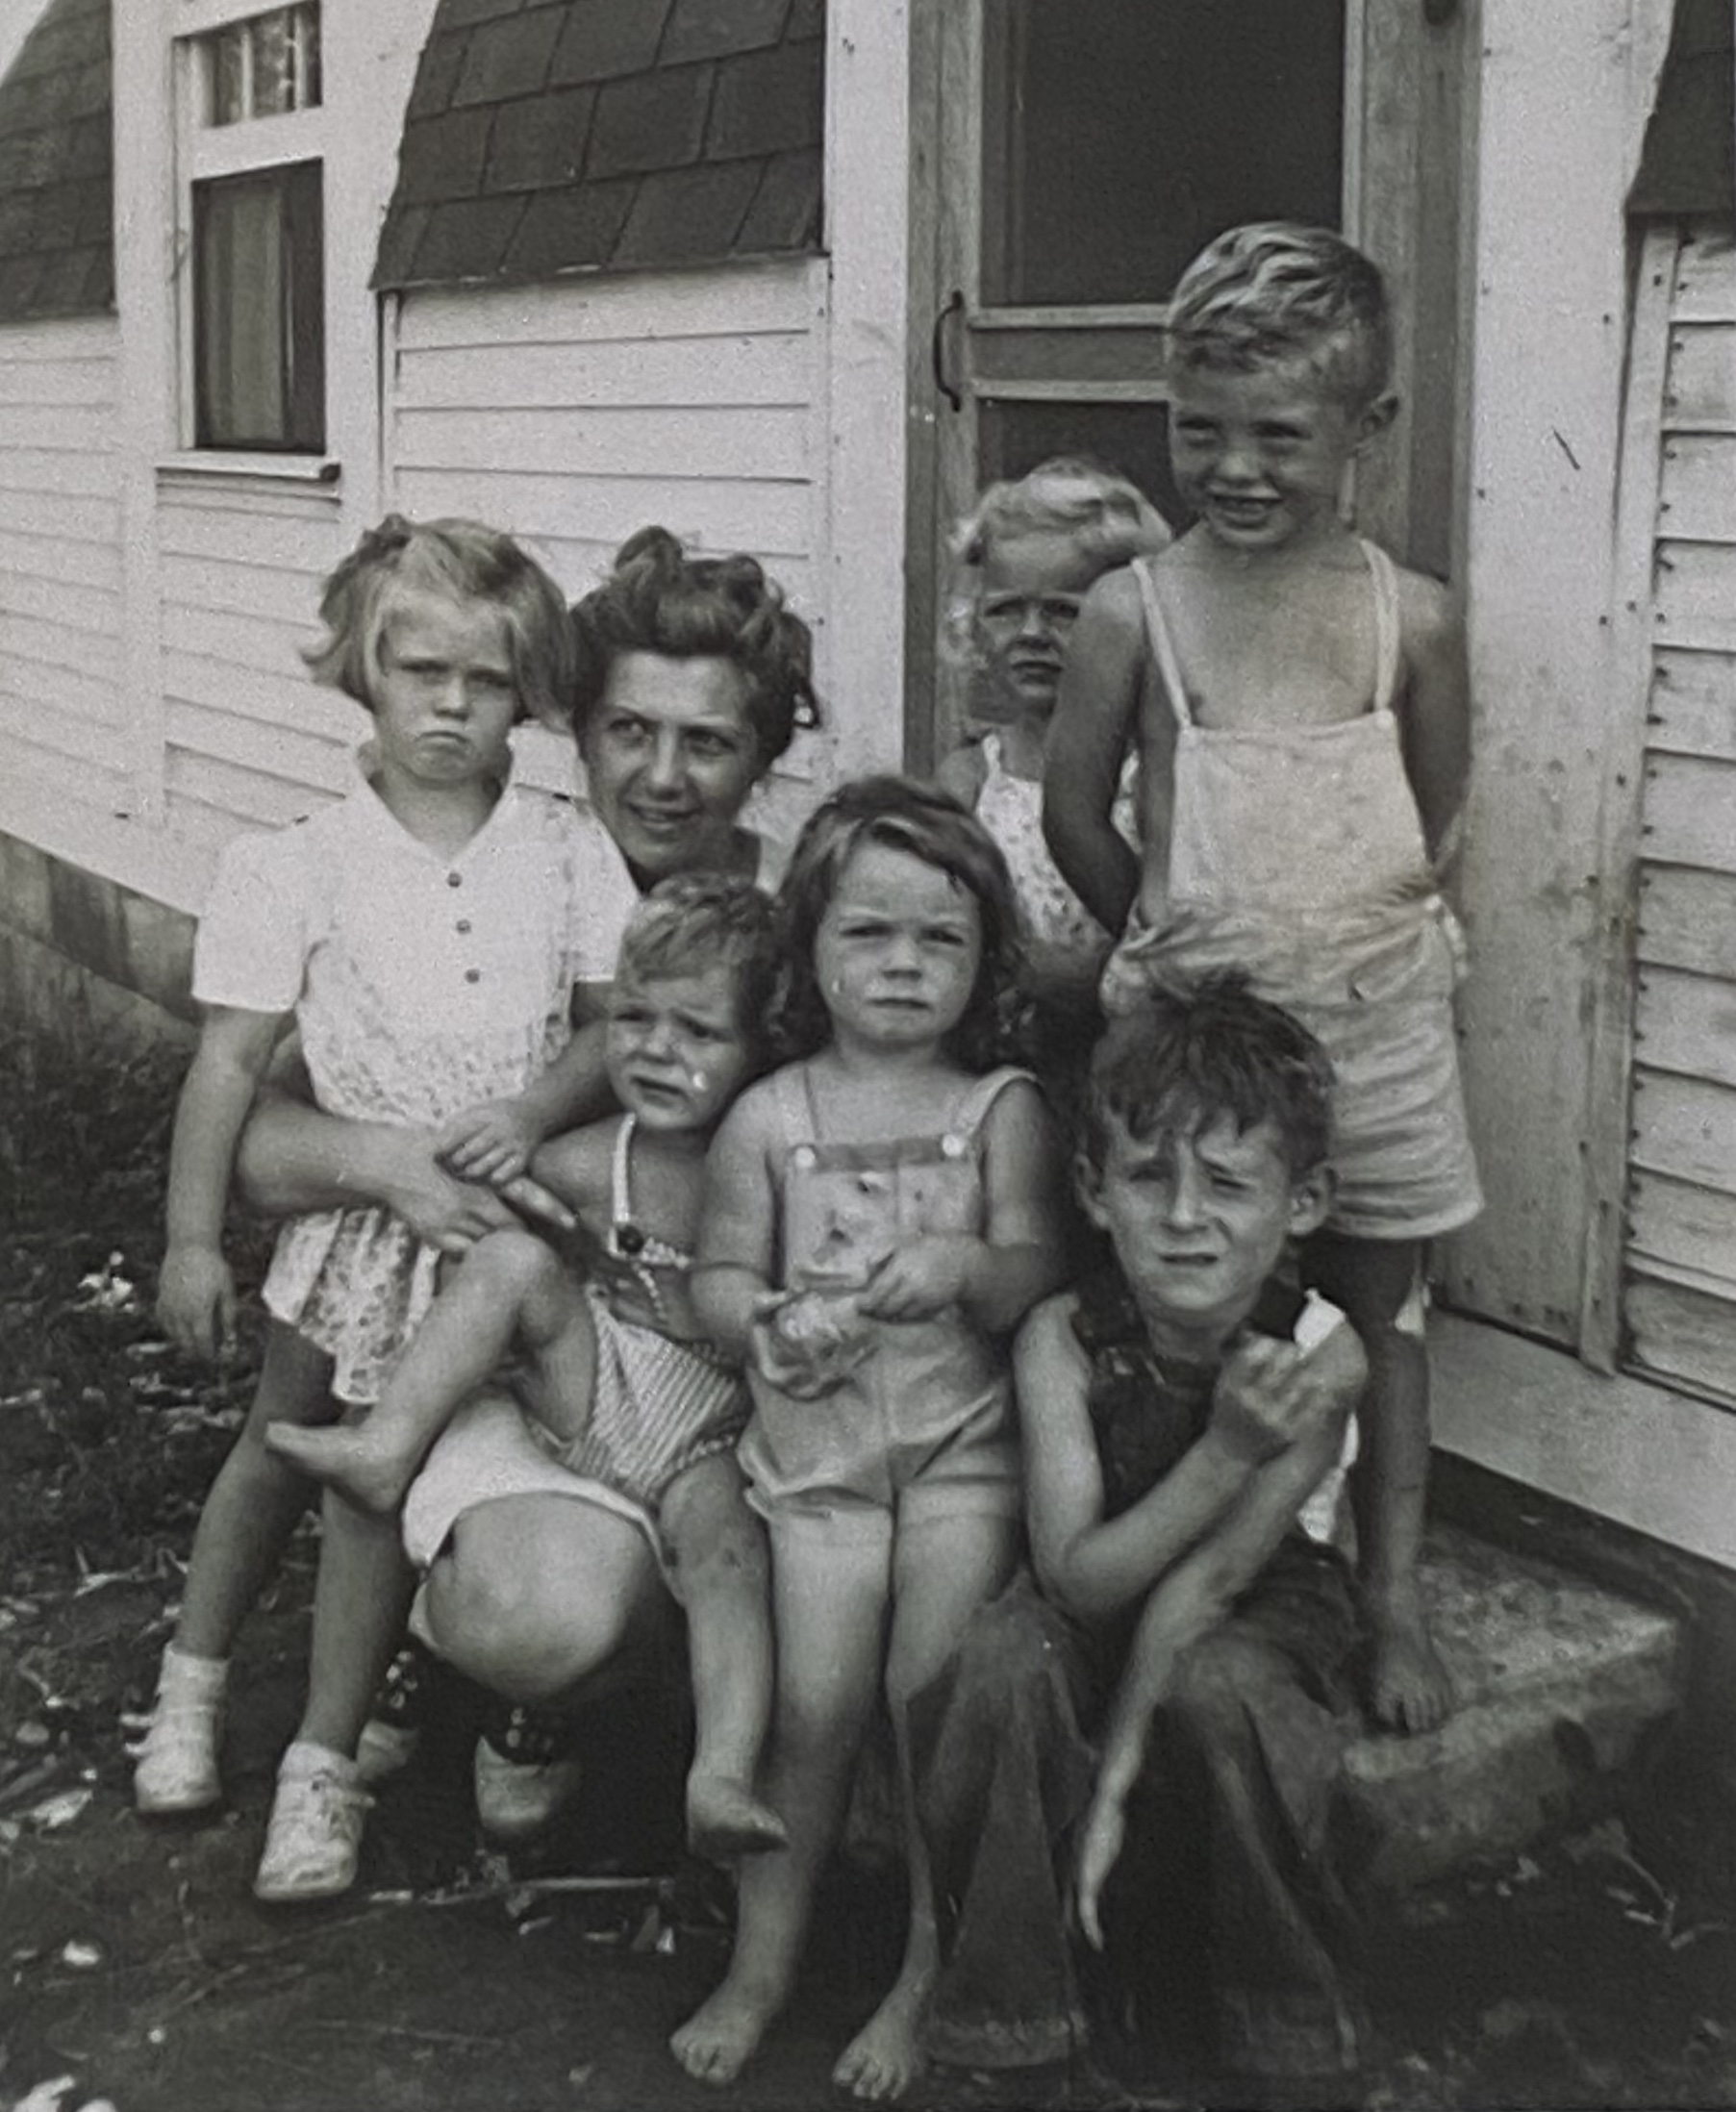
\includegraphics[width=0.75\linewidth,height=\textheight,keepaspectratio]{images/Akou16.JPG}

}

\caption[Lila, circa 1948.]{Lila, circa 1948. In the center is her
oldest daughter, Myrtle Joyce. Her son, John, is sitting in her lap.
Standing on her left are Veda's children, Patty and David.}

\end{figure}%%
\begin{figure}[H]

{\centering 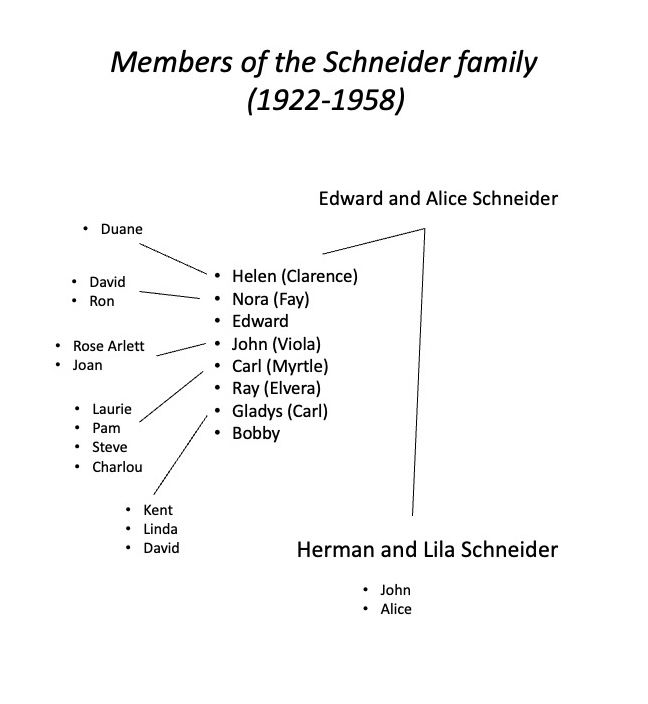
\includegraphics[width=0.85\linewidth,height=\textheight,keepaspectratio]{images/Akou17.jpeg}

}

\caption[Members of the Schneider Family 1922--1958]{I developed this
genealogical chart using data from
\href{https://www.ancestry.com/}{ancestry.com}. It does not include most
of Lila's children, because Herman only fathered her second and third
children (John and Alice). Alice was my mother.}

\end{figure}%

\section{Notes}\label{notes-31}

In this part of the book, we are introduced to the Schneider family of
West Salem, which Viola and Myrtle Johnson have already married into.

\bookmarksetup{startatroot}

\chapter{Chapter Thirty}\label{chapter-thirty}

Within two weeks, Lila knew something was different. Her first clue was
that her clothes suddenly felt like sandpaper on her skin. One evening
during her shift at the bar, she felt sick to her stomach and had to
excuse herself for some fresh air. Maybe it was food poisoning. On the
way to work, she had been so hungry that she stopped at White Castle to
purchase a hamburger. She kicked herself for stopping there when she
could have eaten as much food as she wanted at Carroll's. What was she
thinking? A few weeks later, she realized that her time of the month had
not happened yet. She tried not to think about it. Lila was hungry all
the time, especially for beef, baked potatoes, and ice cream. Her
uniform was getting tight, and she thought (regretfully) that she would
have to stop eating so much. For a little while, she was successful at
eating less, but around Christmas, she realized that it was no use; she
would have to buy a larger uniform after the holidays. If Veda noticed,
she didn't say anything.

One night at the end of January, Lila fainted at work. She had been
feeling a little sick but didn't want to admit it. Carroll's was always
busy. If she took time off, she would have to find someone to cover her
shift; the manager wouldn't like it. He was even less thrilled when Lila
fainted, but he drove her to the hospital. She woke up hours later in a
bed at St.~Francis. A nurse had been sitting in the room; as soon as
Lila opened her eyes, she left to fetch the doctor. Dr.~Olson was a tall
man with dark hair, horn-rimmed glasses, and a severe expression. His
stout belly stuck out from his white jacket, which was open in the
front. He sat down next to the bed and said, ``Do you know why you're
here, Miss Slaback?''

Lila had never been in the hospital before. She felt very tired and
silently shook her head.

The doctor looked down at his clipboard and said, ``Miss Slaback, are
you engaged or married?''

This again. Why did everyone care so much?

When she didn't answer, he said, ``Do you have a family member that we
can call? Someone will need to pick you up later today.''

Her head was swimming. It was like being in a dream; she could hear the
doctor speaking, but nothing was making sense. She managed to give him
Veda's name and address before she fell asleep again.

\begin{figure}[H]

{\centering \pandocbounded{\includegraphics[keepaspectratio]{images/Akou18.jpg}}

}

\caption[A postcard of St.~Francis Hospital from the 1920s]{A postcard
of St.~Francis Hospital from the 1920s; it was the first major hospital
in La Crosse, established by the Catholic Church in 1883.}

\end{figure}%

When she woke up the next time, Veda was sitting next to her. She looked
so worried that Lila immediately felt terrible. Veda said,
``Lila\ldots the doctor says you're pregnant.'' Her words were like a
lasso that jerked her consciousness back to the surface.

``I don't understand. What are you doing here?'' She sensed that Veda
was angry.

``I'm here because someone came to our house and informed me that you
were taken to the hospital.''

Lila responded, ``I'm sorry, I didn't mean to cause you any trouble. I
don't understand what's going on.'' Lila ran her fingers over the white
sheets of the hospital bed. The sheets were cool and stiff.

Veda's eyes narrowed. ``The reason you're at the hospital, Lila, is
because you're pregnant. You're anemic from a lack of iron and that's
the reason why you fainted.''

``Oh,'' said Lila.

They sat together in silence until the nurse returned to give Lila an
injection.

Veda had left her son with a neighbor before rushing to the hospital.
Red picked them up as soon as he was done with work. He gave Veda a kiss
on the cheek, and she pulled him off to the side for a hushed
conversation. When Lila had checked out from the hospital, the nurse
gave her instructions to eat liver at least twice per week and to get
some rest. Lila hated liver; it tasted like meat, but the texture was
like peanut butter. It made her gag to think about eating it. She was
thinking about it when Red and Veda returned to the truck. Red opened
the door for Lila without saying a word. The ride back to Kane Street
was completely silent.

For the next two days, Lila slept. She had rambling dreams about car
accidents and about being chased. Her legs were so heavy that she
couldn't run away from whatever was chasing her, but she was never able
to see what the ``thing'' was. In one dream it was chasing her along a
cliff, and she fell off the edge. It jolted her awake with her heart
racing. Someone had placed a chair next to the bed. It was holding a
glass of water and a sandwich on a plate. She reached out and touched
the top of the bread, but it was stale. Too tired to complain or to make
something fresh, she forced down the sandwich, which turned out to be
peanut butter. The water wasn't enough to wash away the dryness. She
fell asleep thinking how thirsty she was.

On the third morning, Lila was violently awakened by a splash of
ice-cold water. Her mother was standing near the window holding a
bucket. ``You good-for-nothing whore,'' she snapped. ``I thought I
raised you better than this.'' Lila was shocked. It felt like her heart
had stopped beating for a few seconds. ``Well, what do you have to say
for yourself? I'm waiting here until you answer.''

Was there anything she could say to make this go away? ``I'm sorry,''
Lila stammered. ``I don't know what you want me to say.''

Hazel was so enraged that her face was nearly purple. She threw the
bucket against the wall, and it fell to the floor. Clang-clang. She
stomped to the door and slammed it behind her. Lila decided to dry
herself off and to get dressed. She needed to use the bathroom and was
feeling very hungry and thirsty. As soon as she left the bedroom, she
noticed that Veda and Red, her parents, and Aunt Hattie were all sitting
around the dining room table---like cats getting ready to pounce on a
bird.

With an innocent tone, Lila said, ``I need to use the bathroom; be right
back.''

Aunt Hattie hissed, ``Be quick about it, we're all waiting for you.''

Lila looked at herself in the mirror. Her eyelids were puffy, and her
hair was a mess. The back of her nightgown was soaked. Her thoughts
flashed back to the hospital and Veda saying, ``You're pregnant, Lila.''
She closed her eyes and wished that she could be magically transported
somewhere else---like Dorothy in \emph{The Wizard of Oz}. She stood at
the sink and clicked her heels together, but when she opened her eyes,
everything was exactly the same.

After changing her clothes and combing her hair as slowly as possible,
Lila went to the table and sat down. The table was covered with crumbs
and plates and half-empty cups of coffee. She reached out for a piece of
bread, and Aunt Hattie cleared her throat. ``Lila\ldots you should be
ashamed of yourself. Your actions have brought disgrace to this entire
family.'' Lila pulled her hand back and looked down at the table. Hattie
continued. ``Who is the father of this child? I assume it's Earl
Bright?''

Veda said, ``Earl married someone else. He wrote a letter to Lila and
told her.''

Hazel snorted. ``I knew it.''

(Later, Lila wondered why Veda had not told anyone.)

``Well,'' Aunt Hattie demanded, ``Who is the father then?''

Lila was silent. She thought about that night by the river with Daniel
and wondered if he was still alive. They had not written letters to one
another; he had no idea that she was pregnant.

Everyone was staring at her. She resolved that she would not give them
the satisfaction of watching her cry. After what felt like an hour, Aunt
Hattie said, ``You have two choices: you can either get married, or you
can give the baby up for adoption.'' Lila looked around the table. Veda
was as white as a ghost and looked like she wanted to sink under the
table. Hazel's face was beet red and there were veins standing out on
her neck that Lila had never noticed before. Her father and Red were
staring into their cups of coffee. Aunt Hattie's lips were tightly
pinched, and she was waiting for an answer---she was staring right at
Lila without blinking. Her mother spoke up and said, ``She should go to
that home for unwed mothers\ldots the one that Jean's parents sent her
to.''

Aunt Hattie said sharply, ``That is certainly one option, unless the
father in planning to step forward and make Lila an honest woman.''

An honest woman? It was terrifying to feel so angry and ashamed, worse
than anything Lila had experienced before. When she finally managed to
speak, her response surprised her: ``I guess I'll be getting married
then, because I am not a child, and I am not giving this baby away.''
She was not sure if that was true, but the words just poured out of her.

Hazel stood up and said, ``I want to leave now. I'm going to Cecil's
house.''

Veda started to cry.

\section{Notes}\label{notes-32}

This chapter is largely drawn from my own experiences as a newly
pregnant mother (although I was married at the time, and it was an
intentional choice, not a scandal.)

Shaming is a destructive form of emotional abuse that often occurs
within families. As a not-very-happy child, I often imagined that I was
Dorothy from \emph{The Wizard of Oz}. If I clicked my heels together and
concentrated hard enough, maybe I would open my eyes and discover that I
was somewhere else. The imagery of the hospital and nursing staff is
based on my research on the history of work uniforms (including medical
uniforms).

For more information, see David G. Hogan\footnote{\citeproc{ref-hogan1999a}{\emph{Selling
  'Em by the Sack: White Castle and the Creation of American Food} (New
  York University Press, 1999)}.}, Carin Modh, Ingela Lundgren, and
Ingegerd Bergbom\footnote{\citeproc{ref-modh2011a}{{``First Time
  Pregnant Women's Experiences in Early Pregnancy,''}
  \emph{International Journal of Qualitative Studies in Health and
  Well-Being} 6, no. 2 (2011),
  \url{https://doi.org/10.3402/qhw.v6i2.5600}}.}, and June Price Tangney
and Ronda L. Dearing\footnote{\citeproc{ref-tangney2002a}{\emph{Shame
  and Guilt} (New York: Guilford Publications, 2002)}.}.

\bookmarksetup{startatroot}

\chapter{Chapter Thirty-One}\label{chapter-thirty-one}

That afternoon when the house was quiet again, Veda told Lila that she
would have to stop working. What if she fainted again? It wasn't safe
for her or the baby. She said it with a gentleness that had been absent
from the conversation with Aunt Hattie and their mother. Lila wanted to
push back and tell her to mind her own business, but Veda had a point.
She would have to take better care of herself if she was going to keep
this baby. She had never thought much about becoming a mother, but she
was beginning to feel a deep longing for the child growing inside of
her. A child of her own: nobody was going to make her give it up.

For the rest of the month, Lila mostly kept to herself. After a few
awkward dinners, she decided to eat alone in her room; it was better
than facing the look of rejection on Red's face. She missed going to
work though. She missed earning money and flirting with men at the bar.
She missed hearing their jokes and laughter. Most of all, she missed
leaving the house. There was a cloud of shame hanging over all of them.
Lila couldn't go to church in her ``condition.'' Going outside for any
reason was risky; the neighbors were sure to notice.

One cloudy day in February, Lila decided that she needed some fresh air.
She slipped out of the house while Veda was shopping for groceries. She
didn't have any destination in mind. It was just good to be outside.
After walking for a few blocks, she decided to head in the direction of
Myrtle's house. When she rang the doorbell, Myrtle answered right away
and invited her in for cookies and tea. It was such a relief to see a
friendly face. Myrtle didn't know anything yet about the pregnancy. It
was warm and cozy inside. Myrtle was barefoot and wearing a house dress
and a white apron; she was in the middle of making a coffee cake for a
luncheon at the church. ``Take your coat off and stay a while,'' she
said.

When Myrtle turned her back to check on the cake, Lila took off her coat
and hung it in the little closet by the front door. By the time Myrtle
had turned back around, Lila was sitting at the table. ``I haven't seen
you in ages!'' she said gleefully. ``I have so much news to tell you.''
Her sister, Viola, had given birth to a baby girl in November, her
parents' second grandchild. Myrtle had crocheted a blanket for the
christening and was making her a layette. There was a tiny sweater lying
on the sofa. As Myrtle rattled on about Viola's two precious little
girls, Lila thought about her own impending ``miracle.'' The hot tea was
making her feel a bit dizzy.

After an hour Lila said, ``Thanks for the tea; I guess I should be
going.''

Myrtle replied, ``Why don't you stay for dinner? If you don't, I'll just
end up eating cheese and crackers and reading a trashy romance until
midnight. You have to save me.'' They both laughed.

``I guess I could,'' said Lila.

``Great! I'll get some sausages from downstairs, and you can peel the
potatoes. They're in the cabinet near the door.''

Feeling relaxed, Lila got up to look for a paring knife. She could hear
Myrtle coming back up the stairs. She flipped the switch at the top of
the stairs and said, ``These sausages are really good.''

Lila was standing at the sink washing the potatoes when Myrtle put her
hand on her shoulder. With a tone of astonishment, she said,
``Lila\ldots are you\ldots pregnant?'' Lila didn't answer, so Myrtle
continued. ``Why didn't you say anything? Who is the father?'' A tear
rolled down Lila's cheek, and Myrtle gave her a hug. ``I'm so sorry that
I didn't notice before. Bring a chair from the table and I'll peel the
potatoes.''

As they made dinner, Lila told her about Daniel. It felt good to talk.
Being with Daniel that night had been a moment of beautiful pleasure,
except---now here she was, pregnant and unmarried. Myrtle usually did
most of the talking, but this time she was quiet. By the time Lila
finished telling the story (including how her family had reacted),
Myrtle was at the stove frying the sausages and hash browns. She said,
``You're really in a pickle, Lila. What are you planning to do now?'' It
was a question and not a demand.

``I told them I would get married and keep the baby, but I don't know
how to pull it off. How can I find a man who will marry me like this?''

As they ate dinner Myrtle said, ``I have an idea. Carl has an older
brother who never got married. His name is Herman, and he works as a
hired man on a farm. He's shy, but he's nice.''

Lila said, ``A farmer? No thanks.''

Myrtle swallowed her bite of sausage and said, ``Beggars can't be
choosers. You should at least give Herman a chance. I'm going out to
West Salem next weekend for lunch with the Schneider family. Herman will
be there, and you can go with me as my friend. Maybe it will turn out to
be nothing, but it will get you out of the house. Viola and her husband
John are picking me up. I'm sure they won't mind if we pick you up
too.''

As they said their goodbyes with another hug, Lila promised that she
would go with them.

\section{Notes}\label{notes-33}

In this chapter, we learn more about the changing relationship between
Lila and her older sister, Veda. Veda cares about Lila, but she fears
rejection from her family, her church, and her own husband---her
compassion can only extend so far. The acceptance Lila receives from
Myrtle contrasts sharply with the behavior of the Slabacks.

Until the ``baby boom'' started after World War II, pregnant women were
generally expected to conceal their condition (e.g., with a maternity
corset) or stay home. As an unmarried woman, the pressure on Lila would
have been especially intense. Page Boy, the first ready-to-wear
maternity clothing brand in the US, had only just begun selling their
designs nationwide in 1939.

``Take your coat off and stay a while'' is a phrase I heard often
growing up. It's friendly but also a bit sarcastic, as if the visitor
doesn't have enough sense to shed their winter coat without being asked
to do so. The phrase, ``beggars can't be choosers,'' is also
passive-aggressive.

For more information, see Kay Goldman\footnote{\citeproc{ref-goldman2013a}{\emph{Dressing
  Modern Maternity: The Frankfurt Sisters of Dallas and the Page Boy
  Label} (Lubbock: Texas Tech University Press, 2013)}.} and Pamela
Regis\footnote{\citeproc{ref-regis2013a}{\emph{A Natural History of the
  Romance Novel} (Philadelphia: University of Pennsylvania Press,
  2013)}.}.

\bookmarksetup{startatroot}

\chapter{Chapter Thirty-Two}\label{chapter-thirty-two}

Lila had not seen Viola since she dropped out of school to get married.
Myrtle was in the car with them, holding the baby in the back seat.
``Get in!'' she said. ``You can hold Joan.'' John was driving. He was
tall with dark hair and a ruddy complexion. Lila wondered if he looked
like his brother, Herman. She was feeling nervous about meeting him.

Earlier that week, Lila had gone shopping downtown. Her clothes were
getting so tight, but she had never been handy with a sewing machine.
Viola had purchased a new one and said that Lila could use it, but when
she sat in front of the machine her head was filled with echoes of her
mother's voice: ``You're going to break it! Don't do it that way. What
did I tell you?! You couldn't sew a straight line if your life depended
on it.'' She had the money from waitressing, so why not spend a little?
After combing through the racks at Woolworths for a while---wondering
what size dress she would need in her ``state'' and working up the
courage to try some things on---she stumbled into a small section of
maternity clothing. It didn't look that different from the rest of the
clothing on the floor, but when she tried on a dress, she realized that
it had extra buttons on the inside that would allow her to adjust the
size as her belly grew. She bought four dresses in a flattering wrap
style. The cotton fabric would be chilly for the rest of the winter, but
her skin was too sensitive for wool.

Her dress for the trip to West Salem was brown with tiny yellow and
orange daisies. It wasn't glamorous, but it was presentable. Lila had
giggled in the mirror that morning thinking about what a ``knocked-up
cocktail waitress in need of a husband'' would look like, but this
wasn't the day for truth-in-advertising. Her feet were starting to swell
and felt pinched inside her shoes. She had purchased a pair of brown
wool stockings---a concession to wholesomeness---and they were making
her legs itch. The only thing she was happy about was her hair. She
didn't love the color, but it was thick and shiny and beautifully
curled. She had pinned it back on one side with an elegant gold-colored
barrette. As Viola, Myrtle, and John chatted about the latest gossip
from West Salem, the baby fell asleep in Lila's arms. Her eyelashes were
so long and delicate, and she smelled heavenly. Her tiny fist was
wrapped tightly around Lila's finger.

The drive to West Salem did not take long. It was cold and sunny, and
the trees glittered like diamonds. The Schneiders lived in a tiny house
on the edge of town. The front stairs were crumbling, and the house was
overshadowed by an enormous pine tree. Gladys, John's younger sister,
was at the front door waiting to welcome them in. There was no turning
back now. The house smelled like naphtha soap and roast beef. John's
mother, Alice, gave Viola and Myrtle a hug, and then she turned and
said, ``Welcome; you must be Lila,'' with a slight German accent. She
was wearing a long dress and a beautiful shawl that she had knitted
herself using different shades of brown wool. She gave Lila a hug like
they had known one another for years. It made Lila feel better about
being there.

A few minutes later John's older sister, Nora, walked through the door
with a small boy. Her dress was shorter and more fashionable. She kissed
her mother on the cheek and put on an apron to help with the cooking.
Where was everyone else? Lila sat down at the table and looked around
the main living area. There wasn't much to see. There were two doors
leading to the bedrooms. A cast-iron stove provided heat and doubled as
an extra place to cook. On the wall next to the table was a calendar
from 1935 with a bouquet of flowers. It was the only colorful thing in
the room. There was no radio and---Lila realized with horror---no indoor
plumbing. She dreaded trudging through the snow and using the outhouse,
which was sure to be unheated.

As she listened to the family's chatter, she learned that John had
another older sister, Helen, who lived in La Crosse. Her husband had
died in a tragic hunting accident not long after their son was born. She
was raising him alone and worked in the Trane factory on the south side
of the city. (Lila had heard of it but was not familiar with any of the
neighborhoods south of downtown.) Nora's son, David, was the third
grandchild. Viola's children, Rose and Joan, were the second and fourth.
Alice clearly loved visiting with all of her grandchildren. Rose and
David took turns bouncing on her knees; they were gleeful as she
performed little rhymes that Lila did not understand. Gladys and Nora
were finishing up the meal. As they distributed the tin plates and
well-used silverware, Herman, his father Edward, and the youngest
brother, Bobby, arrived. They had been milking cows and smelled faintly
like hay and manure.

Herman washed his hands in a basin by the front door and sat across the
table from Lila. He was very quiet. They didn't speak to one another
during the meal. Lila wasn't sure that he even noticed her. He was very
tall and slim and ate his boiled carrots, salted potatoes, and slice of
roast beef in silence. His flannel shirt was heavily patched. He had
dirt under his fingernails and sad-looking eyes.

Nora asked Lila if she would like another cup of tea and said, ``Tell us
a little about your family, Lila. What are they like?''

Everyone stopped talking and turned their heads. Lila blushed. ``Well,
I'm not sure what to tell you.'' In her mind, she was thinking of her
life in the city---the streetcars, the bustle of people going about
their business, the movie theater where Veda had met Red, working at
Carroll's---it was different from West Salem, which was a much smaller
town. She didn't want to offend them or reveal too much about her
situation. After a few moments, she said, ``My parents used to be
farmers. We moved to La Crosse when I was five years old, so I don't
really remember it, although we sometimes went out into the country to
see relatives and pick apples. My parents recently left the city, so I'm
living with my sister. I have two sisters and five brothers;
well\ldots four brothers, since one of them died in a car accident.''

Myrtle blurted out, ``I didn't know that your parents were farmers.''
They had been friends for a while at that point, but Lila was not
surprised. Myrtle was not a very good listener. For the benefit of
everyone in the room, Myrtle cheerfully added, ``Lila and I went to
grade school and high school together.'' She beamed as Lila smiled
awkwardly.

After the meal, Nora suggested that they should go for a walk. Herman
joined them, but as they approached the stockyard by the railroad
tracks, he said, ``See you later\ldots I have some errands to run before
I head back to the farm.'' It was the only thing Lila heard him say that
afternoon.

Once he was gone, Gladys leaned in and said, ``Lila! You have to tell us
what it's really like to be in the city. There must be so many handsome
men there.''

For a second, Lila imagined what it would be like to have Gladys as a
sister-in-law. It was an appealing thought. Gladys was not married, and
they were close in age. ``You should come visit,'' said Lila. ``That
would be so much fun!''

Gladys replied, ``I've known all the men in this town since they were
little boys and I'm bored to death with them.''

The village of West Salem was only a few blocks wide and a few blocks
long. As they walked, Gladys pointed out Christ Lutheran (which the
family faithfully attended every Sunday morning), the creamery, the high
school, and the photography studio where Nora worked. There was one
block of shops along Leonard Avenue with a hardware store and a small
movie theater. When they returned, the children were sleeping, and the
house was very quiet. Viola said that she would stay there while John
drove Myrtle and Lila back home. Nora and Gladys gave everyone a hug. As
Lila was buttoning her coat, Alice said, ``I hope we will see you again,
dear.'' She put her hand on Lila's belly and smiled. Lila had said
nothing about the pregnancy or her reasons for visiting, but it was
clear that Alice understood.

\section{Notes}\label{notes-34}

My mother was brilliant at sewing but very impatient and critical when
teaching me. To this day, I prefer sewing by hand. I don't know if
Lila's experience was similar, but I used this chapter to draw in a
little research on the history of maternity clothing.

Since my mother was named after her father's mother, I assume she played
an important role in approving my grandparents' marriage. In this book,
I imagine her as a creative, tolerant, and welcoming
person---representing the best parts of the Schneider family. I know
from census records and phone directories that Nora worked for years as
a photographer's assistant. Helen---who was a single mother for a long
time---lived on the south side of La Crosse and held an office job at
the Trane factory (which is still in business and manufactures HVAC
equipment).

West Salem is only eleven miles away from northern La Crosse, but the
cultural distance between them would have been much greater in the 1940s
than it is today---before highways, television, and the Internet. I
looked at historic maps to get a feel for the layout and density of West
Salem in the early to mid-twentieth century. Having lived in both rural
and urban areas, I know that access to technology (plumbing,
electricity, cell service, etc.) is a massive privilege but also easy to
take for granted when you have it.

Although Hamlin Garland---West Salem's most famous resident---had died a
few years before Lila went there to meet her future husband, his book,
\emph{A Son of the Middle Border}, offers insight into the history and
culture of the region.

This early description of my grandfather, Herman, is based on my
experiences with my brother-in-law, Serge Akou---a very quiet,
professional jazz musician who seems to save all of his self-expression
for his musical performances. Through no fault of their own, some people
are very difficult to know.

For more information, see Hamlin Garland\footnote{\citeproc{ref-garland1917a}{\emph{A
  Son of the Middle Border} (New York: Macmillan Company, 1917)}.},
Pamela Riney-Kehrberg, ed.\footnote{\citeproc{ref-riney-kehrberg2016a}{\emph{The
  Routledge History of Rural America} (New York: Routledge, 2016)}.},
and Lydia Semler, Jana Hill, and Ilea Magdelina Bonner\footnote{\citeproc{ref-semler2024a}{\emph{A
  History of Maternity Wear: Design, Patterns, and Construction} (New
  York: Routledge, 2024)}.}.

\bookmarksetup{startatroot}

\chapter{Chapter Thirty-Three}\label{chapter-thirty-three}

It wasn't long after that when Veda announced that she was pregnant
again. They were sitting at the dinner table, and Lila had been thinking
about the trip to West Salem. She wondered whether Herman was interested
in her. Red said, ``That's so wonderful, Veda!'' He leaned over, and
they kissed. Lila felt invisible. There was no joy for her pregnancy.
Looy stood up with his plate and said, ``I'm heading to Rob's house.''
They had never talked about Looy's child; Lila reflected later that the
Slabacks handled the worst things by pretending they never happened.
They heard the back door swing open and shut. Lila felt a strong kick
from the baby. What was she doing still living here with Veda and Red?
She should be married by now, living her own life. Veda looked happy for
the first time in weeks.

A few days later, Lila decided to pay another visit to Myrtle. As soon
as she opened the door Myrtle squealed, ``Lila! You're just the person I
wanted to see!'' She walked in and saw that Myrtle had been baking
again. The table was filled with pies and cookies. Myrtle said, ``Why
don't you go sit in the living room? The church is raising funds for the
school, and I'm making some treats for the cakewalk\ldots I'll be there
in just a minute.'' Lila sat down without taking off her coat. She
suddenly felt very tired from the walk to Myrtle's house. She was
starting to doze off when Myrtle walked in with a tray of coffee and
sugar cookies shaped like rabbits. ``It looks like you could use a
little coffee,'' she laughed. As she poured a cup and added cream and
sugar, she said, ``I have the best news for you, Lila\ldots Herman is
interested, and the family thinks you're adorable.''

``Really?'' said Lila. ``How do you know? Herman didn't say so much as
two words to me.''

``He's just quiet like that,'' said Myrtle. ``He told John, who told
Viola, that he doesn't mind you being pregnant. He would consider the
baby his own. He thinks you're beautiful, and his mother and sisters
think you would be a good match. I do too.''

Lila wasn't sure about it being a good match---he was much older, had
never lived in the city, and seemed even more boring than Earl---but
where else was she going find someone to marry?

The family wanted her to visit again for Easter. This time, Herman drove
to La Crosse to pick her up. Veda and Red were getting ready for church
when he knocked on their door. From the bathroom, Lila heard Red say,
``Can I help you?''

``Yes, I'm here to pick up Lila.''

Lila had not told them about Herman or even about her first visit to
West Salem. She had told them she was visiting with Myrtle that day. Red
stood at the door in shock. Lila popped her head out of the bathroom and
said, ``I'll be with you in a minute.'' Veda stepped out of the bedroom
with David in her arms. They stared as Lila put on her shoes and coat.
``I'll be back this evening,'' she said as she walked to the door.
Herman was wearing gray trousers, a light blue button-down shirt, and a
gray sweater vest. He had shaved, and his hair was neatly combed. He
smiled shyly when he saw Lila. This time, he smelled like Ivory soap.
They walked to the truck and Herman opened the passenger door. Lila did
not look back; she would deal with Veda and Red later.

The drive to West Salem was very quiet. Lila tried to get a conversation
going. The snow was starting to melt. ``It looks like spring is finally
starting.''

``Yes,'' said Herman. ``Soon it will be calving season.''

``That must be a busy time of the year for you.''

He nodded his head and said, ``Yes, indeed.''

She wanted to know so many things\ldots what did Herman like to do for
fun? Who were his friends? What did he think about getting married? She
could keep a conversation going with another person but was never very
good at being the one who asked questions. Not knowing what else to say,
she decided to be silent and look out the window. The trees were bare
and there were patches of mud showing through the snow.

As they approached Herman's parents' house, he said, ``I need to do some
things before dinner. I'll drop you off at the house, but I'll be back
in a bit.''

``That's fine,'' said Lila, even though her stomach was churning.

Gladys answered when she knocked on the door. The only other person at
home was Alice, who was checking the oven. ``Where is everyone?'' said
Lila.

``Viola and John are picking up Myrtle, Helen, and Duane. Nora is doing
something at church, and I think Dad, Ray, and Bobby are checking on the
cows. Don't worry though! I guarantee that everyone will be here in time
for the Easter ham.'' She helped Lila take off her coat and hung it on a
peg by the front door.

Alice said, ``\emph{Willkommen}! I'm so happy to see you again, dear. I
have a present for you on the table\ldots why don't you have a seat?''

Lila noticed a small package wrapped in brown paper, and Gladys said,
``Open it!''

It was a tiny sweater and booties. ``I'm so touched,'' said Lila softly.
``Did you make these?''

``Yes!'' replied Alice. ``I spin the wool and make clothes for all of my
babies and grandbabies.''

As promised, the house was full by the time the meal was ready. The kids
and some of the adults had to sit on the floor, but nobody seemed to
mind. Herman pretended to be a horse, giving the kids little rides
around the living room. He had changed his clothes to a heavily worn
pair of denim overalls and a flannel shirt. The adults talked in small
groups while they drank tea and ate the delicious apple streusel that
Alice and Gladys had made. Lila learned that Helen was the same age as
her older sister, Izro. She asked Lila what kind of work she did in the
city; she and Gladys listened attentively as Lila described working at
Carroll's. There was no drinking and no yelling\ldots nobody stormed out
in tears. It was a peaceful day.

As Herman gave her a ride home that evening, Lila felt very content. As
they reached the door on Kane Street, he leaned over and gave her a kiss
on the forehead. ``Goodnight,'' he said, and immediately turned to get
in the truck.

``Goodnight,'' said Lila quietly to his back.

Veda was in the kitchen cleaning up from dinner. ``Who is that man?''
she asked with a flat tone.

Lila hesitated for a moment. ``His name is Herman. Myrtle introduced
us\ldots he's the older brother of her husband, Carl.''

``Is he your baby's father?''

``No,'' said Lila.

Veda sighed. ``How long have you known him?''

``Why does that matter? He wants to marry me.''

Veda was scrubbing a large pan beside the sink. They stood there in
silence for what seemed like an hour. ``You have made so many bad
choices, Lila. I know I'm not your mother, but I have to tell you that I
disapprove. That man is old enough to be your father. You hardly know
him.''

Raising her voice, Lila said, ``You were there when Aunt Hattie told me
that I either had to get married or give the baby up for adoption,
remember? I am not giving this baby away.''

Veda turned to look her in the eye. ``So, you're going to make yet
another bad decision? Two wrongs don't make a right.'' She paused, then
said, ``If you're going to get married, then you should let Aunt Hattie
make a match. Find a man who lives in the city and will let you work
outside the home if that's what you're so determined to do.''

Lila hissed in disgust and left the kitchen. She would rather die than
have another conversation with Aunt Hattie.

She walked to her bedroom and started piling her meager possessions on
the bed: a stack of letters, the scarf from Lloyd, the cookie tin full
of cash, a hairbrush, an apron, and the dresses she had purchased a few
weeks earlier. There was a little more in her dresser, but she wouldn't
be able to carry everything. She ripped her pillow out of its case and
began stuffing it with the items she had selected.

``What do you think you're doing?'' Veda was standing in the doorway.

``I'm going to Myrtle's house.''

``No, you're not,'' she demanded. ``You need to stay here and talk about
this.''

Harshly, Lila said, ``Don't get in my way, Veda. I'm leaving. Nothing I
do is ever good enough for this family.'' She walked to the closet by
the front door and grabbed her coat and shoes.

``Red, I need your help right now!'' yelled Veda.

He had fallen asleep putting David to bed and seemed confused. ``What's
going on?'' he said with a yawn.

``Lila is trying to leave. You need to stop her!''

Gently, he put his hands on Veda's shoulders and said, ``Let her go.''

As Veda started sobbing, Lila finished putting on her coat and shoes.
She picked up the pillowcase and walked out the front door, letting the
screen door slam behind her.

\section{Notes}\label{notes-35}

My description of Herman's clothing is based on family photographs and
relevant issues of the Sears catalog---an important pre-Internet
resource for rural households to buy ready-to-wear clothing and
accessories. Some digitized issues are available on
\href{http://archive.org/}{archive.org}. Ivory is a popular American
brand of soap manufactured by Procter \& Gamble.

The Schneider-family Easter scene (both the meal and the time for
playing and socializing) is based on my experiences with my father's
family---another large family that happily crowded together for the
holidays. I have fond memories of ``horseback riding'' with older
relatives and giving younger children rides when I was a teenager. This
is the reader's first insight into what Herman might be like as a
parent.

My best friend in high school had grandparents in southeast Wisconsin
who shared stories and rhymes with their grandchildren in German.

In this chapter, we get a deeper understanding of how Lila's choices and
her family's choices have put her in a bad position. The Slabacks have
demanded that she get married but have not considered how difficult it
might be to find a match on short notice in the middle of a war. Veda is
not necessarily wrong to think that Lila is making a bad choice, but
what alternatives does Lila really have? Veda's husband, Red, is also
forcing Veda to take sides (his side) by shaming Lila and holding Veda
back.

For more information, see Boris Emmet and John E. Jeuck\footnote{\citeproc{ref-emmet1950a}{\emph{Catalogues
  and Counters: A History of Sears, Roebuck and Company} (University of
  Chicago Press, 1950)}.}, Alecia Swasy\footnote{\citeproc{ref-swasy2012a}{\emph{Soap
  Opera: The Inside Story of Procter \& Gamble} (New York: Crown
  Publishing, 2012)}.}, and Richard H. Zeitlin\footnote{\citeproc{ref-zeitlin2013a}{\emph{Germans
  in Wisconsin}, 2nd ed. (Madison: Wisconsin Historical Society Press,
  2013)}.}.

\bookmarksetup{startatroot}

\chapter{Chapter Thirty-Four}\label{chapter-thirty-four}

By the time Lila arrived at Myrtle's house, she had already gone to bed.
Lila knocked on the front door several times with no answer. Just when
she was starting to think she might have to go back to Veda's house, the
light flipped on.

``Lila, what are you doing here at this time of the night?''

Lila blurted out, ``I had a big fight with Veda and stormed off. Can I
stay with you?''

``Of course,'' Myrtle said. ``You must be freezing. Come in and I'll
make you a cup of tea.''

For the rest of the week, Lila slept on Myrtle's sofa. Although she had
told Veda where she was going, nobody went looking for her. Lila kept
expecting a knock on the door. When it finally happened, it was just the
milkman. She didn't want to have another fight, but the lack of concern
was making her feel sick to her stomach. Didn't the family care about
her? On Friday, Myrtle said that Viola would be coming for a visit.
``What kind of pie do you think we should make?''

``Um\ldots apple, I guess?'' said Lila. Her heart was not in it.

When Viola walked in the next morning, she said, ``Lila! I'm surprised
to see you here.''

Unsure how to explain, she just said, ``Good to see you, Viola.''

Myrtle had been getting dressed when Viola drove up. As she walked into
the kitchen, she said, ``We have so many things to talk about! Let me
make the coffee and then we'll go into the living room.'' As Lila ate
two slices of pie and considered taking a third, Myrtle told Viola about
her fight with Veda in a way that was very sympathetic to Lila's
position. She was touched that Myrtle was being such a good friend.
Viola was wearing a necklace with a tiny gold cross. As she listened,
she rubbed the cross between her thumb and index finger. When Myrtle
finished, Viola turned to Lila and said, ``I understand what Veda is
saying, but marrying Herman is the right thing to do. With the war going
on, it's so hard to find young men to marry right now. You wouldn't have
been able to forgive yourself if that baby grew up without you.'' They
decided that Lila should live in West Salem with the Schneiders until
she gave birth.

Lila was worried that they would get to West Salem and the Schneiders
would refuse to take her in, but Viola had correctly predicted how her
mother- and father-in-law would respond. They not only accepted Lila but
also welcomed her to stay. Alice immediately made a place for her to
sleep in the children's bedroom with Gladys. Lila thought that after a
few days, they would start asking questions. Why was she unmarried? Who
was the baby's father? Wasn't there someone else in La Crosse who could
take care of her? She kept waiting for the other shoe to drop, but it
never did. Edward and Alice treated her like one of their own beloved
daughters.

By the first week of June, Lila had loosened her dresses as far as they
could go. It was getting difficult to sleep through the night. Her hips
and back felt like they were on fire, but the dreams were the worst
part, especially a recurring nightmare about giving birth to a monster
that ripped its way out of her body. She kept waking up drenched in
sweat even though it was still cold at night. West Salem was so quiet
compared to La Crosse; it magnified the sounds of her own breathing and
heartbeat. Then the questions would start. Was Herman really going to
marry her? Did she want him to? Where was Lloyd? Where was Daniel? In
the daytime, she could distract herself with chores and talking to Alice
and Gladys, but the nighttime was lonely. She spent many hours lying on
her mattress, listening to the chorus of frogs and trying to forget
about everything. It was maddening to be so tired, yet unable to sleep.

One humid afternoon, she was hanging laundry on the clothesline when her
water broke. The liquid ran down her legs and made streaks on her dusty,
bare feet. Gladys was with her and noticed her standing by the basket in
shock. ``I think it's time!'' she said with excitement. She ran inside
to get her mother, who came outside and gave Lila a little hug. ``Don't
worry, dear!'' she said. ``Edward will get the midwife and I'll take you
inside to get cleaned up.'' A tear ran down Lila's cheek and Alice put
her arm around her.

The midwife was a tiny, old woman. She was older than Alice and had
delivered Gladys, Bobby, and Nora's son, David. She gently examined Lila
and said, ``This is going to take some time, dear.'' She announced that
she would be back the next day. Lila was relieved. She was in no hurry
to deliver the baby. As it turned out, the baby was in no hurry either.
Thursday passed, then Friday\ldots and finally, on Saturday it was time.
The pain was so much worse than anything Lila had experienced before.
For several months afterward, just thinking about it made her cry. How
did women do this? Nora took over the household chores so Alice and
Gladys could stay with her. As the baby was coming out, they held her
legs and gave her words of encouragement.

At last, the midwife said, ``One final big push!'' The midwife placed
the baby on Lila's belly. It was so tiny and perfect. A baby girl. Alice
said a prayer, and Gladys left the room to tell everyone the good news.
The midwife said, ``Good work, mama! While I'm cleaning you up that
beautiful girl is going to want some milk.'' The baby had stopped crying
and turned to look at Lila's face. ``Hello, sweet angel.'' She could
hardly believe that she was a mother now.

Lila decided to name her Myrtle Joyce. She wanted to give her the
Schneider name, but two months later when she went to La Crosse to
register the birth, the clerk pinched her lips and said, ``Since you're
not married, the baby should have your name.'' Lila felt like she wanted
to disappear through the floor. She did not list a father on the birth
certificate.

Herman had dropped her off with Myrtle for the day. When she told her
what the clerk had said, Myrtle replied, ``Don't worry about it. You'll
be married soon enough.'' She put her finger on the tip of the baby's
nose. ``Isn't that right, little Myrtle Joyce?'' She was thrilled that
Lila had named the baby after her. To celebrate the birth, they had
lunch in a cafe across from the courthouse. ``So,'' said Myrtle. ``What
are you planning for the wedding?''

Lila looked out the window. ``I don't know. I haven't thought much about
it.''

Myrtle said, ``Why don't we look for a wedding dress today?''

``I guess,'' said Lila. She was wearing one of the maternity dresses and
suddenly realized that it would be a challenge to shop. She had gained a
lot of weight.

Myrtle had seen advertisements in the newspaper for a new bridal store
that was only one block away from the courthouse. Before Lila could
object, they were standing in front of Fields. She pushed open the door,
and a saleswoman immediately walked over. ``Welcome! Which one of you
lovely young ladies is the bride-to-be?''

The room smelled like lilacs and the walls were covered with photographs
of brides in elegant dresses. Myrtle took the baby from her arms and
nudged her forward. Lila blushed and quietly said, ``That's me.''

Without pausing, the woman cheerfully continued. ``How marvelous! Follow
me to a dressing room and we can get started.''

When the saleswoman left the room, Myrtle whispered, ``This is so
fancy!'' Lila was nervously eyeing the enormous three-way mirror in the
corner.

\begin{figure}[H]

{\centering 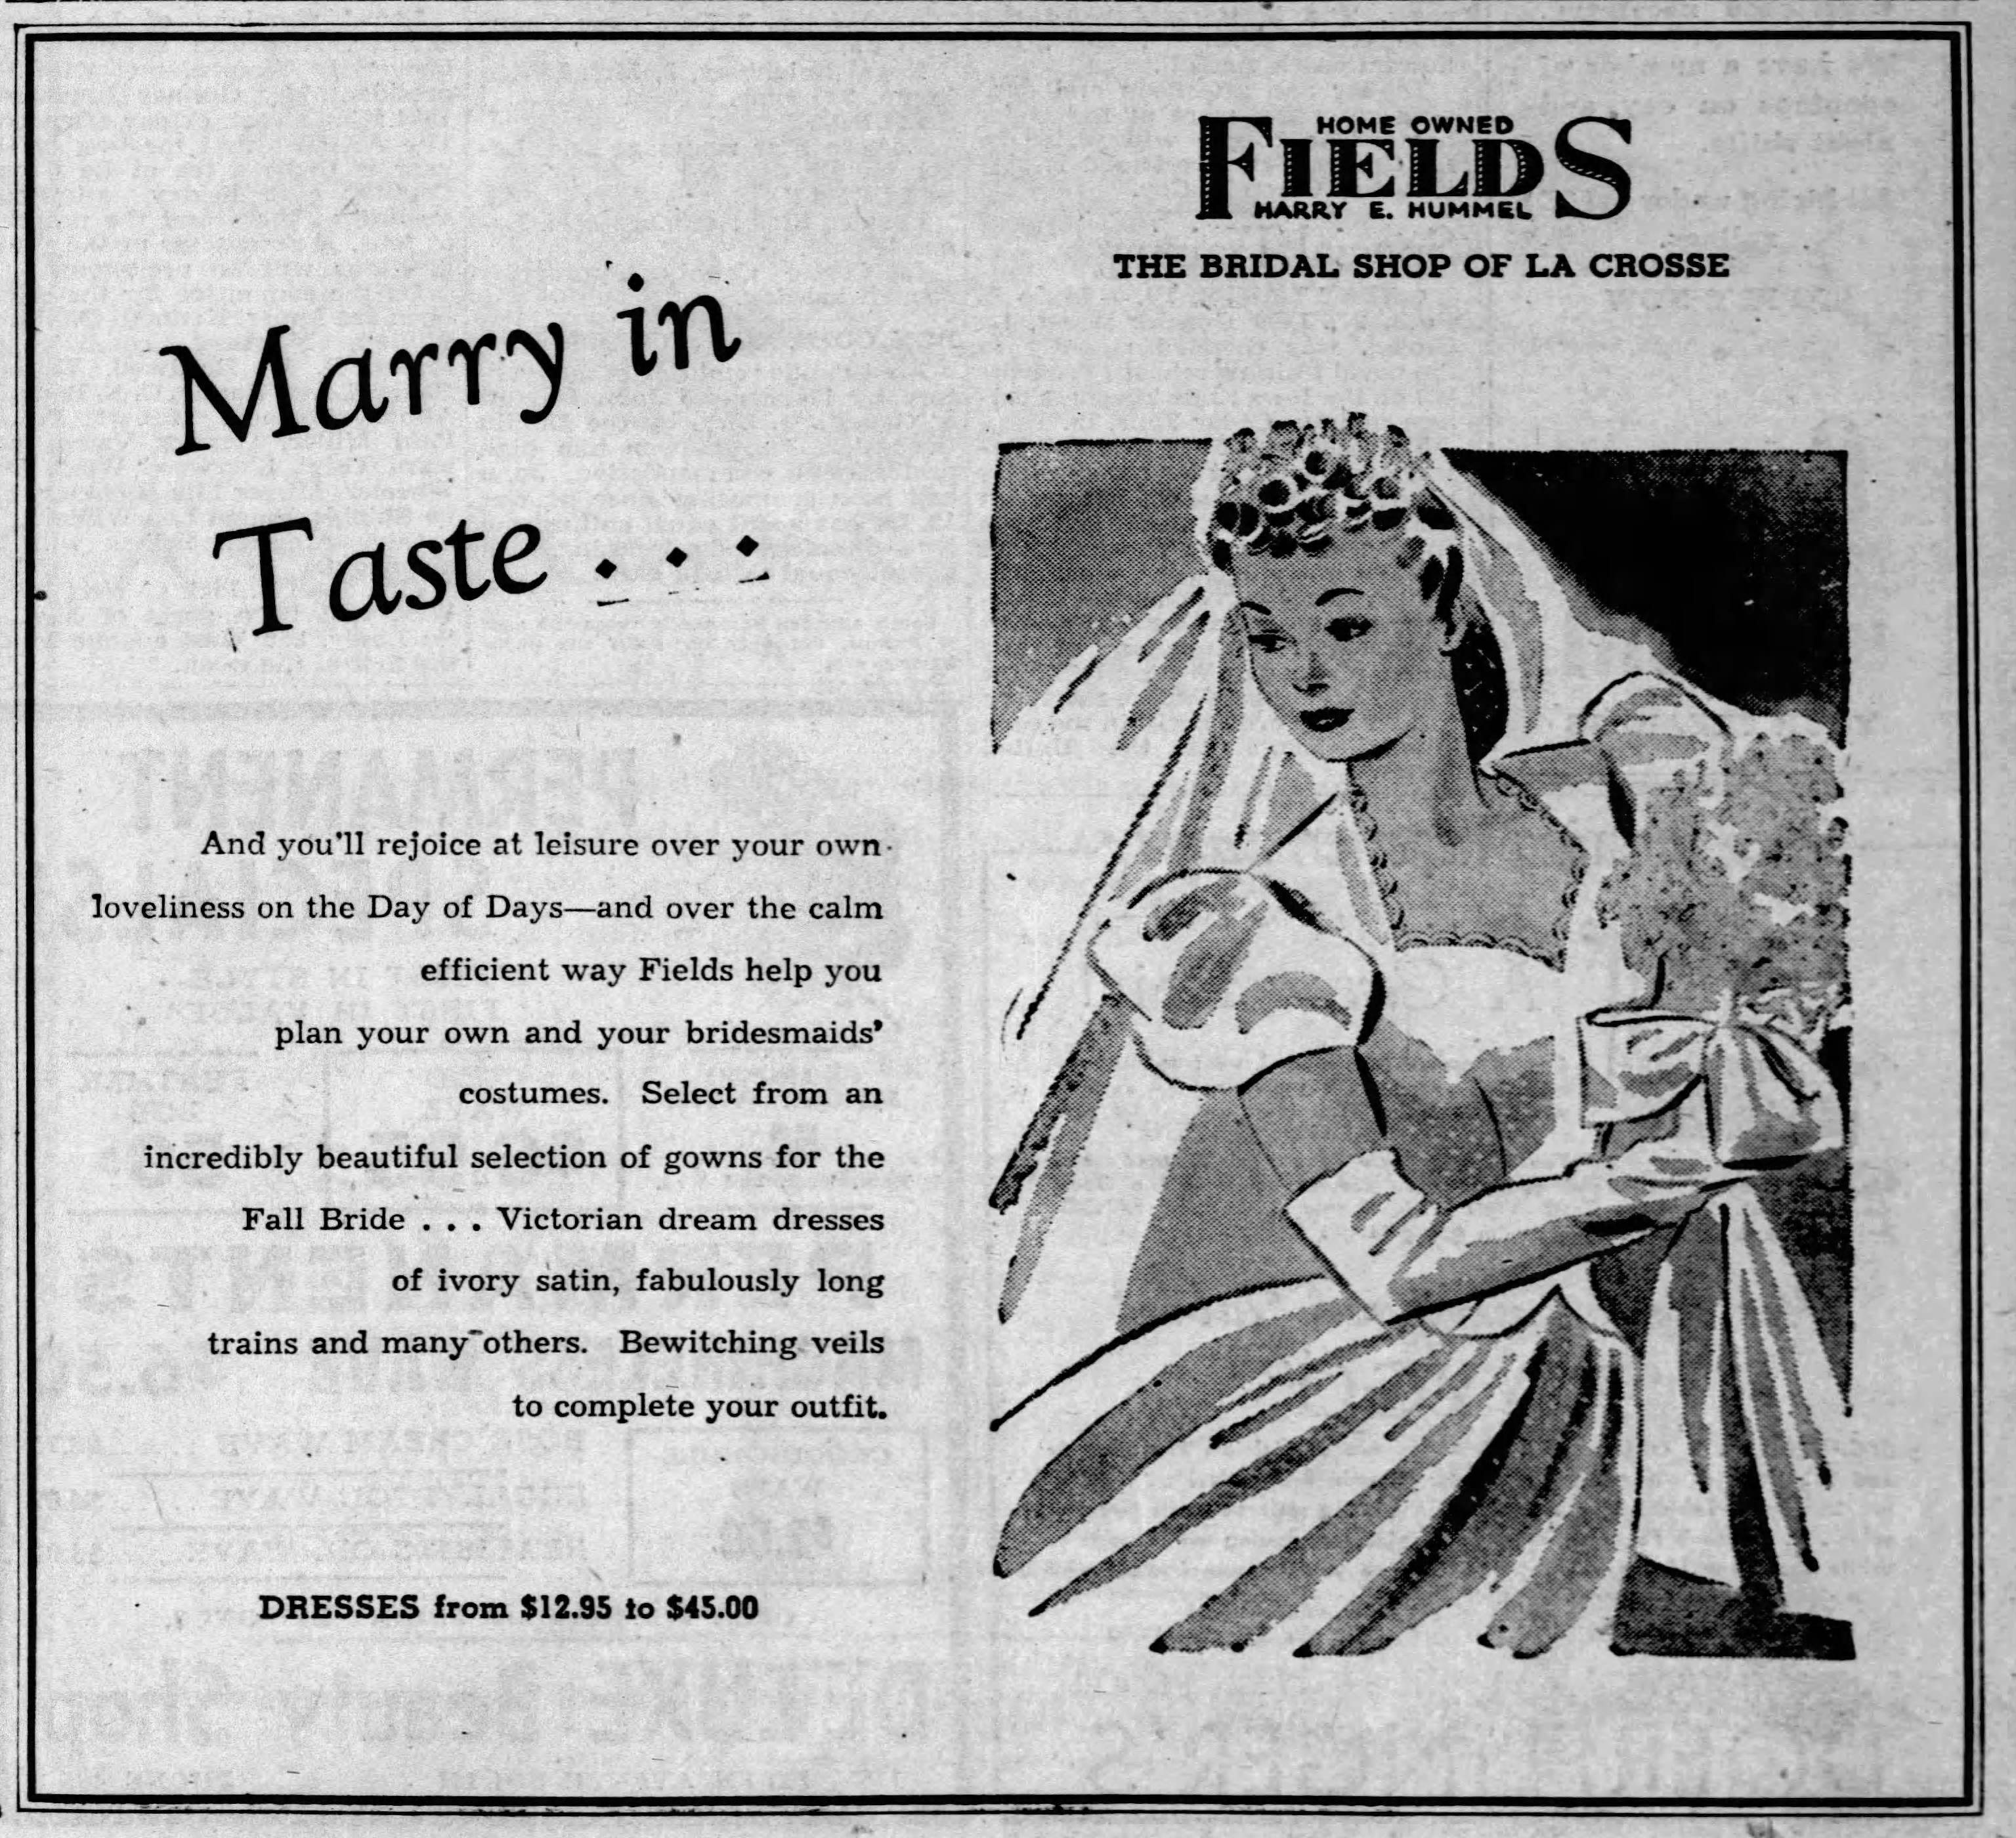
\includegraphics[width=0.85\linewidth,height=\textheight,keepaspectratio]{images/Akou19.jpg}

}

\caption{Advertisement for Fields on Page Three of the \emph{La Crosse
Tribune}, September 10th, 1944}

\end{figure}%

When the saleswoman returned, she had a tray of tea and cookies, and a
measuring tape around her neck. There was a stack of books on a table by
the door, and she handed one of them to Lila. Embossed in gold letters,
the cover said, \emph{Wedding Embassy Yearbook}. ``This is for you to
keep,'' said the saleswoman. ``It's filled with good advice for planning
your wedding and honeymoon. Do you know what kind of budget you're going
to have?'' As she was talking, she directed Lila to raise her arms
slightly so she could string the tape measure around her chest, waist,
and hips.

Lila was starting to panic about undressing. She felt so embarrassed
about the size of her body and the ugly stretchmarks that now covered
her belly. ``Well,'' Lila stammered, ``I'm not really sure.'' The
saleswoman was being polite, but Lila thought she must be judging her.

``That's alright dear,'' she replied in a cheerful tone. ``Many brides
need time to speak with their parents and fiancé about what they can
afford. I'll finish taking your measurements and then I'll show you some
of the styles for dresses. Do you have a date for the wedding?''

When they left the store an hour later, Lila was exhausted. The
saleswoman, whose name was Katherine, was like a human windstorm. She
had never stopped moving; she barely stopped talking long enough to hear
Lila's responses. Mercifully, she had not asked Lila to undress. She
explained that the dresses were just samples; once they received a
deposit, they would make her dress to order. (Unless she was in a hurry?
The saleswoman looked relieved that Lila was not.) It was hot that
afternoon and the baby was getting fussy. Myrtle suggested that they
hire a taxi and go back to the house to wait for Herman. Lila agreed and
handed her a dollar for the fare.

Lila had mixed feelings about being in her old neighborhood. She missed
the bustle and excitement of the city, but she had not seen anyone from
her family in more than three months. Veda had mailed several letters to
Myrtle's house, but Lila couldn't bear to open them. She was still
overwhelmed with anger and shame. Did the Slabacks have any idea that
she was in West Salem? Probably not. She wondered if any of them would
attend her wedding.

\begin{figure}[H]

{\centering 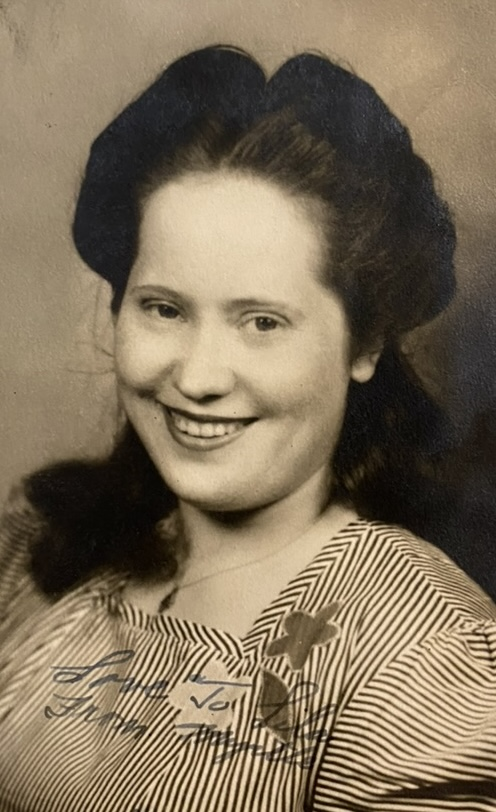
\includegraphics[width=0.5\linewidth,height=\textheight,keepaspectratio]{images/Akou20.jpeg}

}

\caption[Self-portrait that Myrtle gave to Lila around the time of her
marriage in 1944]{Self-portrait that Myrtle gave to Lila around the time
of her marriage in 1944; the handwritten inscription says, ``Love to
Lila, From Myrtle''}

\end{figure}%

\section{Notes}\label{notes-36}

In 1944, when Lila was an unwed mother who kept her baby and did not
give it up for adoption, that was an extremely unusual decision for a
woman in the United States to make. Such babies were described as
``illegitimate'' and their mothers were often denied support by their
families, communities, and the government. So why did Edward and Alice
Schneider accept Lila into their family, knowing that she was pregnant
and Herman was not the biological father? I suspect the main reason is
that Herman was already thirty-six years old and had never been married.
Lila gave him an opportunity to have an instant family and was clearly
fertile; she could have more children with Herman. It's also possible
that the Schneiders' faith motivated them to be charitable; they may
have viewed the marriage as saving Lila and her baby from adoption.

My description of Lila's birth is based on my own experiences with
unmedicated childbirth. Although I had grown up in a small town, I
remember being shocked by the absence of sound when I moved from
St.~Paul, Minnesota to Bloomington, Indiana in 2004. It was so quiet
that I could hear my husband's heart beating in the middle of the night.
Large masses of frogs can be surprisingly noisy!

Fields department store was new to La Crosse. With a major army base
nearby (Fort McCoy), I imagine there were a lot of brides in La Crosse
who needed quick wedding dresses in the 1940s. I bought a 1939 copy of
the \emph{Wedding Embassy Yearbook} online from a used bookseller.

For more information, see Cutright. Phillips\footnote{\citeproc{ref-cutright1972a}{{``Historical
  and Contemporary Trends in Illegitimacy,''} \emph{Archives of Sexual
  Behavior} 2, no. 2 (1972): 97--118}.}, Howard\footnote{\citeproc{ref-howard2008a}{\emph{Brides,
  Inc.}}}, Judith Walzer Leavitt\footnote{\citeproc{ref-leavitt2016a}{\emph{Brought
  to Bed: Childbearing in America, 1750--1950} (Oxford University Press,
  2016)}.}, and York\footnote{\citeproc{ref-york2012a}{\emph{Bridal
  Fashion 1900--1950}}.}.

\bookmarksetup{startatroot}

\chapter{Chapter Thirty-Five}\label{chapter-thirty-five}

Since Myrtle was the one who told Veda about the baby and the date for
the wedding, Lila was surprised to see Veda and Red as she walked down
the aisle at Christ Lutheran. It was a sunny day in October, and the
small church was bathed in a rainbow of light. Veda was holding a tiny
baby, and Red was holding David. He had grown so much in the last few
months. Myrtle was sitting next to them holding her namesake. She smiled
as Lila walked past arm-in-arm with Herman's father, Edward. Herman was
wearing a three-piece suit that he had borrowed from John, the same suit
John had worn for his own wedding.

While Lila was living with his parents, Herman had stopped by many
times. Everyone said that he adored her, but he was so quiet\ldots Lila
still felt like she barely knew him. He was working on a farm near
Hamilton, just outside of West Salem. The farmer knew that Herman was
getting married but didn't want to lose such a reliable and hard worker,
so he offered him a small house on the property. Herman had given it a
fresh coat of white paint and built some furniture; the Schneiders had
added a mattress and some linens. Like the house in West Salem, it did
not have running water or electricity. She would have to do everything
herself---hauling water for the laundry and heating it over the
wood-fired stove, lighting the kerosene lamps (which could explode and
start a fire), canning vegetables without a second pair of hands---it
was more work than she had ever done before, plus now she had a child.
Was this really going to be her new life? Alice had patiently taught her
some skills for living in the country like how to kill and pluck a
chicken, but she wasn't sure it would be enough.

Lila had gone back to Fields twice to order a dress and have it fitted,
riding with Viola as she drove into the city to visit Myrtle. She was
grateful for the money she had earned as a waitress. It was the only
reason she could afford the dress. She was sure that Alice would have
offered to make her one, but she had already been so kind and generous.
Lila didn't want to add to her burden. The dress was soft pink, with
short sleeves and a long hemline. Everyone knew that white was for
virgins. It did not have a train or a veil; the thought of having fabric
over her face made Lila feel claustrophobic. The last fitting had been
just two weeks before the wedding, but the dress was already a little
loose. Her hair was falling out at an alarming rate; it felt thin when
she brushed it on the morning of the wedding. Gladys had picked some
white roses and pinned them to her dress. Herman also had one on his
suit.

\begin{figure}[H]

{\centering 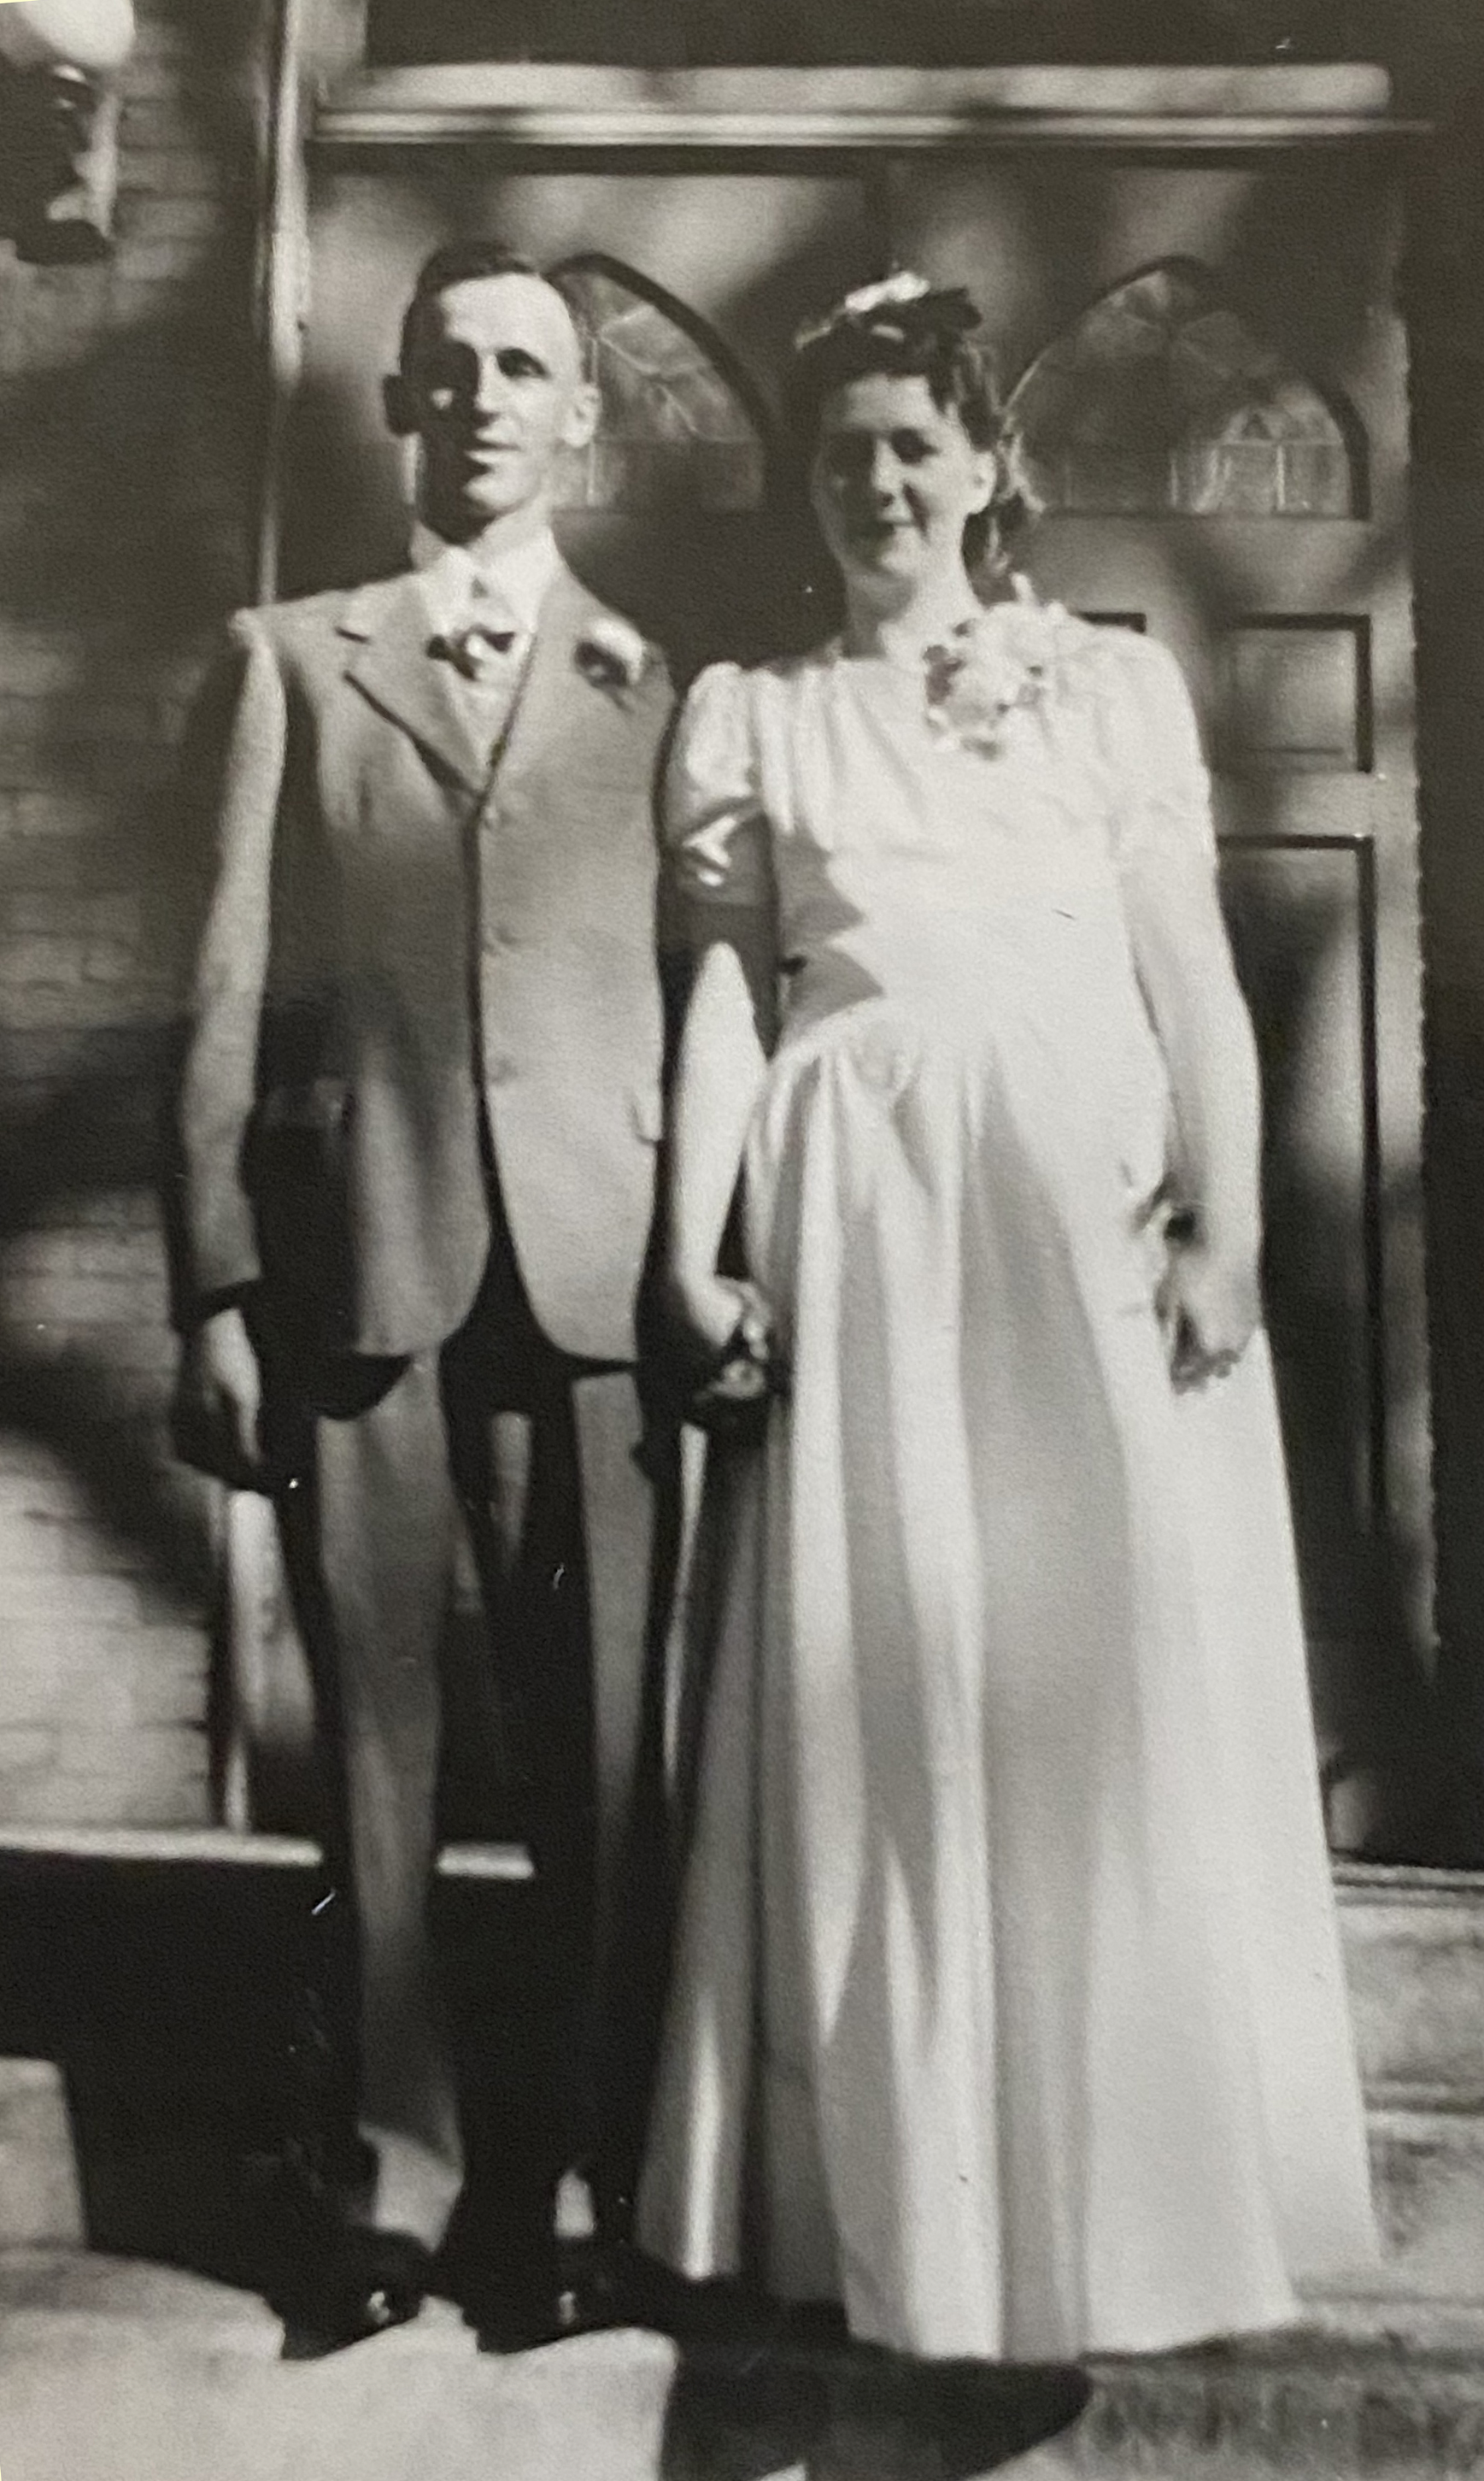
\includegraphics[width=0.5\linewidth,height=\textheight,keepaspectratio]{images/Akou21edit.jpg}

}

\caption{Herman and Lila Schneider on their wedding day, October 14,
1944}

\end{figure}%

During the ceremony, Lila was in a haze. She followed the pastor's
instructions (``With this ring, I thee wed\ldots{}''), but it was like
she was watching someone else get married, not going through it herself.
Herman had purchased the ring. It was a simple gold band, and it was
warm from being in his pocket. As Herman kissed her and took her arm so
they could walk down the aisle as man and wife, Lila was suddenly
grateful for his steady and reassuring presence.

They held hands as they greeted everyone outside; it was not a large
group. After lunch, they would be driving to their new home. Lila heard,
``Let me take your picture!'' The request was from Red. He was holding a
camera. Lila thought that it must be new; she had not seen it before.
Veda walked over and gave Lila a little sideways hug with her right arm.
In her left arm, she was holding the baby. ``Boy or girl?'' said Lila
pleasantly, as if the fight between them had never happened.

``Patricia,'' she said with a flat expression on her face. ``Patty for
short. Myrtle introduced us to your little girl.''

Gladys was standing next to them, and Lila said, ``This is my sister.''

``Oh,'' said Gladys, ``Pleased to meet you,'' but then immediately
walked away. (Months later, Gladys confessed that she had not been
pleased. ``Where was she when you were pregnant and needed help? If I
were her, I wouldn't have shown my face at your wedding.'')

Veda said, ``Red and I have decided to sell the house. He has a new job
as a fireman\ldots we're moving to a neighborhood closer to the
station.'' Lila was stunned. It was the house her father had built. The
house where they had grown up. How could they just walk away like that?
It felt like a rejection. Veda continued, ``We have a crate in the car
with the rest of your things. Where would you like us to put it?''

Herman had been listening to the conversation and said, ``I'll put it in
my truck.'' He let go of Lila's hand and disappeared with Red.

The day was supposed to be happy, but Lila suddenly felt sick to her
stomach, ``I need to feed Myrtle and then I think it's time for lunch.''
Why did Veda have to tell her this news at her wedding? It could have
waited.

``We're not going to stay,'' said Veda as Lila walked away.

Nora was holding Myrtle Joyce and asked Lila what was wrong, but by then
Lila was so upset that she was unable to speak. Nora handed Lila a
handkerchief and said quietly, ``The pastor has an office next to the
sanctuary. I'll let you in and then give you a little privacy. I'll let
Gladys know where to find you when it's time for lunch.''

As promised, Veda and Red did not stay. Lila's out-of-wedlock birth had
caused such a rift in the Slaback family that Veda was the only one who
attended her wedding. Lila had done the right thing and found someone to
marry, but it didn't erase the shame. When Lila realized later what had
happened, she wondered if her parents and siblings would ever forgive
her.

A friend of the Schneider family had made the wedding cake. It had many
thin layers and was soaked with honey. It looked like the rings of a
tree when it was cut open. Gladys leaned over and said, ``This is called
a \emph{Baumkuchen}, and it's a special thing for weddings\ldots it's
for sweetness and good luck.'' There was no music and no dancing, but
the Schneiders gave her a warm welcome to their family. Lila Schneider.
Her new name.

When they arrived at the little white house, Lila was exhausted. It only
had two rooms. In the front was the kitchen, which had a table and
chairs, some shelves, and a wood-fired stove. In the corner was a tub
for washing; the outhouse was in the back. There was a yellow curtain in
the doorway to the bedroom. Lila pushed it aside and put the baby in the
crib; she had fallen asleep during the drive. Herman set the crate on
the table and turned to give her a hug. He was solidly built. Lila
softened into his chest and sighed. For a little while, they just stood
there embracing, not saying or doing anything.

Finally, Herman said, ``I need to milk the cows. Why don't you take a
little nap?''

``That sounds good,'' Lila said.

They walked into the bedroom, and she sat on the bed. He took off the
suit and carefully folded the jacket and pants. He would have to return
them to John. He also took off the shirt and shoes that were his
``Sunday best.'' For a moment he stood there in his undergarments. Lila
wished that he would lie down with her. His warmth was comforting, and
she wanted to know him better; she wanted him to know her too. A husband
and wife should be intimate. Instead, he put on a flannel shirt and a
pair of overalls. ``I won't be long,'' he said as he got dressed. He
smiled at her and left the house without saying another word.

When he was gone, Lila went to the kitchen and looked in the crate. On
top was her doll, Elizabeth. She had been put away for several
years\ldots Lila remembered holding her in her lap as they rode the
train to La Crosse. She smiled and set the doll aside. She would give it
to Myrtle when she was ready for toys. Under the doll was her uniform
for the Girl Reserves. She rolled her eyes and wondered why she had kept
it. Then she realized that she could reuse the cloth\ldots she would
make more diapers for the baby. Aunt Hattie would be horrified. Her
rubber boots would be useful on the farm\ldots so would the
undergarments and dish towels. For a moment she was grateful that Veda
had delivered the crate. Then she noticed the red uniform from
Carroll's. She held the dress up to her body and realized there was no
way it would fit. For a moment she thought of cutting it up, but then
she carefully tucked the shoes, the dress, and the shrug into the bottom
drawer of the dresser. She wasn't ready to give that memory up. Feeling
tired again, she put the empty crate by the stove. She took off her
shoes. They were beautiful satin slippers that she would wear as house
shoes until they fell apart. She took off her wedding dress and draped
it over Herman's suit on the dresser. She would have to wash it before
putting it away. Dressed in only her slip and camisole, she laid down on
the bed and fell asleep.

Herman returned not long after she woke up. He was carrying a large pan
with a lid. The farmer's wife, Evelyn, had roasted a whole chicken with
potatoes and carrots as a gift. It smelled delicious. Herman lit the
kerosene lamp that was sitting on the table. He went outside again, and
Lila wondered what on earth he was doing. He returned with some wood,
which he used to start a fire in the stove. The day had been warm, but
the night would be cold. He pulled two plates, two forks, and a large
knife from the shelves and set them on the table next to the roasting
pan.

Lila was feeding the baby. ``Would you bring me a glass of water?''

``Sure,'' said Herman. ``Just a moment.'' He grabbed a pail and went
outside.

The water was ice cold. ``Why is it so cold?'' she asked.

``There's a pump in the yard, but the water is from an underground
spring.''

It was like drinking water straight from an icebox.

The next day, Herman did not work. Although it was harvest season, Vilas
had hired a local boy to help so Herman and Lila could have a little
time together as a new couple. If Lila had realized what a hard worker
Herman was, she would have savored that day so much more. Before going
to bed, he had stoked the fire and put a pot of water on the stove.
After spending the morning in bed, they ate the rest of the chicken, and
Lila washed the pan with a little of the hot water. Herman had purchased
some basics for the house---flour, sugar, salt, coffee---but he said
that Evelyn would send some smoked ham and jars of fruit and vegetables
for the winter. He proposed that they go fishing and pick a squash from
the garden on the way back.

Lila had never been fishing before. She knew people fished along the
river in La Crosse, but it was not something her family did. It was
another beautiful day. The trees were brilliant shades of red, yellow,
and orange; soon they would be bare again. Lila bounced Myrtle on her
knee as she sat on a boulder by the creek and watched Herman fish. He
quickly caught four trout and they walked back to the house. Lila
watched as he gutted and scaled the fish; he made it look so easy. He
told her to wait until the pan was blazing hot before adding the butter
and the fish. It made the fish so crispy and good that she ate every
morsel and sucked the bones and tail.

Herman was always quiet, but when they made love again (after the baby
went to sleep), he was completely silent. He fell soundly asleep without
saying another word. By the time Lila woke up the next morning, he had
already left to milk the cows.

\section{Notes}\label{notes-37}

Living without running water and electricity is a lot of work. Growing
up in the city meant that Lila had a lot to learn about living in the
county. I was shocked the first time I stayed in a house that didn't
have plumbing (for a family vacation in northern Wisconsin in the
1980s). It makes even the most ordinary chores---like washing the
dishes---complicated and time-consuming.

The idea of wearing white for a wedding was introduced in the
mid-nineteenth century by Queen Victoria. Although it took several
decades for white to become the standard in the United States, by the
1940s many Americans saw the ``white wedding'' as a sign of the bride's
virginity or even as a religious requirement. Since Lila had recently
given birth, I imagine she felt pressure not to wear white. The
photographs of her wedding day are black-and-white, so I know the
silhouette but not the color. My description of Lila's post-pregnancy
weight loss and hair loss is based on my own experience with an
undiagnosed thyroid disorder. Lila had the same condition.

I was two years younger than Lila when I got married, but I was thrilled
to shed my childhood name (Heather Wall) and take the name of my
husband's family (Akou). Unlike middle-class families with cars and
vacation time, Herman and Lila could not afford a honeymoon. In this
chapter, Lila is immediately confronted with the pleasures and
difficulties of farm life.

For more information, see Sylvia M. Henderson\footnote{\citeproc{ref-henderson2001a}{{``Baumkuchen,''}
  \emph{Gastronomica} 1, no. 2 (2001): 90--92}.}, Katherine
Jellison\footnote{\citeproc{ref-jellison2008a}{\emph{It's Our Day:
  America's Love Affair with the White Wedding, 1945--2005} (Lawrence:
  University Press of Kansas, 2008)}.}, Lowry Nelson\footnote{\citeproc{ref-nelson1954a}{\emph{American
  Farm Life} (Cambridge: Harvard University Press, 1954)}.}, and Rachel
Ann Rosenfeld\footnote{\citeproc{ref-rosenfeld2017a}{\emph{Farm Women:
  Work, Farm, and Family in the United States} (Chapel Hill: University
  of North Carolina Press, 2017)}.}.

\bookmarksetup{startatroot}

\chapter{Chapter Thirty-Six}\label{chapter-thirty-six}

Although Lila was never much of a reader, a few months later she was
cleaning the house and noticed the \emph{Wedding Embassy Yearbook} from
Fields. As she leafed through it, she read the author's advice about
``honeymoons'':

\begin{quote}
If your honeymoon is to be spent inside U.S. borders, you will probably
be driving or taking a train. Remember food and lodging if you drive.
Railroad diners are not cheap. Figure such costs ahead of time. If
you're lucky enough to be honeymooning on a cruise ship or a trip to
foreign shores, you must figure in transportation for two from your
hometown to New York or San Francisco and back. Things like that are
easy to overlook.
\end{quote}

It was ridiculous advice. Nobody she knew had ever been to New York or
San Francisco. She wasn't even sure what state San Francisco was in.

For most of her life, Lila had been a listener. At school she listened
to her teachers; at dinner she listened to her parents and older
brothers. At work, her listening skills made her an excellent waitress.
She never forgot an order. Living with Herman was different because he
said so little. Lila found it unnerving. Desperate for someone to
communicate with, she tried making friends with Evelyn. To her
disappointment, she found that Evelyn was always on the go. As the
president of the La Crosse County Homemakers Association (and mother of
only one child), she was constantly gardening, sewing quilts, and making
pies. A wall in their house was filled with ribbons that she had won at
the county fair. Lila found Evelyn intimidating.

She begged Herman to show her how to drive the truck. If she could
drive, she could visit Alice and Gladys or go shopping with Myrtle in La
Crosse. He promised that he would as soon as the snow was gone. That
winter was one of the longest she had ever known. It should have been a
happy time with a new baby and a new husband. Instead, she felt
isolated, bored, and sad. Every day was basically the same. Herman would
be gone by the time she woke up. He would come back with a fresh
canister of milk, which they would drink with slices of bread from the
day before. Sometimes there would be eggs, but the chickens did not lay
as much in the winter. At first, she marveled over the different colors
of the shells---white, light brown, darker brown with speckles, and pale
green (the flock belonged to Evelyn, and she had many different breeds
of chickens)---but after a few weeks, the novelty wore off. For lunch,
she made grilled cheese. For dinner, she might open one of the jars.
They had many dinners of oatmeal with fruit, milk, and blackstrap
molasses. Myrtle Joyce was crawling all over the house. Lila missed
listening to the radio and taking walks around La Crosse. She could walk
down the road as much as she liked (and often did), but there was so
little to see\ldots just endless farmhouses and empty fields.

On Sundays, they went to church with Vilas and Evelyn. It was a one-room
Lutheran church on Gills Coulee Road. Most of the congregants had grown
up together. As Lila later confessed to Myrtle, she stood out like a
sore thumb. She didn't know the words to the service. She didn't know
any of the songs. Some churches had books to help people follow along
with the service, but this one did not. There was no need since they
knew what to do.

After the first week, the pastor told her that if she wanted to join
everyone for Holy Communion, she would need to take confirmation
classes. The thought filled Lila with dread. She had never been a good
student. So, every two weeks when it was time for communion, she stayed
in her pew, held the baby, and tried to make herself inconspicuous. She
noticed that the other mothers with small children would pass them
around so everyone could take turns going up to the altar, but nobody
offered to hold Myrtle Joyce. Was it because she was not Lutheran or
because they questioned whether Herman was the father? Lila had no idea.

Since it was easily her best outfit, she wore her wedding dress every
Sunday to church. Other young women did the same thing, but it was
making Lila feel extra self-conscious. She was losing weight from the
pregnancy and the dress was growing more and more loose every week. Lila
did her best to take it in without a sewing machine, but she was hardly
a professional seamstress. She was sure that everyone could tell and was
silently evaluating her. In February, Lila stopped losing weight; she
was pregnant again. Her first thought was how glad she was that she
could stop fussing with the dress.

Herman was thrilled by the news that she was expecting. One muddy day in
April she took a walk with Myrtle Joyce. Evelyn was outside feeding the
chickens and asked where Lila was planning to deliver the baby. ``I
suppose with Herman's mother in West Salem. That's where Myrtle Joyce
was born.'' Evelyn paused with her hand in the pail of grain. ``It's not
safe to give birth at home\ldots do you know how many women die of
infections? You really should go to the hospital.'' Lila quickly put the
conversation out of her mind, but Evelyn did not.

A few weeks later, Herman asked Lila if she wanted to stay in La Crosse
until the baby was born. Evelyn had pressured her husband into talking
with Herman.

``I could stay with Myrtle if she's willing.''

Herman paused to think. ``Carl is coming home from Europe soon. What
about your family?''

Lila relished the thought of spending a little time in La Crosse, but
her heart sank when he mentioned her family. Who was she supposed to
stay with? Veda and Red? Lyle and Allene? For days, the possibilities
tumbled through her mind. She was so distracted that one evening she
accidentally burned the potatoes. She burst into tears, but Herman said
nothing. His silence confused her. Did he not care about dinner? Did he
not care about her? She wished that he would yell or slam the door.
Anything would be better than silence.

It was calving season and Herman was even busier than usual. Myrtle was
pulling herself up on the furniture and shuffling around the room. The
trees had come back to life, but Lila was feeling increasingly lifeless.
One day blended into another. There was no friendship, no laughter, no
radio, no movies. It was just endless work. Endless boredom. What was
the point of washing the dishes or making another loaf of bread when she
would just do the same thing the next day and the day after that? There
was no end in sight. She was so tired of drawing water and waiting for
it to boil. She was tired of cooking food that she barely felt like
eating.

\section{Notes}\label{notes-38}

At the time of the 1940 census, Herman was working as a ``hired hand''
for Vilas and Evelyn Young on a farm near Hamilton, Wisconsin
(population 1,342). From archival newspapers, I learned that they were
quite a busy and impressive couple. Vilas had finished high school and
enjoyed breeding cattle for show; he was a long-time judge of livestock
at the La Crosse County Fair. Evelyn had attended college for two years
and served as president of the La Crosse County Homemakers Association.
As a highly educated woman, she likely would have been exposed to
consumer trends like medicalized childbirth. I don't know if she
influenced Lila, but I do know that Lila's second child was born in a
hospital and not at home. The time she spent in the city preparing for
and recovering from the birth would have changed her relationship with
her first child and husband---unintended collateral damage, even if the
birth was physically safer.

In rural areas (even today), churches can be wonderful places to connect
and gain support. There was just one problem for Lila: she didn't know
how to fit in. Having grown up in a non-religious family, she didn't
know any of the songs, rituals, or rules. She probably felt
self-conscious about being an outsider with a newborn of questionable
status. It would have been easy for her to feel judged and ``take things
the wrong way,'' even if that was not the intent of the other
churchgoers. Herman knew what to do in church, but (even if he was
willing to teach Lila) many churches are segregated by gender in their
activities. This chapter draws on my own experience of fitting into a
religious community that is completely different from the one where I
grew up.

For more information, see Carolyn M. Goldstein\footnote{\citeproc{ref-goldstein2012a}{\emph{Creating
  Consumers: Home Economists in Twentieth-Century America} (Chapel Hill:
  University of North Carolina Press, 2012)}.}, Lincoln A.
Mullen\footnote{\citeproc{ref-mullen2017a}{\emph{The Chance of
  Salvation: A History of Conversion in America} (Cambridge: Harvard
  University Press, 2017)}.}, and Raymond DeVries et al.,
eds.\footnote{\citeproc{ref-devries2001a}{\emph{Birth by Design:
  Pregnancy, Maternity Care, and Midwifery in North America and Europe}
  (New York: Routledge, 2001)}.}

\bookmarksetup{startatroot}

\chapter{Chapter Thirty-Seven}\label{chapter-thirty-seven}

One day, Lila was outside drawing water to wash diapers when she noticed
a green truck turning by the barn and heading in her direction. As it
came closer, she could see Gladys waving to her. She hadn't realized how
much she had been drowning in a sea of loneliness until she saw her
face. Her heart leapt as she watched Gladys park the truck and step out.

``I could hardly wait for the roads to dry up so I could come visit
you!''

Lila had already set down the bucket of water and walked over to the
truck. She hugged Gladys and said, ``I'm so relieved to see you!''

Gladys laughed and said, ``That's quite a hug! I guess you really did
miss me.''

They were sitting at the kitchen table when Herman came home for lunch.
He poured a cup of coffee and took one of the sandwiches. ``Hi Gladys.
When did you get here?''

``A little while ago,'' she replied. ``Lila and I are just catching
up.''

When he finished chewing his first bite of the sandwich, he said, ``You
should give Lila a driving lesson. I told her that I would do it, but
I've been busy with the calves.''

When Herman left and they had finished eating, Gladys said,
``Well\ldots are you ready for the lesson?'' Lila could hardly believe
it. It was such a treat just having Gladys for a visit; now she was
teaching her to drive. Gladys picked up Myrtle Joyce, and Lila
cautiously opened the driver's side door and stepped into the cab. She
sat down and Gladys handed her the key. ``Put this in the ignition right
here and then press the button on the dash.'' Lila followed her
directions and the truck roared to life. Speaking louder, Gladys pointed
out the clutch, the brake, and the gas pedal. ``We probably won't go far
today\ldots the first thing is to learn how to shift and use the
clutch.'' The truck rolled forward a bit and then lurched to a stop.
Lila was horrified, but Gladys was laughing. ``Everyone does that the
first few times. It takes a little practice to get it right.'' It wasn't
long until they were out on the road. When they finished the lesson,
Gladys opened the door of the glove box and pulled out an envelope.
``This is for you,'' she said. ``It's an application for a driver's
license. You just have to fill it out and give them fifty cents.''

That Sunday, Herman said he wanted to go to West Salem for church. As
they walked to the truck, he handed the key to Lila. ``You can be the
driver this time.'' Lila blushed as he took Myrtle Joyce and opened the
passenger door. Herman gave her directions to Christ Lutheran; she was
proud of herself for only stalling the truck once. Alice, Nora, and
Gladys were happy to see her again. Since her wedding dress no longer
fit, she had worn her favorite blue maternity dress. It was obvious that
she was expecting again. During lunch she told Nora and Gladys that
Herman was encouraging her to go to La Crosse for the birth. Nora said,
``You could come here, but I'll ask Viola for ideas.'' A few weeks
later, Nora said, ``I have good news for you! Viola's parents offered to
let you stay at their house\ldots you can go to St.~Ann's for the
birth.'' St.~Ann's was the maternity hospital for St.~Francis, where
Lila had learned of her first pregnancy.

It was a hot day in August when Herman drove her to the Johnson house.
It was strange (but also a relief) to be away from Myrtle Joyce. They
had taken her to West Salem to stay with Alice until Lila was home with
the baby. Since the day she was born, Lila and Myrtle Joyce had never
been apart for more than a few hours; now they would be apart for a few
weeks.

When Herman and Lila arrived in La Crosse, Viola's mother, Bertha, was
at home with her three youngest daughters. Evelyn and Rosemary were
teenagers; Ruth was only four years old. Bertha showed Lila where she
would sleep, then said she needed to go. She and her husband had opened
a bar and she needed to help with the evening rush. Rosemary turned on
the radio and suggested that they play a game of cards. ``It takes four
people for euchre, so let's play gin rummy.'' Evelyn agreed and pulled a
deck of cards and a notepad from a drawer in the kitchen.

The next day, Myrtle dropped by. Carl had been home for almost two
months, and she was still giddy about it. They decided to take a
streetcar downtown to see the new Abbott and Costello movie. On the way
she talked non-stop; it made Lila giggle. She missed being close to
Herman, but she had also missed La Crosse---hearing the traffic,
smelling the river, feeling dwarfed by the tall buildings, and imagining
the stories behind the snippets of conversation she overheard (``If you
don't tell your mother, Margaret, I will.'') Growing up she had taken
the city for granted, but now it was calling to her like the sirens of
Greek mythology. Her time with the Johnson family passed by too quickly.

\section{Notes}\label{notes-39}

When I did some research for this chapter, I was surprised to learn that
Wisconsin and Alaska were the last two US states to require examinations
for new drivers (1956). In the 1940s when Lila was a young adult,
drivers could get a license just by applying and paying a small fee. The
scene where Gladys teaches Lila to drive is based on my own experiences
learning to drive a car with manual transmission. Safety features like
seatbelts and car seats for children were unheard of in the 1940s.

In this chapter, Lila stays with the Johnson family (Myrtle and Viola's
parents) before the birth of her second child. Being in La Crosse makes
her nostalgic for city life. This is foreshadowing for upcoming
chapters.

For more information, see Federal Highway Administration Office of
Highway Information Management\footnote{\citeproc{ref-fwha1997a}{{``Highway
  Statistics Summary to 1995''} (Washington, DC: Federal Highway
  Administration, 1997),
  \url{https://www.fhwa.dot.gov/ohim/summary95/dl230.pdf}}.}, Charles J.
Kahane\footnote{\citeproc{ref-kahane1986a}{{``An Evaluation of Child
  Passenger Safety: The Effectiveness and Benefits of Safety Seats''}
  (Washington, DC: National Highway Traffic Safety Administration,
  1986)}.}, and Ralph Nader\footnote{\citeproc{ref-nader1965a}{\emph{Unsafe
  at Any Speed: The Designed-in Dangers of the American Automobile} (New
  York: Grossman Publishers, 1965)}.}.

\bookmarksetup{startatroot}

\chapter{Chapter Thirty-Eight}\label{chapter-thirty-eight}

When the baby was born, Lila decided to name him after both of his
grandfathers---John Edward Schneider. Herman was so proud when he held
his son for the first time. He embraced Lila and told her that he
couldn't wait to have everyone back home. After a week in the hospital,
Carl and Myrtle drove her back to the farm.

John was such an easy and sweet baby. Edward and Alice were overjoyed
about their oldest son's growing family. Herman and Lila began spending
almost every Sunday in West Salem. Gladys said it was too bad they
didn't live a bit closer. Although Herman had to get back to the farm to
help with milking, Lila often stayed behind for the rest of the day.
Alice enjoyed spending time with her grandchildren, and Lila enjoyed
spending time with Gladys. She was going to parties at Camp McCoy and
dating a veteran named Carl Schliebe. He had been married before the war
but returned to find that his wife had run off to Minnesota with another
man. Lila and Gladys laughed and talked like they had been close friends
for their entire lives.

One weekend that summer, Gladys said that they should plan a trip to La
Crosse. Lila almost objected that she had nothing to wear, but then she
thought about the red uniform at the bottom of her dresser. When she
tried on the dress the next day, she could hardly believe that it fit.
John was in the crib and Myrtle Joyce was standing on the bed. Lila
twirled around and said (not expecting an answer), ``What do you
think?'' Myrtle Joyce clapped, and Lila laughed. Two weeks later she was
with Gladys driving to La Crosse in the green truck. ``This is so
exciting!'' said Gladys. Lila was excited too. The children were
spending the night with Aunt Nora.

Gladys and Lila had decided to go dancing at the Trocadero, one of the
new nightclubs downtown. It was thirty-five cents to hear the band and
dance from eight p.m. to midnight. The dance floor was already packed by
the time they arrived. It was an ocean of khaki, button-down shirts, and
swirling dresses. As they paid for admission, the band started playing a
new song and the crowd formed a circle to watch two dancers in the
middle. Shockingly, the male dancer was black. His movements were so
fluid and powerful\ldots it was like nothing Lila had ever seen before.
He lifted and spun his partner around like she was weightless. ``Wow,
they can really dance!'' said Gladys. Lila had forgotten where she was
for a second; she was so captivated by the dancers. A young man asked
Gladys to join him and pulled her into the crowd.

Lila was just starting to think about getting a drink when a man came up
behind her and said, ``Lila Slaback.'' She turned, and it was Lloyd. A
shock ran through her body---joy, horror, longing, excitement---she had
never expected to see him again. He obviously didn't know that she was
married now. ``Dance with me, beautiful.'' He held out his right hand,
and Lila took it. Without another word they started dancing. To Lila, it
felt like time had stopped and she was eighteen again---no husband, no
children---just her and Lloyd. His collar was unbuttoned, and he smelled
like cigarettes. His hair was turning gray. His left hand was on her
hip, and Lila wanted him to pull her closer. They danced for two songs
and Lloyd whispered in her ear, ``I've missed you so much.'' Then he
smiled and melted into the crowd, like he had been a mirage. She didn't
see him again for the rest of the night.

Two days later, while Herman was working and the children were napping,
Lila pulled out the letters from Lloyd that she had kept hidden for
years. She should have destroyed them or thrown them away\ldots why
couldn't she just be happy with her life? It was embarrassing that she
could not forget her first love and move on. She unfolded one of the
last letters she had received from Lloyd before her engagement to
Herman.

\begin{quote}
February 5, 1944

Dear Lila, The days have been so cold, but I keep myself warm by
thinking about you. I want to share a bed with you. I want to tell you
dirty jokes and watch your face blush. I want to lick your tits and feel
the shiver of pleasure in your body.

Love, Lloyd
\end{quote}

At the bottom of the letter was a picture of two snails. One was holding
a gun and telling the other snail, ``I'll give you just two days to say
your prayers, buddy!'' She didn't want to miss Lloyd, but she did.

\section{Notes}\label{notes-40}

This chapter represents the best time in Lila and Herman's marriage.
Herman is thrilled to have a son, and an ``easy baby'' gives Lila some
relief. (My children were not easy as babies, so I know how infancy can
be physically and emotionally draining.) Things are going relatively
well for the extended Schneider family.

Dance halls and live bands were popular entertainments in La Crosse in
the 1940s; it was easy for me to find examples and cover charges in the
newspapers (which people living outside of the city would have used to
find such opportunities). La Crosse was hostile to black residents and
visitors; bars and dance halls were unusual spaces where whites (like
Lila) could interact with blacks. They were also spaces where young
people could explore their sexuality.

Lloyd was out of prison in 1946. I have no idea if Lloyd and Lila
reconnected in real life, but this scene gives us more insight into how
Lila feels about the city and her life before marriage. She misses
feeling carefree and sexually desirable.

For more information, see Chad Heap\footnote{\citeproc{ref-heap2009a}{\emph{Slumming:
  Sexual and Racial Encounters in American Nightlife, 1885--1940}
  (University of Chicago Press, 2009)}.}, McBee\footnote{\citeproc{ref-mcbee2000a}{\emph{Dance
  Hall Days}}.}, and Christina Simmons\footnote{\citeproc{ref-simmons2009a}{\emph{Making
  Marriage Modern: Women's Sexuality from the Progressive Era to World
  War II} (Oxford University Press, 2009)}.}.

\bookmarksetup{startatroot}

\chapter{Chapter Thirty-Nine}\label{chapter-thirty-nine}

By January, the snow was so deep that they could no longer drive
Herman's truck. By February, Lila could tell that she was pregnant
again. Veda was sending letters.

\begin{quote}
February 4, 1947

Dear Lila,

This is quite a snowy year, isn't it? When you can drive again you
should visit our new house. Red built a porch. It's such a nice place
for the children to play when the weather is nice. Most of the yard was
a garden when we first moved in, but I've had my fill of weeding and
watering! We planted an oak tree in the middle.

Looy married Jean Shuda last year. Do you remember her? They now have a
baby girl named Rose. Such a pretty name. David will start school in the
fall. It's hard to believe how big the children are getting. Myrtle
Joyce must be getting big too. We should plan a visit to mom and dad's
house so they can see their grandchildren.

Hugs and kisses, Veda
\end{quote}

Lila sometimes wondered why she kept writing. To brag about her house
and family? To make her feel guilty for not visiting more often? Was it
possible that she missed her? Lila hardly ever responded, but Veda kept
writing.

Herman and Lila didn't receive much mail. Since they didn't have a
mailbox, the driver had to knock on their door to make deliveries. He
was an older man who always had a red nose, so Lila thought of him as
Rudolph. She had no idea what his real name was. It made her laugh
inside every time ``Rudolph'' came to the house. Lila decided to write
to Gladys and tell her that she was expecting another baby. It took her
a few weeks to respond with bad news: Alice had suffered a stroke, and
Gladys was taking care of her. It was a shock to everyone. Alice had
been fine---doing her usual activities---and then one morning she fell
trying to get out of bed. When she talked, nobody could understand what
she was saying. It made Lila feel sick to her stomach. Alice had become
dearer to her than her own mother. Herman borrowed a horse from Vilas to
visit his parents; it was the only way to travel in the deep snow.

Lila did not really miss the Slabacks, but Alice's condition made her
think she should give them another chance before it was too late. She
wrote to Veda and said she would visit as soon as the roads were clear.
As she thought about going to La Crosse, she decided that she also
wanted to visit Myrtle and buy some new clothes. If she replaced her
dresses, she could cut up the material and make clothing for the
children. When she told Herman about her plans, he said that he could
use a new pair of rubber boots and gave her forty dollars. It was a lot
of money---enough to buy the clothes, the boots, some additional fabric,
and even to restock the coffee, flour, and sugar. She put the money in
their dresser for safe keeping.

Myrtle and Carl had wasted no time in starting their family. Their first
daughter, Laurie, was born in 1946. By the time Lila was finally able to
drive into the city that spring, they were both visibly pregnant. They
laughed as they hugged over their bellies. Carl was working at the Trane
factory. They were hoping to buy a house in West Salem and raise the
children closer to their cousins. Her younger sister, Rosemary, would be
done with high school soon. Evelyn had married a man from Iowa and moved
to be with him. The Johnson family was shrinking.

As they tried on dresses, Myrtle told her that Viola and John were
getting divorced. Lila was shocked. Divorces happened in the movies, not
in La Crosse. Herman had not said a word about it.

``What happened?'' she said with astonishment.

Myrtle replied, ``Well\ldots I'm not really sure. I think Viola was not
very supportive when John lost his job. She's not the easiest person to
live with.''

Lila nodded and changed the topic, but for weeks she thought about all
of the married couples she knew. She wasn't naïve enough to think that
all adults were nice or that all marriages were fairy tales. One of the
other waitresses at Carroll's had been living alone (even though she was
still married) because her husband had run off with another woman. But
getting divorced in real life? That was nearly unthinkable. Once you got
married, it was supposed to be forever. ``In sickness and health, 'til
death do us part.''

\begin{figure}[H]

{\centering 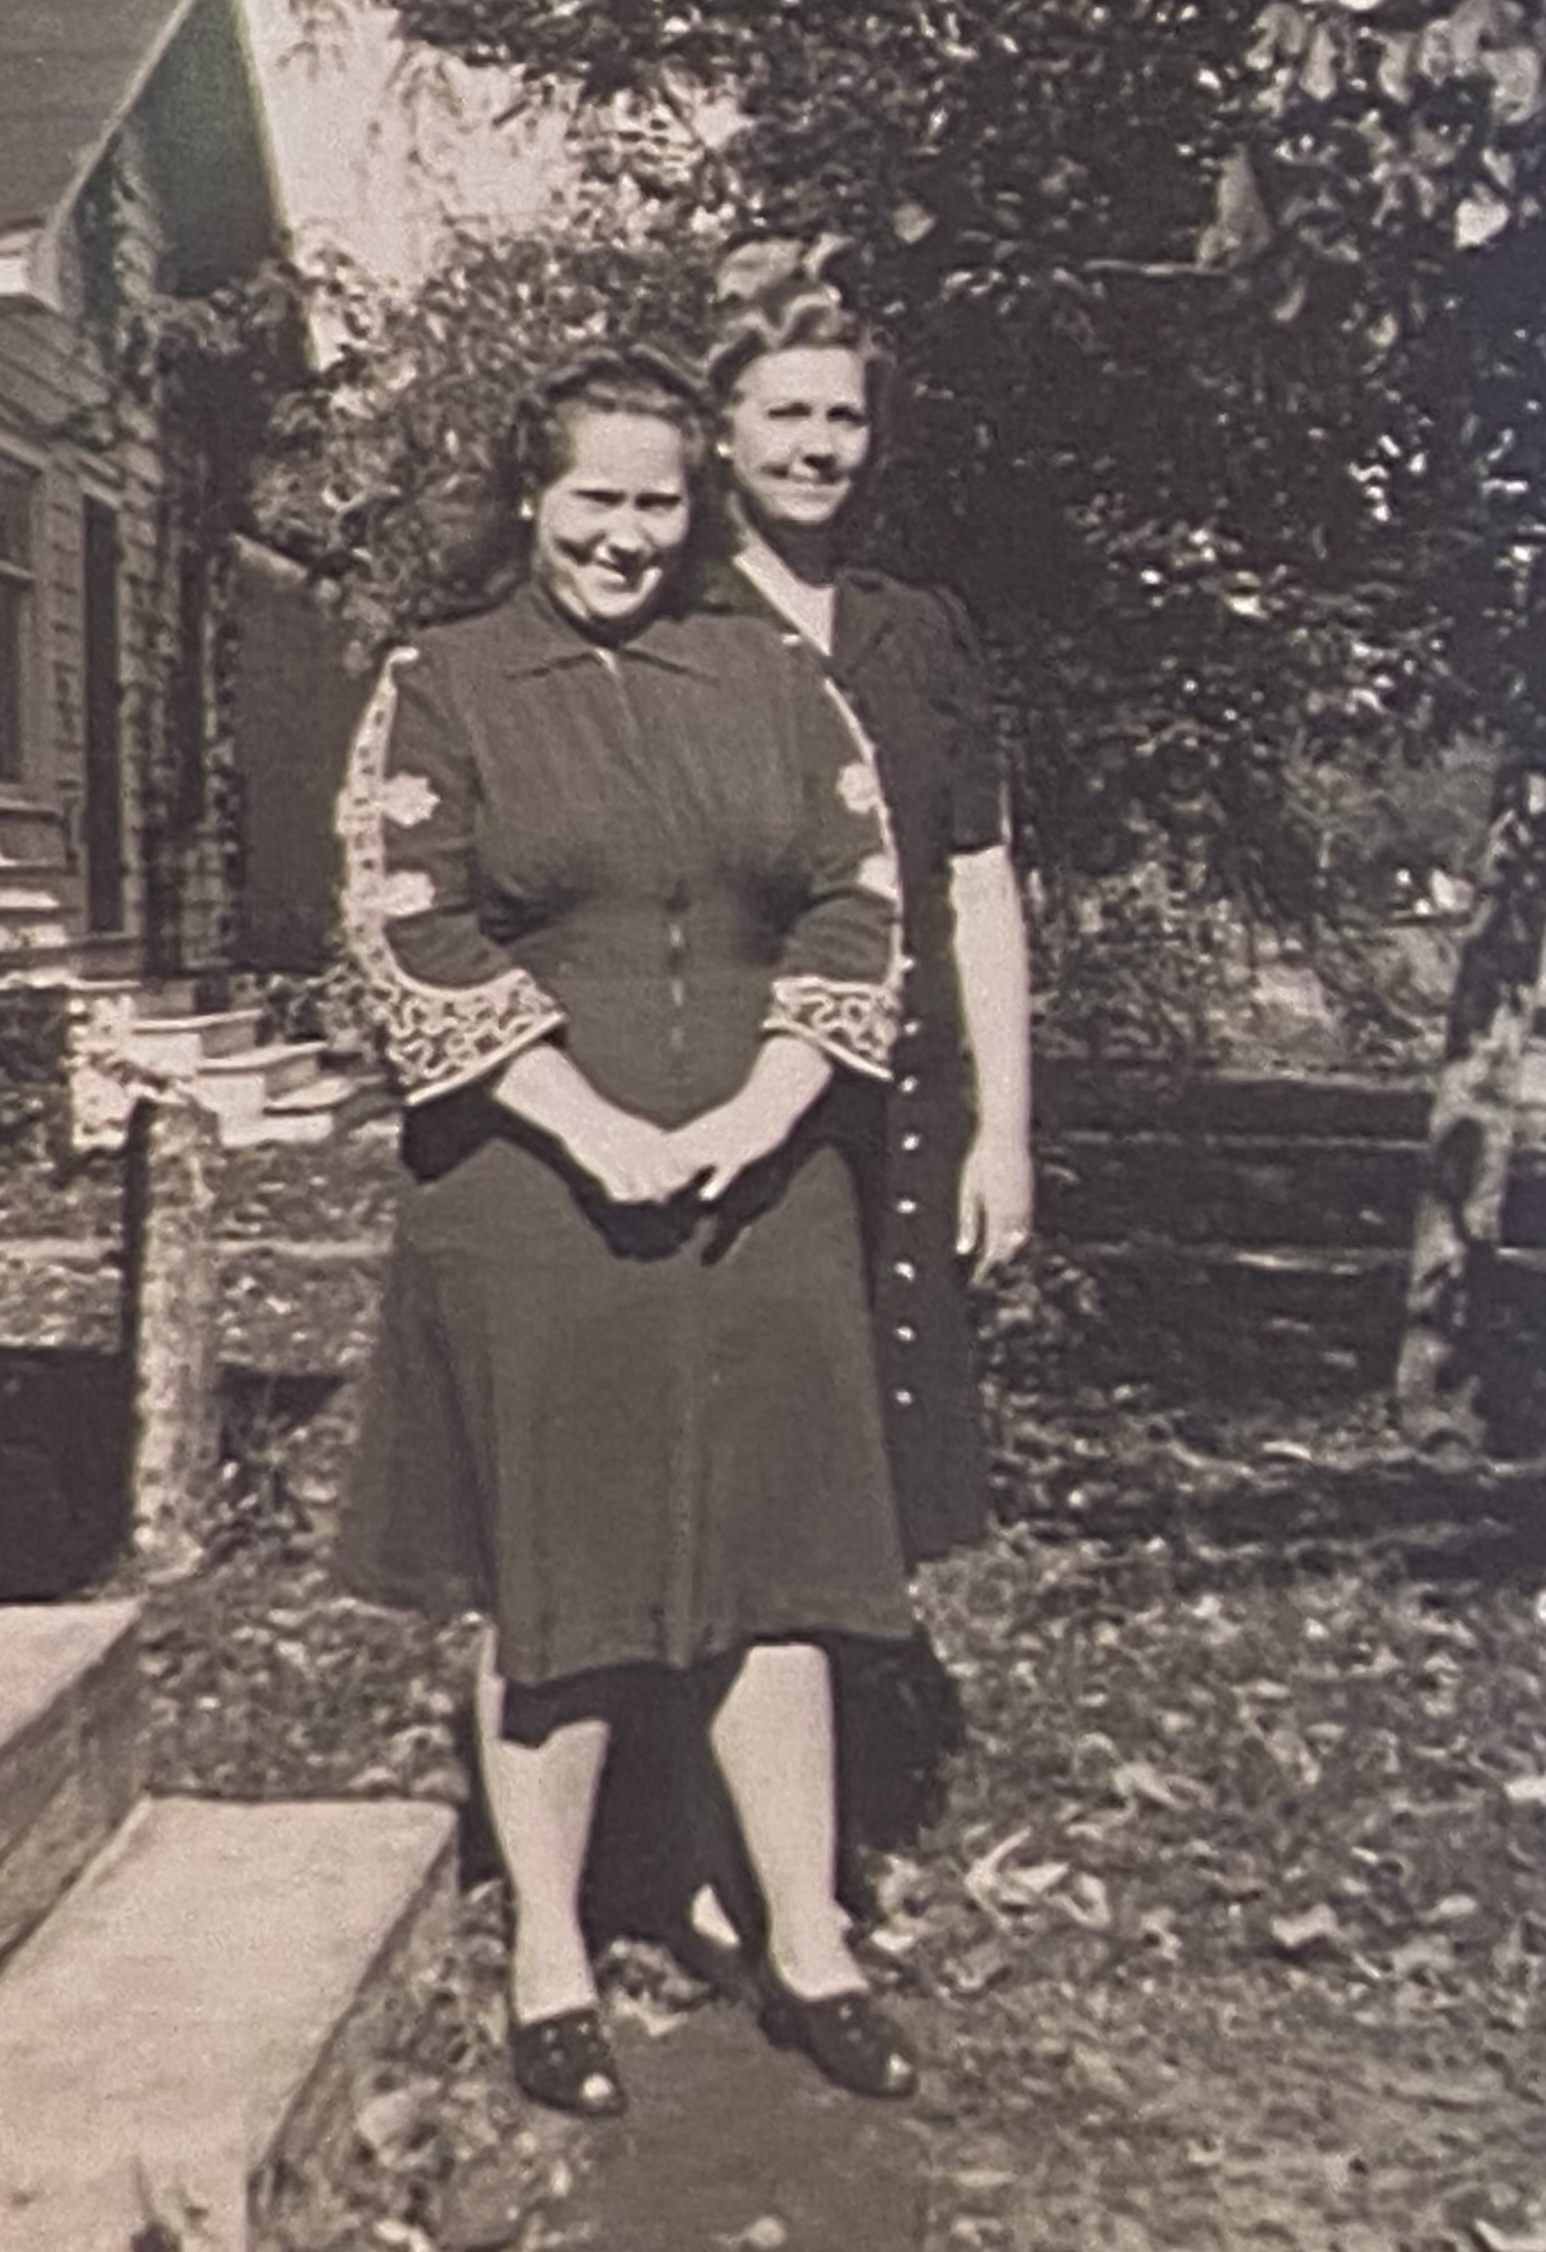
\includegraphics[width=0.55\linewidth,height=\textheight,keepaspectratio]{images/Akou22.JPG}

}

\caption[Lila (back) and Myrtle Schneider (front) circa 1946]{Lila
(back) and Myrtle Schneider (front) circa 1946; used by permission of
June Lewis}

\end{figure}%

\section{Notes}\label{notes-41}

I only have one sister, who is two years younger than me. As adults,
many of our conversations have been like this letter from Veda to
Lila---shallow and one-sided. Veda has good intentions and is
successfully building her own life, but she assumes that Lila has the
same goals. She is not very curious about the differences between them.

In this chapter, the Schneider family is destabilized when Herman's
mother has a stroke. The shocking news causes Lila to think about her
strained relationships with her sister and parents. When she visits
Myrtle in La Crosse, she gets even more shocking news---Viola and John
are getting a divorce. This was very unusual for a white, working-class
family in Wisconsin in the 1940s. Although both men and women could seek
a divorce, the state required them to publish the cause (such as ``cruel
and inhuman treatment'') in the local newspaper.

For more information, see Kristin Celello\footnote{\citeproc{ref-celello2009a}{\emph{Making
  Marriages Work: A History of Marriage and Divorce in the
  Twentieth-Century United States} (Chapel Hill: University of North
  Carolina Press, 2009)}.}, Joseph A. Ranney\footnote{\citeproc{ref-ranney1998a}{{``Traditional
  Values and No-Fault Divorce''} (Wisconsin Court System, 1998),
  \url{https://www.wicourts.gov/courts/history/article45.htm}}.}, and
Scott J. South and Stewart E. Tolnay, eds.\footnote{\citeproc{ref-south1992a}{\emph{The
  Changing American Family: Sociological and Demographic Perspectives}
  (Abingdon, UK: Taylor \& Francis, 1992)}.}

\bookmarksetup{startatroot}

\chapter{Chapter Forty}\label{chapter-forty}

Independence Day was on a Friday that year, so Nora and Gladys had
decided to hold a gathering in Veterans Park. It was close to the farm,
which would make it easy for Herman to drive back and forth. Lila had
never slept in a tent and wasn't sure what to expect, but she was
looking forward to spending some time with Myrtle and Gladys. It had
been a tough year. Alice was not getting better. Myrtle had lost the
baby. When Gladys asked Lila how she was feeling, she said,
``Exhausted,'' but when Myrtle and Carl arrived, she felt ashamed. Why
couldn't she just be satisfied with her life? At least the baby inside
of her was still alive.

When nightfall finally arrived, the men took the older children to the
riverside to shoot bottle rockets. Nora, Gladys, Lila, and Myrtle sat
around the fire. Nora's baby (her second and last) was just a few weeks
old. Gladys told them that Carl had proposed. It was wonderful news!
They tried to be lighthearted, but then the conversation took a dark
turn. They talked about Alice and Viola and John. Their children were
living with their grandparents in La Crosse until Viola could remarry.
Lila was surprised and said, ``Why?''

Myrtle had been lost in her thoughts, but she looked up and said, ``My
parents don't want them to be raised by a single mother. Viola should
have stayed with John.''

The conversation turned back to Gladys, but the news about the divorce
and Viola's forced separation from her children haunted Lila for months.
Would the Slabacks do the same to her if she left Herman?

On Saturday, Carl drove to La Crosse to pick up Helen. Her son, Duane,
was ten years old and growing fast. Wistfully Helen said, ``He's going
to be tall like his father.'' As they made lunch (grilled bratwurst and
blueberry streusel for dessert) she asked Lila if she had a place to
stay before the birth; if not, she could stay with her. Lila was
relieved. She had been thinking of asking Veda but wasn't sure that she
would agree. The contrast between Viola and Helen was striking. They
were both single mothers, but as far as she knew the Schneider family
was not pressuring Helen to marry again. Was it because she was widowed
and not divorced?

Herman drove Lila to La Crosse on the last weekend in July. Although her
last delivery had been at St.~Ann's, La Crosse Hospital was much closer
to Helen's house. Lila thought she knew what to expect, but she was
wrong. As soon as she arrived in the labor and delivery ward, the doctor
said he was going to ``medicate'' her. That was the last thing she
remembered. As soon as she woke up, she vomited. Once the bed was
cleaned up and she had regained her senses, the nurse explained that the
baby was turned sideways, so the doctor had put her under and given her
a ``c-section.'' Cheerfully, she added, ``Isn't it better than going
through labor?''

Lila was speechless. How was this better? The room was spinning, and it
hurt to cough. When they finally brought the baby into her room, she was
sleepy and difficult to feed. Was there something wrong with her? Lila
started to cry out of worry and frustration, and the nurse scolded her
for disturbing the rest of the mothers. She had never had surgery or
stitches before. The nurse who came to change her bandages every morning
would not allow her to touch her belly or see what the stitches looked
like. It was almost a week before they allowed Herman to visit his wife
and newborn daughter.

Lila was so disoriented from the birth that she didn't name the baby
right away. Herman suggested ``Alice'' after his mother. Alice was also
the middle name of Lyle's wife, Allene, so on the application for the
birth certificate she wrote, ``Alice Allene Schneider.'' As they drove
out to West Salem to pick up Myrtle Joyce and John, Lila wondered how
she was going to handle three small children along with the rest of the
chores. Myrtle Joyce had recently turned three, and John was not quite
two. It was daunting.

By the end of September, Lila felt like she was losing her mind. Her
life had become an endless stream of cooking and cleaning, snot, vomit,
dirty diapers, crying, and begging. Myrtle Joyce had responded to the
baby's arrival by refusing to take naps. John had learned to say NO and
MINE. Do you want a cookie? MINE. Share that with your sister. MINE.
Time for bed. NO. Herman was so good and patient with them. He loved the
children, and they loved him. She knew it wasn't a contest, but it made
her feel like a bad parent. Herman was busy with the cows and the
harvest, so most of the time it was just her and the children. They were
always getting into trouble with something: the stove, the pump, the
baby, the farm animals. Once she fell asleep from exhaustion and woke up
just in time to prevent John from falling through the hole in the
outhouse. That would have been a disaster.

One day, Lila was so desperate for relief that she piled the children in
the truck and drove to Veda's house. ``Why are they so dirty?'' Veda
asked. Myrtle Joyce and John were playing in the yard with David and
Patty. They were all laughing and throwing acorns, so they took the baby
inside to clean her up. When hot water came out of the tap, Lila started
crying over the ease of Veda's life. She suddenly realized that living
in a house with no running water was making her own life much more
difficult. Sternly, Veda said, ``You're the parent, Lila, not a child.
You need to pull yourself together.'' She left the bathroom to check on
the oven; they were having pot roast for dinner, cooked with an electric
oven. When she returned, she had clean outfits for the children. ``David
and Patty have outgrown these, so you can keep them.'' Mercifully, she
held Alice while Lila gave Myrtle Joyce and Johnny a bath. They didn't
fuss like usual; they were so fascinated by the indoor bath and the bar
of pink soap. Myrtle Joyce even let her wash and comb her hair. Lila
caught a glimpse of herself in the mirror, but it was like looking at a
stranger. There were dark circles under her eyes. Her hair was a mess,
and there was dried vomit on her shoulder; she had barely even noticed
when the baby spit up earlier that day. When dinner was done and it was
time to go, the younger children wailed, and Myrtle Joyce begged to stay
with her cousins.

When they got back to the house, Herman asked where they had been all
day. He wasn't angry, but Lila realized (with horror) that she had
forgotten to prepare something for dinner. He had been working hard and
deserved to have a hot meal. Lila said, ``I'm sorry\ldots I lost track
of the time. I'll cook you something right away.''

``That's alright,'' he replied. ``I'll have a peanut butter sandwich and
a glass of milk.''

The next day as she was making more bread, she decided that she would
ask Herman to put a lock on the door. If she could keep the older
children clean and safe indoors, maybe she could get a little bit of
sleep while Alice was napping.

\section{Notes}\label{notes-42}

When I was young, most of my family's vacations involved camping. I
enjoyed the freedom to go fishing and swimming and make new friends.
Myrtle Schneider and her second husband, John Schneider (Viola's former
husband) spent a lot of time camping in their RV at Veterans Park, so I
have vivid memories of camping there for family reunions.

This chapter offers more insights into attitudes surrounding divorce and
single parenthood in the 1940s, which could be---but were not
always---highly stigmatizing. Viola Schneider chose (or felt forced) to
send her daughters away until she could remarry. On the other hand,
Helen---a single mother due to her husband's untimely death---was not
forced to remarry quickly or give up her son. This chapter also
foreshadows that divorce is rattling in the back of Lila's mind as a
future possibility.

My mother, Alice, was Lila's third child. I know from newspaper
announcements that Lila's first hospital birth was at St.~Francis and
her second was at La Crosse Hospital. In the United States, the
medicalization of childbirth really accelerated in the 1940s. For the
first time, more children were born at hospitals than at home. While
this trend undoubtedly saved lives, it lengthened the time that mothers
spent away from their partners and younger children; it also increased
the rate of invasive procedures like cesarean deliveries.

When I was little, my mother usually purchased either Zest soap (which
was white) or Camay soap (which was light pink). I remember being
fascinated by the color of Camay. In the 1940s and 1950s, using
commercial bar soap in the bathroom was a solid marker of middle-class
life. In rural areas, it was still a luxury for many families.

For more information, see Lauren K. Hall\footnote{\citeproc{ref-hall2019a}{\emph{The
  Medicalization of Birth and Death} (Baltimore: Johns Hopkins
  University Press, 2019)}.}, Regina G. Kunzel\footnote{\citeproc{ref-kunzel1993a}{\emph{Fallen
  Women, Problem Girls: Unmarried Mothers and the Professionalization of
  Social Work, 1890--1945} (New Haven: Yale, 1993)}.}, Swasy\footnote{\citeproc{ref-swasy2012a}{\emph{Soap
  Opera}}.}, and Terence Young\footnote{\citeproc{ref-young2017a}{\emph{Heading
  Out: A History of American Camping} (Ithaca: Cornell University Press,
  2017)}.}.

\bookmarksetup{startatroot}

\chapter{Chapter Forty-One}\label{chapter-forty-one}

Winter started early that year. Myrtle Joyce was the first one to notice
the snow falling. ``What is that, Mom?'' The flakes were so small that
they were barely visible, but by November there was enough snow on the
ground to make a snowman. Just when Lila was starting to feel like she
couldn't take being a mother for one more day, the winter gave her
relief. Fall had been rainy and muddy; the colder temperatures froze the
ground. It was cold going to the outhouse, but it was easier to keep the
house clean now that they were no longer tracking mud all over the
floors. During her last trip to La Crosse, she had purchased coats and
boots for the two older children. Alice was already big enough to wear
Myrtle's coat from the year before. Evelyn had given her some handspun
yarn. Although Lila had not done any knitting for years, she managed to
make some basic scarves, hats, and mittens. They were ugly but warm.

Once the silage and hay were safely stored away for the long winter,
Herman had more time to spend at home. He started taking the children
out for walks---to climb on the bales of hay, to see what it was like in
the barn (Myrtle Joyce had been worried that the animals would freeze),
to see how the ice was forming on the creek, and to go sledding once
there was enough snow. He made snowshoes using strips of hide and wood
from an old barrel. Lila watched from the window as he taught the
children how to use them; it was funny to watch them tripping over their
own feet, but John was competitive with his older sister and determined
to be the first one to figure it out. The look on his face when he did
was pure delight.

Lila had stopped going to church after Alice was born. Herman went from
time to time, but the children couldn't go with dirty clothes. They
couldn't go if they had refused to eat that morning or if they didn't
get enough sleep the night before. They might cry in church, which would
be embarrassing to the whole family. Lila might have been able to manage
it with help, but with Alice needing so much support there was nothing
left for Gladys and Nora to give. It was heartbreaking to watch her
mother-in-law's decline. She could no longer hold or even talk with her
beloved grandchildren. Myrtle Joyce was too young to remember what she
was like before the stroke. During one visit, she asked, ``Who is that
scary woman in the corner?''

Lila was mortified. Gladys gently took Myrtle Joyce and Johnny by the
hand and said, ``Why don't we go play outside for a little while?''

The Schneiders were always kind, but remembering the incident made Lila
feel like she wanted to disappear.

Carl and Gladys married in December, but there was already too much snow
to drive the truck. Lila was sad to miss it. She had hoped they could
visit West Salem for Easter, which was at the end of March. The snow had
started to melt, but then there was a blizzard. ``In like a lamb, out
like a lion,'' said Herman as the children watched through the kitchen
window. Lila cooked a ham for the occasion, but it didn't feel like much
of a celebration. A week later, Alice died at home in West Salem.

That spring there was a new postman. He was younger than ``Rudolph'' and
had striking white-blonde hair. The first time he came to the house, he
smiled and said, ``I'm Fred Hicks and you\ldots must be very busy!''
Lila had taken the children outside for some fresh air, and they had
discovered the mud around the water pump. She took the letter (which had
Veda's handwriting) and dashed into the house without saying a word; by
the time she returned, he was already gone. A few days later, he
delivered a letter from Gladys. When Lila answered the door, she said
``Hi, I'm Lila.'' Replaying the moment in her mind that night, she
kicked herself for being so stupid. He knew her name already; it was on
the letters. Two weeks went by before Fred returned for another
delivery. Surprisingly, he said, ``Do you like jokes? I have a joke for
you.''

\begin{quote}
One Sunday at church, the pastor was giving a sermon about forgiving
your enemies. He said, ``Raise your hand if you can forgive your
enemies.'' Only half of the men and women raised their hands.
Undeterred, he kept speaking. After ten minutes, he asked the same
question. This time, three-quarters of the congregation raised their
hands. Another ten minutes went by, and he was really getting into it!
He asked the question again, and everyone raised their hands except for
one person.

``Mr.~Olson,'' he said with obvious frustration, ``Why are you so
unwilling to forgive your enemies? Surely, after living for eighty-six
years, you should be able to do this with ease!''

``I can forgive,'' replied Mr.~Olson, ``but at this point\ldots all my
enemies are dead!''
\end{quote}

The joke was not that funny, but Lila laughed. She had not heard a joke
in such a long time. It felt good to laugh again.

Fred's joke got her thinking about jokes she had heard from Lloyd and
from the soldiers. Many of them were not appropriate to tell around the
children, but by the time Fred returned she had thought of one that was
not too bad.

\begin{quote}
A man walks into a courthouse and tells the clerk that he wants to
change his name. The clerk is busy with filing, so he says impatiently,
``Alright, what is your current name?''

``Adolf Cockburn,'' the man replies.

In shock, the clerk stops filing. Feeling more sympathetic, he pulls a
form out of a drawer and says, ``What name would you prefer to have?''

With a smile, the man replies, ``James Cockburn.''
\end{quote}

Fred turned red in the face. Just when Lila thought that she had really
offended him, he started laughing so hard that he couldn't speak.

That spring, Alice and John started teething at the same time. A less
experienced mother might have thought it was just a cold, but John was
sucking him thumb again. Alice was starting to pull herself up and was
gnawing on the edges of the bed frame. They were feverish, cranky, and
hardly sleeping. Somehow, Myrtle Joyce was able to sleep through it, but
Lila and Herman were not. After a week of losing sleep, Herman said,
``We really need to slow down on having children.'' Lila agreed, but
when they were not intimate, she felt like he was slipping away; it was
the only way she felt truly connected to him.

It was calving season, and Herman was spending longer days in the barn.
She was never alone, but there were many times when she felt lonely. She
yearned for some real conversation with another adult. Even when they
were together, Herman still didn't talk much.

Fred and Lila continued trading jokes. One day he said, ``I'm allowed to
have some time off for lunch. Would you mind if I sat here and ate with
you?'' When Lila didn't respond right away, he added ``I don't mean to
impose\ldots I have a sandwich in my bag.''

Lila smiled and said, ``Sure, let me make you some coffee to go with
that.''

For several weeks they ate lunch together outside. The children enjoyed
having ``picnics'' with Fred. Myrtle was just big enough to help by
setting the plates on the blanket. It was something to do in the
mornings. And then one day, he arrived during a thunderstorm. Fred
knocked on the door to deliver the mail and said, ``I guess I better go.
It's too wet to eat outside today.''

Lila felt like her heart was falling into her stomach and quickly said,
``No, don't go\ldots you can come inside.''

The wind had picked up and it was rattling the windows. Alice was
giggling as her older brother jumped on the bed, but storms always made
Myrtle Joyce nervous. As soon as Lila was done making the coffee and sat
down at the table, Myrtle Joyce climbed into her lap. Fred didn't seem
to mind the chaos. He swallowed a bit of his sandwich and said,
``So\ldots you told me that you grew up in La Crosse. Where did you go
to school? What kinds of things did you do for fun?'' Herman was not
interested in the past or the future, only in the present. He had never
made Lila feel guilty for her bad choices, but he had also never asked
what her life was like before they got married. At times, his silence
felt uncaring. Being with Fred was different. It reminded her of being
with Lloyd. She told him about going to the movies for the first time to
see \emph{The Wizard of Oz}. He had never seen it. As she described the
film, he listened with rapt attention and laughed at her imitation of
the Wicked Witch.

Myrtle Joyce had fallen asleep in her lap. Fred said, ``I guess I should
get back to work now\ldots the mail won't deliver itself.'' Lila began
to push her chair back from the table, but he said, ``No need, I can let
myself out.'' He leaned over and kissed her on the forehead. It was so
quick and unexpected. Before she could say anything, he was halfway out
the door. She knew the kiss was wrong, but she wanted more of them.

\section{Notes}\label{notes-43}

This chapter draws from my own experiences growing up as a child in
northern Wisconsin. I remember how magical it was to see the first
snowfall of the year. When I was in elementary school, my mother knitted
scarves, hats, and mittens for me and my sister. (She was good at it,
but homemade clothing was not very ``cool'' in the 1980s.) I learned the
phrase, ``In like a lamb, out like a lion,'' in my first-grade
classroom.

I also remember visiting elderly relatives who lived in nursing homes.
My mother pointed out that they were so happy to see me (a child), but I
was unsettled by their stares and touches.

Lila is still struggling with living on the farm, especially with three
small children. She is more isolated than ever from other adults; this
is a common experience for young mothers. I have no idea what her
relationship was like with my grandfather, but I imagine the hard work
of raising small children was draining on their marriage. She may have
been looking for a way out. This chapter reminds us of her sense of
humor.

Rural mail delivery was not guaranteed by the U.S. Postal Service until
1902. Even then, rural mail carriers were allowed certain flexibilities
that urban carriers were not.

For more information, see Winifred Gallagher\footnote{\citeproc{ref-gallagher2016a}{\emph{How
  the Post Office Created America: A History} (New York: Penguin
  Publishing, 2016)}.}, Chelsia Harris\footnote{\citeproc{ref-harris2018a}{\emph{Hannah
  Visits Nana in the Nursing Home} (Meadville: Christian Faith
  Publishing, 2018)}.}, and Esther Perel\footnote{\citeproc{ref-perel2017a}{\emph{The
  State of Affairs: Rethinking Infidelity} (New York: HarperCollins
  Publishers, 2017)}.}.

\bookmarksetup{startatroot}

\chapter{Chapter Forty-Two}\label{chapter-forty-two}

Lila wasn't trying to push Herman away. If someone had asked her why she
let Fred into the house, she would have said that she was just being
polite. He needed a place to eat lunch, so why not? It was nice to have
a conversation with another adult.

\begin{figure}[H]

{\centering 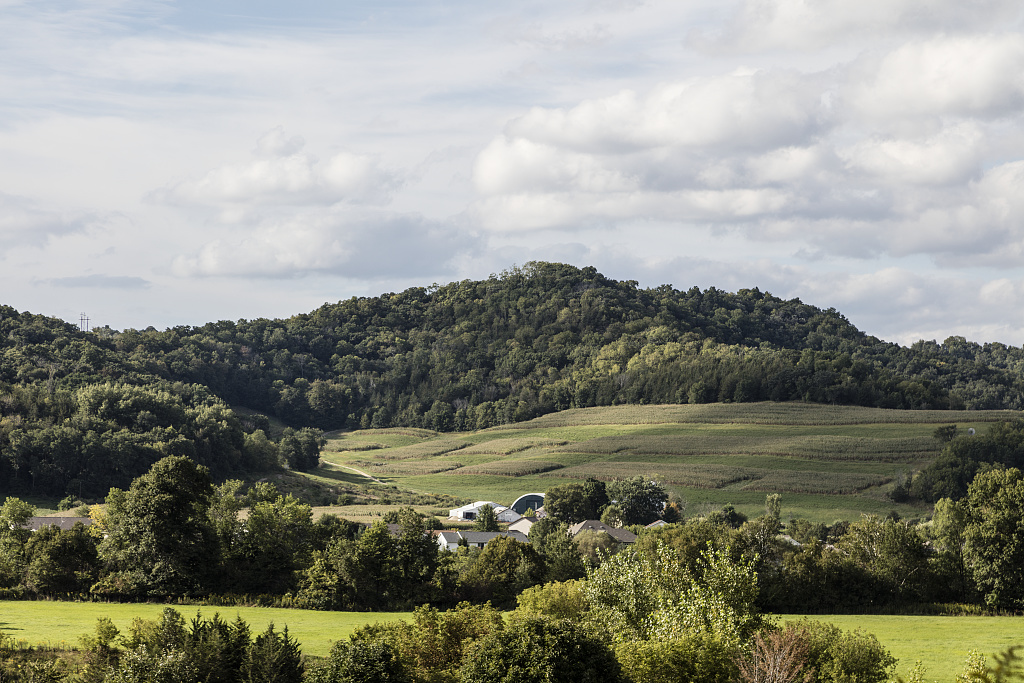
\includegraphics[width=0.85\linewidth,height=\textheight,keepaspectratio]{images/Akou23.jpg}

}

\caption[Farmland and bluffs in La Crosse County, Wisconsin]{Farmland
and bluffs in La Crosse County, Wisconsin; Library of Congress Prints
and Photographs Division, \# LC-DIG-highsm-40479}

\end{figure}%

Many of the houses in that area were set close to the woods. It was very
hilly, so the flat parts needed to be reserved for the fields, which
were mostly for corn, oats, and hay. Vilas and Evelyn's house was at the
edge of their largest field, but the little house where Lila and Herman
lived was tucked into the edge of the bluff. Although the front yard got
plenty of sun, the back yard was always in the shade and the ground was
covered with a thick layer of fallen oak leaves and pine needles. It
attracted mice and snakes, so Lila preferred to stay in the front.

One day when Fred arrived for lunch, they were still inside the house.
The children were playing with a kitten that Herman had rescued from the
barn. Fred said, ``Could you come with me for a second? There's
something I want to show you.'' Lila followed him to the back of the
house, thinking he had seen a snake or maybe a deer. Instead, he cradled
her head in his hands and passionately kissed her on the mouth. After a
few moments, he let go and said, ``I've been wanting to do that for so
long.''

With a whisper, Lila replied, ``Don't stop.''

Fred put his arms around her, and they leaned against the house, quietly
making love.

It was challenging to find time alone. Lila constantly worried that
Herman would come home or the children would see them, but she craved
being with Fred. It felt so good to be in his embrace. He said the most
gentle and loving things. ``You're such a beautiful woman, Lila.'' ``I
love being with you.'' She knew that it was wrong to have an affair with
a man who was not her husband, yet she couldn't help wanting to be
together. Lila loved the Schneider family and felt a deep sense of love
and acceptance that was lacking from her own family, but as Veda had
predicted, she was not a good match with her husband. Fred was closer to
her age, and they could talk with an ease that she and Herman had never
achieved.

One day when he finished eating lunch he said, ``Would you like to hear
a song?''

Myrtle Joyce clapped her hands and said, ``Yes, a song!''

He laughed and started singing:

\begin{quote}
My young love said to me, ``My mother won't mind,\\
and my father won't slight you for your lack of kind.''\\
Then she slipped away from me, and this she did say\\
``It will not be long, love, 'till our wedding day.''
\end{quote}

Lila had not heard any music for months. Fred's voice was breathtaking,
but the song sent chills up her spine. The ``young love'' turned out to
be a ghost calling for her love to join her. ``Where did you learn
that?'' she gasped.

He grinned and said, ``My mother is Irish. I think she learned it as a
child. Did you like it?''

Johnny chimed in with his sweet little voice and said, ``More!''

The next song was more upbeat, but it was also about two lovers.

\begin{quote}
Come won't you walk with me, Griselda,\\
wearing the dress that moonlight shines through.\\
I am a sad and lonely boy,\\
since your mother said I couldn't see you.\\
\strut \\
Slip into the woods in the dark of the night,\\
Call to the moon out yonder:\\
Oh, lady moon, won't you shine a silver light\\
and lead me to my Griselda.
\end{quote}

Lila blushed. What if someone heard what he was singing? He was
practically advertising their love affair. Lila turned to look for
Alice, and there was Herman, standing at the edge of the front yard.
Fred stood up from where he had been sitting and said, ``You must be
Mr.~Schneider.'' He held out his hand, but Herman refused to shake it.
``I guess I better be going now,'' he said with a strained cheerfulness.
Herman's face was darker than usual. He stared at Fred as he walked down
the path. When he was out of sight, Herman said, ``I'll be back for
dinner.''

The tension was thick that night in the house. Lila was not hungry, and
the children were unusually quiet. When he finished eating, Herman said,
``Fred Hicks will not be coming back to this house. If you want to mail
a letter, give it to Evelyn.'' Lila's heart was thumping hard in her
chest. How much did Herman know? Did Evelyn tell him something? When
they went to bed, Herman slept facing the wall. He didn't raise his
voice or make any other demands, but he was clearly angry. For weeks he
said almost nothing. On the outside, Lila was calm. On the inside, she
was screaming, ``Yes, I had an affair! Say something about it! Get
angry! Was it so wrong wanting to be held and loved?'' Lila wanted to be
more than just a mother and a housewife. For a brief time, she had that
with Fred. Now he was gone, and the silence was deafening.

\section{Notes}\label{notes-44}

When I was in college, I performed with a student-led folk music group.
Many Irish ballads are about romance, drinking, and/or war; the songs I
quoted from are two of my favorites. Although I found the name ``Fred
Hicks'' in the 1940 census for West Salem (he was the right age for this
character), I have no idea if he worked as a postal carrier or ever met
Lila. ``An affair with the mailman'' is a classic trope, but it could
have been true in this case.

I married a little earlier than Lila, just before I turned 21. I wish I
had spent more time thinking about my upbringing and what I might want
as a mother. My hopes and expectations for family life turned out to be
very different from my husband's. I never had an affair, but I
understand why some people do. Like my grandfather, I found my (now
former) husband difficult to know and connect with.

For more information, see Jerry Apps\footnote{\citeproc{ref-apps2006a}{\emph{When
  Chores Were Done: Boyhood Stories} (St. Paul: MBI Publishing Company,
  2006)}.}, Peter Kennedy\footnote{\citeproc{ref-kennedy1984a}{\emph{Folksongs
  of Britain and Ireland} (San Francisco: Oak Publications, 1984)}.},
and Alvin Martin Peterson\footnote{\citeproc{ref-peterson1948a}{\emph{Palisades
  and Coulees: The Scenic Mississippi Valley from Prairie Du Chien to
  Red Wing} (Onalaska: Modern Print Company, 1948)}.}.

\bookmarksetup{startatroot}

\chapter{Chapter Forty-Three}\label{chapter-forty-three}

When Lila moved to West Salem, she had more than three hundred dollars
in small bills stashed away from working. She had used some of it to
purchase her wedding dress. Since the wedding, she had used a trickle of
the money to stretch the household budget. Stationery and postage
stamps. Her driver's license. A new pair of boots for Johnny after he
lost one playing outside. (They never did find it.) A bit of lace to
make a pretty dress that Myrtle Joyce could wear to church. Two pounds
of coffee for the picnics. Nothing extravagant. Herman never said a word
about it; she wasn't sure that he even noticed. By the time her affair
with Fred Hicks was over, the stash was small enough to fit into an
empty can of baking powder.

Lila had fantasized many times about leaving the farm, but as the days
of silence turned into weeks, her fantasies became more urgent. Should
she take the truck and just drive to La Crosse? Would Herman follow her?
Did she want him to? Where would she live? Should she take the children
along? For a few days, she seriously considered just walking
away---taking a train and getting out of Wisconsin, starting a whole new
life. It was an appealing thought. She was only twenty-six years old.
But then doubts crept in. What would happen to their children? Who would
raise them? Would she miss spending time with the Schneiders? Would she
miss Veda or the rest of the Slabacks or even just La Crosse? She felt
like she was standing on the edge of a powerful river; she could get in
and let the current carry her away to an unknown destination, or she
could turn and walk back to solid land. Stay on the farm or move to La
Crosse. Stay with the Schneiders or go back to Veda. For days, she
wracked her brain for other options. She fantasized about standing on
the bridge to French Island, steeling herself to jump into the river. It
was such a dark fantasy that it made her shudder. She forced the thought
out of her mind; it was a sin to think about ending your life. The
children needed her. If she was gone, where on earth would Herman find
another wife to take care of them?

Lila was waiting for some kind of sign that it was time to decide.
August was hot and dry, but in early September the weather suddenly
turned gloomy. After several days of rain, Lila woke up to see a
brilliant beam of light piercing the clouds. The light poured through
the bedroom window and filled her with a sense of strength and purpose.
It was the sign she had been waiting for---the day to take the next
step. Herman had left to do the milking, so she went to the pump to draw
a bucket of water. By the time she was heating the water on the stove to
make coffee and give everyone a quick wash, she was humming a song that
she remembered from long ago on the radio.

They couldn't take much without arousing suspicion. It had to look like
they were just leaving for the day to visit La Crosse. Lila filled a
small bag with a change of clothes and some diapers for the baby. She
put her hairbrush, a packet of letters, and the baking powder can of
money in her purse. As they walked out the door, Myrtle Joyce sobbed,
``We can't leave Kitty!''

Her sense of panic almost made Lila turn back. Gathering her composure,
she knelt and said, ``Don't worry, Kitty will be fine. You'll see her
again later.''

Johnny was more excited. When they got into the truck he said, ``Go,
mommy!''

``Well, alright then,'' she replied as she pushed the button to start
the truck's engine.

Lila knew that there was a train station in West Salem. She had decided
that she would drive to the station, buy tickets to La Crosse, and leave
the truck there. Somebody would figure out who the truck belonged to and
let Herman know. What would happen next? Would he just go back home?
Would he drive to La Crosse to look for her? She wasn't sure what she
wanted him to do. She just knew that something had to change. Veda and
Red's house was only three blocks away from the train station in La
Crosse. When the train arrived, they would walk from the station to
Veda's house and then she would figure out her next move.

When Veda opened the door, she said, ``Oh, Lila. I wasn't expecting you.
Come on in.'' Myrtle Joyce and Johnny darted into the house to look for
their cousins. ``David is still at school, but the bus will drop him off
in a couple of hours. I was just getting ready to make lunch.''

Lila stepped inside and said, ``I can help if you like.''

Veda tilted her head to the side. Did she suspect that something was
wrong? She straightened back up and smiled faintly. ``It's kind of you
to offer, but I can handle it. Have a seat.''

Lila put Alice on the floor. She had just started walking and
immediately pulled herself up on the sofa. Lila took off her sweater and
put it in the diaper bag. In the corner there was a new television set.
Lila had never seen one before. At first, she thought it was a radio.
Veda returned to the living room and saw her staring at it. ``We got
that a couple of months ago. Sometimes we make popcorn and invite the
neighbors over to watch with us like our house is a miniature movie
theater.''

``Oh, that's nice,'' said Lila. She suddenly felt like she had taken
more than just a trip to La Crosse; she had stumbled into a new century.

After lunch, Veda made tea. ``I looked out the window, but I didn't see
the truck. Did Herman drop you off?''

Lila hesitated. Now the truth was going to come out, ready or not. ``No,
we took the train this time.''

``Oh?'' said Veda. ``Are you planning to stay for dinner?''

``If that's alright with you,'' Lila replied. She took a sip of the tea.
It was hot and burned the roof of her mouth.

``Yes, of course that's fine.'' Veda put her hand out. ``Lila\ldots is
everything alright?''

Lila was starting to sweat. ``Um\ldots well, you see\ldots we're moving
to La Crosse. Just me and the children\ldots without Herman.''

Veda's mouth fell open in shock. ``What happened? Did he hit you?''

``No, nothing like that,'' said Lila.

``Then what? Did he have an affair?'' Veda had set down her cup of tea
and her eyes were open wide.

Lila's stomach twisted into a knot. For a few seconds she was silent.
They could hear the children running around and laughing upstairs.
Quietly, Lila said, ``I just couldn't keep living there.''

Veda stared at her. ``I don't understand. Herman is your husband. You
can't leave him for no reason.''

Lila looked down into her lap. Had she been wrong to leave? How was she
going to explain this? Summoning her last bit of courage, she looked at
Veda and said, ``Could we stay here for a few nights? I can find a job
and a place to live\ldots it won't be for long.''

Veda's lips were tightly pinched. She looked both angry and concerned.
``The children can stay here for a few nights. You need to take the
train back to West Salem and straighten this out right away.''

Suddenly they heard footsteps on the front porch. It was David,
returning from school. By the time the door opened, Veda had flipped to
``loving mother.'' ``How was your day, dear?''

``It was good, Mom,'' said David. Before Veda could say anything more,
he turned and said, ``Hi, Aunt Lila.''

Lila raised her hand to say hello, but he was already heading upstairs
to look for his cousins. When he was out of earshot, Veda turned back to
Lila. ``You should leave now. I don't know what you need to do to make
this right, but your children will be fine. Just go.''

Lila picked up her purse. Without saying another word or looking back,
she went out the door, down the steps, and started walking back to the
train station. Her mind was blank. In the distance she could hear a
whistle; a train was coming into the station. Should she buy a ticket
and go back to West Salem? Instead of going to the ticket window, she
decided to sit on one of the benches by the tracks. A train was getting
ready to leave. An agent in a dark blue suit leaned out of one of the
middle doors and said, ``Last call for Rochester with service to
Winona.'' Where would the train go after that? She sat on the bench for
what felt like hours, watching the trains. Eventually, someone came out
of the station to ask, ``Ma'am, are you alright?''

``Yes, I'm fine, thank you. I was waiting for someone, but it appears
that they're not going to show today.'' She was astonished at how easily
the lie tumbled out. She stood up and started walking in the other
direction, away from Veda's house and toward the river.

By then it was late afternoon. It was getting chilly, and the sun was
low on the horizon. Maybe the children were eating dinner. Without even
thinking about where she was going, she had reached Copeland Park. She
walked past the playground---there were only a few children playing on
the swings and the merry-go-round---and headed right down to the river.
In a few minutes, she could see the Clinton Street bridge. Her darkest
fantasy was coming to life.

As she walked closer, she thought about an accident that had happened
when she was a child. This bridge could only handle small cars, but
there was a larger bridge on the south side of La Crosse. One day, a man
driving a car passed out as he was crossing and collided with one of the
support beams. It caused a big section of the bridge to collapse and
fall into the water, and his car fell with it. He managed to get out and
swim to safety, but two of his passengers drowned. Lila heard the story
at the dinner table; one of her brothers (maybe Lyle) had read the
newspaper article out loud. It gave her nightmares for months. The
crash. Plunging into the river. Drowning while trapped in the back seat.
Lila had walked over the replacement bridge many times, but she never
really trusted it. The water below was always dark and churning.

Lila sat on a boulder near the pilings. How long did she stare at the
river? Her body was numb with the cold. The moon was nearly full. She
could see its swirling reflection in the water. Subconsciously, she had
hoped that a brilliant solution to her problems would spring to mind,
but nothing came. Her mind was as numb as her body. She could hear cars
going back and forth over the bridge, but nobody walked by. She was
completely alone.

Eventually, the sun crawled back over the horizon. With a sigh, she
climbed up the bank and crossed over the bridge to French Island.
Everything looked golden in the early morning light. She caught a
glimpse of herself in a window. Her dress was dirty and wrinkled and her
hair was a mess. She laughed out loud thinking, ``I look like a
banshee.'' Then she sat on the curb and her laughter turned into sobs.

\section{Notes}\label{notes-45}

For many couples, the household budget is a major challenge. It was for
me. I often spent my own money on things for the kids and the house that
I'm sure my husband never noticed. Money is a significant barrier for
many women who want to leave a marriage. Many occupations (and the tax
codes) are structured to benefit heterosexual, married couples and
punish singles. Until the Equal Credit Opportunity Act was passed in
1974, women were not allowed to open a bank account without a male
co-signer.

This chapter is a pivotal moment in the book. Lila has decided to walk
away from her life with Herman. She doesn't really know what she wants;
she only knows what she doesn't want. She takes a leap of faith into the
unknown, but will she have the courage to stay there?

For more information, see Thomas Joiner\footnote{\citeproc{ref-joiner2009a}{\emph{Why
  People Die by Suicide} (Cambridge: Harvard University Press, 2009)}.},
Peg A. Lamphier and Rosanne Welch, eds.\footnote{\citeproc{ref-lamphier2017a}{\emph{Women
  in American History: A Social, Political, and Cultural Encyclopedia
  and Document Collection} (Oxford: Bloomsbury, 2017)}.}, Lynn
Spigel\footnote{\citeproc{ref-spigel1992a}{\emph{Make Room for TV:
  Television and the Family Ideal in Postwar America} (University of
  Chicago Press, 1992)}.}, and Evan Stark\footnote{\citeproc{ref-stark2009a}{\emph{Coercive
  Control: The Entrapment of Women in Personal Life} (Oxford University
  Press, 2009)}.}.

\bookmarksetup{startatroot}

\chapter{Chapter Forty-Four}\label{chapter-forty-four}

An older woman tapped Lila on the shoulder. ``Are you alright, dear?''
Lila looked up, and a tear dripped off the end of her nose. ``Why don't
you come with me? My house is just a few blocks away\ldots you look like
you could use a cup of coffee.''

The woman introduced herself as Emma as they walked to her house. It was
extremely small, but the kitchen was cozy and warm. Emma took a frying
pan off the shelf and set it on the stove. ``How do you like your eggs,
dear?''

Lila took a seat at the table. ``Oh\ldots fried, I guess?''

With a warm smile, Emma replied, ``Fried eggs and toast, coming right
up.''

Lila's stomach rumbled. Her last meal had been lunch at Veda's house. It
was very quiet. For a few minutes, they listened to the sound of the
eggs frying and a train whistle blowing in the distance.

Lila was the one who broke the silence. ``Do you live here by
yourself?''

``Oh no,'' chuckled Emma. ``The girls are married now, but my husband,
Edward, is at work and the boys are at school.''

``How many children do you have?'' said Lila.

``Three girls and three boys. The oldest, Margaret, is probably the same
age as you.''

Quietly, Lila said, ``I have three children. Myrtle Joyce, John, and
Alice.''

``Oh, that's lovely,'' said Emma. ``Children are such a gift.''

As Lila finished eating, Emma put her hand on Lila's arm and said very
gently, ``You seem to be having some trouble, dear. Is there anything I
can do to help?''

Lila's eyes welled with tears, and Emma offered her a handkerchief. When
her throat stopped clenching, she said, ``I don't know\ldots I guess the
first thing I need to do is find a job.'' She was staring at a smear of
egg yolk left on her plate.

Lila expected Emma to start asking questions and making demands, but
Emma just said, ``Well, now that your belly is full, let's get you
cleaned up. I think I have a dress you can borrow. I'll wash the one
you're wearing, and you can pick it up when you come back. Emma put a
pail of water on the stove and showed her to a room with a sink and a
mirror.''You can change your clothes here. I'll bring you soap and a
washcloth as soon as the water is ready.'' Lila had a comb in her purse
and started fixing her hair, avoiding her reflection in the mirror. The
dress from Emma was not stylish, but it was clean. By the time she had
washed up, the sun was bright overhead. Emma gave her a hug, and Lila
walked back in the direction of the bridge. She had noticed that there
was a new tavern on Bainbridge Street.

When Lila pushed open the door, there were just a few locals sitting at
the bar for lunch. It was dark and there was already a cloud of smoke in
the air. She immediately wanted to leave, but the bartender said, ``Is
there something you need?''

Swallowing, she replied, ``I'm looking for a job as a cocktail
waitress\ldots I worked at Carroll's during the war.''

The bartender looked her up and down in a way that made her skin crawl.
``Is that so? I might have a job for you if you come back tonight.'' One
of the men at the bar laughed. Without saying another word, she turned
and left. She might be desperate, but not that desperate.

Carroll's was only two blocks away, but Lila resisted going in. She
worried there would be nobody left who remembered her; worse, that
somebody would remember exactly why and how she had left. Summoning her
last bit of courage, she walked into the supper club across the street
from Carroll's. She had never been inside before. The restaurant was on
the edge of the water, and the entire back wall was filled with
windows\ldots the view of the water was impressive.

``Would you like a seat at the bar?''

Lila snapped back to attention and said, ``Actually, I came to see if
you were hiring.''

The hostess was older than Lila, but well put together. She was wearing
a pearl necklace and a black dress with a sharply tailored white collar.
She said, ``I'll take you to the kitchen, so you can talk with the
owner. I'm his wife, Stella.'' To Lila's relief, he asked how quickly
she could start working.

When Lila returned to Emma's house, her sons were home from school. She
hugged Lila like they were old friends and invited her to stay for
dinner.

``That's so kind of you, but now that I've found a place to work, I need
to find a place to live.''

``You can stay here for one night,'' Emma said. ``Why don't you look for
a place to live tomorrow when you've had some rest?''

She had a point. Lila felt tears welling up again, but Emma put her hand
on her shoulder and said, ``It's no trouble, dear. Whatever problems
you're having will work themselves out.'' Lila fell asleep on her sofa
not long after dinner, and Emma covered her with a quilt. She slept
heavily without dreaming.

She left Emma's house early the next day, hoping to find an apartment
and buy some new clothing before starting her shift at 4:00 p.m. It was
easier than she had expected to find a place to live. It wasn't much,
but she could afford the deposit of one hundred dollars. It was on Rose
Street, not far from the boarding house where Lloyd had lived. The rent
included water, heat, and electricity. The restaurant did not require
uniforms, but Lila realized that she would need to be more stylish if
she was going to work her way up from washing dishes to being a waitress
again. She purchased a long, gray skirt, two white blouses, and a cheap
pair of black pumps that caused terrible blisters until she could afford
to replace them.

Her next goal was to bring the children back to the apartment, but when
she went to pick them up, Veda asked sternly, ``Who exactly is going to
watch them while you're working?'' Lila had hoped that Veda might offer
to help. It was crushing to leave her house (alone) for a second time.
As she walked out the door, Johnny screamed ``Mommy\ldots Mommy, don't
go!''

Emma had invited her back for dinner that week. Lila offered her two
dollars, but she refused to take it. ``You're going to need that for
your children, dear.'' As they worked together on preparing the meal,
Lila decided to ask Emma for advice. It felt strange; she had been able
to confide in Lloyd, but his problems were always so much worse than
hers. Lila worried that she was asking too much.

Emma turned from the stove and said, ``You could put an ad in the paper
for a childminder, but why don't you bring the children here while
you're working?''

``Really?'' said Lila. She could hardly believe the depth of Emma's
kindness. ``That would be so helpful, and the restaurant is nearby.''

``That settles it then,'' said Emma. I'll cover the first two weeks.
After that, you can hire someone, or pay me whatever you think is
fair.''

\section{Notes}\label{notes-46}

When I reconnected with one of my mom's sisters in early 2020 (just
before the pandemic), I was astonished to learn that Emma was the
children's babysitter. I have no idea how she and Lila met, but I have
such fond memories of visiting Emma at her little house on French
Island. She was an incredibly kind and gentle person. If anyone could
have saved Lila from herself, it would have been Emma.

In my research for this book, I learned that Emma had a difficult
childhood. Her father was forty years older than her mother; Emma was
born when her mother was sixteen years old. Her parents had two more
children (both girls), but the second one died when she was only two
years old. Emma met her first husband as a teenager when she was working
as a servant on his parents' farm. I imagine these hardships are what
made her able to help Lila without judging her.

I was heavily pregnant when my firstborn child was two years old (nearly
three). She had been co-sleeping with me, but I decided that I needed to
make room for the new baby. So, one night, I tucked her into bed in her
bedroom (which she had never slept in) and closed the door to her room.
For an hour she cried and banged on the door with her tiny fists,
screaming, ``Mommy, my best friend, Mommy!'' It was heartbreaking. I
recalled that memory as I imagined Lila having to say goodbye to her
children for a second time.

For more information, see Gary Alan Fine\footnote{\citeproc{ref-fine2008a}{\emph{Kitchens:
  The Culture of Restaurant Work} (Berkeley: University of California
  Press, 2008)}.}, Greta Foff Paules\footnote{\citeproc{ref-paules1991a}{\emph{Dishing
  It Out: Power and Resistance Among Waitresses in a New Jersey
  Restaurant} (Philadelphia: Temple University Press, 1991)}.}, and
Valerie Polakow\footnote{\citeproc{ref-polakow1994a}{\emph{Lives on the
  Edge: Single Mothers and Their Children in the Other America}
  (University of Chicago Press, 1994)}.}.

\bookmarksetup{startatroot}

\chapter{Chapter Forty-Five}\label{chapter-forty-five}

Cleaning did not pay as much as being a cocktail waitress, but it was
just enough. Myrtle Joyce had started school, so on weekdays Lila
arranged to work from 4:00 to 11:00 p.m. It was brutal walking home from
Emma's house late at night (especially with Alice getting so big and
heavy), but the children loved her. Lila decided not to advertise in the
newspaper. The first three months in La Crosse felt like a dream. Lila
was making her own money and choices. Although she had not made a
conscious decision to hide, her life was simpler without the Slabacks
and the Schneiders; they had no idea where she was living.

In mid-November, the bars and restaurants on French Island started
putting up lights for Christmas. It gave the long nights a more festive
and hopeful feeling. There were not as many soldiers at Camp McCoy now
that the war was over, but there were still some; Carroll's was as busy
as ever, especially on the weekends. One night, a soldier noticed Lila
as she was leaving work and whistled to her from across the street.
``Hey there, gorgeous! Why don't you come over here for a minute?''
Against her better judgment, she walked across the street.

There were three soldiers standing together in the parking lot, smoking
cigarettes. Lila asked where they were from, and they offered her a
cigarette, but when she turned to leave, one of them grabbed her by the
wrist and whispered into her ear, ``The fun is just getting started.''
He pulled her into a dark corner between the building and the dumpster,
and one of the men put his hand over her mouth. ``Just be quiet and this
will be quick.'' She tried to get away, but they were too strong. While
two of the men held her arms and legs against the wall, the other one
raped her. Then they switched places. The struggle and the rough texture
of the bricks ripped her coat in the back. The last one grabbed her hair
and pushed her lower to the ground so he could force himself into her
mouth. She tried to bite him, but one of them slapped her so hard that
she nearly blacked out. How long was she trapped there? In her memories,
it would seem like an eternity, but it must have been only a few
minutes. It was the most violent thing she had ever experienced.

As she walked to Emma's house after the attack, Lila was shaking. Emma
noticed the rip, her messy hair, and the wet spots where her knees had
touched her skirt, but Lila brushed her off. ``It's fine\ldots I'm just
cold and tired. I'll be fine once I get the children home.'' It was
snowing as they passed Carroll's. The soldiers were gone, but Lila urged
the children to walk faster. When they got home, she tucked them into
bed and said, ``I'll be back in a few minutes.'' She locked herself in
the bathroom and wept silently for hours, hoping the children would not
notice.

For a few weeks Lila managed to perform most of her usual routine:
taking Myrtle Joyce to school, work, Emma's house, cleaning, feeding the
children, and putting them to bed at night. But for her, sleep was
elusive. Even when she fell asleep (which was not guaranteed), she often
woke up in the middle of the night in a sweat with her heart racing. By
early February, she was living in a constant fog.

One day when she dropped the children off at Emma's house Emma said,
``You look so tired, dear. Why don't you take a day or two off from
work?''

Lila looked down at her shoes. ``I can't really afford to.''

Emma hugged her, and she felt so solid and warm. Lila reluctantly let go
and waved goodbye to the children, who were looking out the front
window.

At the supper club, Lila had begun to work part of the time as a
waitress. She found that her memory was not as sharp as it used to be.
Even though she was writing the orders down, she sometimes forgot the
extra little requests that customers made (``Could you bring me another
cup of salad dressing, please?''). It was embarrassing. One day, the
owner's wife asked if they could talk for a minute after the dinner
rush. Lila said, ``Sure, no problem,'' but her heart sank.

Stella had grown her hair long and was pulling it back into a new style
that she called a ``French twist.'' Lila wished that she could be even
half as elegant; Stella looked like a movie star. They were standing in
the back hallway near the kitchen, and Stella leaned in. ``Lila, I'm
sorry to ask this, but are you pregnant?'' Lila was stunned. She didn't
cry or protest, she just froze. Why would Stella think that? She had
been separated from Herman for months. ``I don't think you should be
working in this condition, Lila. If you can't work a little faster, I'll
have to let you go.'' Lila nodded. The word ``pregnant'' rattled in her
head for the rest of the shift.

When she picked the children up from Emma's house that night she said,
``You were right about needing some rest. I'm going to take the day off
tomorrow.''

Emma smiled and said, ``I'm so glad to hear that. You can bring the
children over here if you want some time to yourself.''

``I might,'' said Lila with a chuckle.

The next day after Myrtle Joyce left for school, she took Johnny and
Alice to the playground at Copeland Park. She sat on a bench and watched
them play---first on the swings and then on the slide. Johnny looked
like her, but Alice looked more like her father. For the first time
since leaving West Salem, Lila wondered how Herman was doing. What would
he say if he knew she was pregnant again? Although she didn't think she
wanted to go back to him, having another baby that was clearly not his
would make it impossible. After the affair with Fred, he would never
believe that she had been raped. She never told anyone about the attack;
it was so traumatizing and shameful that she could barely admit to
herself it had happened.

\section{Notes}\label{notes-47}

Through DNA testing, I was able to help my aunt (Lila's fourth child)
determine that her father was a soldier in the mid-1940s, one of two
brothers from Idaho. I don't know the circumstances of her conception
(that secret died with Lila), but sexual violence is a common tool of
war that doesn't magically stop when soldiers return home.

The experience of being raped has long-term consequences. As described
by behavioral scientist Kathleen C. Basile\footnote{\citeproc{ref-basile2005a}{{``Sexual
  Violence in the Lives of Girls and Women,''} in \emph{Handbook of
  Women, Stress, and Trauma}, ed. Kathleen A. Kendall-Tackett (New York:
  Brunner-Routledge, 2005), 110}.},

\begin{quote}
PTSD is the most common diagnosis for trauma victims and has been widely
studied among rape survivors. PTSD is a psychological response to an
extreme stressor involving threat of death or serious injury (Koss et
al., 1994). Examples of PTSD symptoms include feeling numb, not being
able to fall asleep or stay asleep, not being able to stop thinking
about the traumatic event, and trying to avoid reminders of the
traumatic event (Weiss \& Marmar, 1996).
\end{quote}

As a married woman separated from her husband, Lila's fourth pregnancy
would have a serious impact on her relationship and options moving
forward. In many ways, it was the beginning of the end for her.

For more information, see Basile\footnote{\citeproc{ref-basile2005a}{{``Sexual
  Violence in the Lives of Girls and Women''}}.}, Elizabeth D. Heineman,
ed.\footnote{\citeproc{ref-heineman2011a}{\emph{Sexual Violence in
  Conflict Zones: From the Ancient World to the Era of Human Rights}
  (University of Pennsylvania Press, 2011)}.}, J. Robert
Lilly\footnote{\citeproc{ref-lilly2007a}{\emph{Taken by Force: Rape and
  American GIs in Europe During World War II} (London: Palgrave
  Macmillan, 2007)}.}, and Catherine Lutz\footnote{\citeproc{ref-lutz2001a}{\emph{Homefront:
  A Military City and the American Twentieth Century} (Boston: Beacon
  Press, 2001)}.}.

\bookmarksetup{startatroot}

\chapter{Chapter Forty-Six}\label{chapter-forty-six}

For weeks, Lila managed to avoid thinking about her waistline. But by
the summer there was no denying it; she was pregnant again. She could
feel the baby kicking. The first week of May, Stella handed her an
envelope and said, ``This is your pay plus an extra week. I'm sorry to
do this, but you can't keep working here in this condition.'' Stella
glanced down at the growing bulge in Lila's dress. ``I worry too much
about you\ldots goodbye, Lila.'' And with that, she turned and left. It
was only 4:30 in the afternoon. The dinner rush had not even begun. Lila
gathered her sweater and purse and exited through the door marked
``Employees Only.''

Her feet knew the way back to Emma's house, but her mind was elsewhere.
What was she supposed to do now? Without a job, she would lose the
apartment. Without the apartment, she would not be able to live on her
own. Who would take her in? Veda? Herman? Her parents? Emma wouldn't
have enough room for four more people. She was next to the gas station
when another idea popped into her head. For a dime, she bought a cup of
coffee and a newspaper and sat on the curb to look at the Help Wanted
section.

\begin{quote}
\textbf{WANTED}\\
Girl or woman for clerking and\\
waitress work. Hours 11 am --\\
7 pm. Steady Employment.\\
JUSTINGER'S FOOD STORE\\
700 West Ave. South
\end{quote}

It was the kind of work she was looking for, but the job was too far
from Emma's house and the apartment. Also, the hours would require
Myrtle Joyce to walk home alone from school; it was too risky. ``Girl
for general housework.'' Lila was no longer a girl, but she also knew
the job would never pay enough. ``General office worker. Must have some
knowledge of bookkeeping, State age, experience, and salary expected.''
Lila had never considered working in an office. She assumed it was the
kind of work that required a high school diploma. Some of the ads made
her wonder what the job was even about. ``LADIES---Work in your spare
time, realize big profits having fun.'' It made her laugh. She might
have called out of curiosity if she had a phone. There was only one
advertisement in the ``Help---Men or Women'' section:

\begin{quote}
\textbf{CLOTHES} presser in our dry cleaning\\
department. The Modern Laundry\\
and Dry Cleaning Co.~
\end{quote}

Lila had no idea what ``dry cleaning'' was, but she had seen the
building on Caledonia Street; it was near Myrtle Joyce's school. Lila
decided to go investigate. If she went to Emma's house before 10 p.m.,
Emma would know immediately that something was wrong.

When she opened the door a bell chimed, and a man dressed in white came
out of the back room. ``Picking up or dropping off?''

Lila felt sick to her stomach. ``Neither.'' Nervously, she twisted the
handles of her purse. ``I'm here about the ad in the newspaper.'' Like
Stella, the man glanced at her waistline.

``Do you have experience with dry cleaning?''

``No, but I've done plenty of laundry. I'm willing to learn.''

The man paused, clearly thinking it over. ``All right,'' he said. ``I
need someone to press and help with customers. We're a little behind and
the complaints are killing me. Can you work evenings?''

``Sure,'' said Lila.

``Great\ldots come back tomorrow at 3:00, and I'll start training you.''

``Would 4:00 work?'' Lila held her breath; she needed this job.

``Yeah, sure\ldots whatever.''

Lila was so relieved that she didn't ask about the salary or what the
job would involve.

There were five other people who worked at the Modern Laundry, three men
and two women. Howard, the manager who had offered her the job, was
constantly in motion---taking orders, moving bins of laundry from one
area to the next, conferring about difficult stains and difficult
customers---doing anything that needed to be done. No matter how hard he
worked, his clothes were always immaculate. He said, ``Nobody would
trust a sloppy dry cleaner.'' Patrick and Charles had been in prison.
Patrick was gaunt, and his face was always red. Sometimes, he came to
work drunk, but he was such a wizard at dry cleaning that Howard let it
go. Rebecca was older than Lila and had never been married. She was as
strong as the men and always wore pants to work, which Lila found
astonishing. It wasn't normal for grown women to wear pants outside of
the home. Mary's husband had been in the war. A few months after
returning home, he was sent to prison for killing someone during a bar
fight. When customers yelled about stains and missing garments, Mary
never yelled back. Sometimes, she would ask Howard or Lila for help so
she could go compose herself in the back room.

Lila's main job was to iron and get the clothes ready for pick-up.
Ironing was hot, but at least she was working with clean clothes. Mary
and Patrick had to figure out the stains. Mud or chocolate? Wine or
urine? Lipstick or blood? It was a horrible game. Lila's starting wage
was forty cents per hour. It was more than her pay as a waitress, but
there were no tips. By the end of the month, she realized that she would
have to tell Emma; she wasn't paying her much to take care of the
children, but it was more than she could afford. What would she do
without Emma?

Sometimes while she was ironing her thoughts drifted to her recent
choices. Was it really so bad on the farm with Herman? Was Veda right to
be so harsh? Why did she cross the street and talk to those soldiers
when she could have walked away? Was there any way that Herman would
take her back? One day she was so lost in her thoughts that she dropped
the iron on her foot. As Howard helped her put a dressing on the burn,
he said, ``You should buy some work boots. I should have told you that
before.'' Lila knew he was right, but there was no way she could afford
them. She could barely afford to pay the rent or the school fees for
Myrtle Joyce. She picked up the iron and continued working.

\section{Notes}\label{notes-48}

For this chapter, I did what I imagine Lila would have done as a newly
unemployed waitress: I opened the newspaper (archival versions on
\href{https://www.newspapers.com/}{newspapers.com}) and checked the
help-wanted advertisements. It was not very promising. Most jobs
available to women were not a good match for Lila's age, experience,
and/or qualifications.

For several years while I was in graduate school, I worked part-time as
a production weaver for Custom Woven Interiors in Minneapolis,
Minnesota, a small business that makes high-end rugs and upholstery
fabric. Like ironing, weaving can be very monotonous, allowing plenty of
time for the mind to wander. I used it to think about my research, but
Lila had much more pressing concerns: how was she going to take care of
herself and four children under the age of six?

For more information, see Leslie Everett Foster\footnote{\citeproc{ref-foster1918a}{\emph{Secrets
  of Dry Cleaning} (York: York Blank Book Company, 1918)}.}, Carol
Greenholt\footnote{\citeproc{ref-greenholt2023a}{\emph{Tales of a Dry
  Cleaner} (Meadville: Christian Faith Publishing, 2023)}.}, and Walter
Licht\footnote{\citeproc{ref-licht200a}{\emph{Getting Work:
  Philadelphia, 1840--1950} (Philadelphia: University of Pennsylvania
  Press, 2000)}.}.

\bookmarksetup{startatroot}

\chapter{Chapter Forty-Seven}\label{chapter-forty-seven}

There was an unofficial code of silence at Modern Laundry: don't ask
personal questions. Lila felt like her belly was ready to pop,
especially around the scar from the c-section, but none of her
co-workers said anything about her appearance, not even Howard. They all
needed their jobs. It was better not to ruffle feathers.

When she finally told Emma about the job at the laundry, Emma asked what
she was planning to do about the baby. Lila closed her eyes. She didn't
want to think or talk about it. Emma said nothing more and just waited,
holding Lila's hand. The children were sleeping, and they sat on her
sofa until Lila was able to squeeze out, ``The doctor at La Crosse
Hospital told me I need to go back there.''

``I guess the doctors know best,'' said Emma. ``My babies were born at
home, but my daughter Margaret says the hospital is better. She's also
having a baby.''

By August, work felt like torture. Everything hurt---her ankles, her
belly, and especially her lower back. It was so hard to stand at the
ironing board for six or seven hours and then walk across the bridge to
pick up the children. Lila would fall asleep as soon as they got home
but often woke up after two or three hours. She used the time to bake,
until one night she fell back asleep and almost burned down the
apartment with a loaf of bread. After that, she stuck with cleaning.
There was nothing else to do. She never liked reading and didn't have a
radio.

One evening at work, she felt even more uncomfortable than usual. It was
like the baby was deliberately ramming its head into her bladder. When
she went to the bathroom there was blood in her panties. It was time to
go to the hospital. The children were safe with Emma, but she had done
nothing else to prepare. Mary noticed her look of panic and asked if she
needed any help.

``Can you call me a cab to La Crosse Hospital? I think I have enough
money in my purse.''

``Don't worry about it,'' said Grace. ``I'll take care of it.''

When she arrived at the hospital, the nurse asked if she had given birth
before. Lila told her that she had, and the nurse left the room to get
her chart. When she returned, she said with a scolding tone, ``You
should have come earlier, Mrs.~Schneider. You could have died if you
went fully into labor. We need to prep you for surgery immediately.''
Two orderlies were already in the hallway with a gurney. She was scared
to have another c-section, but there was no time to argue. When she woke
up, a different nurse was standing by the bed looking at her chart.
``You have a healthy baby girl, Mrs.~Schneider!'' Lila closed her eyes
again. She just wanted to sleep and forget about everything.

That stay at the hospital was her longest one yet. She named the baby
Hazel, after her mother. It seemed appropriate after naming Alice for
Herman's mother. Since Herman didn't have a phone (and had begun working
at a different farm, although Lila didn't know that yet), the hospital
had reached out to his sister, Helen. It was obvious that the baby was
not Herman's. They had not been together; the baby looked nothing like
him. When Helen came to her room in the hospital it was like seeing a
ghost. They had not talked for almost two years.

Helen pulled a chair next to the bed and sat down. When she finally
spoke, it was with a soft tone. ``I don't know what happened between you
and Herman, but I know how hard it is to raise a child on your own.
You've been managing with three and now you have four.'' It wasn't a
question. Lila wasn't sure where the conversation was heading. ``I don't
think you can do this by yourself, Lila. It's just too much.'' She
looked down at the floor like there might be answers to Lila's problems
hidden in the linoleum. Lila didn't know what to say. For a little while
they sat there in silence, listening to the sounds of the ward---the
phone ringing, babies screaming, patients being rolled down the hall.
``I talked to your sister, Veda. She can take Myrtle for a while, and
Herman can take John and Alice.'' Lila was stunned. Give her children
away? For how long? Sensing her thoughts, Helen added, ``It won't be
forever\ldots just until you can work things out. I'll make all the
arrangements if you tell me where the children are.''

``Do I have a choice?'' Lila said in a whisper.

Helen gave her a compassionate look and said, ``Not really.''

Was this how Viola felt when her children were taken away? Lila was
terrified that she would never get her children back. Who would want to
marry her now?

When she was finally released from the hospital, she took a taxi to the
apartment. There was a note on the door: ``Your rent is overdue; pay
now, or leave by September 30th.'' That was in three days. As Lila stood
in the hallway staring at the note, Hazel started crying. After being in
the hospital for two weeks, Lila knew she couldn't afford the rent.
Would she still have a job? Doubtful. Once Charles had missed two days
of work (for reasons that he never divulged), and Howard had nearly
fired him. She unlocked the door and rocked Hazel as she walked around
the apartment. The only piece of furniture besides the mattress was an
upholstered chair that she had found sitting on the curb one day. There
was a big hole on the side, but it was comfortable. She sat down to
nurse the baby and thought about what she wanted to keep---her clothes,
the bundle of letters and photographs, and a nice pot and saucepan that
she had purchased at Woolworths. The plates and silverware had been left
by a previous tenant, and the glasses were just jelly jars. She noticed
a doll that belonged to Myrtle Joyce and burst into tears. The children
didn't have much, but it took her hours to pack their things. She fell
asleep hugging a sweater that had been passed down from Myrtle Joyce to
Johnny to Alice. Herman's mother had made it.

She wrapped everything into two bundles using the bedsheets. Unable to
carry the baby and the bundles at the same time, Lila had taken another
taxi to Emma's house. Emma said, ``I'm so relieved to see you, dear. I
was worried about you.'' She gave Lila a hug, and Lila melted into her
arms, sobbing for everything that had happened to her and for everything
she had lost---not just her apartment and the children, but her hopes of
making a better life, a life where she could be free to make her own
choices. Emma made a private place for her to sleep on the porch. She
sunk into the little bed with Hazel and quickly fell asleep.

A few days later at breakfast, Emma said, ``Your cheeks are flushed. Let
me check to see if you're running a fever.'' She put her hand on Lila's
forehead and said, ``I think you better see the doctor again. As soon as
Laverne gets home, he can borrow a car from a neighbor.'' When they were
out of the house, Lila asked him to take her to St.~Francis. ``Sure
thing,'' he responded. She couldn't bear the thought of going back to La
Crosse Hospital. The doctor at St.~Francis was a tall, skinny man with
enormous glasses. He gave her a prescription and told her to return in
ten days. ``It's a good thing you came in. You don't want to let an
infection get out of control.''

The antibiotics worked, but Lila was exhausted. How was she going to
look for another job? The days had become a strange jumble---both too
fast and too slow. She felt guilty about living in Emma's house and not
contributing to the chores. She felt even more guilty that other people
were taking care of her children. ``Veda must hate me.'' The thought
rumbled around in her head like a pinball. She felt like she was running
through deep snow, struggling so hard but making very little progress.
When she returned to St.~Francis and the doctor asked how she was doing,
she said tearfully, ``I'm so tired. I don't know how I'm going to do
this.''

``I can give you another prescription,'' he said. ``This one will give
you energy, improve your mood, and help you lose the weight you gained
during your pregnancy.''

The pills were for her thyroid, but the doctor didn't explain how they
were supposed to work. The effect was so subtle that Lila decided it was
not worth the expense. When the prescription ran out, she didn't refill
it.

\section{Notes}\label{notes-49}

I could not have written this book as a younger woman. Many of my
descriptions in this chapter are based on my own experiences with
pregnancy (particularly my changing body and lifestyle). My last
pregnancy was particularly stressful since the previous one had ended
with a second-trimester loss. I was overjoyed when my son was born, but
I was quickly overwhelmed trying to heal from a physically and
emotionally stressful pregnancy while raising a two-year-old and a
newborn. I wondered how my grandmothers had managed, especially Lila.
When her fourth child was born, her oldest child (Myrtle) was still only
five years old.

I was diagnosed with a thyroid disorder (Hashimoto's disease) a few
months after my last birth. I don't know when Lila was diagnosed, but my
mother told me that she had a goiter---which indicates that she either
went undiagnosed for a long time or was not taking her medication.

For more information, see Sarah Brewer et al.\footnote{\citeproc{ref-brewer2011a}{\emph{The
  Pregnant Body Book} (New York: DK Publishing, 2011)}.}, Robbie
Davis-Floyd\footnote{\citeproc{ref-davis-floyd1992a}{\emph{Birth as an
  American Rite of Passage} (Berkeley: University of California Press,
  1992)}.}, and Rickie Solinger\footnote{\citeproc{ref-solinger2000a}{\emph{Wake
  up Little Susie: Single Pregnancy and Race Before Roe v. Wade} (New
  York: Routledge, 2000)}.}.

\bookmarksetup{startatroot}

\chapter{Chapter Forty-Eight}\label{chapter-forty-eight}

By the end of October, Lila had regained some strength and decided to
look for a job as a waitress; it was her best chance to earn enough
money for another apartment. Emma told her that she could stay a little
longer to save money. With a sprinkle of cornstarch, Lila wrestled her
belly into a girdle; she felt enormous and very unglamorous. With some
lipstick and her hair pulled back in her best attempt at making a French
twist, she looked in the mirror and said to her reflection,
``Well\ldots here goes nothing.''

She steeled herself to go back to Carroll's. The tips had been good. If
she could make enough money, maybe her family would decide that it
wasn't so bad to be a single mother. To her surprise, when she went in
the staff was completely new. Even the manager was new; there was nobody
who remembered her. When she asked if they were hiring, one of the
waitresses smiled and said, ``I'm sorry, but we don't have anything
right now.'' It was starting to drizzle when Lila walked across the
street to the supper club. Maybe she could get her old job back. Stella
saw her as soon as she entered and said, ``Lila! I'm so glad to see you
again.'' She gave her a hug, but then looked at her belly. Even with the
girdle, Lila looked at least four months pregnant. In a more serious
tone Stella said, ``If you're looking for a job, I'm afraid I can't
help. Things have been a bit slow.''

``That's alright,'' said Lila. ``I'm sure I'll find something.''

As she turned to head out the door, Stella said, ``Good luck dear. Take
care of yourself.''

Reluctantly, Lila walked across the Clinton Street bridge. She wished
that she could stay on French Island, but there were more jobs on the
other side of the river. It took her three days to find a place that was
hiring. It wasn't much, not like Carroll's during the war. It was a
place for working men to get dinner and a beer. The most popular thing
on the menu was a hamburger with deep-fried cheese curds. The owner's
name was Hank. He loved to talk and could make friends with anyone. He
knew everyone's name and favorite drink. Lila was starting to enjoy
working there, but then one day she had to go behind the bar and Hank
pinched her on the rear. When Lila flinched, he winked and said, ``Tight
squeeze back here.'' After that, she tried to avoid being around him. It
was difficult in such a small place.

As the snow began to fall, Lila's thoughts returned to Myrtle Joyce,
Johnny, and Alice. How was she going to get them back? She had decided
that she would start by visiting Myrtle Joyce and introducing the new
baby. But when she arrived at Veda's house, she was shocked to find that
Myrtle Joyce was not there. Veda was blocking the doorway and wouldn't
let Lila inside.

``What do you mean, she's not here? I need to see my daughter!'' There
was a tone of panic in her voice.

Red emerged behind Veda and said firmly, ``We took her to St.~Michael's
orphanage. She was too wild for Veda to handle with the rest of the
children\ldots you're not the only one with a new baby.''

Lila stood on the porch, stunned into silence. Veda's arms were crossed
in a feeble gesture of protection against the cold.

Looking past her, Veda said, ``St.~Michael's is on Market Street. Red
will get the car and drive you there\ldots take care of yourself,
Lila.'' She gently closed the door. Although Lila didn't know it, Red
was the one who had suggested taking Myrtle Joyce to the orphanage. Veda
had reluctantly agreed; she knew it would break Lila's heart, but she
really was overwhelmed with the baby. She also felt like she couldn't go
against her husband's wishes.

As Red and Lila rode in silence to the orphanage, Lila's mind was
reeling. How could Veda do something so awful? Would she be able to see
Myrtle Joyce? To keep her warm, she was holding Hazel inside of her
coat. She had been asleep during the confrontation on Veda's porch, but
now she was squirming.

The orphanage was run by the Franciscan Sisters of Perpetual Adoration;
Lila noticed a sign when Red dropped her off at the main entrance. A
bell rang when she opened the door, and a tall nun wearing a black and
white outfit stepped into the hallway. Lila had seen nuns when she went
to church with Veda and Red, but she had never spoken with one. ``Can I
help you?'' The nun's tone was more efficient than welcoming.

``I believe you have my daughter, Myrtle Joyce.''

``Oh, I see.'' The nun looked her up and down. ``Come with me. You can
sit in the office, and I'll get one of the priests to speak with you.''

While she waited, she fed Hazel. Shortly before the priest opened the
door, she felt a trickle of warm liquid from Hazel's diaper flowing down
the front of her dress. She hoped the priest would not notice the smell.

Father James was a young man, not much older than Lila. ``What brings
you here today, Miss\ldots{}'' he paused so Lila could answer.

``Mrs.~Schneider'' she replied, thinking that he might listen to a
married woman. ``I came to find my daughter, Myrtle Joyce, who was
brought here by my sister, Veda Metcalf.''

``I see,'' he said, turning towards the wall. ``Give me just a moment to
find her papers.''

Lila was not religious, but for a moment she prayed that Veda had listed
her as ``Myrtle Schneider'' and not ``Myrtle Slaback,'' even though that
was her legal name. She held her breath until Father James said, ``Ah,
here's the folder.'' He spread the handful of papers on the desk and
started reading. ``It says here that your sister brought Myrtle to us
because you were unable to care for her.'' He looked up from the desk
and for a moment, Lila froze; it felt like he was staring into her soul.

``I was,'' she said with her voice wavering. But then she took a breath
and added, ``It was supposed to be temporary\ldots I came to La Crosse
to give birth, but I ended up staying in the hospital longer than
expected. I guess it was too much for my sister. She recently had a baby
too.''

The priest looked down again. ``So where is your husband,
Mrs.~Schneider?''

Lila felt like she could barely breathe. ``Herman is a farm laborer. He
kept the younger children on the farm, but we thought it would be easier
for Myrtle to stay with her cousins so he wouldn't have to drive her
back and forth to school.''

She had no idea what Veda might have told the orphanage when she dropped
Myrtle Joyce off. Feeling pressure to fill the silence, Lila said, ``Now
that I'm out of the hospital, I'm very anxious to get our daughter
back\ldots I'm sure Herman would like to have us home for the
holidays.''

Father James pushed his chair back from the desk. ``Well, I'm glad
you're here, Mrs.~Schneider. Many of the children at St.~Michael's have
been abandoned by their parents. It's very sad at this time of the year.
I'll ask Sister Jerome to find Myrtle straight away.''

Lila pulled a handkerchief out of her pocket. She had stretched the
truth, but her tears of relief were genuine.

\section{Notes}\label{notes-50}

Lila's children told me that she worked in bars. At the time, it was
very unusual for a married woman with four children to work outside of
the home. None of her sisters or brothers' wives had a career. I'm sure
this is one of the reasons why Lila was the black sheep of her family.
Even if they did not disapprove, how could they have understood her
lifestyle?

My description of the working-class bar owned by ``Hank'' is based on my
experiences in bars, particularly as a child. I visited La Crosse many
times, and my family regularly ate in a small-town bar in Fall Creek,
Wisconsin called ``Chicken Chasers.'' I have fond memories of eating
their hamburgers and deep-fried cheese curds while my parents sat at the
bar with their friends. Sometimes they had barrels of peanuts. You could
eat as many as you wanted while throwing the shells on the wooden floor.

As the oldest (and not one of Herman's biological children), Myrtle
Joyce spent more time in orphanages than her siblings. The two options
were St.~Michael's (run by Catholic Charities) and the La Crosse Home
for Children (run by the Social Service Society, a precursor to United
Way). My mother and her two younger sisters lived at the latter, which
was smaller and not as institutional. St.~Michael's (where Myrtle Joyce
lived) was much more cold and punishing.

For more information, see Family \& Children's Center\footnote{\citeproc{ref-fcconline2024a}{{``Our
  History''} (Family \& Children's Center, 2024),
  \url{https://www.fcconline.org/our-history/}}.}, Wendy A.
Burns-Ardolino\footnote{\citeproc{ref-burns-ardolino2007a}{\emph{Jiggle:
  (Re)shaping American Women} (Lanham: Lexington Books, 2007)}.},
Cobble\footnote{\citeproc{ref-cobble1992a}{\emph{Dishing It Out}}.},
Paul Fehribach\footnote{\citeproc{ref-fehribach2023a}{\emph{Midwestern
  Food: A Chef's Guide to the Surprising History of a Great American
  Cuisine, with More Than 100 Tasty Recipes} (University of Chicago
  Press, 2023)}.}, and Catherine Reef\footnote{\citeproc{ref-reef2005a}{\emph{Alone
  in the World: Orphans and Orphanages in America} (New York: Clarion
  Books, 2005)}.}.

\bookmarksetup{startatroot}

\chapter{Chapter Forty-Nine}\label{chapter-forty-nine}

By the time the snow melted, Lila was thinner than she had ever been as
an adult. When Hank hired another waitress and decided that they should
all wear uniforms (a short black dress with a zipper up the front), Lila
was shocked to be a size eight. Her hair---which always fell out after
giving birth---was thick and lush again. On a whim, she decided to dye
it dark brown. One of the regulars at the bar wolf-whistled when he saw
her. ``You look like a celebrity.'' The real star was the other
waitress, Betty. With a tiny waist and curves for days, she could double
her tips by letting the zipper on her dress ``accidentally'' slide down
a few inches.

There was a new regular at the bar named Jack, who worked at the Trane
factory. When he started flirting with Lila, she flirted back. He had a
good sense of humor, brilliant blue eyes, and cowlicks that made his
brown hair stand up in adorable, messy ways. He started showing up with
little presents---a flower, a box of tea, a package of candy for the
children. Lila enjoyed his attention; it was nice to be noticed in a
positive way. He started spending longer hours at the bar; not just to
eat dinner but to socialize with the regulars and to trade jokes with
Lila. One night he asked what she was doing after work.

``I need to pick up my children from the babysitter.''

``Oh,'' he responded. ``I was hoping we could spend a little time
together.''

His look of disappointment made her reconsider. ``The children always go
to sleep as soon as we get home. I guess you could walk with us and then
stay for a little while.'' She wasn't sure what she wanted from Jack,
but the thought of losing his friendship was unnerving; she enjoyed
being with him.

The new apartment had come with a table and chairs. After Lila put the
children to bed, they sat at the table sharing a bottle of beer. Jack
leaned over and kissed her. It was dangerous to get involved with
another man, but part of her longed for intimacy.

Noticing her hesitation, Jack said, ``Is something wrong?''

Lila blushed and said, ``No, it's nothing. Don't worry about it.''

He paused and said, ``Oh wait\ldots I have a rubber.'' He pulled a small
package out of his pocket and opened it. Lila had never seen one before.
She felt awkward watching him put it on, but then they made love
silently right there in the kitchen. The ecstasy made her feel better
than she had in months. When she showed Jack to the door, he smiled and
said, ``See you soon, beautiful.'' That night she went to sleep easily
with a feeling of calm satisfaction.

Jack never discussed what he wanted from the relationship, but that
summer he was at the bar nearly every night. Every month that went by
with no signs of pregnancy, she relaxed a little more. He was a
surprisingly good lover, showing her positions that she had never
imagined. It was the best sex she had ever had. Lila wondered why Jack
was not married and why he was so knowledgeable about sex, but she
didn't dare to ask.

Eventually, the system failed. Lila kicked herself for giving in. Being
pregnant again was the very last thing she wanted. She allowed herself
to hope that Jack might want to be more than just a lover, but when she
told him the first thing out of his mouth was, ``Are you sure?'' It was
infuriating. Of course she was sure. She had two children that he knew
about and two more that he didn't; she knew the signs. Then he said,
``You should go to the doctor and get that taken care of.'' He reached
into his wallet and pulled out fifty dollars, which he pressed into her
hand. ``I'm not interested in being a father.'' After that, he
disappeared from the bar. Lila asked some of the other regulars about
him, but they had nothing to say. It was like Jack had never existed.

The thought of going to the doctor filled her with dread, but she made
an appointment at St.~Francis to see what her options might be. It was
the first time she thought about adoption; she just wasn't sure she
could really go through with it. One night as they were walking back to
the apartment, Myrtle Joyce looked up and said, ``I hope the new baby is
a girl.'' Lila was exhausted, but the words slapped her awake. She had
not said anything about being pregnant. How did she know? As they
continued walking, Lila reflected on how helpful her oldest daughter had
been with Hazel. Maybe the two of them together could make it work. Lila
took the fifty dollars out of her purse and tucked it into an empty
jelly jar.

Since she had left Herman, the only member of his family that she had
spoken with was Helen. She missed the Schneiders---especially Gladys and
Myrtle---but she worried what they thought about her. Did they blame her
for leaving? Did they think she was a terrible mother? When she decided
to keep the baby, she knew she would need help; clearly, she couldn't
trust her children with Veda. During a slow night at the bar, she picked
up the phone directory and discovered that Myrtle and Carl had moved.
Carl was still working in La Crosse, but they had always wanted to raise
their children in West Salem with their cousins.

Lila was desperate for news about Johnny and Alice but resisted reaching
out to the Schneiders. That night, she decided that it was time to push
through her fears and pay a visit to West Salem. She purchased new
outfits for the children and set Myrtle Joyce's hair into rag curls
using strips of fabric from an old bedsheet; if they were going to make
a good impression, they couldn't show up looking like street urchins.

Lila had written down the addresses for Carl Schliebe and Carl Schneider
(reflecting how funny it was that Gladys and Myrtle had both married a
``Carl'') but when the train arrived in West Salem, she realized that
she wasn't sure how to get to their houses. Thankfully, she remembered
Nora's house. Nora and her family had just returned from church when
Lila rang the doorbell. As Nora opened the door she said, ``Oh, my
goodness, Lila\ldots is that you?'' She gave Lila a hug and said,
``Please come in and join us for lunch. There's plenty.'' If she was
angry at Lila, it didn't show. Her husband, Fay, was also welcoming.
``It's good to see you again, Lila.'' Their older son, David, had grown
nearly as tall as Nora. Their younger son, Ron, was the same age as
Alice. With a lump in her throat, Lila wondered how much her own
children had grown. They had been apart for nearly a year. During lunch,
Nora said, ``We need to let Gladys and Myrtle know that you're in town.
I'm sure they would love to see you.''

After lunch they walked to Myrtle and Carl's house, which was just a few
blocks away. Myrtle answered the door with a dark-haired little boy
clinging to her leg. After hugging Lila, she said breathlessly, ``Is
that my namesake, Myrtle Joyce? You're such a big girl now!'' She
pinched Myrtle Joyce on the cheek and said, ``Why don't you go play with
your cousins, Laurie and Pam?'' As they stepped inside, she gently
touched Hazel's nose with her finger. ``And who is this little cutie?''

\begin{figure}[H]

{\centering 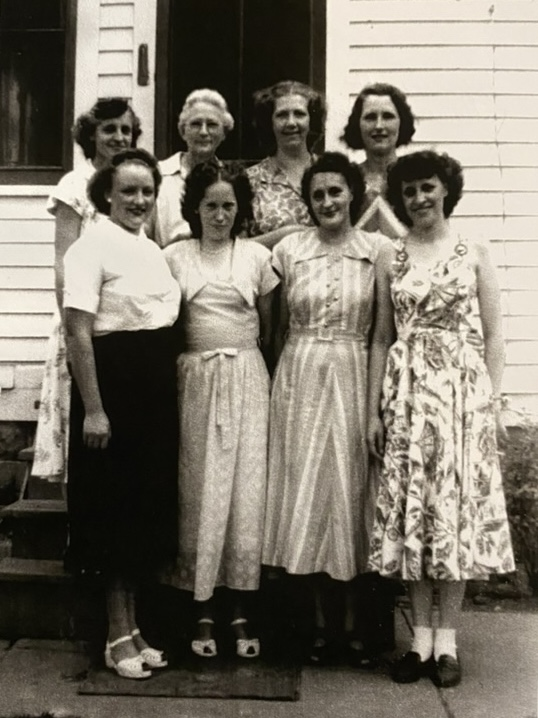
\includegraphics[width=0.85\linewidth,height=\textheight,keepaspectratio]{images/Akou24.jpeg}

}

\caption[Lila with members of the Schneider family, circa 1952.]{Lila
with members of the Schneider family, circa 1952. Top row from the left:
Helen, Minnie (Herman's aunt), Lila, Elvera (wife of Herman's brother,
Raymond); Bottom row: Charlotte (wife of Herman's brother, John),
Myrtle, Nora, and Grace}

\end{figure}%

Lila wasn't sure how to respond. Was it an innocent question or was
Myrtle judging her for having another baby? ``Her name is Hazel, after
my mother.''

``That's lovely,'' Myrtle replied. ``I guess I never knew what your
mother's name was.''

Lila tried to relax. When she was pregnant the first time, the
Schneiders had been her saving grace. As they ate dinner (sausages and
sauerkraut, which she had never enjoyed), they talked about Camp McCoy.
For a few years, it had been used for German prisoners of war, but now
the prisoners were gone and a new war had just started; the base was
filling up again with soldiers and their families. After the meal, when
Hazel was napping and Lila was helping with the dishes, Myrtle said,
``Herman wants you to come back. Johnny and Alice need you. I don't know
why you went to La Crosse when you have a home right here. You should be
here with Herman and your children.'' She meant well. But the thought of
going back to the farm---to chores and no hot water and no jokes and no
flirting---made Lila feel exhausted deep in her bones. Herman had not
tried to find her in La Crosse. Maybe he also recognized that they were
never a good match. It just wasn't enough.

Lila told Myrtle, ``I need to get back to the train station. The last
train is at 7:45.'' She didn't tell her that she was pregnant again.

Myrtle made her promise that she would return to West Salem in two
weeks. ``I'll ask Herman to let us have Johnny and Alice for the
weekend. They will be so happy to see you and Myrtle Joyce!''

\section{Notes}\label{notes-51}

In this chapter, Lila reaches a tipping point: pregnant again, she
realizes that she cannot manage another child without help and returns
to the Schneiders. My experience with the Schneiders as a child was
mostly with Myrtle and John Schneider and their extended family (grown
children and grandchildren). I found Myrtle to be very judgmental, but
as I poured through names and dates and family photographs (Nora worked
in a photography studio), I formed an impression that the Schneider
family as a whole was much more caring and down-to-earth.

During the process of writing the main manuscript, I reached out to
Linda Wood (daughter of Gladys Schneider, Herman's younger sister) to
see if she had any memories of Lila. She did not, but she gave me some
useful background information about her parents, other Schneider family
members, West Salem, and Camp McCoy. We've kept in touch. She confirmed
my impression that Gladys was an outgoing and kind person and a good
mother.

For more information, see Aine Collier\footnote{\citeproc{ref-collier2010a}{\emph{The
  Humble Little Condom: A History} (Amherst: Prometheus, 2010)}.},
Fournier\footnote{\citeproc{ref-fournier2008a}{\emph{Fort McCoy}}.}, and
Leslie J. Reagan\footnote{\citeproc{ref-reagan2022a}{\emph{When Abortion
  Was a Crime: Women, Medicine, and Law in the United States,
  1867--1973} (Berkeley: University of California Press, 2022)}.}.

\bookmarksetup{startatroot}

\chapter{Chapter Fifty}\label{chapter-fifty}

Lila was skeptical about Myrtle's plans, but she went back to visit as
promised. Johnny remembered her immediately and gave her a long hug.
Since she had missed his birthday, she gave him a slinky as a gift. The
children were fascinated and played with it for hours. Alice was shy;
she was more interested in the new baby than in her mother. Myrtle said,
``Give her a little time\ldots she'll warm up.'' By the end of the
visit, Alice was sitting in her lap. Until that moment, Lila had not
realized just how much she had missed her two other children. It was
like part of her soul had been ripped out when Helen sent them to live
with Herman.

For the next visit, Myrtle invited Gladys. She gave Lila a big hug and
said, ``I'm so glad to see you again.'' Lila was ashamed that they had
fallen out of touch; she could have written her letters. Gladys had a
little boy who was the same age as Hazel. After church, they traded
funny stories about being mothers. She was such a joy to be around. The
children also swirled around her like honeybees around their queen.

``Look at this carrot I dug up, Aunt Gladys\ldots it looks like a little
person!''

``Watch me do a somersault\ldots now watch me do a cartwheel!''

When the older children wanted to play baseball, they asked her to be
their pitcher. One visit turned into another until Lila was taking the
train to West Salem nearly every Sunday.

It took weeks for the Schneiders to realize that Lila was pregnant; they
just assumed that she was gaining weight. Myrtle was the one who finally
confronted her. When Lila responded, ``Yes, I am pregnant,'' Myrtle had
tears in her eyes. ``How could you do this? I just want you to be happy
and straighten things out with Herman and now you're having another baby
that is not even his.'' Lila froze. She had let her guard down, but
Myrtle was no better than Veda. She had been such a good friend when she
was pregnant with Myrtle Joyce. It was a punch in the gut to realize
that she had stopped being a friend as soon as Lila became part of the
Schneider family. Family was Myrtle's whole life; she assumed that Lila
felt the same way.

Before the confrontation with Myrtle, Gladys had asked Lila to spend
Christmas at her house and Lila had agreed. December was a lonely time
of the year in La Crosse. The bar would be closed, and Emma would be
busy with her own children and grandchildren. Although she tried not to
think about it, December also reminded Lila of the rape: Christmas
lights, people laughing, clusters of soldiers. Every dumpster felt like
a threat. The year before, she had white-knuckled her way through the
month. The only way she could sleep was by drinking shots before bed. It
made her stomach sour, but it kept the nightmares away.

When Lila took the train for Christmas it was packed with college
students going home for the holidays. It was easy to recognize them with
their sweater sets and carefree laughter. She wondered what it would be
like to have that kind of life. Watching the other passengers was her
favorite thing about riding the train. Since she and the children were
staying in West Salem for a few days and going to church, Lila had
packed their best outfits in a plaid suitcase that she had found in a
secondhand shop. It fit neatly under their seat.

Lila had not considered that Herman would be at church. He entered just
a few moments before the service started and sat down next to her
without saying a word. She felt like her heart was going to leap out of
her throat. Was he angry? Did he want to talk? What would they say? With
her mind racing, she barely heard the songs or the sermon. Herman was
warm beside her and smelled like soap and hay. He didn't sing along with
the hymns. Lila wanted so badly just to hear his voice, but when the
service ended, he left without saying anything. Lila felt crushed. She
wanted to be desired. She wanted to be missed.

She was relieved when Herman joined them for dinner. Nora and her family
were there too. The house was chaos from all of the children laughing
and running around; their glee was infectious. Gladys had made Christmas
crackers for the children to open after dinner. The best way to open
them was to have two people pull on the ends, which caused the rolls of
cardboard covered with shiny paper to open with a bang.

\begin{quote}
What do you call a cat that lives in the desert?\\
\emph{Sandy claws!}\\
\strut \\
Why does Santa have three gardens?\\
\emph{So he can ho, ho, ho!}\\
\strut \\
What do Santa's little helpers learn at school?\\
\emph{The elf-abet!}
\end{quote}

Lila groaned over the first few jokes, but the children were delighted.
By the end, everyone was in tears from laughing so hard. They drank hot
chocolate (with mint schnapps for the adults) and stayed up late. At the
end of the evening, Lila was standing in the kitchen with Gladys and
Nora. Herman was already wearing his coat when he gave Lila a kiss on
the cheek. He smiled and then walked out the door without saying a word.

\section{Notes}\label{notes-52}

``Christmas crackers'' are not as common in the United States as in the
United Kingdom (where they were invented), but some people make and open
them for Christmas. I included these jokes to remind the reader that
Lila has a sense of humor. She is weighed down by many challenges but
(like any person) still desires companionship and fun.

The culture of drinking is very strong in Wisconsin, especially around
La Crosse: a college town with a large military base nearby and a large
German-heritage population (e.g., the Schneiders). I was introduced to
alcohol when I was still in diapers.

For more information, see Olde English Crackers\footnote{\citeproc{ref-oldenglishcrackers2024a}{{``How
  to Make Christmas Crackers: A DIY Guide''} (Olde English Crackers,
  2024),
  \url{https://www.oldenglishcrackers.com/how-to-make-christmas-crackers/}}.},
Deirdre Clemente\footnote{\citeproc{ref-clemente2014a}{\emph{Dress
  Casual: How College Students Redefined American Style} (Chapel Hill:
  University of North Carolina Press, 2014)}.}, Jim Draeger and Mark
Speltz\footnote{\citeproc{ref-draeger2012a}{\emph{Bottoms up: A Toast to
  Wisconsin's Historic Bars and Breweries} (Madison: Wisconsin
  Historical Society Press, 2012)}.}, Gilbert Ford\footnote{\citeproc{ref-ford2016a}{\emph{The
  Marvelous Thing That Came from a Spring: The Accidental Invention of
  the Toy That Swept the Nation} (New York: Atheneum Books for Young
  Readers, 2016)}.}, and Dan Shafer\footnote{\citeproc{ref-shafer2016a}{{``Most
  of America's Drunkest Cities Are in Wisconsin,''} \emph{Milwaukee
  Magazine}, May 17, 2016,
  \url{https://www.milwaukeemag.com/most-of-americas-drunkest-cities-are-in-wisconsin/}}.}.

\bookmarksetup{startatroot}

\chapter{Chapter Fifty-One}\label{chapter-fifty-one}

What did Herman's kiss mean? The question rattled in Lila's mind. Did he
forgive her? Did he want her to come back? Maybe it just meant
``goodbye.'' Nora and Gladys had seen the kiss, but they offered no
explanations.

There was heavy snow in January. Between the snow, the pregnancy, and
carrying Hazel (who was walking but not old enough to walk by herself in
the street), it was getting difficult for Lila to travel more than a few
blocks. By the time the blizzards eased up and Lila was able to go back
to West Salem, it was already the end of February. Gladys was visibly
relieved to see her. She welcomed the children and brewed a pot of tea
to warm them up. By the time it was ready, the children were off
playing. After some easy conversation, Gladys put her hands over Lila's.
(Oh no, Lila thought\ldots here comes another ``talk.'') Gladys looked
her in the eye and said, ``Lila, I truly do care about you. I don't know
what happened between you and Herman, and it's not my place to judge. I
love him as my brother, and I love you as my sister.'' Lila felt tears
welling up. She didn't want to be a burden or to break down in front of
Gladys.

``What can I do to help you, Lila? Myrtle Joyce and Hazel can stay with
us while you're in the hospital. I don't know what else you might
need.'' It was like talking with Emma. Unlike Myrtle, Gladys didn't jump
to conclusions or make demands. She just listened.

Lila started to cry, and Gladys offered her a handkerchief. Eventually,
Lila replied, ``Maybe I should move back to West Salem.''

``Is that what you want?'' said Gladys. ``Would that make you happy?''

A flood of emotions was building in her heart---sadness, anger, grief,
anguish---maybe even hope. Gladys didn't press her for an answer. Lila
said, ``I just don't know. I don't think Herman and I belong together,
but how would I find a job if I moved back here?''

With her encouragement, Lila went to La Crosse Hospital to ask for an
appointment. It had never occurred to her to see a doctor before going
into labor. Gladys said that it was called ``prenatal care.'' When the
doctor opened her file, his eyebrows furrowed in concentration. ``I'm
glad you came in, Mrs.~Schneider. Hopefully, we can make this delivery
easier for you than the last time.'' He scheduled surgery for April
sixth but told her to return immediately if she noticed any signs of
labor. Lila promised that she would.

Lila worked at the bar right until the end. She was grateful to have the
income and to be around people, even though the men had stopped flirting
with her. A small group of regulars who had known one another since
childhood were singing drinking songs at the bar on Friday nights. Some
of them were funny and some were tearjerkers. One of her favorite songs
was ``My Bonnie Lies Over the Ocean.''

\begin{quote}
My bonnie lies over the ocean,\\
My bonnie lies over the sea,\\
My bonnie lies over the ocean,\\
Oh, bring back my bonnie to me!
\end{quote}

During the chorus, everyone sitting at the bar would sway back and forth
to the words. When her fifth child was born---another girl---Lila
decided to name her Bonnie. Naming them after friends and family had
never done any good. It was time for something new.

\section{Notes}\label{notes-53}

After a long series of challenges (and sometimes poor decisions), Lila
has grown wary of ``the talk'' from friends and family members. The
unconditional acceptance she feels from Gladys allows her to take some
bits of advice, like pursuing prenatal care.

I don't know if Lila ever received any kind of mental health support; it
is unlikely since the concept of ``Rape Trauma Syndrome'' was coined in
1974 and PTSD in the 1980s.

For more information, see Ed Cray\footnote{\citeproc{ref-cray1999a}{\emph{The
  Erotic Muse: American Bawdy Songs} (Champaign: University of Illinois
  Press, 1999)}.}, Judith Lewis Herman\footnote{\citeproc{ref-herman1992a}{\emph{Trauma
  and Recovery: The Aftermath of Violence---from Domestic Abuse to
  Political Terror} (New York: Basic Books, 1992)}.}, and Marika
Seigel\footnote{\citeproc{ref-seigel2013a}{\emph{Expecting: A Brief
  History of Pregnancy Advice} (University of Chicago Press, 2013)}.}.

\bookmarksetup{startatroot}

\chapter{Chapter Fifty-Two}\label{chapter-fifty-two}

Lila had given up her apartment after she found a house to rent on
French Island. The owner had been diagnosed with tuberculosis and needed
some time away to recover. Emma's sons had helped her move. Less than
three weeks after Bonnie arrived, Lila was back at work. It was the
first time she had been able to return to the same job after having a
baby. Lila was grateful, but she was also exhausted. Some of the
regulars cheered when she returned, but Betty (the curvy waitress)
pulled her into the storeroom and said, ``I'm worried about you,
Lila\ldots why are you back to work so soon?''

Lila shrugged. ``I need this job to support my children.''

Betty gave her a hug and vowed to help her as much as she could. After a
few weeks, Lila realized that Betty's ``help'' consisted mostly of
cashing out her tabs and taking the tips.

At the end of the month, Gladys visited with Myrtle Joyce and Hazel.
Lila felt ashamed that she had not been able to clean the house or bake
any treats. She was just too tired. Gladys said, ``Don't be silly. I'll
wash these dishes and you can enjoy a little time with your children.''
Myrtle Joyce was excited that the baby was a girl. ``I told you, Mom!''
After a few minutes, she said, ``I'm going to Emma's house to see if she
has any cookies.'' Before Lila could object, she was already out the
door. Her increasing independence made Lila nervous.

Gladys put two cups of tea on the table and said, ``Let me hold
Bonnie\ldots I'm sure Hazel would like to sit with you for a while.''
She was sucking her thumb when Lila pulled her into her lap. She laid
her head on Lila's chest and quickly fell asleep.

``I hope the girls haven't been too much trouble.''

``No trouble at all,'' said Gladys. ``If you don't mind, I think it
would be good for them to stay with us until the school year is finished
next month.''

``That's fine,'' said Lila. As much as she wanted them back home, she
knew that as soon as they returned it would be more work and more
expense. She wasn't sure that she could handle it.

Lila did her best to be attractive and outgoing at work. Her breasts
felt enormous in the uniform, even though she had purchased a new bra to
keep the ``girls'' under control. She began curling her hair and wearing
dark red lipstick. One of the regulars said she looked like Elizabeth
Taylor, but the cook---who everyone called Merlin---was not fooled. One
night after the dinner rush, he told Lila, ``You look like you've been
through a war\ldots I see the exhaustion in your eyes.'' Lila looked
down at the floor and said nothing. The next night, he slipped her a
package of pills in a tiny envelope. ``Try these for a week\ldots take
one at the start of your shift. If you like what it does, I can get you
more.'' After her experience with the thyroid medication, Lila was
skeptical that they would do anything.

She had no idea what was in the pills, but she decided to try one the
next night. To her surprise, she made it through her shift, picked
Bonnie up from Emma's house, and had enough energy to wash the dishes
before falling asleep. The next night was the same, and the night after
that. It was like a switch had flipped. She told Merlin that she wanted
more. ``Five dollars per week,'' he replied. It was a lot of money, but
she was tired of being so tired. They shook hands and settled the deal.

At the end of May, Lila took the train to West Salem. Gladys asked to
hold Bonnie and told her, ``You must be a good little sleeper\ldots your
mother looks fantastic!'' To Lila's surprise, Alice was there with
Myrtle Joyce and Hazel. All of her girls were together. She sat on the
floor, and they piled around her. For a moment, Lila was filled with
joy. When the children left to play again, Lila and Gladys sat down at
the kitchen table to have coffee and strawberry pie.

Gladys said casually, ``Herman asked me to take Alice. She was having a
tough time on the farm.''

``Oh?'' said Lila. ``What kind of trouble?''

``Herman didn't say, just that it would be better if Alice stayed with
you.''

Lila had mixed feelings. She was thrilled at the idea of having Alice
back, but could she really take care of four children? Myrtle Joyce was
the only one old enough to be in school. Regardless of her feelings, she
felt like she didn't have a choice. If the Schneider family trusted her
enough to have Alice back, she better not disappoint them.

\section{Notes}\label{notes-54}

Much of this chapter is based on my own experience as a worker and
single mother. I've never used recreational drugs, but I remember when I
started drinking coffee daily (after my last child was born). I wondered
how I had managed without it.

During World War II, the Nazis gave soldiers meth to keep them alert and
motivated beyond normal levels of human endurance. In response, the US
military began experimenting with amphetamines; some soldiers developed
addictions and sought out the drug when they returned home. In the
1930s, 1940s, and 1950s, doctors prescribed amphetamines (mostly to
women) as an appetite suppressant and treatment for depression. As a
street drug, it became known as ``speed'' for its ability to keep
exhausted workers on their feet.

I'm not certain that Lila used speed; however, she did lose a lot of
weight a few years before her death (from causes that are consistent
with amphetamine abuse).

For more information, see Peter Andreas\footnote{\citeproc{ref-andreas2020a}{\emph{Killers
  High: A History of War in Six Drugs} (Oxford University Press, 2020)}.},
Lester Grinspoon and Peter Hedblom\footnote{\citeproc{ref-grinspoon1975a}{\emph{The
  Speed Culture: Amphetamine Use and Abuse in America} (Cambridge:
  Harvard University Press, 1975)}.}, and Nicolas Rasmussen\footnote{\citeproc{ref-rasmussen2008a}{{``America's
  First Amphetamine Epidemic, 1929--1971,''} \emph{American Journal of
  Public Health} 98, no. 6 (2008): 974--85}.}.

\bookmarksetup{startatroot}

\chapter{Chapter Fifty-Three}\label{chapter-fifty-three}

On the first weekend in June, Gladys drove to French Island with Myrtle
Joyce, Hazel, and Alice. The sun was brilliant that day; Lila hoped that
it was a sign of good things to come. Gladys hugged them all and told
Myrtle to ``be a good helper.'' Emma was delighted to see the children
again and made them a cake covered with shredded coconut for decoration.
It looked like an enormous dandelion ready for the wind to carry the
seeds away.

That summer, Herman began driving Johnny to Emma's house so he could see
his sisters. Gladys had given him Emma's address. Lila had hoped that
they would get a chance to talk, but he always visited the island while
she was working. Was he avoiding her? As usual, Lila found it nearly
impossible to know what he was thinking.

As her strength returned from having Bonnie, she found that the pills
from Merlin were a little too strong. She had tried to quit taking them,
but the sudden lack of energy scared her; she could barely get out of
bed. With the pills, she could work and take care of the children, but
she was plagued by insomnia, worse than anything she had experienced
before. She knew that she needed to sleep. She just could not do it.
When she told Merlin about it, he said, ``Yes, that can happen
sometimes. You might need a drink to unwind before bed.'' She purchased
a bottle of whiskey and stashed it in the highest cupboard in the
kitchen. She hated the thought that she might turn herself into a drunk
like her mother but had no idea what else to try.

Merlin's solution was effective but tricky. She needed to drink enough
to fall asleep, but not so much that it would keep her from waking up
when the girls needed her. She couldn't take the first drink at
work---she discovered that it gave her an intense desire for sex---but
she didn't want to drink in front of the children. She decided that she
would wait until they were asleep. It took her weeks to find a routine
that usually worked.

In the spring, Lila had to find a new place to live; the owner of the
little house on French Island had recovered and was eager to move back
in. It took Lila nearly a month to find a new apartment. Nobody wanted
to rent to a single mother working in a bar, especially when they
learned how many children she had. The apartment was in an old house
that was falling apart, but the children loved it. It had two stories
and long staircases on both sides. For hours they would race one another
up the stairs and down the other side. One day Myrtle found a litter of
stray kittens and begged to keep them. For a moment, Lila flashed back
to being a child. She was not much younger than Myrtle when she begged
her mother to let her keep Annabelle; now she was the mother. Lost in
her thoughts, she told Myrtle that they could keep just one.

\begin{figure}[H]

{\centering 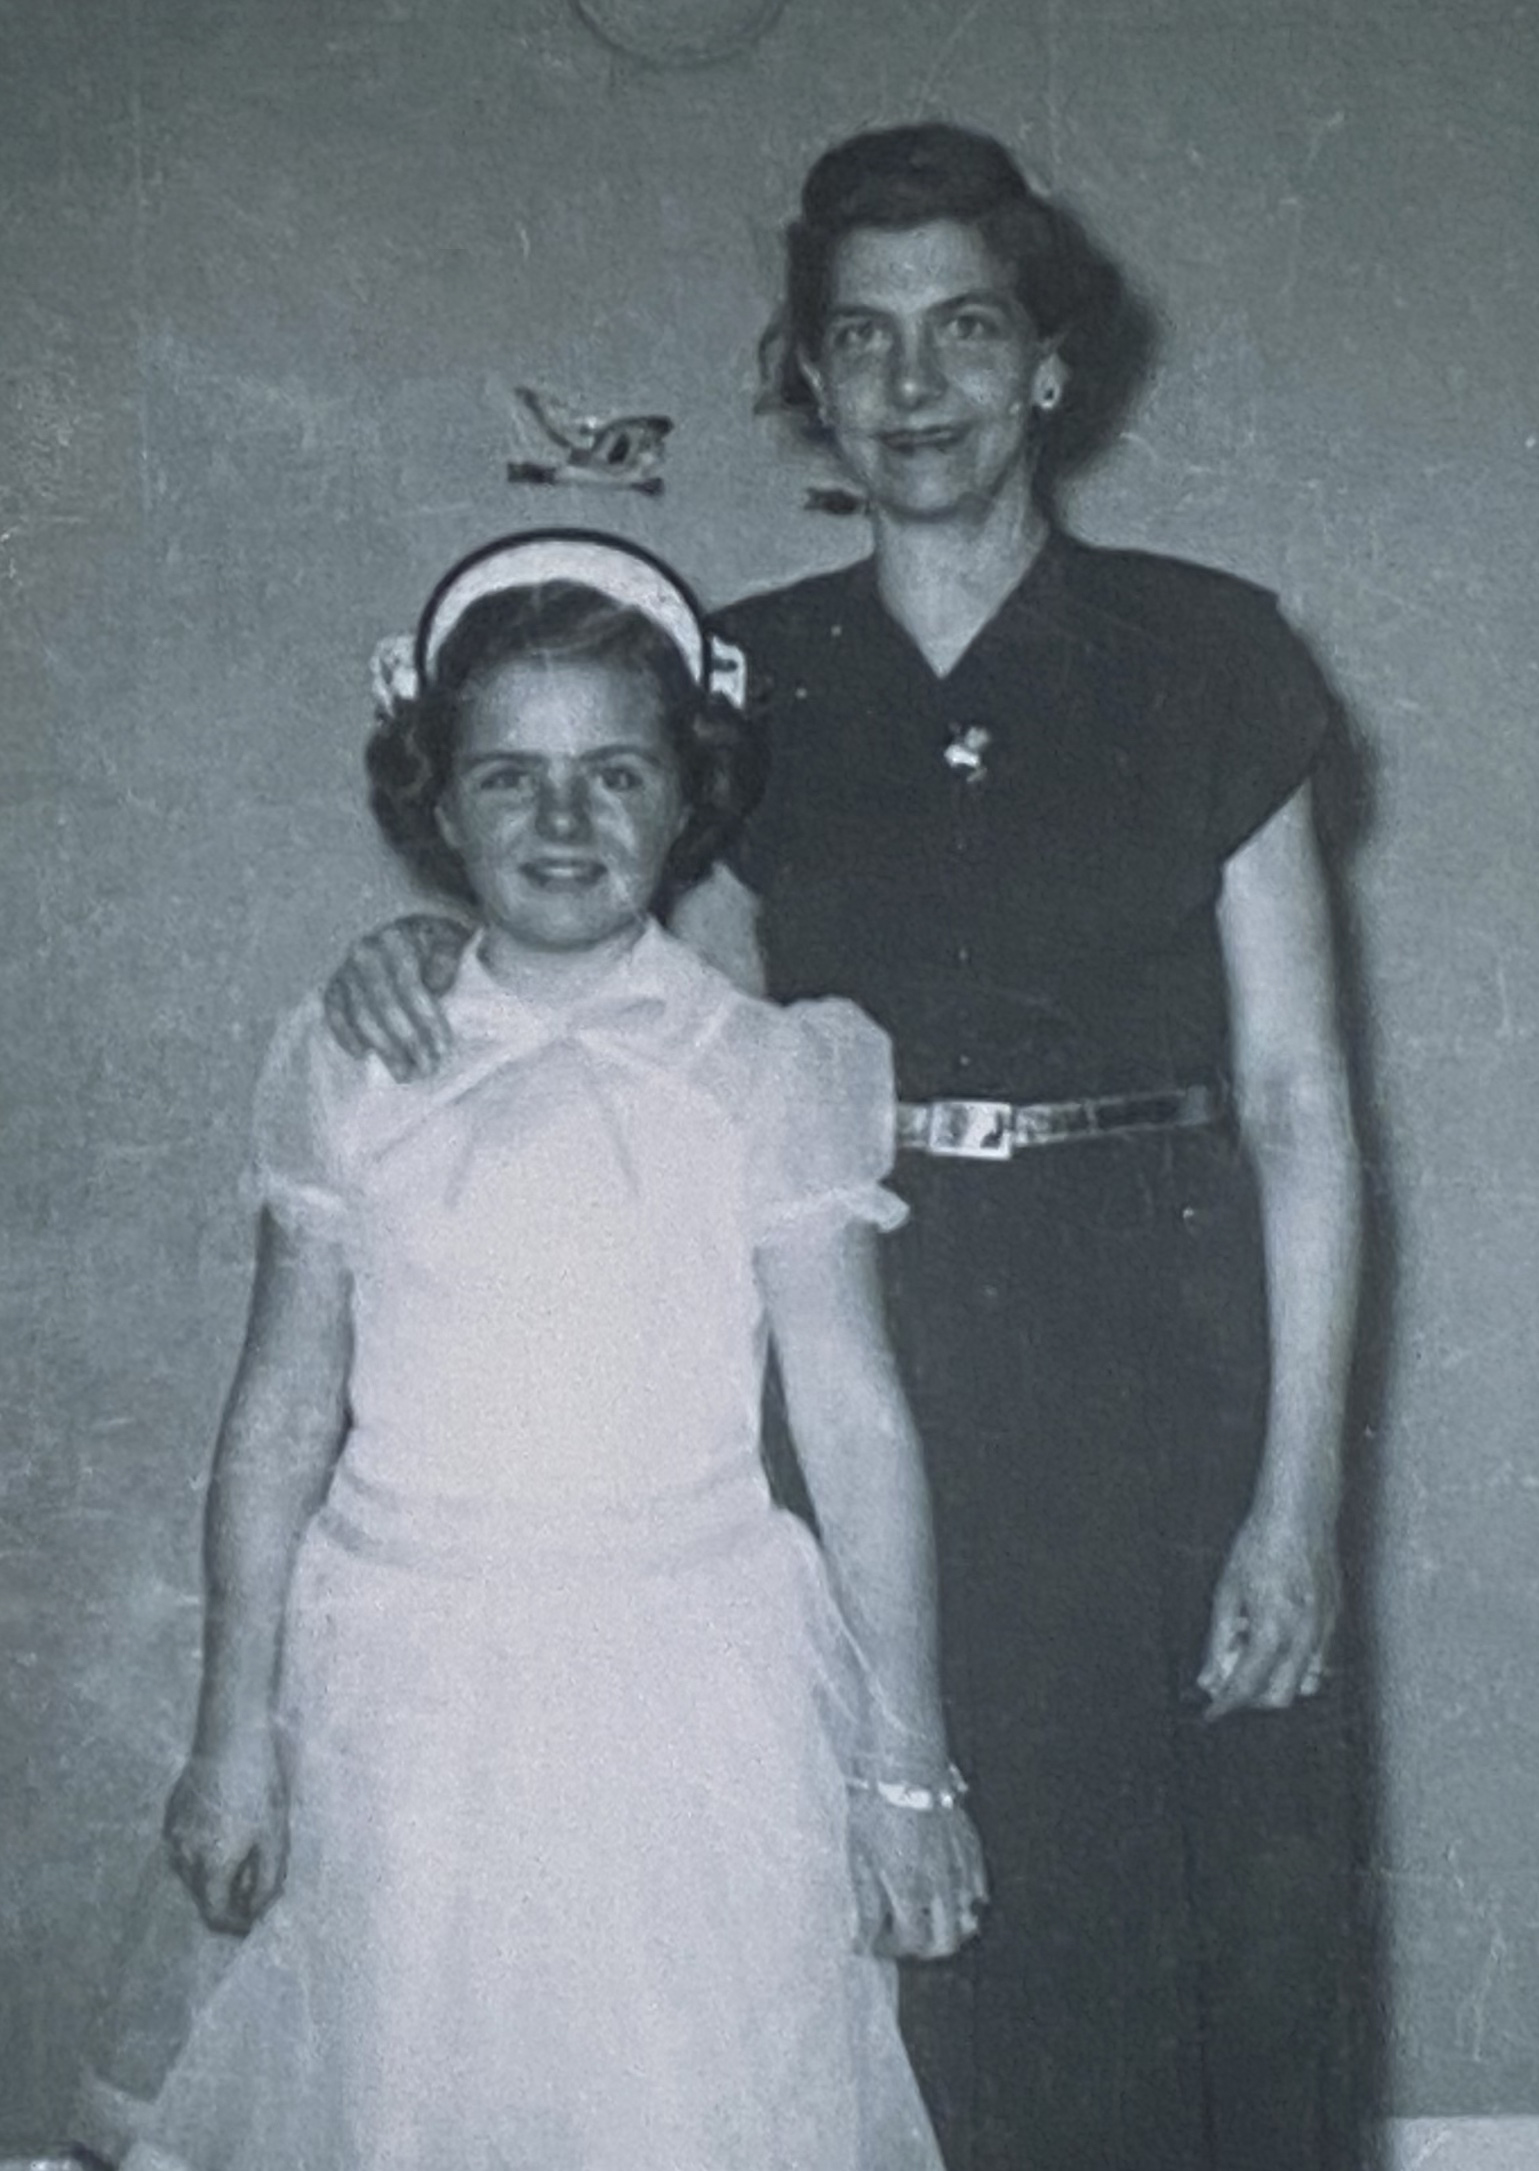
\includegraphics[width=0.55\linewidth,height=\textheight,keepaspectratio]{images/Akou25rt.jpg}

}

\caption{Lila and her niece, Patty Metcalf, circa 1953}

\end{figure}%

Much of that year and the next were a blur. She reconnected with
Veda---not because she trusted her but to prove that Veda was wrong
about her as a mother. Myrtle Joyce was thrilled to see her cousins
again. Aunt Hattie died that year; Veda was horrified when Lila refused
to go to the funeral. She couldn't afford to miss work, but she enjoyed
the look on Veda's face when she told her she wasn't going. She didn't
understand why Veda still admired her.

In truth, Lila's life was just as much of a struggle as ever. There were
months when she could barely afford the rent. At work, she snuck
half-eaten meals out of the garbage so she could leave the food at home
for the children. Emma gave the children baths and made sure they had
clothes to wear. Later, she reflected on how much Emma had loved all of
them; she regretted that she was never able to return her many favors.
When Alice turned five, Myrtle Joyce was the one who made their lunches
and walked Alice to school.

Some of the regulars at the bar could not keep their hands to
themselves. Although Lila had recoiled the first time Hank (the owner)
touched her when she was behind the bar, she had grown used to the
constant brushing and groping. One night, one of the regulars motioned
for her to lean over. She assumed he wanted to order another drink, but
he whispered into her ear, ``Ten dollars.'' Ten dollars for what? She
was too busy at the time to think about it, so he was already gone by
the time she understood. The next time he offered ``ten dollars'' she
agreed to meet him behind the building after her shift. Unlike Jack, he
didn't wear a rubber.

That time when she got pregnant, it ended with a long and painful night
in the bathroom. She didn't go to the doctor. In fact, she didn't say
anything to anyone about it. The miscarriage was both a relief and a
dark shame. The voice in her head was brutal. Slut! Whore! Why did you
allow this to happen?! Couldn't you just keep your legs together? For
weeks she worked in a fog of regret and self-loathing. The sex was not
rape, but there was no love in the transaction. She had just needed the
money to pay the rent.

\section{Notes}\label{notes-55}

The beginning of this chapter is based mostly on stories from my mother
and aunts, especially the house with the long staircases on both sides.
I begged her for a kitten when I was little. My children begged me for
one. It feels like an experience that circles through the generations of
my mother's family.

This chapter reminds us just how fractured Lila's relationships have
become. Veda is the only member of the Slaback family that Lila is still
communicating with (barely). She has been separated from her husband for
several years with little hope of reconciliation. Her life as a waitress
in a bar is so filled with sexual harassment that it barely registers. I
don't know if Lila was ever paid for sex, but it would have been easy
for her to slip into casual prostitution.

For more information, see Kylie Agllias\footnote{\citeproc{ref-agllias2016a}{\emph{Family
  Estrangement: A Matter of Perspective} (Oxford: Taylor \& Francis,
  2016)}.}, Barry M. Dank and Roberto Refinetti, eds.\footnote{\citeproc{ref-dank2018a}{\emph{Sex
  Work and Sex Workers} (Oxford: Taylor \& Francis, 2018)}.}, and Fern
Schumer Chapman\footnote{\citeproc{ref-chapman2021a}{\emph{Brothers,
  Sisters, Strangers: Sibling Estrangement and the Road to
  Reconciliation} (New York: Penguin Publishing, 2021)}.}.

\bookmarksetup{startatroot}

\chapter{Chapter Fifty-Four}\label{chapter-fifty-four}

The next person she had sex with was Merlin. The pills were losing
effectiveness; once again, she was tired all the time. He said he could
fix that, but it would cost extra. How much? Two dollars per week. She
must have looked shocked or desperate because after a few moments he
added, ``If you can't afford it, we can set up a trade.''

Merlin had been a soldier. He had lost one of his ears to a sniper's
bullet, but he wore a fake and kept his hair a bit long. Most people
didn't notice. Lila wasn't sure why he had decided to work in a bar. He
didn't sing or tell jokes. He didn't even drink. He made the hamburgers
and cheese curds and Reuben sandwiches without complaint, but it didn't
take much skill to be that kind of cook. Before he started working,
there had been a series of cooks who quit after a few weeks. The job was
boredom punctuated by burns from the deep fryer. Later, Merlin told her
that he just enjoyed watching people: the regulars, the waitresses, the
brawlers, and the criers. He thought they were all fascinating. He
admitted that he made more money selling pills than he did as a cook.
Everyone at the bar was a potential customer.

The trade with Merlin was a monthly night of sex, but it was never
impulsive. He didn't want to wear rubbers but told her that if they had
sex right after her period ended, she wouldn't get pregnant. Could it
really work? She had never heard of it before. After a few months, she
started to enjoy their time together. Like Jack, Merlin never gave any
indication that he wanted to get married or be a father, yet Lila found
herself fantasizing about sharing a life with him---cooking for him,
waking up next to him, having someone who could share the burdens and
joys of being a parent. Merlin was not fazed by her life as a single
mother. He knew that she worked in a bar and didn't judge her for it;
she thought it was the best she could hope for.

There was just one problem with Merlin's plan: Lila's cycle was no
longer regular. Was it the pills? Was it normal for her age? She had no
idea. One time her period returned after just three weeks. Another time
it took seven weeks. She wept from relief when she started bleeding
again. What was she supposed to do about the bargain? One month she
didn't have her period and decided just to tell Merlin that it was
``time.''

Late in the summer of 1953, Lila realized that she was pregnant. She
didn't want to say anything to Merlin, but she saw him every time she
had to pick up a tray from the kitchen. The secret was eating away at
her. It didn't take him long to ask what was wrong. When she told Merlin
that she was pregnant, he froze. After a pause that felt like hours, he
said, ``How is that possible?'' Lila started to cry. She couldn't cry at
work, so she walked out to the back of the building. A few minutes
later, Merlin followed her. ``You can't take those pills while you're
pregnant\ldots you need to start tapering down right away.''

By the time she went to the doctor, she was no longer taking them. It
had been a hard adjustment. The fatigue came roaring back, and she felt
a crushing sense of sadness and doom. She was gaining weight (Merlin
told her it was good for the baby), and the apartment was an absolute
mess. She had put Myrtle Joyce in charge of washing the dishes, but they
often sat in the sink for days. A few times she was so angry that she
hit her with the cord from the iron. She felt bad for lashing out; it
was terrifying to be so out of control. Alice was wetting the bed and
Bonnie was teething. Lila had been through difficult times, but this was
a new level of difficult.

At her appointment, the doctor said, ``Your blood pressure is higher
than I would like. I need to see you again in one week.'' What did that
mean? The doctor didn't explain.

The next time he said, ``Mrs.~Schneider\ldots I'm concerned that you're
developing toxemia. Have you ever heard of that?''

Lila shook her head to say no.

``Since the start of this pregnancy, have you had any dizziness or
vomiting?''

``A little,'' she said, thinking that it was probably because she had
stopped taking the pills. In that moment, she wanted them so badly.

The doctor asked her to raise her legs and pressed his fingers into her
ankles. ``Have you had any headaches or blurry vision?'' Merlin had
warned her that she would ``feel like crap'' for a while, but he hadn't
been very specific. She had been so focused on getting off the pills
that she hadn't really considered how the pregnancy itself was affecting
her.

After the doctor asked a few more questions he said,
``Mrs.~Schneider\ldots for the health of you and your baby, I want you
to go on bed rest. I want you to lay down and not get up for more than
one hour per day.''

Lila was shocked. What he was asking was impossible. ``But how will I
work? Who will take care of my children?''

Sternly, the doctor said, ``You need to figure this out right away. You
could have a stroke; you could be damaging your liver and
kidneys\ldots you could even die from this.'' He underscored his
seriousness by gripping her shoulders and staring straight into her
eyes.

When she left the hospital, her head was swimming. She went to work in a
daze and somehow managed to work her shift, but it would be her last
one. The next day she took the children to West Salem. When Myrtle Joyce
asked, ``Why are we not going to school today?'' Lila snapped back:
``Don't ask questions\ldots just do what you're told.'' When Gladys
answered the door, she knew immediately that something was wrong. She
told the children to go play and ushered Lila to the sofa. As Lila told
her what the doctor had said, Gladys's eyes grew wide with alarm. ``I'm
so sorry that this is happening to you, Lila. I'm glad you came to me
for help.''

By the next day, Gladys and Lila had come up with a plan. Myrtle Joyce
would go back to the orphanage in La Crosse. Alice would go with her
father. Hazel and Bonnie would go with a family that Gladys knew from
church. She reassured Lila that they were kind people who had a lot of
experience with children; they lived on a farm a few miles from town.
Gladys said that she would drop them off, but Lila said, ``No, it's my
responsibility. I want to be with them until the last possible moment.''
Gladys gave her the directions and the key to Carl's truck. They hugged
just before she drove off, and Lila said, ``Don't cry, Gladys. If you
cry\ldots I'm going to cry, and I don't think I'll be able to stop.''
Her throat was already clenching.

Lila didn't know if she would ever see her daughters again, but when she
left Hazel and Bonnie with the Jostads, she told them, ``I'll be back
soon.'' Dropping them off took all of Lila's remaining energy. Gladys
took Alice back to Herman. By then, Lila was getting so drowsy that
Gladys had to leave Myrtle Joyce and her own children with Nora so she
could drive her to La Crosse Hospital. They drove so fast that Gladys
was sure she would get a speeding ticket.

\section{Notes}\label{notes-56}

I've met people like Merlin before---men and women who appear to be
doing a certain job but are actually there for their own private
reasons. I used this chapter to speculate on how people like Merlin and
Lila end up in their positions as drug sellers and drug users. At any
time in her life, Lila could have walked away. I respect how hard she
fought to stay in her children's lives, even though it led her down some
very dark paths.

When my second pregnancy ended in a loss, I read the book \emph{Taking
Charge of Your Fertility} to help conceive my son. It builds on older
knowledge of the ``rhythm method'' of birth control, which works for
many people. Unfortunately, one problem with thyroid disorders is that
they tend to throw off the timing of the reproductive cycle. In the
1970s, toxemia was relabeled as ``hypertensive disorder of pregnancy.''
Today, it is called pre-eclampsia.

When I reconnected with one of my mother's sisters (June) in early 2020,
she told me about her memory of Lila dropping her off at the Jostad
house. They were kind people, but June and her younger sister
Bonnie---who always stayed together---did not see Lila again for two
years.

For more information, see Nancy Campbell\footnote{\citeproc{ref-campbell2000a}{\emph{Using
  Women: Gender, Drug Policy, and Social Justice} (New York: Routledge,
  2000)}.}, John Henry Tilden\footnote{\citeproc{ref-tilden1974a}{\emph{Toxemia,
  the Basic Cause of Disease: An Antidote to Fear, Frenzy, and the
  Popular Mania of Chasing After so-Called Cures} (Youngstown: Natural
  Hygiene Press, 1974)}.}, Thomas S. Weinberg, Gerhard Falk, and Ursula
Adler Falk\footnote{\citeproc{ref-weinberg2017a}{\emph{The American Drug
  Culture} (Thousand Oaks, California: SAGE Publications, 2017)}.}, and
Toni Weschler\footnote{\citeproc{ref-weschler1995a}{\emph{Taking Charge
  of Your Fertility: The Definitive Guide to Natural Birth Control,
  Pregnancy Achievement, and Reproductive Health} (New York:
  HarperCollins, 1995)}.}.

\bookmarksetup{startatroot}

\chapter{Chapter Fifty-Five}\label{chapter-fifty-five}

Lila was in the hospital for three months. When she entered, it was
winter; when she left, it was spring. Her son was born on March 8th,
1954. She had no idea what to name him. One of the attendants (who
struck Lila as being incredibly young in her little pink apron) said,
``I'll help you come up with a name!'' They chose Randy, which was a
popular new name for boys. Lila was relieved that he seemed to be
unharmed by the pills and the toxemia. He had a vigorous cry and was
hungry all the time. Concerned that he wasn't getting enough to eat, the
nurses made him extra bottles with evaporated milk and corn syrup.

One day, Myrtle and Carl arrived during visiting hours. Lila was
surprised to see them; in the last three years, they had rarely spoken.
Myrtle was wearing a striped dress that made her hips look enormous. She
was holding her handbag in front of her like a shield. She sat down in
the chair next to the bed, and Carl went into the hallway to find
another one. For a few moments, Lila stared at her while she looked at
the door, waiting for Carl to return. Finally, Myrtle cleared her throat
and said, ``I want you to give your son to us.''

``But why?'' said Lila. ``I won't be in the hospital for much longer.''

Myrtle glanced over at Carl, whose face was expressionless. Myrtle said,
``You can't keep living this way, Lila. Carl and I can adopt Randy and
raise him as one of our own. It's not right for your children to grow up
with a single mother.''

Lila wanted to scream; the only thing that stopped her was knowing that
the nurses would scold her for disturbing the ward and inject her with a
sedative. She stared at Myrtle with such intensity that Myrtle shifted
her gaze to the floor. After a few moments of silence, she stood up, and
Carl followed her to the door. Myrtle turned and said, ``I know you're
upset, but think about it, Lila. Randy will have a stable home and two
parents who love him.'' And with that, they left the room. Lila was so
enraged that the nurses gave her a sedative anyway.

Within a few days, her anger turned to sorrow. Myrtle was right. She
wasn't doing her children any favors by clinging to them. She had tried
so hard to be a good mother, but it just wasn't enough. The grief of
that realization extended her stay in the hospital; the nurses were
worried about her fragile state of mind. By the time she was ready to be
discharged, she had decided that Myrtle and Carl could have her son. A
nurse brought her the adoption papers.

As she held Randy for the last time as his legal mother, the nurse said
that they would release him to the Schneiders. With a compassionate
tone, she said, ``I know this is hard, but you're doing the right thing.
The hospital will take care of the rest.''

Leaving the hospital without a child in her arms was the worst feeling
she could have imagined. She had never felt so ashamed and full of
grief. Gladys had visited her several times during her stay in the
hospital, but she was not there the morning Lila was discharged. A
social worker had given her money for a cab. She asked the driver to
stop at the apartment, but she was not surprised to find that her key no
longer worked. There had not been enough time (or money) to make
arrangements with the landlord. Now she had no home, no possessions, no
job, and all of her children were gone. Was she even still a mother? In
a fog of disbelief, she gave the driver directions to Emma's house.

Summer arrived early that year, but Lila felt so cold and completely
empty. How was she going to get Myrtle Joyce out of the orphanage again
when she could barely get out of the house? Emma urged her to go back to
the doctor. He was dismissive when she described how tired she was, but
when he felt her neck during the exam he said, ``Hmm\ldots you do have a
goiter. I'll write you a prescription.''

Lila froze and said, ``No pills; I don't want to take anything.''

The doctor forced her to take the prescription, but she never went to
the pharmacy.

Unable to bear the thought of walking across the bridge, Lila decided to
take the first job on French Island that she was offered. It was at the
tavern on Bainbridge Street, the one she had rejected after Hazel was
born. Nothing had changed; it was just as creepy as she remembered.
``Beggars can't be choosers,'' she thought ruefully. Without an income,
she had no hope of renting an apartment. Even Emma wouldn't tolerate her
forever.

\section{Notes}\label{notes-57}

In 1954, ``Randy'' was the thirty-third most popular name for newborn
boys in the United States. It was not a family name for the Slabacks or
the Schneiders.

In the 1950s, there was tremendous social pressure for women to marry
young and give birth only in the context of an intact, heterosexual,
nuclear family. Less than five percent of white women pursued single
motherhood. I knew Myrtle Schneider, who died when I was twenty years
old. She cared tremendously about her children but also had very rigid
values regarding birth and marriage. I respect her for taking care of
Randy when the Slabacks were unwilling to step up; however, she probably
put a lot of (well-meaning) pressure on Lila.

For more information, see BabyCenter\footnote{\citeproc{ref-babycenter2024a}{{``Most
  Popular Baby Names of 1954''} (BabyCenter, 2024),
  \url{https://www.babycenter.com/baby-names/most-popular/top-baby-names-1954}}.},
Ruth Feldstein\footnote{\citeproc{ref-feldstein2018a}{\emph{Motherhood
  in Black and White: Race and Sex in American Liberalism, 1930--1965}
  (Ithaca: Cornell University Press, 2018)}.}, Gabrielle
Glaser\footnote{\citeproc{ref-glaser2021a}{\emph{American Baby: A
  Mother, a Child, and the Secret History of Adoption} (New York:
  Penguin Publishing, 2021)}.}, and Jessica Weiss\footnote{\citeproc{ref-weiss2000a}{\emph{To
  Have and to Hold: Marriage, the Baby Boom, and Social Change}
  (University of Chicago Press, 2000)}.}.

\bookmarksetup{startatroot}

\chapter{Chapter Fifty-Six}\label{chapter-fifty-six}

The tavern was small with just one other waitress. Mildred never told
her how old she was, but Lila thought she must be at least in her
forties. She looked (as Merlin would have said) ``ridden hard and put
away wet'' with streaks of gray hair, sagging breasts, and a tight,
leathery face. Most of the men at the bar were older too: working men
who had retired from their jobs and moved to French Island for the
excellent fishing. The bar didn't have a full menu, so the owner's
brother doubled as the bartender and cook. It was smaller than the other
places Lila had worked and easily the most depressing. The light
fixtures were yellow from years of cigarette smoke; it was always dim
inside regardless of the weather.

Lila had enough energy to work (barely), but inside she felt like
something had broken. Maybe forever. One of the regulars had a son who
was a police officer in Prairie du Chien. He often drove up to La Crosse
to go fishing and drinking with his father. They both swore like sailors
and told horrible, vulgar jokes. He flirted with Lila but so did most of
the other men. Why did she agree to have sex with him? If she was being
honest, it wasn't really about the money (although he offered her more
than usual---twenty dollars). She did it just to feel alive; to see if
she could still feel something: desire, anger, happiness, grief.
Anything.

Emma had always been so kind and supportive, but her face fell when Lila
told her that she was pregnant again. At her first doctor's appointment,
her blood pressure was already high. The doctor told her that she would
have to stay in the hospital until the pregnancy ended or the baby was
born. By the time an orderly arrived with a wheelchair, her mind was as
lifeless as a rabbit in the mouth of a fox.

Lila was not the one who named her last child. Larry was taken away
immediately by the state of Wisconsin and placed into foster care. Her
health had been declining since the pregnancy with Randy, but this time
the doctors told her that she must not have another child; the stress on
her kidneys would kill her. The adoption triggered an investigation. A
social worker pressed her for information: where were her other
children?

She was shocked when the state charged her with child neglect for
leaving Hazel and Bonnie with the Jostads. The social worker pointed out
that they were not family and were not registered in the foster-care
system.

Lila said, ``How was I supposed to know? There wasn't time to
investigate before I dropped them off\ldots it was an emergency.''

The social worker had given her a handkerchief and it was already
soaked. She continued, ``I see your point of view, Lila, but we need to
sort this out. The state needs to ensure that your children are safe.''

When the state pressed Herman for information, he filed for divorce. He
had promised to treat Myrtle Joyce like his own child, but in court, he
only took responsibility for John and Alice. It was a bitter ending to
their marriage. Years before, Lila had given up getting back together,
but she was stunned to be divorced. Marriage was supposed to be forever.

She was also stunned when the state began giving her welfare; she had
never thought to ask for support. Faced with a choice between giving her
daughters up for adoption (minus Alice, who had been claimed by Herman)
or trying once more to raise them, she decided to give it her best. A
social worker helped her find a new apartment near Copeland Park, but
being a mother again was rough. Hazel was six years old, and Bonnie was
five. They had been away for two years and barely remembered her. Myrtle
Joyce was twelve years old and had a hot temper. It reminded Lila of her
own mother; sometimes, when Myrtle Joyce yelled, Lila felt like a small
child again. She had no idea how to repair the years of damage they had
all endured.

Lila eventually found another job in a bar. For the rest of her life,
she resisted taking any pills; however, she often drank to numb her
feelings, which felt like impossible burdens.

\begin{figure}[H]

{\centering 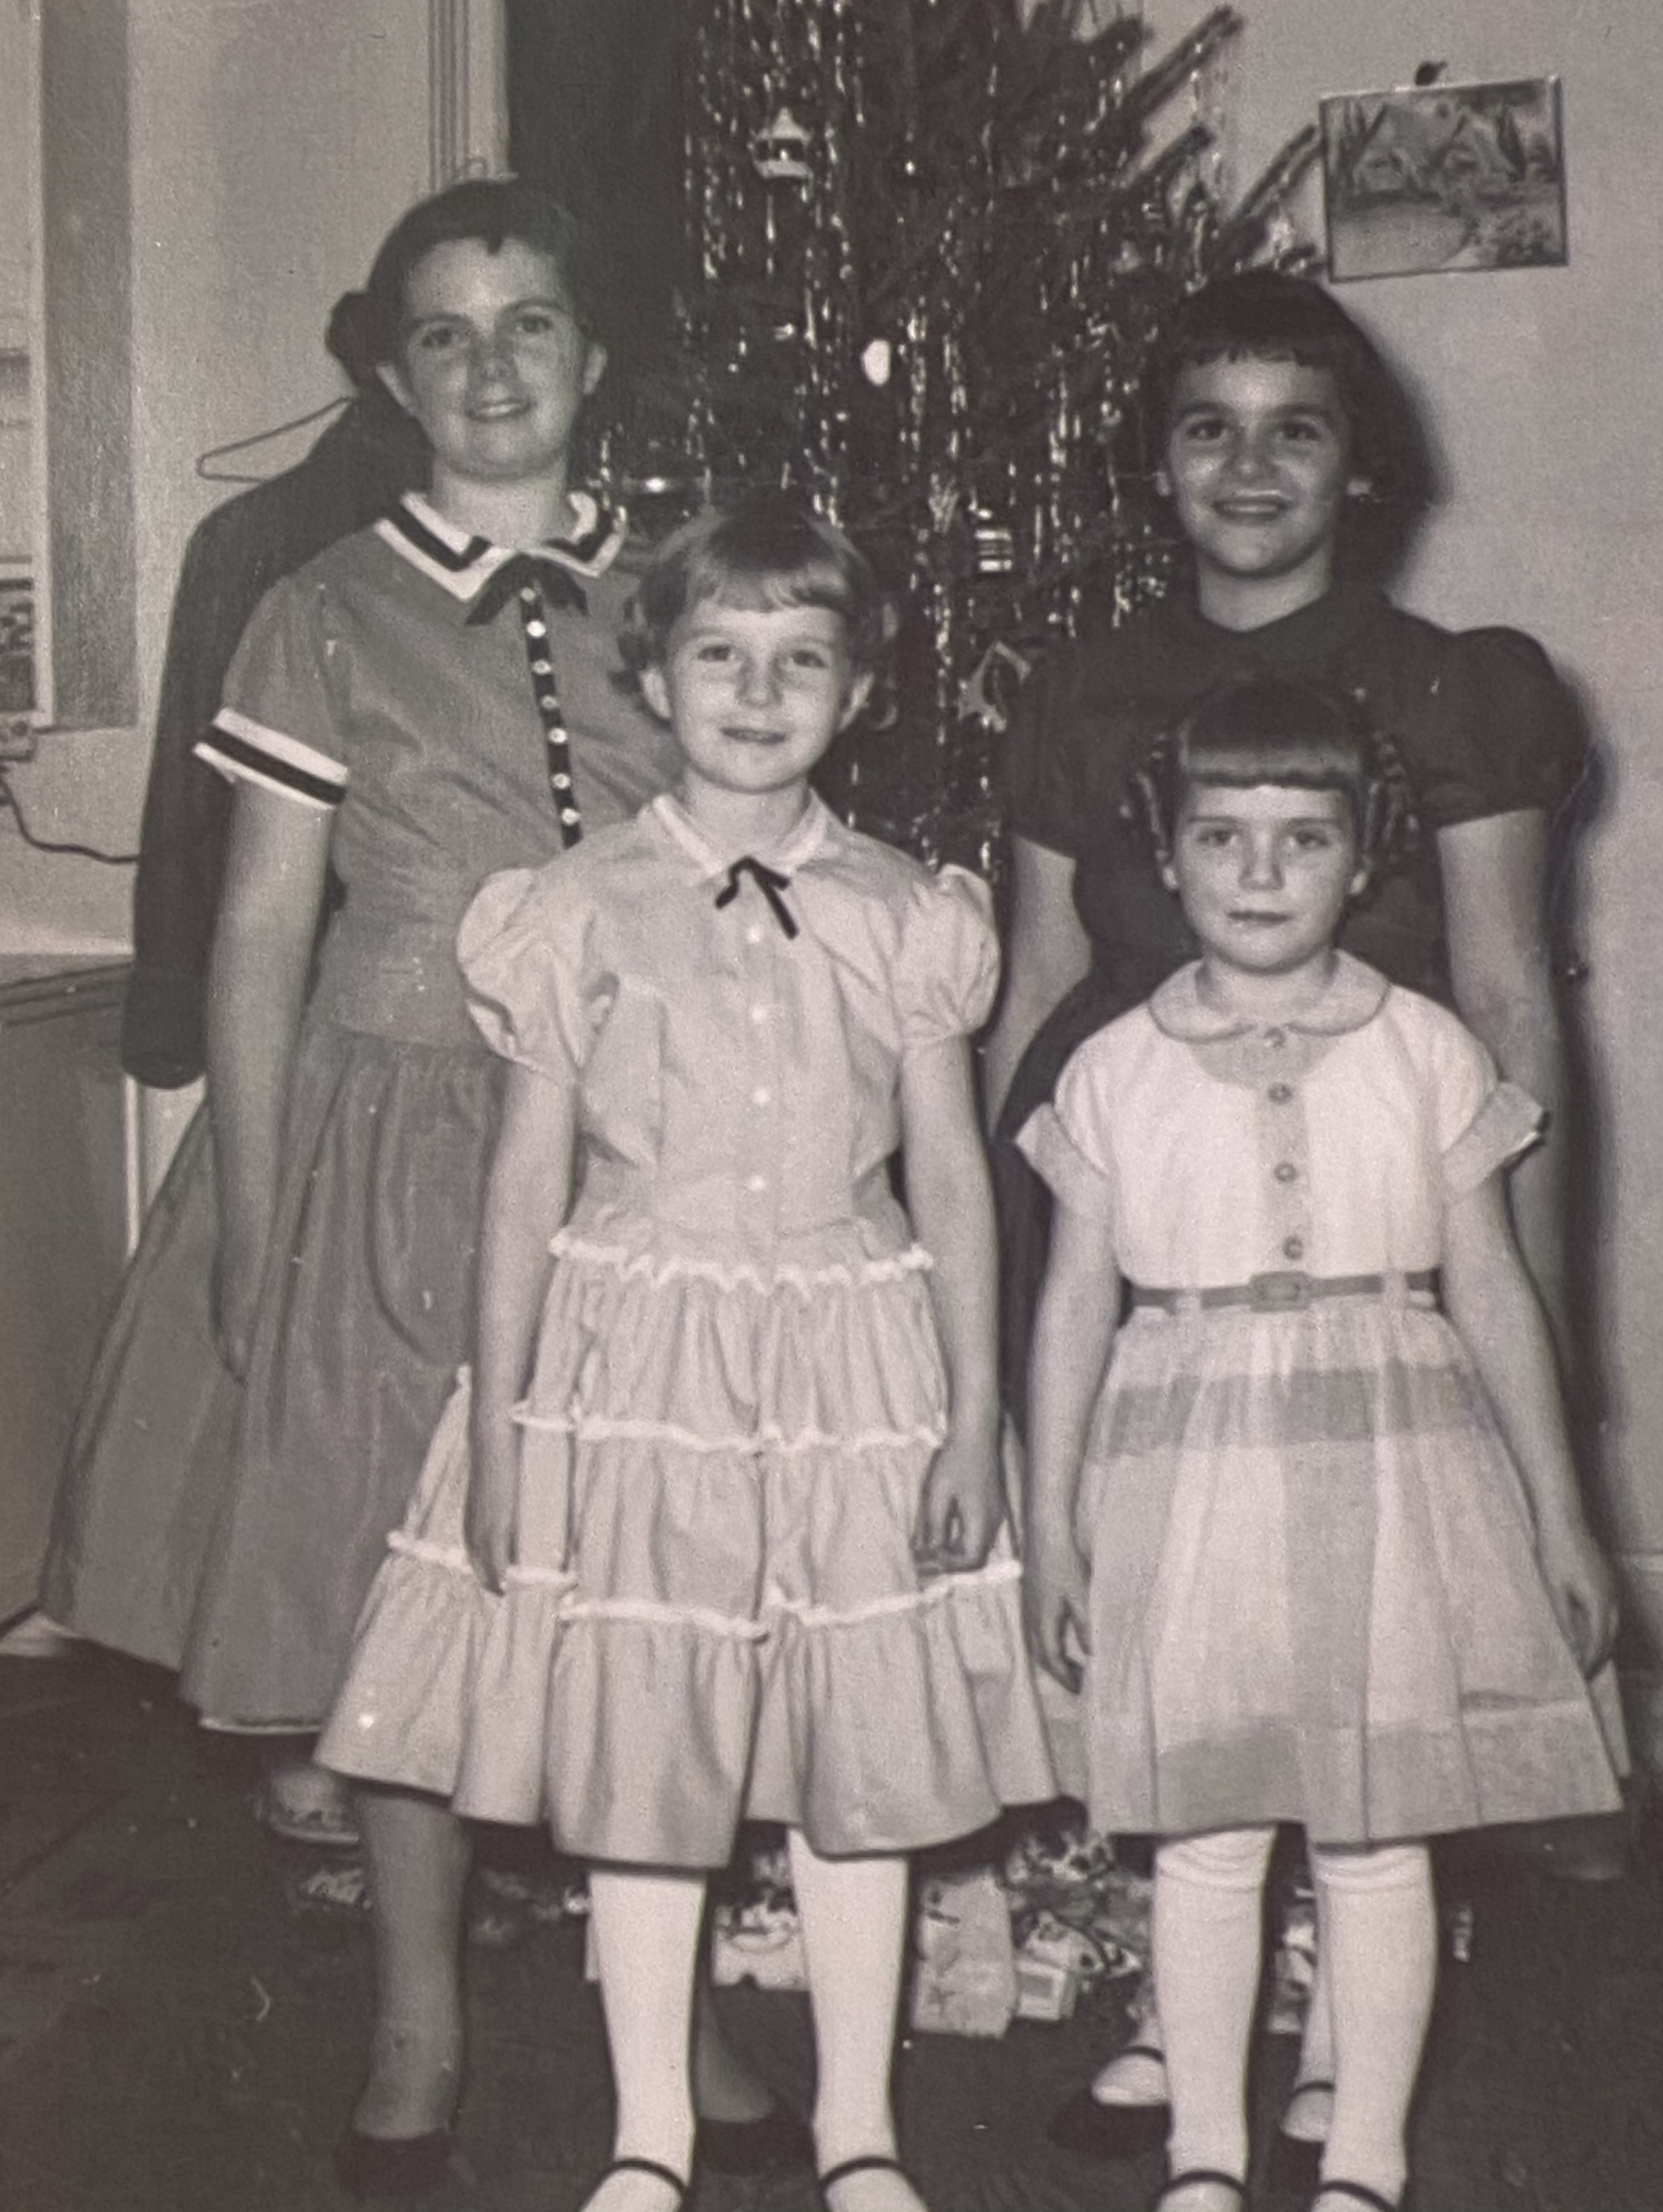
\includegraphics[width=0.55\linewidth,height=\textheight,keepaspectratio]{images/Akou26rt.jpg}

}

\caption{Myrtle Joyce, Alice, Hazel, and Bonnie; Christmas 1956}

\end{figure}%

\section{Notes}\label{notes-58}

Lila's last child, Larry, was adopted as a newborn. The couple that
adopted him, Chester and Gladys Peterson, had other biological children
and were very kind. They lived on a small farm not far from La Crosse.
My mother and her siblings knew about Larry; somehow, they found him
when I was a small child. I remember visiting the Peterson farm and
feeding carrots and apples to their Shetland ponies. Larry had a very
different childhood from his siblings.

Decades after she was adopted by an unrelated couple, my Aunt June
managed to get a copy of her original birth certificate and adoption
papers. Her father was not listed, but the file included summaries of
interviews that social workers conducted with Lila and Herman.

In the 1950s, social services in Wisconsin (foster care, welfare, food
stamps, etc.) were changing dramatically. After subsisting for many
years without support, I doubt Lila would have thought to ask for these
resources on her own. June told me about the house near Copeland Park.

For more information, see State Department of Public Welfare\footnote{\citeproc{ref-state1963a}{{``Social
  Work in Wisconsin: Helping You to Become Skilled in the Art of Helping
  Others''} (Madison, Wisconsin: State Department of Public Welfare,
  1963)}.}, Mark R. Rank\footnote{\citeproc{ref-rank1994a}{\emph{Living
  on the Edge: The Realities of Welfare in America} (New York: Columbia
  University Press, 1994)}.}, and Christina G. Villegas\footnote{\citeproc{ref-villegas2022a}{\emph{Foster
  Care in America: A Reference Handbook} (Oxford: Bloomsbury, 2022)}.}.

\bookmarksetup{startatroot}

\chapter{Chapter Fifty-Seven}\label{chapter-fifty-seven}

The seizures started in 1957. Lila fainted at work and couldn't be
revived; she was taken to the hospital in an ambulance. She half
expected to be told that she was pregnant again, even though she had
turned down all offers of sex for the last two years. At first, the
doctors were not sure what was wrong and told her they would need to run
some tests. In the end, they said her symptoms were probably from the
repeated pregnancies and toxemia; her kidneys were damaged, and her
blood pressure was out of control. Out of shame and misplaced loyalty,
she never told them about the pills from Merlin.

The hospital asked her for her next of kin. She didn't trust anyone and
didn't want to give them a name. Are your parents still alive? What
about a sibling? She never did tell them anything, but they found her
parents and brothers based on her last name. Reluctantly, she had
returned to using her maiden name after the divorce; she felt like she
had burned all of her bridges with the Schneiders.

By the time her father visited the hospital, she was in and out of
consciousness. The seizures were lasting longer and becoming more
frequent; Lila knew she was dying. Her father asked what she wanted to
do with the girls. In tears, she said, ``I want Hazel and Bonnie to stay
together.'' When she was unable to leave the hospital, the state had
sent them to live in the orphanage. In a flat tone that she could not
read, her father said, ``Izro will take them.'' The thought was
comforting. She had barely seen Izro in the last ten years, but she
trusted her more than Veda and her mother.

Myrtle Joyce was fourteen and looked so much like her father. Sometimes
in her dreams, Lila saw the men who had drifted in and out of her life:
Lloyd, Daniel, Herman, Jack. Aside from John and Alice, she had never
named the fathers on the children's birth certificates. The social
workers had asked repeatedly for names, but she didn't know what to tell
them. She didn't know the men who had raped her; even years later, it
gave her nightmares to think about the attack that led to Hazel's birth.

The damage to her kidneys caused her body and face to swell
uncontrollably. One day, a nurse gave her a mirror to hold while she
brushed her hair. Lila barely recognized her own image.

\section{Notes}\label{notes-59}

I know from my Aunt June that Lila had some time to plan what would
happen with her children after she died. There are photographs of her in
the hospital with her father and her son, Randy. I don't know if there
are others, but those are the photographs that I have seen. Lila was
very bloated and sitting in a wheelchair; compared to photos in her
twenties, she is barely recognizable.

For more information, see Frank Burnet Byrom\footnote{\citeproc{ref-byrom1969a}{\emph{The
  Hypertensive Vascular Crisis: An Experimental Study} (New York: Grune
  \& Stratton, 1969)}.}, Institute of Medicine\footnote{\citeproc{ref-institute2015a}{\emph{Dying
  in America: Improving Quality and Honoring Preferences Near the End of
  Life} (Washington, DC: National Academies Press, 2015)}.}, and Stephen
K. C. Ng et al.\footnote{\citeproc{ref-ng1993a}{{``Hypertension and the
  Risk of New-Onset Unprovoked Seizures,''} \emph{Neurology} 43, no. 2
  (1993): 425}.}

\bookmarksetup{startatroot}

\chapter{Epilogue}\label{epilogue}

When Lila died on October 7th, 1958, she was only thirty-six years old.
She never knew what was in the pills that Merlin gave her. During World
War II, Nazi troops were given enormous supplies of methamphetamine to
help them overcome exhaustion. When US troops entered the war, they were
given amphetamines for similar reasons. They found that it not only kept
them awake but also made them more focused, optimistic, and less hungry.
Both stimulants are highly addictive, increase users' heart rate and
blood pressure, and are known to cause pregnancy complications,
including pre-eclampsia (previously known as toxemia).

In the 1940s and 1950s, only five percent of white women in the United
States were single mothers. Social services like welfare were available,
but many women were either unaware of them or too ashamed (perhaps too
proud) to accept support from the government. When World War II ended,
many women---even if they were married and/or well-educated---were
frozen out of jobs that paid well enough to support a family.

At the end of her life, Lila thought the Schneiders had abandoned her,
but they had not. Despite the divorce, Herman claimed her body and
buried her as ``Lila Schneider'' in Neshonoc Cemetery just north of West
Salem. Four years after her husband died, Emma married Herman, and they
lived together until he died from a heart attack in 1973. Having met
because of Lila's children, they wanted to take Myrtle Joyce, Hazel, and
Bonnie, but the state would not allow it since they had too little
income and no legal claims. John lived with his father and Emma until
1963 when he was tragically killed in a tractor accident.

\begin{figure}[H]

{\centering 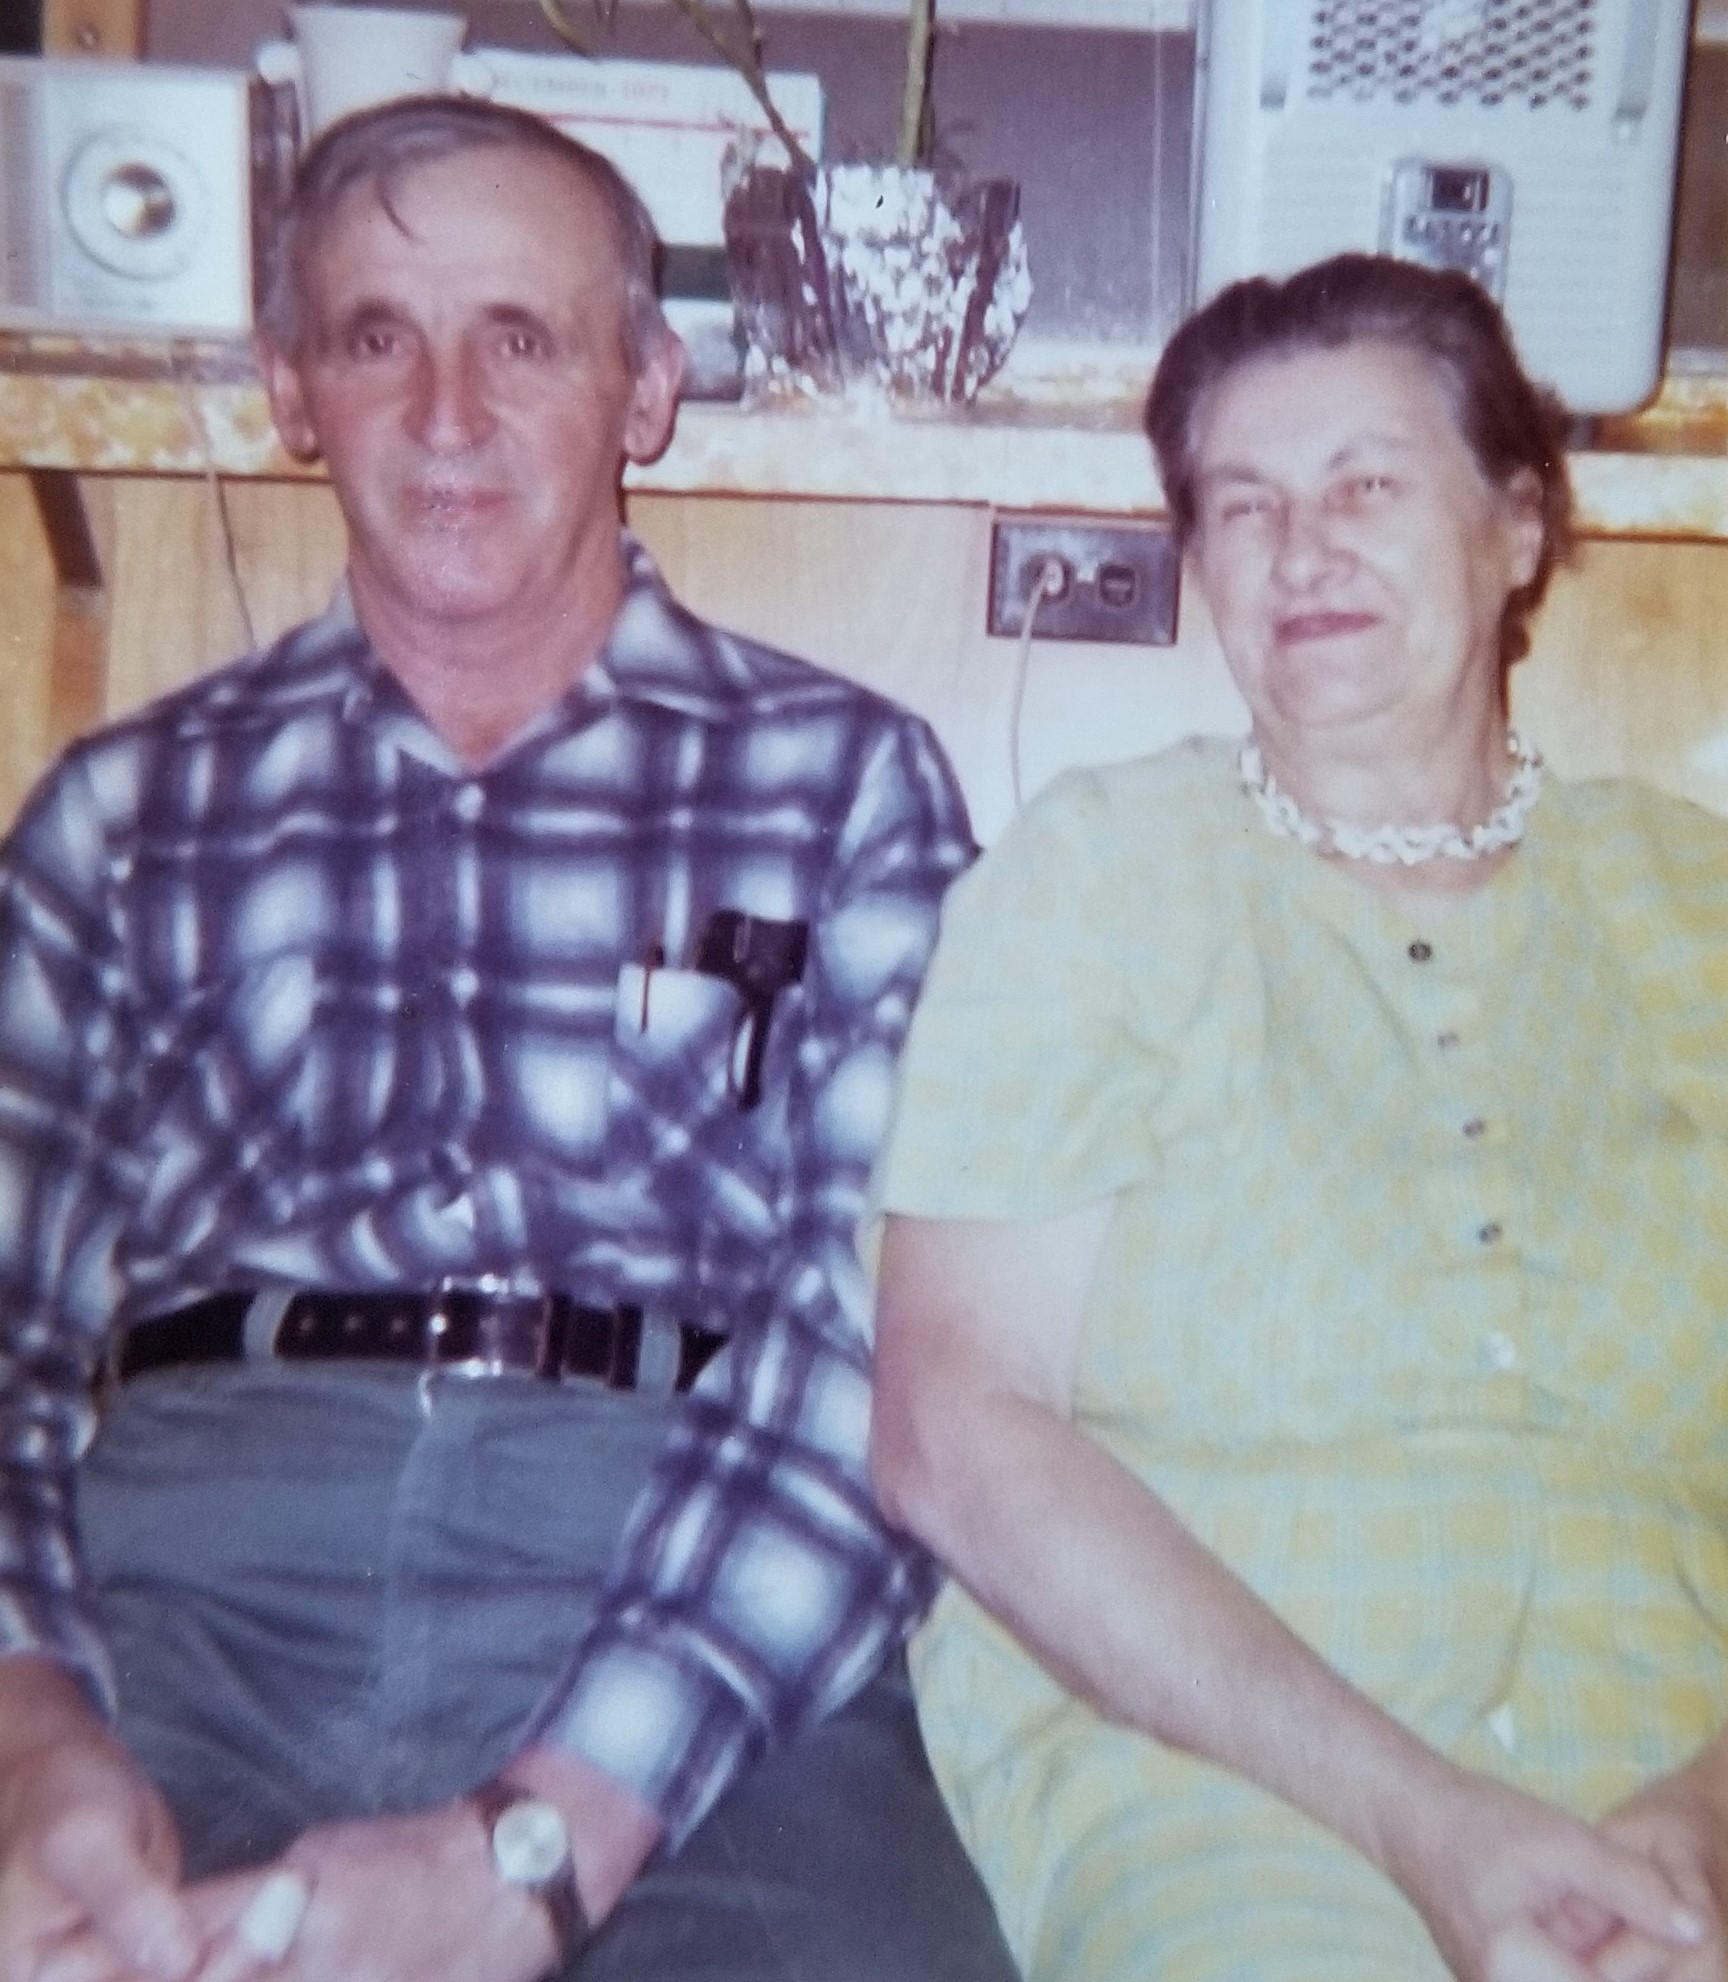
\includegraphics[width=0.55\linewidth,height=\textheight,keepaspectratio]{images/Akou27rt.jpg}

}

\caption{Herman and Emma, circa 1970}

\end{figure}%

Like her mother, Alice struggled to live with Herman on the farm. She
shuffled through various living arrangements including the orphanage and
foster homes. As a teenager, she went to live with Myrtle and Carl
Schneider and stayed with them during high school. Unlike her
half-brother Randy, they did not adopt her.

After Lila's death, Myrtle Joyce lived in foster homes until she aged
out of the system. In 1964 when she became engaged, the announcement in
the newspaper listed Herman Schneider as her father. Hazel and Bonnie
were sent to live with Izro's son, LeRoy; however, the arrangement did
not last. After LeRoy had a heart attack and his wife became pregnant
again, they decided to give custody back to the state, and the girls
were sent to an orphanage. They were adopted by an unrelated couple with
no biological children of their own. When the adoption papers were drawn
up, Hazel requested to change her name to June. As adults, all of the
siblings (including Larry) managed to find one another again and have
stayed in touch.

Both of Lila's parents outlived her by more than a decade, but none of
the Slabacks took custody of her children for more than a few months.
Veda died from cancer in 1971. She never went to nursing school and
never worked outside of the home after she was married to Red. Her
daughter, Patty, still visits Myrtle Joyce from time to time.

The effects of Lila's life continue to ripple through the generations;
she now has fifteen grandchildren and more than two dozen
great-grandchildren, including me and my children. I was never
encouraged to think of her as anything but a problem, but the process of
writing this book has reshaped what I think about her life. She tried so
hard to be herself and to live on her own terms, regardless of what
anyone thought about her. This is the kind of courage it takes to
disrupt generational patterns of dysfunction and discrimination. Lila
paid a steep price, but with her story out in the open, I choose to draw
from her strength and resilience.

\section{Notes}\label{notes-60}

I wrote this epilogue in 2020 and revised it in 2022. Although Myrtle
Joyce and my mother, Alice (Lila's second daughter) passed away in
February 2024, I have chosen not to revise the epilogue again. This
project has taught me just how much our stories outlive us.

For more information, see Magnus Chan, Jocelyn Joy Chan, and James M.
Wright\footnote{\citeproc{ref-chan2020a}{{``Effect of Amphetamines on
  Blood Pressure,''} \emph{Cochrane Database of Systematic Reviews}, no.
  12 (2020), \url{https://doi.org/10.1002/14651858.CD007896.pub3}}.},
Ray J. Defalque and Amos J. Wright\footnote{\citeproc{ref-defalque2011a}{{``Methamphetamine
  for Hitler's Germany: 1937 to 1945,''} \emph{Bulletin of Anesthesia
  History} 29, no. 2 (2011): 21--32,
  \url{https://doi.org/10.1016/S1522-8649(11)50016-2}}.}, Donald J.
Hernandez\footnote{\citeproc{ref-hernandez1993a}{\emph{America's
  Children: Resources from Family, Government, and the Economy} (New
  York: Russell Sage Foundation, 1993)}.}, Vorapong Phupong and Darigar
Darojn\footnote{\citeproc{ref-phupong2007a}{{``Amphetamine Abuse in
  Pregnancy: The Impact on Obstetric Outcome,''} \emph{Archives of
  Gynecology and Obstetrics} 276 (2007): 167--70,
  \url{https://doi.org/10.1007/s00404-007-0320-x}}.}, and Nicolas
Rasmussen\footnote{\citeproc{ref-rasmussen2015a}{{``Amphetamine-Type
  Stimulants: The Early History of Their Medical and Non-Medical
  Uses,''} in \emph{The Neuropsychiatric Complications of Stimulant
  Abuse}, ed. Pille Taba, Andrew Lees, and Katrin Sikk, vol. 120,
  International Review of Neurobiology, 2015, 9--25,
  \url{https://doi.org/10.1016/bs.irn.2015.02.001}}.}.

\bookmarksetup{startatroot}

\chapter*{Bibliography}\label{bibliography}
\addcontentsline{toc}{chapter}{Bibliography}

\markboth{Bibliography}{Bibliography}

\phantomsection\label{refs}
\begin{CSLReferences}{1}{0}
\bibitem[\citeproctext]{ref-adams2023a}
Adams, Jennifer L. \emph{An Autoethnography of Letter Writing and
Relationships Through Time: Finding Our Perfect Moon}. New York:
Routledge, 2023.

\bibitem[\citeproctext]{ref-agllias2016a}
Agllias, Kylie. \emph{Family Estrangement: A Matter of Perspective}.
Oxford: Taylor \& Francis, 2016.

\bibitem[\citeproctext]{ref-akou2024a}
Akou, Heather. \emph{On the Job: A History of American Work Uniforms}.
Oxford: Bloomsbury Academic, 2024.

\bibitem[\citeproctext]{ref-andreas2020a}
Andreas, Peter. \emph{Killers High: A History of War in Six Drugs}.
Oxford University Press, 2020.

\bibitem[\citeproctext]{ref-apple1986a}
Apple, Michael W. \emph{Teachers and Texts: A Political Economy of Class
and Gender Relations in Education}. New York: Routledge, 1986.

\bibitem[\citeproctext]{ref-apps2006a}
Apps, Jerry. \emph{When Chores Were Done: Boyhood Stories}. St. Paul:
MBI Publishing Company, 2006.

\bibitem[\citeproctext]{ref-babycenter2024a}
BabyCenter. {``Most Popular Baby Names of 1954.''} BabyCenter, 2024.
\url{https://www.babycenter.com/baby-names/most-popular/top-baby-names-1954}.

\bibitem[\citeproctext]{ref-bachner2008a}
Bachner, Evan. \emph{Making WAVES: Navy Women of World War II}. New
York: Harry N. Abrams, 2008.

\bibitem[\citeproctext]{ref-baeckstruxf6m2022a}
Baeckström, Ylva. \emph{Gender and Finance: Addressing Inequality in the
Financial Services Industry}. London: Taylor \& Francis, 2022.

\bibitem[\citeproctext]{ref-bailey1989a}
Bailey, Beth L. \emph{From Front Porch to Back Seat: Courtship in
Twentieth-Century America}. Baltimore: Johns Hopkins University Press,
1989.

\bibitem[\citeproctext]{ref-bair2016a}
Bair, Deidre. \emph{Al Capone: His Life, Legacy, and Legend}. New York:
Doubleday, 2016.

\bibitem[\citeproctext]{ref-Barillas2006a}
Barillas, William. \emph{The Midwestern Pastoral: Place and Landscape in
the Literature of the American Heartland}. Athens: Ohio University
Press, 2006.

\bibitem[\citeproctext]{ref-basile2005a}
Basile, Kathleen C. {``Sexual Violence in the Lives of Girls and
Women.''} In \emph{Handbook of Women, Stress, and Trauma}, edited by
Kathleen A. Kendall-Tackett, 101--22. New York: Brunner-Routledge, 2005.

\bibitem[\citeproctext]{ref-beekman2006a}
Beekman, Scott. \emph{Ringside: A History of Professional Wrestling in
America}. London: Bloomsbury, 2006.

\bibitem[\citeproctext]{ref-benson2007a}
Benson, Susan Porter. \emph{Household Accounts: Working-Class Family
Economies in the Interwar United States}. Ithaca: Cornell University
Press, 2007.

\bibitem[\citeproctext]{ref-bergland2011a}
Bergland, Betty A., and Lori Ann Lahlum, eds. \emph{Norwegian American
Women: Migration, Communities, and Identities}. St. Paul: Minnesota
Historical Society, 2011.

\bibitem[\citeproctext]{ref-blue2012a}
Blue, Ethan. \emph{Doing Time in the Depression: Everyday Life in Texas
and California Prisons}. New York University Press, 2012.

\bibitem[\citeproctext]{ref-bosworth2005a}
Bosworth, Mary, ed. \emph{Encyclopedia of Prisons \& Correctional
Facilities}. Thousand Oaks, California: SAGE Publications, 2005.

\bibitem[\citeproctext]{ref-bowen2014a}
Bowen, Ronda L. {``Birthday Parties.''} In \emph{The Social History of
the American Family: An Encyclopedia}, edited by Marilyn J. Coleman and
Lawrence H. Ganong, 115--16. New York: SAGE Publications, 2014.

\bibitem[\citeproctext]{ref-brewer2011a}
Brewer, Sarah, Shaoni Bhattacharya, Justine Davies, Sheena Meredith, and
Penny Preston. \emph{The Pregnant Body Book}. New York: DK Publishing,
2011.

\bibitem[\citeproctext]{ref-brooks2019a}
Brooks, Tim. \emph{The Blackface Minstrel Show in Mass Media: 20th
Century Performances on Radio, Records, Film and Television}. Jefferson,
North Carolina: McFarland, 2019.

\bibitem[\citeproctext]{ref-brumberg2010a}
Brumberg, Joan Jacobs. \emph{The Body Project: An Intimate History of
American Girls}. New York: Knopf Doubleday, 2010.

\bibitem[\citeproctext]{ref-budin2021a}
Budin, Stephanie Lynn. \emph{Freewomen, Patriarchal Authority, and the
Accusation of Prostitution}. London: Taylor \& Francis, 2021.

\bibitem[\citeproctext]{ref-burns-ardolino2007a}
Burns-Ardolino, Wendy A. \emph{Jiggle: (Re)shaping American Women}.
Lanham: Lexington Books, 2007.

\bibitem[\citeproctext]{ref-byrom1969a}
Byrom, Frank Burnet. \emph{The Hypertensive Vascular Crisis: An
Experimental Study}. New York: Grune \& Stratton, 1969.

\bibitem[\citeproctext]{ref-campbell2000a}
Campbell, Nancy. \emph{Using Women: Gender, Drug Policy, and Social
Justice}. New York: Routledge, 2000.

\bibitem[\citeproctext]{ref-cann2018a}
Cann, Candi K. \emph{Dying to Eat: Cross-Cultural Perspectives on Food,
Death, and the Afterlife}. Lexington: University Press of Kentucky,
2018.

\bibitem[\citeproctext]{ref-celani2011a}
Celani, David. \emph{Leaving Home: The Art of Separating from Your
Difficult Family}. New York: Columbia University Press, 2011.

\bibitem[\citeproctext]{ref-celello2009a}
Celello, Kristin. \emph{Making Marriages Work: A History of Marriage and
Divorce in the Twentieth-Century United States}. Chapel Hill: University
of North Carolina Press, 2009.

\bibitem[\citeproctext]{ref-chan2020a}
Chan, Magnus, Jocelyn Joy Chan, and James M. Wright. {``Effect of
Amphetamines on Blood Pressure.''} \emph{Cochrane Database of Systematic
Reviews}, no. 12 (2020).
\url{https://doi.org/10.1002/14651858.CD007896.pub3}.

\bibitem[\citeproctext]{ref-chapman2021a}
Chapman, Fern Schumer. \emph{Brothers, Sisters, Strangers: Sibling
Estrangement and the Road to Reconciliation}. New York: Penguin
Publishing, 2021.

\bibitem[\citeproctext]{ref-cherlin2014a}
Cherlin, Andrew J. \emph{Labor's Love Lost: The Rise and Fall of the
Working-Class Family in America}. New York: Russell Sage Foundation,
2014.

\bibitem[\citeproctext]{ref-clemente2014a}
Clemente, Deirdre. \emph{Dress Casual: How College Students Redefined
American Style}. Chapel Hill: University of North Carolina Press, 2014.

\bibitem[\citeproctext]{ref-cobble1992a}
Cobble, Dorothy. \emph{Dishing It Out: Waitresses and Their Unions in
the Twentieth Century}. Champaign: University of Illinois Press, 1992.

\bibitem[\citeproctext]{ref-cobble2004a}
Cobble, Dorothy Sue. \emph{The Other Women's Movement: Workplace Justice
and Social Rights in Modern America}. Princeton University Press, 2004.

\bibitem[\citeproctext]{ref-collier2010a}
Collier, Aine. \emph{The Humble Little Condom: A History}. Amherst:
Prometheus, 2010.

\bibitem[\citeproctext]{ref-cray1999a}
Cray, Ed. \emph{The Erotic Muse: American Bawdy Songs}. Champaign:
University of Illinois Press, 1999.

\bibitem[\citeproctext]{ref-current1977a}
Current, Richard Nelson. \emph{Wisconsin: A History}. 1977. Reprint,
{Urbana and Chicago}: University of Illinois Press, 2001.

\bibitem[\citeproctext]{ref-dank2018a}
Dank, Barry M., and Roberto Refinetti, eds. \emph{Sex Work and Sex
Workers}. Oxford: Taylor \& Francis, 2018.

\bibitem[\citeproctext]{ref-davis-floyd1992a}
Davis-Floyd, Robbie. \emph{Birth as an American Rite of Passage}.
Berkeley: University of California Press, 1992.

\bibitem[\citeproctext]{ref-defalque2011a}
Defalque, Ray J., and Amos J. Wright. {``Methamphetamine for Hitler's
Germany: 1937 to 1945.''} \emph{Bulletin of Anesthesia History} 29, no.
2 (2011): 21--32. \url{https://doi.org/10.1016/S1522-8649(11)50016-2}.

\bibitem[\citeproctext]{ref-devries2001a}
DeVries, Raymond, Sirpa Wrede, Edwin van Teijlingen, and Cecilia Benoit,
eds. \emph{Birth by Design: Pregnancy, Maternity Care, and Midwifery in
North America and Europe}. New York: Routledge, 2001.

\bibitem[\citeproctext]{ref-doka2014a}
Doka, Kenneth J., ed. \emph{Children Mourning, Mourning Children}.
Abingdon, United Kingdom: Taylor \& Francis, 2014.

\bibitem[\citeproctext]{ref-dolan2010a}
Dolan, Jay P. \emph{The Irish Americans: A History}. New York:
Bloomsbury USA, 2010.

\bibitem[\citeproctext]{ref-draeger2012a}
Draeger, Jim, and Mark Speltz. \emph{Bottoms up: A Toast to Wisconsin's
Historic Bars and Breweries}. Madison: Wisconsin Historical Society
Press, 2012.

\bibitem[\citeproctext]{ref-elliott2014a}
Elliott, Julian G., and Elena L. Grigorenko. \emph{The Dyslexia Debate}.
Cambridge University Press, 2014.

\bibitem[\citeproctext]{ref-emmet1950a}
Emmet, Boris, and John E. Jeuck. \emph{Catalogues and Counters: A
History of Sears, Roebuck and Company}. University of Chicago Press,
1950.

\bibitem[\citeproctext]{ref-fcconline2024a}
Family \& Children's Center. {``Our History.''} Family \& Children's
Center, 2024. \url{https://www.fcconline.org/our-history/}.

\bibitem[\citeproctext]{ref-farrell-beck2007a}
Farrell-Beck, Jane, and Jean Parsons. \emph{{20\(^{th}\)-Century} Dress
in the United States}. New York: Fairchild, 2007.

\bibitem[\citeproctext]{ref-fwha1997a}
Federal Highway Administration Office of Highway Information Management.
{``Highway Statistics Summary to 1995.''} Washington, DC: Federal
Highway Administration, 1997.
\url{https://www.fhwa.dot.gov/ohim/summary95/dl230.pdf}.

\bibitem[\citeproctext]{ref-fehribach2023a}
Fehribach, Paul. \emph{Midwestern Food: A Chef's Guide to the Surprising
History of a Great American Cuisine, with More Than 100 Tasty Recipes}.
University of Chicago Press, 2023.

\bibitem[\citeproctext]{ref-feldstein2018a}
Feldstein, Ruth. \emph{Motherhood in Black and White: Race and Sex in
American Liberalism, 1930--1965}. Ithaca: Cornell University Press,
2018.

\bibitem[\citeproctext]{ref-fessler2006a}
Fessler, Ann. \emph{The Girls Who Went Away: The Hidden History of Women
Who Surrendered Children for Adoption in the Decades Before Roe v.
Wade}. New York: Penguin Group, 2006.
\url{https://www.thegirlswhowentaway.com/}.

\bibitem[\citeproctext]{ref-fine2008a}
Fine, Gary Alan. \emph{Kitchens: The Culture of Restaurant Work}.
Berkeley: University of California Press, 2008.

\bibitem[\citeproctext]{ref-finkbeiner2012a}
Finkbeiner, Ann K. \emph{After the Death of a Child: Living with Loss
Through the Years}. New York: Free Press, 2012.

\bibitem[\citeproctext]{ref-fitzgerald1920a}
Fitzgerald, F. Scott. {``Bernice Bobs Her Hair.''} \emph{The Saturday
Evening Post}, 1920.
\url{https://public.wsu.edu/~campbelld/engl494/bernicebobs.pdf}.

\bibitem[\citeproctext]{ref-ford2016a}
Ford, Gilbert. \emph{The Marvelous Thing That Came from a Spring: The
Accidental Invention of the Toy That Swept the Nation}. New York:
Atheneum Books for Young Readers, 2016.

\bibitem[\citeproctext]{ref-foster1918a}
Foster, Leslie Everett. \emph{Secrets of Dry Cleaning}. York: York Blank
Book Company, 1918.

\bibitem[\citeproctext]{ref-fournier2008a}
Fournier, Linda M. \emph{Fort McCoy}. Mount Pleasant: Arcadia
Publishing, 2008.

\bibitem[\citeproctext]{ref-freedman2005a}
Freedman, Russell. \emph{Children of the Great Depression}. New York:
Clarion Books, 2005.

\bibitem[\citeproctext]{ref-mcgarvie2003a}
Friedman, Lawrence Jacob, and Mark Douglas McGarvie, eds. \emph{Charity,
Philanthropy, and Civility in American History}. Cambridge University
Press, 2003.

\bibitem[\citeproctext]{ref-friedman2003a}
Friedman, Lawrence J., and Mark D. McGarvie, eds. \emph{Charity,
Philanthropy, and Civility in American History}. Cambridge University
Press, 2003.

\bibitem[\citeproctext]{ref-gallagher2016a}
Gallagher, Winifred. \emph{How the Post Office Created America: A
History}. New York: Penguin Publishing, 2016.

\bibitem[\citeproctext]{ref-garland1917a}
Garland, Hamlin. \emph{A Son of the Middle Border}. New York: Macmillan
Company, 1917.

\bibitem[\citeproctext]{ref-glaser2021a}
Glaser, Gabrielle. \emph{American Baby: A Mother, a Child, and the
Secret History of Adoption}. New York: Penguin Publishing, 2021.

\bibitem[\citeproctext]{ref-glitre2013a}
Glitre, Kathrina. \emph{Hollywood Romantic Comedy: States of Union,
1934--1965}. Manchester University Press, 2013.

\bibitem[\citeproctext]{ref-goldin2021a}
Goldin, Claudia. \emph{Career and Family: Women's Century-Long Journey
Toward Equity}. Princeton University Press, 2021.

\bibitem[\citeproctext]{ref-goldman2013a}
Goldman, Kay. \emph{Dressing Modern Maternity: The Frankfurt Sisters of
Dallas and the Page Boy Label}. Lubbock: Texas Tech University Press,
2013.

\bibitem[\citeproctext]{ref-goldstein2012a}
Goldstein, Carolyn M. \emph{Creating Consumers: Home Economists in
Twentieth-Century America}. Chapel Hill: University of North Carolina
Press, 2012.

\bibitem[\citeproctext]{ref-greenholt2023a}
Greenholt, Carol. \emph{Tales of a Dry Cleaner}. Meadville: Christian
Faith Publishing, 2023.

\bibitem[\citeproctext]{ref-gregory2005a}
Gregory, James Noble. \emph{The Southern Diaspora: How the Great
Migrations of Black and White Southerners Transformed America}. Chapel
Hill: University of North Carolina Press, 2005.

\bibitem[\citeproctext]{ref-greif2015a}
Greif, Geoffrey L., and Michael E. Woolley. \emph{Adult Sibling
Relationships}. New York: Columbia University Press, 2015.

\bibitem[\citeproctext]{ref-grinspoon1975a}
Grinspoon, Lester, and Peter Hedblom. \emph{The Speed Culture:
Amphetamine Use and Abuse in America}. Cambridge: Harvard University
Press, 1975.

\bibitem[\citeproctext]{ref-mississippi1914a}
{``Guide to the Mississippi Valley Public Service Company Records, MSS
028.''} La Crosse Public Library Archives, 1914-\/-1942.
\url{https://archives.lacrosselibrary.org/collections/businesses/mss028/}.

\bibitem[\citeproctext]{ref-gup2010a}
Gup, Ted. \emph{A Secret Gift: How One Man's Kindness---and a Trove of
Letters---Revealed the Hidden History of the Great Depression}. New
York: Penguin Publishing, 2010.

\bibitem[\citeproctext]{ref-hall2019a}
Hall, Lauren K. \emph{The Medicalization of Birth and Death}. Baltimore:
Johns Hopkins University Press, 2019.

\bibitem[\citeproctext]{ref-hark2007a}
Hark, Ina Rae, ed. \emph{American Cinema of the 1930s: Themes and
Variations}. New Brunswick, New Jersey: Rutgers University Press, 2007.

\bibitem[\citeproctext]{ref-harris2018a}
Harris, Chelsia. \emph{Hannah Visits Nana in the Nursing Home}.
Meadville: Christian Faith Publishing, 2018.

\bibitem[\citeproctext]{ref-heap2009a}
Heap, Chad. \emph{Slumming: Sexual and Racial Encounters in American
Nightlife, 1885--1940}. University of Chicago Press, 2009.

\bibitem[\citeproctext]{ref-heineman2011a}
Heineman, Elizabeth D., ed. \emph{Sexual Violence in Conflict Zones:
From the Ancient World to the Era of Human Rights}. University of
Pennsylvania Press, 2011.

\bibitem[\citeproctext]{ref-helgren2022a}
Helgren, Jennifer. \emph{The Camp Fire Girls: Gender, Race, and American
Girlhood, 1910--1980}. Lincoln: University of Nebraska Press, 2022.

\bibitem[\citeproctext]{ref-henderson2001a}
Henderson, Sylvia M. {``Baumkuchen.''} \emph{Gastronomica} 1, no. 2
(2001): 90--92.

\bibitem[\citeproctext]{ref-herman1992a}
Herman, Judith Lewis. \emph{Trauma and Recovery: The Aftermath of
Violence---from Domestic Abuse to Political Terror}. New York: Basic
Books, 1992.

\bibitem[\citeproctext]{ref-hernandez1993a}
Hernandez, Donald J. \emph{America's Children: Resources from Family,
Government, and the Economy}. New York: Russell Sage Foundation, 1993.

\bibitem[\citeproctext]{ref-hilmes1997a}
Hilmes, Michele. \emph{Radio Voices: American Broadcasting, 1922--1952}.
Minneapolis: University of Minnesota Press, 1997.

\bibitem[\citeproctext]{ref-hinshelwood1917a}
Hinshelwood, James. \emph{Congenital Word-Blindness}. London: H. K.
Lewis \& Co. Ltd., 1917.

\bibitem[\citeproctext]{ref-hoffmann2004a}
Hoffmann, Frank, Frederick J. Augustyn Jr., and Martin J. Manning.
\emph{Dictionary of Toys and Games in American Popular Culture}.
Philadelphia: Haworth Press, 2004.

\bibitem[\citeproctext]{ref-hogan1999a}
Hogan, David G. \emph{Selling 'Em by the Sack: White Castle and the
Creation of American Food}. New York University Press, 1999.

\bibitem[\citeproctext]{ref-howard2008a}
Howard, Vicki. \emph{Brides, Inc.: American Weddings and the Business of
Tradition}. Philadelphia: University of Pennsylvania Press, 2008.

\bibitem[\citeproctext]{ref-howell2015a}
Howell, James C. \emph{The History of Street Gangs in the United States:
Their Origins and Transformations}. Lanham, Maryland: Lexington Books,
2015.

\bibitem[\citeproctext]{ref-illouz2023a}
Illouz, Eva. \emph{Consuming the Romantic Utopia: Love and Cultural
Contradictions of Capitalism}. Berkeley: University of California Press,
2023.

\bibitem[\citeproctext]{ref-institute2015a}
Institute of Medicine. \emph{Dying in America: Improving Quality and
Honoring Preferences Near the End of Life}. Washington, DC: National
Academies Press, 2015.

\bibitem[\citeproctext]{ref-isenberg2021a}
Isenberg, Sheila. \emph{Women Who Love Men Who Kill: 35 True Stories of
Prison Passion}. New York: Diversion Books, 2021.

\bibitem[\citeproctext]{ref-jellison2008a}
Jellison, Katherine. \emph{It's Our Day: America's Love Affair with the
White Wedding, 1945--2005}. Lawrence: University Press of Kansas, 2008.

\bibitem[\citeproctext]{ref-joiner2009a}
Joiner, Thomas. \emph{Why People Die by Suicide}. Cambridge: Harvard
University Press, 2009.

\bibitem[\citeproctext]{ref-joselit2014a}
Joselit, Jenna Weissman. \emph{A Perfect Fit: Clothes, Character, and
the Promise of America}. New York: Henry Holt; Company, 2014.

\bibitem[\citeproctext]{ref-kahane1986a}
Kahane, Charles J. {``An Evaluation of Child Passenger Safety: The
Effectiveness and Benefits of Safety Seats.''} Washington, DC: National
Highway Traffic Safety Administration, 1986.

\bibitem[\citeproctext]{ref-katz2012a}
Katz, Nikki. \emph{The Book of Card Games: The Complete Rules to the
Classics, Family Favorites, and Forgotten Games}. New York: Simon;
Schuster, 2012.

\bibitem[\citeproctext]{ref-kearns1999a}
Kearns, Ellen C., and Monica Gallagher, eds. \emph{The Fair Labor
Standards Act}. Washington, DC: Bureau of National Affairs, 1999.

\bibitem[\citeproctext]{ref-keesecker1934a}
Keesecker, Ward Wilbur. \emph{The Legal Status of Married Women
Teachers}. Washington, DC: US Department of the Interior Office of
Education, 1934.

\bibitem[\citeproctext]{ref-kelly2017a}
Kelly, Kate. {``Dick and Jane: Story of These Early Readers,''} June 2,
2017.
\url{https://americacomesalive.com/dick-and-jane-story-of-these-early-readers/}.

\bibitem[\citeproctext]{ref-kennedy1984a}
Kennedy, Peter. \emph{Folksongs of Britain and Ireland}. San Francisco:
Oak Publications, 1984.

\bibitem[\citeproctext]{ref-king2001a}
King, Larry. \emph{Love Stories of World War II}. New York: Crown
Publishing, 2001.

\bibitem[\citeproctext]{ref-kunzel1993a}
Kunzel, Regina G. \emph{Fallen Women, Problem Girls: Unmarried Mothers
and the Professionalization of Social Work, 1890--1945}. New Haven:
Yale, 1993.

\bibitem[\citeproctext]{ref-lacrosselibrary2022a}
La Crosse Public Library Archives \& Local History Department. {``The
Way It Was: Roosevelt School, Circa 1931,''} May 22, 2022.
\url{https://lacrossetribune.com/the-way-it-was-roosevelt-school-circa-1931/article_66e6c3d6-d9fa-11ec-b99f-83bfbe095d45.html}.

\bibitem[\citeproctext]{ref-lamphier2017a}
Lamphier, Peg A., and Rosanne Welch, eds. \emph{Women in American
History: A Social, Political, and Cultural Encyclopedia and Document
Collection}. Oxford: Bloomsbury, 2017.

\bibitem[\citeproctext]{ref-leavitt2016a}
Leavitt, Judith Walzer. \emph{Brought to Bed: Childbearing in America,
1750--1950}. Oxford University Press, 2016.

\bibitem[\citeproctext]{ref-leonard2019a}
Leonard, Samanta. \emph{Groomed: Shining a Light on the Unheard
Narrative of Childhood Sexual Assault}. Washington, DC: New Degree
Press, 2019.

\bibitem[\citeproctext]{ref-licht200a}
Licht, Walter. \emph{Getting Work: Philadelphia, 1840--1950}.
Philadelphia: University of Pennsylvania Press, 2000.

\bibitem[\citeproctext]{ref-lilly2007a}
Lilly, J. Robert. \emph{Taken by Force: Rape and American GIs in Europe
During World War II}. London: Palgrave Macmillan, 2007.

\bibitem[\citeproctext]{ref-loewen2018a}
Loewen, James W. \emph{Sundown Town: A Hidden Dimension of American
Racism}. New York: New Press, 2018.

\bibitem[\citeproctext]{ref-lutz2001a}
Lutz, Catherine. \emph{Homefront: A Military City and the American
Twentieth Century}. Boston: Beacon Press, 2001.

\bibitem[\citeproctext]{ref-march2015a}
March, Rick, and Dick Blau. \emph{Polka Heartland: Why the Midwest Loves
to Polka}. Madison: Wisconsin Historical Society Press, 2015.

\bibitem[\citeproctext]{ref-mcbee2000a}
McBee, Randy D. \emph{Dance Hall Days: Intimacy and Leisure Among
Working-Class Immigrants in the United States}. New York: New York
University Press, 2000.

\bibitem[\citeproctext]{ref-mcelvaine2009a}
McElvaine, Robert S., ed. \emph{Down and Out in the Great Depression:
Letters from the Forgotten Man}. Chapel Hill: University of North
Carolina Press, 2009.

\bibitem[\citeproctext]{ref-miller2007a}
Miller, Susan. \emph{Vintage Feed Sacks: Fabric from the Farm}.
Lancaster, Pennsylvania: Schiffer Publishing, 2007.

\bibitem[\citeproctext]{ref-mjagkij1997a}
Mjagkij, Nina, and Margaret Spratt, eds. \emph{Men and Women Adrift: The
YMCA and the YWCA in the City}. New York University Press, 1997.

\bibitem[\citeproctext]{ref-modh2011a}
Modh, Carin, Ingela Lundgren, and Ingegerd Bergbom. {``First Time
Pregnant Women's Experiences in Early Pregnancy.''} \emph{International
Journal of Qualitative Studies in Health and Well-Being} 6, no. 2
(2011). \url{https://doi.org/10.3402/qhw.v6i2.5600}.

\bibitem[\citeproctext]{ref-morser2003a}
Morser, Eric J. {``Manufacturing Pioneers: Commerce, Government, and
Manhood in La Crosse, Wisconsin, 1840-1900.''} PhD Dissertation,
University of Wisconsin, 2003.

\bibitem[\citeproctext]{ref-mullen2017a}
Mullen, Lincoln A. \emph{The Chance of Salvation: A History of
Conversion in America}. Cambridge: Harvard University Press, 2017.

\bibitem[\citeproctext]{ref-nader1965a}
Nader, Ralph. \emph{Unsafe at Any Speed: The Designed-in Dangers of the
American Automobile}. New York: Grossman Publishers, 1965.

\bibitem[\citeproctext]{ref-nelson1954a}
Nelson, Lowry. \emph{American Farm Life}. Cambridge: Harvard University
Press, 1954.

\bibitem[\citeproctext]{ref-ng1993a}
Ng, Stephen K. C., W. Allen Hauser, John C. M. Brust, and Mervyn Susser.
{``Hypertension and the Risk of New-Onset Unprovoked Seizures.''}
\emph{Neurology} 43, no. 2 (1993): 425.

\bibitem[\citeproctext]{ref-nolen1911a}
Nolen, John. \emph{The Making of a Park System in La Crosse}. La Crosse:
The Inland Printing Company, 1911.

\bibitem[\citeproctext]{ref-norton2011a}
Norton, Peter D. \emph{Fighting Traffic: The Dawn of the Motor Age in
the American City}. Boston: MIT Press, 2011.

\bibitem[\citeproctext]{ref-oldenglishcrackers2024a}
Olde English Crackers. {``How to Make Christmas Crackers: A DIY
Guide.''} Olde English Crackers, 2024.
\url{https://www.oldenglishcrackers.com/how-to-make-christmas-crackers/}.

\bibitem[\citeproctext]{ref-oshinsky2005a}
Oshinsky, David M. \emph{Polio: An American Story}. Oxford University
Press, 2005.

\bibitem[\citeproctext]{ref-ottenheimer1996a}
Ottenheimer, Martin. \emph{Forbidden Relatives: The American Myth of
Cousin Marriage}. Champaign: University of Illinois Press, 1996.

\bibitem[\citeproctext]{ref-palmer2010a}
Palmer, Phyllis. \emph{Domesticity and Dirt: Housewives and Domestic
Servants in the United States, 1920--1945}. Philadelphia: Temple
University Press, 2010.

\bibitem[\citeproctext]{ref-paules1991a}
Paules, Greta Foff. \emph{Dishing It Out: Power and Resistance Among
Waitresses in a New Jersey Restaurant}. Philadelphia: Temple University
Press, 1991.

\bibitem[\citeproctext]{ref-perel2017a}
Perel, Esther. \emph{The State of Affairs: Rethinking Infidelity}. New
York: HarperCollins Publishers, 2017.

\bibitem[\citeproctext]{ref-peters2023a}
Peters, Lauren Downing. \emph{Fashion Before Plus-Size: Bodies, Bias,
and the Birth of an Industry}. Oxford: Bloomsbury Academic, 2023.

\bibitem[\citeproctext]{ref-peterson1948a}
Peterson, Alvin Martin. \emph{Palisades and Coulees: The Scenic
Mississippi Valley from Prairie Du Chien to Red Wing}. Onalaska: Modern
Print Company, 1948.

\bibitem[\citeproctext]{ref-pfeifer2014a}
Pfeifer, Susan K., and Marvin B. Sussman. \emph{Families:
Intergenerational and Generational Connections}. New York: Routledge,
2014.

\bibitem[\citeproctext]{ref-cutright1972a}
Phillips, Cutright. {``Historical and Contemporary Trends in
Illegitimacy.''} \emph{Archives of Sexual Behavior} 2, no. 2 (1972):
97--118.

\bibitem[\citeproctext]{ref-phupong2007a}
Phupong, Vorapong, and Darigar Darojn. {``Amphetamine Abuse in
Pregnancy: The Impact on Obstetric Outcome.''} \emph{Archives of
Gynecology and Obstetrics} 276 (2007): 167--70.
\url{https://doi.org/10.1007/s00404-007-0320-x}.

\bibitem[\citeproctext]{ref-plunkett-powell2014a}
Plunkett-Powell, Karen. \emph{Remembering Woolworth's: A Nostalgic
History of the World's Most Famous Five-and-Dime}. New York: St.
Martin's Publishing Group, 2014.

\bibitem[\citeproctext]{ref-polakow1994a}
Polakow, Valerie. \emph{Lives on the Edge: Single Mothers and Their
Children in the Other America}. University of Chicago Press, 1994.

\bibitem[\citeproctext]{ref-rank1994a}
Rank, Mark R. \emph{Living on the Edge: The Realities of Welfare in
America}. New York: Columbia University Press, 1994.

\bibitem[\citeproctext]{ref-ranney1998a}
Ranney, Joseph A. {``Traditional Values and No-Fault Divorce.''}
Wisconsin Court System, 1998.
\url{https://www.wicourts.gov/courts/history/article45.htm}.

\bibitem[\citeproctext]{ref-rasmussen2008a}
Rasmussen, Nicolas. {``America's First Amphetamine Epidemic,
1929--1971.''} \emph{American Journal of Public Health} 98, no. 6
(2008): 974--85.

\bibitem[\citeproctext]{ref-rasmussen2015a}
Rasmussen, Nicolas. {``Amphetamine-Type Stimulants: The Early History of
Their Medical and Non-Medical Uses.''} In \emph{The Neuropsychiatric
Complications of Stimulant Abuse}, edited by Pille Taba, Andrew Lees,
and Katrin Sikk, 120:9--25. International Review of Neurobiology, 2015.
\url{https://doi.org/10.1016/bs.irn.2015.02.001}.

\bibitem[\citeproctext]{ref-ray2020a}
Ray, Robert B. \emph{A Certain Tendency of the Hollywood Cinema,
1930--1980}. Princeton University Press, 2020.

\bibitem[\citeproctext]{ref-reagan2022a}
Reagan, Leslie J. \emph{When Abortion Was a Crime: Women, Medicine, and
Law in the United States, 1867--1973}. Berkeley: University of
California Press, 2022.

\bibitem[\citeproctext]{ref-reef2005a}
Reef, Catherine. \emph{Alone in the World: Orphans and Orphanages in
America}. New York: Clarion Books, 2005.

\bibitem[\citeproctext]{ref-regis2013a}
Regis, Pamela. \emph{A Natural History of the Romance Novel}.
Philadelphia: University of Pennsylvania Press, 2013.

\bibitem[\citeproctext]{ref-riley2013a}
Riley, Naomi Schaefer. \emph{'Til Faith Do Us Part: How Interfaith
Marriage Is Transforming America}. Oxford University Press, 2013.

\bibitem[\citeproctext]{ref-riney-kehrberg2016a}
Riney-Kehrberg, Pamela, ed. \emph{The Routledge History of Rural
America}. New York: Routledge, 2016.

\bibitem[\citeproctext]{ref-rose2012a}
Rose, Kenneth. \emph{Myth and the Greatest Generation: A Social History
of Americans in World War II}. New York: Routledge, 2012.

\bibitem[\citeproctext]{ref-rosenfeld2017a}
Rosenfeld, Rachel Ann. \emph{Farm Women: Work, Farm, and Family in the
United States}. Chapel Hill: University of North Carolina Press, 2017.

\bibitem[\citeproctext]{ref-sanders1999a}
Sanders, Elizabeth. \emph{Roots of Reform: Farmers, Workers, and the
American State, 1877--1917}. University of Chicago Press, 1999.

\bibitem[\citeproctext]{ref-seigel2013a}
Seigel, Marika. \emph{Expecting: A Brief History of Pregnancy Advice}.
University of Chicago Press, 2013.

\bibitem[\citeproctext]{ref-semler2024a}
Semler, Lydia, Jana Hill, and Ilea Magdelina Bonner. \emph{A History of
Maternity Wear: Design, Patterns, and Construction}. New York:
Routledge, 2024.

\bibitem[\citeproctext]{ref-shafer2016a}
Shafer, Dan. {``Most of America's Drunkest Cities Are in Wisconsin.''}
\emph{Milwaukee Magazine}, May 17, 2016.
\url{https://www.milwaukeemag.com/most-of-americas-drunkest-cities-are-in-wisconsin/}.

\bibitem[\citeproctext]{ref-simmons2009a}
Simmons, Christina. \emph{Making Marriage Modern: Women's Sexuality from
the Progressive Era to World War II}. Oxford University Press, 2009.

\bibitem[\citeproctext]{ref-simon2000a}
Simon, Diane. \emph{Hair: Public, Political, Extremely Personal}. New
York: St. Martin's, 2000.

\bibitem[\citeproctext]{ref-snyder1993a}
Snyder, Thomas D. \emph{120 Years of American Education: A Statistical
Portrait}. Washington, DC: U.S. Department of Education, 1993.

\bibitem[\citeproctext]{ref-solinger2000a}
Solinger, Rickie. \emph{Wake up Little Susie: Single Pregnancy and Race
Before Roe v. Wade}. New York: Routledge, 2000.

\bibitem[\citeproctext]{ref-south1992a}
South, Scott J., and Stewart E. Tolnay, eds. \emph{The Changing American
Family: Sociological and Demographic Perspectives}. Abingdon, UK: Taylor
\& Francis, 1992.

\bibitem[\citeproctext]{ref-spigel1992a}
Spigel, Lynn. \emph{Make Room for TV: Television and the Family Ideal in
Postwar America}. University of Chicago Press, 1992.

\bibitem[\citeproctext]{ref-spurlock2015a}
Spurlock, John C. \emph{Youth and Sexuality in the Twentieth-Century
United States}. London: Taylor \& Francis, 2015.

\bibitem[\citeproctext]{ref-stark2009a}
Stark, Evan. \emph{Coercive Control: The Entrapment of Women in Personal
Life}. Oxford University Press, 2009.

\bibitem[\citeproctext]{ref-state1963a}
State Department of Public Welfare. {``Social Work in Wisconsin: Helping
You to Become Skilled in the Art of Helping Others.''} Madison,
Wisconsin: State Department of Public Welfare, 1963.

\bibitem[\citeproctext]{ref-strasser1982a}
Strasser, Susan. \emph{Never Done: A History of American Housework}. New
York: Pantheon Books, 1982.

\bibitem[\citeproctext]{ref-sussman2019a}
Sussman, Jeffrey. \emph{Boxing and the Mob: The Notorious History of the
Sweet Science}. Lanham, Maryland: Rowman, 2019.

\bibitem[\citeproctext]{ref-swasy2012a}
Swasy, Alecia. \emph{Soap Opera: The Inside Story of Procter \& Gamble}.
New York: Crown Publishing, 2012.

\bibitem[\citeproctext]{ref-sweeney2014a}
Sweeney, Kate. \emph{American Afterlife: Encounters in the Customs of
Mourning}. Athens: University of Georgia Press, 2014.

\bibitem[\citeproctext]{ref-syrett2016a}
Syrett, Nicholas L. \emph{American Child Bride: A History of Minors and
Marriage in the United States}. Chapel Hill: University of North
Carolina Press, 2016.

\bibitem[\citeproctext]{ref-tangney2002a}
Tangney, June Price, and Ronda L. Dearing. \emph{Shame and Guilt}. New
York: Guilford Publications, 2002.

\bibitem[\citeproctext]{ref-ellis2020a}
The Statue of Liberty---Ellis Island Foundation, Inc. {``Passenger
Search,''} 2020. \url{https://heritage.statueofliberty.org/}.

\bibitem[\citeproctext]{ref-tilden1974a}
Tilden, John Henry. \emph{Toxemia, the Basic Cause of Disease: An
Antidote to Fear, Frenzy, and the Popular Mania of Chasing After
so-Called Cures}. Youngstown: Natural Hygiene Press, 1974.

\bibitem[\citeproctext]{ref-census1930a}
U. S. Department of Commerce: Bureau of the Census. United States
Government Printing Office, 1930. Reprint, IPUMS USA, 2024.
\url{https://doi.org/10.18128/D010.V15.0}.

\bibitem[\citeproctext]{ref-villegas2022a}
Villegas, Christina G. \emph{Foster Care in America: A Reference
Handbook}. Oxford: Bloomsbury, 2022.

\bibitem[\citeproctext]{ref-wallace2004a}
Wallace, Carol. \emph{All Dressed in White: The Irresistible Rise of the
American Wedding}. New York: Penguin Books, 2004.

\bibitem[\citeproctext]{ref-warren1992a}
Warren, Joyce W. \emph{Franny Fern: An Independent Woman}. New
Brunswick, New Jersey: Rutgers University Press, 1992.

\bibitem[\citeproctext]{ref-weinberg2017a}
Weinberg, Thomas S., Gerhard Falk, and Ursula Adler Falk. \emph{The
American Drug Culture}. Thousand Oaks, California: SAGE Publications,
2017.

\bibitem[\citeproctext]{ref-weiss2000a}
Weiss, Jessica. \emph{To Have and to Hold: Marriage, the Baby Boom, and
Social Change}. University of Chicago Press, 2000.

\bibitem[\citeproctext]{ref-weschler1995a}
Weschler, Toni. \emph{Taking Charge of Your Fertility: The Definitive
Guide to Natural Birth Control, Pregnancy Achievement, and Reproductive
Health}. New York: HarperCollins, 1995.

\bibitem[\citeproctext]{ref-whitaker2006a}
Whitaker, Jan. \emph{Service and Style}. New York: St. Martin's Press,
2006.

\bibitem[\citeproctext]{ref-white2000a}
White III, William John. {``An Unsung Hero: The Farm Tractor's
Contribution to Twentieth-Century United States Economic Growth.''} PhD
Dissertation, The Ohio State University, 2000.

\bibitem[\citeproctext]{ref-wilker2010a}
Wilker, Josh. \emph{Cardboard Gods: An All-American Tale Told Through
Baseball Cards}. New York: Seven Footer Press, 2010.

\bibitem[\citeproctext]{ref-wisc1952a}
Wisconsin Legislative Reference Library. {``The Development of Wisconsin
Population, 1840--1950.''} Wisconsin Legislative Reference Bureau
Digital Collections, 1952.
\url{https://cdm16831.contentdm.oclc.org/digital/collection/p16831coll2/id/482/}.

\bibitem[\citeproctext]{ref-woersdorfer2017a}
Woersdorfer, Julia Sophie. \emph{The Evolution of Household Technology
and Consumer Behavior, 1800--2000}. New York: Routledge, 2017.

\bibitem[\citeproctext]{ref-wyman2001a}
Wyman, Carol. \emph{Jell-o: A Biography}. San Diego, California:
Harcourt, 2001.

\bibitem[\citeproctext]{ref-york2012a}
York, Kathleen. \emph{Bridal Fashion 1900--1950: The American Wedding
Dress}. London: Bloomsbury, 2012.

\bibitem[\citeproctext]{ref-young2017a}
Young, Terence. \emph{Heading Out: A History of American Camping}.
Ithaca: Cornell University Press, 2017.

\bibitem[\citeproctext]{ref-zeitlin2013a}
Zeitlin, Richard H. \emph{Germans in Wisconsin}. 2nd ed. Madison:
Wisconsin Historical Society Press, 2013.

\end{CSLReferences}


\backmatter


\end{document}
